\documentclass[a4paper]{report}
\usepackage{tcolorbox}
\usepackage{lipsum}
\usepackage[utf8]{vietnam}
\usepackage{sans}
\usepackage{float}
\usepackage{hyperref}
\usepackage{a4wide,amssymb,epsfig,latexsym,array,hhline,fancyhdr}
\usepackage[normalem]{ulem}
\usepackage[makeroom]{cancel}
\usepackage{amsmath}
\usepackage{amsthm}
\usepackage{longtable,amscd}
\usepackage{diagbox}%Make diagonal lines in tables
\usepackage{booktabs}
\usepackage{alltt}
\usepackage[framemethod=tikz]{mdframed}% For highlighting paragraph backgrounds
\usepackage{caption,subcaption}
\usepackage{lastpage}
\usepackage[lined,boxed,commentsnumbered]{algorithm2e}
\usepackage{enumerate}
\usepackage{color}
\usepackage{graphicx}% Standard graphics package
\usepackage{placeins}
\usepackage{array}
\usepackage{tabularx, caption}
\usepackage{multirow}
\usepackage{multicol}
\usepackage{rotating}
\usepackage{graphics}
\usepackage{geometry}
\usepackage{setspace}
\usepackage{makecell}
\usepackage{enumitem}
\usepackage{epsfig}
\usepackage{tikz}
\usepackage{listings}
\usepackage[normalem]{ulem}
\usepackage{cite}%Tai lieu tham khao
\usepackage{indentfirst}%Lui dau dong
\usepackage[acronym]{glossaries}
\makenoidxglossaries
\newacronym{ces}{CES}{Customer Effort Score}
\newacronym{csat}{CSAT}{Customer Satisfaction Score}
\newacronym{nps}{NPS}{Net Promoter Score}
\newacronym{musa}{MUSA}{Multicriteria Satisfaction Analysis}
\newacronym{bpm}{BPM}{Business process model}
\newacronym{erd}{ERD}{Entity Relationship Model}
\newacronym{bpmn}{BPMN}{Business Process Model and Notation}
\newacronym{ceb}{CEB}{Corporate Executive Board}
\newacronym{api}{API}{Application Programming Interface}
\newacronym{spa}{SPA}{Single Page Application}
\newacronym{dom}{DOM}{Document Object Model}
\newacronym{http}{HTTP}{Hypertext Transfer Protocol}
\newacronym{tcp}{TCP}{Transmission Control Protocol}
\newacronym{ajax}{AJAX}{Asynchronous JavaScript and XML}

\hypersetup{urlcolor=cyan,linkcolor=black,citecolor=black,colorlinks=true} 
\usetikzlibrary{arrows,decorations,backgrounds}
\usepackage{pstricks}%PSTricks with the standard color package
\usepackage[bottom]{footmisc}%footnote ở cuối trang
\usepackage{tgpagella}
\usepackage{enumitem}
\graphicspath{ {figures/} }
%%%%%%%%%%%%%%%%%%%%%%%%%%%%%%
\def\thesislayout{	% A4: 210 × 297
	\geometry{
		a4paper,
		total={160mm,240mm},  % fix over page
		left=25mm,
		top=30mm,
	}
}
\thesislayout

\setlength{\headheight}{40pt}
\pagestyle{fancy}
\fancyhead{} % clear all header fields
\fancyhead[L]
{
 \begin{tabular}{rl}
    \begin{picture}(25,15)(0,0)
    \put(5,-10){
\includegraphics[width=10mm,height=10mm]{Pictures/logoBK.png}}
    %\put(0,-8){\epsfig{width=10mm,figure=hcmut.eps}}
   \end{picture}&
	%\includegraphics[width=8mm, height=8mm]{hcmut.png} & %
	\begin{tabular}{l}
		\textbf{\bf \ttfamily Trường Đại Học Bách Khoa Tp.Hồ Chí Minh}\\
		\textbf{\bf \ttfamily Khoa Khoa Học \& Kỹ Thuật Máy Tính}
	\end{tabular} 
 \vspace{2mm}
 \end{tabular}
}
\fancyhead[R]{
	\begin{tabular}{l}
		\tiny \bf \\
		\tiny \bf 
	\end{tabular}  }
\fancyfoot{} % clear all footer fields
\fancyfoot[L]{\scriptsize \ttfamily Báo cáo Đồ án tốt nghiệp - HK232}
\fancyfoot[R]{\scriptsize \ttfamily Trang {\thepage}/\pageref{LastPage}}
\renewcommand{\headrulewidth}{0.3pt}
\renewcommand{\footrulewidth}{0.3pt}

%%%%%%%%%%%%%%%%%%%%%%%%%%%%%%
\setcounter{secnumdepth}{4}
\setcounter{tocdepth}{3}
\makeatletter
\newcounter {subsubsubsection}[subsubsection]
\renewcommand\thesubsubsubsection{\thesubsubsection .\@alph\c@subsubsubsection}
\newcommand\subsubsubsection{\@startsection{subsubsubsection}{4}{\z@}%
                                     {-3.25ex\@plus -1ex \@minus -.2ex}%
                                     {1.5ex \@plus .2ex}%
                                     {\normalfont\normalsize\bfseries}}
\newcommand*\l@subsubsubsection{\@dottedtocline{3}{10.0em}{4.1em}}
\newcommand*{\subsubsubsectionmark}[1]{}
\makeatother

\sloppy
\captionsetup[figure]{labelfont={small,bf},textfont={small,it},belowskip=-1pt,aboveskip=-9pt}
%space remove between caption, figure, and text
\captionsetup[table]{labelfont={small,bf},textfont={small,it},belowskip=-1pt,aboveskip=7pt}
%space remove between caption, table, and text

\renewcommand{\listfigurename}{List of plots}

\setlength{\floatsep}{5pt plus 2pt minus 2pt}
\setlength{\textfloatsep}{5pt plus 2pt minus 2pt}
\setlength{\intextsep}{10pt plus 2pt minus 2pt}

\thesislayout

\begin{document}

\begin{titlepage}
	\begin{center}
		ĐẠI HỌC QUỐC GIA THÀNH PHỐ HỒ CHÍ MINH \\
		TRƯỜNG ĐẠI HỌC BÁCH KHOA \\
		KHOA KHOA HỌC \& KỸ THUẬT MÁY TÍNH
	\end{center}
	\renewcommand{\rmdefault}{ppl}
	\vspace{1cm}
	%%%%%%%%%%%%%%%%%%%%%%%%%%%%%%%%%%%%%%%%%%%%%%
	\begin{figure}[h!]
		\begin{center}
			
\includegraphics[width=4cm, height=4cm]{Pictures/logoBK.png}
		\end{center}
	\end{figure}
	\vspace{1cm}

	%%%%%%%%%%%%%%%%%%%%%%%%%%%%%%%%%%%%%%%%%%%%%%
	\begin{center}
		\begin{tabular}{c}
			\textbf{\large\textcolor{black}{BÁO CÁO}}                                    \\\\
			\textbf{\large\textcolor{black}{ĐỒ ÁN TỐT NGHIỆP}}                           \\\\
			~~                                                                           \\
			\hline
			\\
			\textbf{\large \color{black}{Phát triển và mở rộng}}                         \\
			\textbf{\large \color{black}{nền tảng đánh giá quy trình nghiệp vụ tự động}} \\
			\\
			\hline
		\end{tabular}
	\end{center}
	\vspace{2cm}

	\begin{table}[H]
		\centering
		\begin{tabular}{rll}
			% \textbf{Hội đồng:}             & Hội đồng 12 Đồ án Chuyên ngành &         \\
			% \textbf{Chủ tịch:}             & TS. Trương Tuấn Anh            &         \\
			% \textbf{Thư ký hội đồng:}      & ThS. Mai Đức Trung             &         \\
			% \textbf{Ủy viên:}              & TS. Trương Thị Thái Minh       &         \\
			\textbf{Giảng viên hướng dẫn:} & TS. Trương Thị Thái Minh &         \\
			                               & TS. Tôn Long Phước       &         \\
			\textbf{Sinh viên thực hiện:}  & Lê Văn Vỹ                & 2010805 \\
			                               & Nguyễn Trí Hiếu          & 2013153 \\
		\end{tabular}
	\end{table}

	\vspace{3cm}
	\begin{center}
		{\footnotesize Thành phố Hồ Chí Minh, 05/2024}
	\end{center}
\end{titlepage}
\vspace{20cm}

\pagebreak
\begin{table}
    \centering
    \begin{tabular}{l}
        \textbf{\textcolor{black}{\_\_\_\_\_\_\_\_\_\_\_\_\_\_\_\_\_\_\_\_\_ Ngày: \_\_\_\_\_\_\_\_\_\_\_\_\_\_\_\_\_\_\_\_\_}}
        \\\\
        \textbf{\textcolor{black}{TS. Trương Thị Thái Minh (Giảng viên hướng dẫn)}}
        \\\\
        \textbf{\textcolor{black}{Tiến sĩ}}
        \\\\
        \textbf{\textcolor{black}{Khoa Khoa học và kỹ thuật máy tính}}
        \\\\
    \end{tabular}
\end{table}
\pagebreak
\tableofcontents
\pagebreak
\setstretch{1.5}
\pagebreak
\makeatletter
\makeatother
\listoffigures
\pagebreak
\listoftables
\pagebreak
% \printnoidxglossaries
\printnoidxglossary[type=\acronymtype,title=Danh sách từ ngữ viết tắt]
\pagebreak

% Make itemize list items become hyphen
\setlist[itemize,1]{label=--}
\setlist[itemize,2]{label=--}
\setlist[itemize,3]{label=--}

\chapter{Giới thiệu đề tài}
\section{Lý do chọn đề tài}
Quy trình nghiệp vụ là đối tượng chính trong hệ thống BPSky, một hệ thống hỗ trợ đánh giá chất lượng quy trình nghiệp vụ tự động, mô phỏng luồng thực thi và so sánh chất lượng giữa những quy trình khác nhau. Đối với tổ chức có quy mô nhỏ, việc thuê một chuyên gia phụ trách đánh giá chất lượng quy trình nghiệp vụ đôi khi sẽ tiêu hao nhiều tài lực; hệ thống BPSky đã ra đời và cung cấp công cụ giúp hỗ trợ đánh giá chất lượng quy trình một cách nhanh chóng và khách quan.

Tuy nhiên, khi quy mô của quy trình phát triển, điển hình là trong những công ty hoạt động hướng quy trình (process-centered way), nhiệm vụ quản lý nhiều quy trình nghiệp vụ chuyên biệt cho từng bộ phận đóng vai trò không thể thiếu trong việc vận hành bộ máy của tổ chức. Điều này đặt ra nhu cầu mở rộng phạm vi quản lý quy trình của tổ chức, cho phép phân cấp và chia sẻ quy trình giữa những bộ phận trong cùng một tổ chức.

Trong đề tài lần này với tiêu đề "Phát triển và mở rộng nền tảng đánh giá quy trình nghiệp vụ tự động", chúng tôi mong muốn kế thừa và mở rộng phạm vi quản lý của hệ thống. Đồng thời đưa ra những tính năng tích hợp vào bộ công cụ để tăng tính chính xác và khách quan của chức năng đánh giá chất lượng quy trình nghiệp vụ tự động.
\section{Mục tiêu của đề tài}
% Hệ thống đặt mục tiêu hướng tới điều gì? (Không phải hiện thực tính năng gì?)
Hệ thống hướng tới việc cải thiện hiệu suất của nhà quản lý quy trình trong quá
trình giám sát, đánh giá và thực thi quy trình nghiệp vụ. Ngoài việc hỗ trợ quá
trình đánh giá quy trình nghiệp vụ, hệ thống mong muốn tạo ra không gian quản
lý bám sát thực tế với tổ chức.

Bên cạnh mục tiêu trên, BKSky 2.0 nhắm đến việc tinh chỉnh những đánh giá liên
quan tới chất lượng quy trình. Đa dạng hóa góc nhìn đối với quy trình từ phía
khách hàng và từ phía người tham gia thực thi quy trình. Điều này nhằm cải
thiện độ chính xác và tính khách quan của đánh giá mà hệ thống đề xuất cho
người dùng, từ đó tạo được độ tin cậy cao hơn.

Ngoài ra, hệ thống mong muốn hỗ trợ nhà quản lý không chỉ trong quá trình đánh
giá mà còn cả quá trình giám sát và cải tiến quy trình nghiệp vụ; điều này còn
góp phần trực quan hóa mức độ ưu tiên của những quy trình trong tổ chức, tạo
tiền đề hỗ trợ cho việc đưa ra những quyết định ảnh hưởng tới các giai đoạn
phát triển quy trình trong tương lai.
\section{Phạm vi của đề tài}
Trong phạm vi hệ thống hiện tại, chúng tôi sẽ tập trung phát triển những module
chính như sau:

\begin{enumerate}
      \item Cung cấp không gian làm việc cho phép người dùng quản lý được nhiều mô
      hình quy trình nghiệp vụ trong tổ chức, đồng thời chia sẻ và phân quyền
      truy cập đến các thành viên trong hệ thống.

      \item Hiện thực tính năng khảo sát chất lượng quy trình nghiệp vụ đối với khách
            hàng và người tham gia thực thi quy trình để thu thập đánh giá từ nhiều góc
            nhìn khác nhau, tăng tính khách quan và có độ tin cậy cao hơn. Đồng thời thu
            thập những góp ý và phản hồi của khách hàng và người tham gia quy trình về
            quá trình thực thi trong thực tế.

      \item Trực quan hóa mức độ ưu tiên giữa những quy trình nghiệp vụ trong một không
            gian làm việc workspace, thông qua đánh giá các tiêu chí liên quan tới yếu
            tố chiến lược, hiệu suất và tính khả thi của quy trình. Từ đó hỗ trợ thể
            hiện thông tin trực quan hóa đến với nhà quản lý quy trình, nhằm giúp họ đưa
            ra các quyết định giám sát và cải tiến các quy trình có hiệu suất thấp và tính
            khả thi không cao.
\end{enumerate}
\section{Ý nghĩa của đề tài}
%   Vai trò của hệ thống trong tổ chức/doanh nghiệp là gì? Ý nghĩa của vai trò đó?

Với mục tiêu phát triển hiện tại của hệ thống, BKSky sẽ trở thành công cụ hỗ trợ đắc lực của nhà quản lý quy trình nghiệp vụ trong việc tự động hóa quá trình đánh giá quy trình nghiệp vụ dựa trên mô hình \acrfull*{bpmn}.

Bên cạnh đó, hệ thống nhắm tới mục tiêu mở rộng phạm vi quản lý mô hình quy trình nghiệp vụ; từ quản lý mô hình trong không gian làm việc cá nhân, mở rộng thành không gian làm việc chung có thể được truy cập và chia sẻ giữa nhiều người dùng; điều này giúp nhà quản lý tiếp cận hệ thống và thực hiện công việc quản lý dễ dàng hơn.

Ngoài ra, hệ thống còn tích hợp khảo sát vào tính năng đánh giá chất lượng quy trình nghiệp vụ nhằm thu thập trải nghiệm của khách hàng và người tham gia vào các tác vụ trong quy trình. Điều này nhằm đem lại góc nhìn đa chiều hơn trong việc đánh giá chất lượng quy trình nghiệp vụ; không chỉ từ góc nhìn của hệ thống và người quản lý quy trình, mà còn dựa trên góc nhìn của khách hàng trải nghiệm sản phẩm/dịch vụ của doanh nghiệp và những cá nhân tham gia thực thi quy trình nghiệp vụ. Yếu tố này sẽ giúp đánh giá chất lượng quy trình nghiệp vụ, vốn đã là một đánh giá có phần trừu tượng và bị ảnh hưởng bởi nhiều yếu tố, theo hướng khách quan và có độ tin cậy cao hơn.

Hơn nữa, hệ thống hỗ trợ người dùng có được góc nhìn tổng quát đối với các quy trình đang hoạt động trong không gian làm việc. Điều này đồng thời liên quan tới việc giám sát và đưa ra các quyết định đối với quy trình trong tổ chức.
\section{Cấu trúc của đồ án}
Cấu trúc của đồ án gồm:
\begin{itemize}
      \item \textbf{Chương 1:} Giới thiệu đề tài, mục đích chọn đề tài, ý nghĩa và phạm vi đề tài, cấu trúc đồ án và kế hoạch phân chia công việc chi tiết.
      \item \textbf{Chương 2:} Cơ sở lý thuyết cho việc đánh giá mô hình \acrshort{bpmn}, lý thuyết thiết kế và tính toán kết quả khảo sát, lý thuyết khởi tạo danh mục quy trình.
      \item \textbf{Chương 3:} Phân tích và thiết kế hệ thống
          \begin{itemize}
            \item Giới thiệu hệ thống: Đưa ra những yêu cầu người dùng cần để thực hiện hệ thống,
                  bao gồm các yêu cầu chức năng và phi chức năng.
            \item Use-case: lược đồ use-case của toàn bộ hệ thống và đặc tả use-case.
            \item Sơ đồ hoạt động: bao gồm sơ đồ hoạt động của các tính năng chính trong hệ
                  thống.
            \item Kiến trúc phần mềm: mô tả kiến trúc hệ thống, so sánh kiến trúc hệ thống với
                  các dạng kiến trúc khác nhau.
            \item Sơ đồ lớp: vẽ và mô tả lớp theo mô hình phân lớp của hệ thống.
            \item Thiết kế cơ sở dữ liệu: lựa chọn cơ sở dữ liệu và vẽ \acrfull*{erd}, đặc tả các thực thể,
                  mối quan hệ trong cơ sở dữ liệu.
          \end{itemize}
      \item \textbf{Chương 4:} Hiện thực hệ thống
          \begin{itemize}
            \item Công nghệ sử dụng: giới thiệu những công nghệ được sử dụng để hiện thực hệ
                  thống bao gồm front-end, back-end, database.
            \item Hiện thực giao diện người dùng: Giới thiệu các trang giao diện chính của phần
                  mềm.
            \item Triển khai hệ thống
          \end{itemize}
      \item \textbf{Chương 5:} Kiểm thử và đánh giá hệ thống
          \begin{itemize}
            \item Kiểm thử hệ thống: Sử dụng kỹ thuật use-case testing để kiểm thử các nhóm chức năng được hiện thực trong hệ thống.
            \item Case study: Ứng dụng hệ thống vào quy trình của một doanh nghiệp thực tế.
            \item Kiểm chứng: Kiểm chứng lại kết quả của chức năng mà hệ thống cung cấp so với tính toán lý thuyết.
          \end{itemize}
      \item \textbf{Chương 6:} Kết luận
          \begin{itemize}
            \item Tổng kết kết quả đạt được, nhìn nhận những hạn chế còn tồn đọng.
            \item Hướng phát triển: Định hướng phát triển hệ thống trong tương lai.
          \end{itemize}
\end{itemize}
\section{Kế hoạch làm việc}

Biểu đồ Gantt kế hoạch làm việc ở hai học kỳ HK231 và HK232 được thể hiện bao gồm nội dung đầu việc, thời gian thực hiện, thời gian tới hạn, tiến độ mỗi tuần và người phụ trách. Mô tả chi tiết phần việc trong quá trình hiện thực đồ án sẽ được thể hiện ở Bảng phân công công việc chi tiết ở hai học kỳ HK231 và HK232 bên dưới.

\subsection{Giai đoạn học kỳ HK231}

\begin{figure} [H]
    \centering
    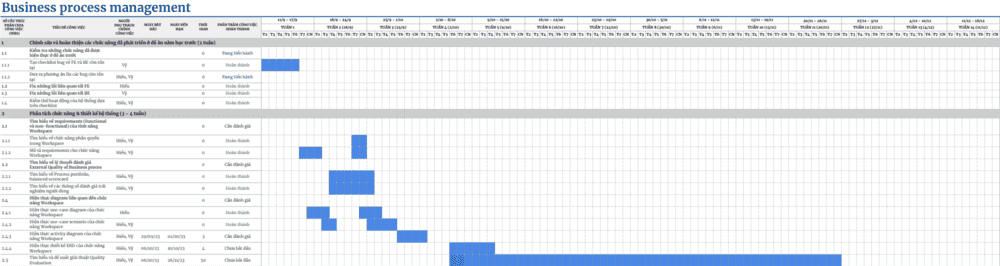
\includegraphics[width = \linewidth]{Content/Giới thiệu đề tài/images/PCCV_HK231_1.png}
    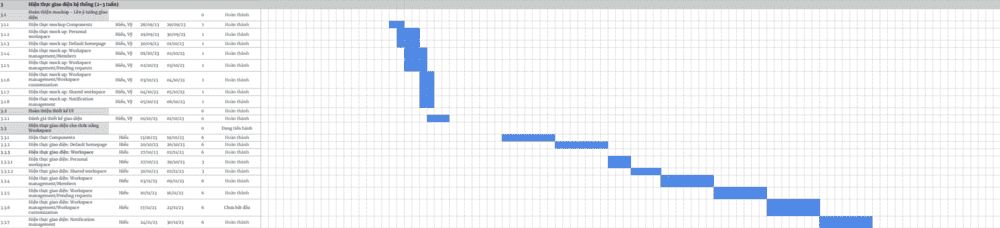
\includegraphics[width = \linewidth]{Content/Giới thiệu đề tài/images/PCCV_HK231_2.png}
    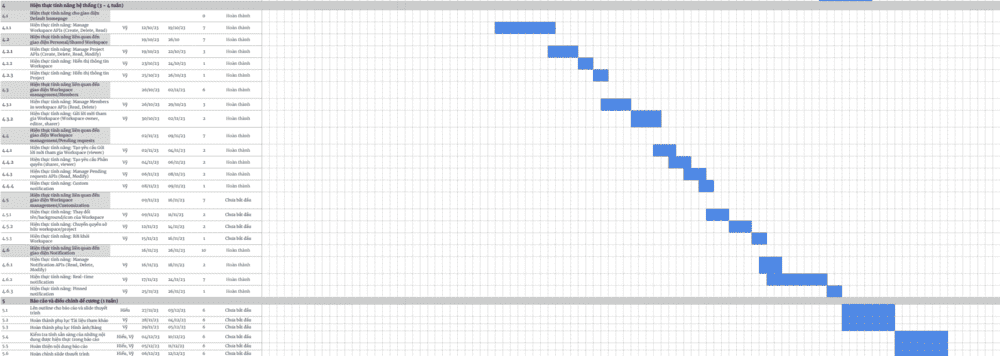
\includegraphics[width = \linewidth]{Content/Giới thiệu đề tài/images/PCCV_HK231_3.png}
    \vspace{0.5cm}
    \caption{Biểu đồ Gantt kế hoạch làm việc giai đoạn học kỳ HK231}
    \label{fig:Biểu đồ Gantt kế hoạch làm việc giai đoạn học kỳ HK231}
\end{figure}

\begin{table}[H]
    \centering
    \def\arraystretch{2}
    \resizebox{\textwidth}{!}{%
    \begin{tabular}{|p{11cm}|p{1.75cm}|p{1.5cm}|p{1.5cm}|}
    \hline
    Mô tả công việc & Phân công & Ngày bắt đầu & Ngày kết thúc 
    \\ \hline
    Hiện thực mockup Components                                             & Hiếu, Vỹ & 28/09/23 & 29/09/23 \\ \hline
    Hiện thực mock up: Personal workspace                                   & Hiếu, Vỹ & 29/09/23 & 30/09/23 \\ \hline
    Hiện thực mock up: Default homepage                                     & Hiếu, Vỹ & 30/09/23 & 01/10/23 \\ \hline
    Hiện thực mock up: Workspace management/Members                         & Hiếu, Vỹ & 01/10/23 & 02/10/23 \\ \hline
    Hiện thực mock up: Workspace management/Pending requests                & Hiếu, Vỹ & 02/10/23 & 03/10/23 \\ \hline
    Hiện thực mock up: Workspace management/Workspace customization         & Hiếu, Vỹ & 03/10/23 & 04/10/23 \\ \hline
    Hiện thực mock up: Shared workspace                                     & Hiếu, Vỹ & 04/10/23 & 05/10/23 \\ \hline
    Hiện thực mock up: Notification management                              & Hiếu, Vỹ & 05/10/23 & 06/10/23 \\ \hline
    Đánh giá thiết kế giao diện                                             & Hiếu, Vỹ & 01/10/23 & 01/10/23 \\ \hline
    Hiện thực Components                                                    & Hiếu     & 13/10/23 & 19/10/23 \\ \hline
    Hiện thực giao diện: Default homepage                                   & Hiếu     & 20/10/23 & 26/10/23 \\ \hline
    Hiện thực giao diện: Personal workspace                                 & Hiếu     & 27/10/23 & 29/10/23 \\ \hline
    Hiện thực giao diện: Shared workspace                                   & Hiếu     & 30/10/23 & 02/11/23 \\ \hline
    Hiện thực giao diện: Workspace management/Members                       & Hiếu     & 03/11/23 & 09/11/23 \\ \hline
    Hiện thực giao diện: Workspace management/Pending requests              & Hiếu     & 10/11/23 & 16/11/23 \\ \hline
    Hiện thực giao diện: Workspace management/Workspace customization       & Hiếu     & 17/11/23 & 23/11/23 \\ \hline
    Hiện thực giao diện: Notification management                            & Hiếu     & 24/11/23 & 30/11/23 \\ \hline
    Hiện thực tính năng: Manage Workspace APIs (Create, Delete, Read)       & Vỹ       & 12/10/23 & 19/10/23 \\ \hline
    Hiện thực tính năng: Manage Project APIs (Create, Delete, Read, Modify) & Vỹ       & 19/10/23 & 22/10/23 \\ \hline
    Hiện thực tính năng: Hiển thị thông tin Workspace                       & Vỹ       & 23/10/23 & 24/10/23 \\ \hline
    Hiện thực tính năng: Hiển thị thông tin Project                         & Vỹ       & 25/10/23 & 26/10/23 \\ \hline
    Hiện thực tính năng: Manage Members in workspace APIs (Read, Delete)    & Vỹ       & 26/10/23 & 29/10/23 \\ \hline
    Hiện thực tính năng: Gửi lời mời tham gia Workspace (Workspace owner, editor, sharer) & Vỹ       & 30/10/23 & 02/11/23 \\ \hline
    Hiện thực tính năng: Tạo yêu cầu Gửi lời mời tham gia Workspace (viewer)              & Vỹ       & 02/11/23 & 04/11/23 \\ \hline
    Hiện thực tính năng: Tạo yêu cầu Phân quyền (sharer, viewer)            & Vỹ       & 04/11/23 & 06/11/23 \\ \hline
    \end{tabular}%
    }
    \caption{Bảng kế hoạch công việc học kỳ HK231 - phần 1}
\end{table}

\begin{table}[H]
    \centering
    \def\arraystretch{2}
    \resizebox{\textwidth}{!}{%
    \begin{tabular}{|p{11cm}|p{1.75cm}|p{1.5cm}|p{1.5cm}|}
    \hline
    Hiện thực tính năng: Manage Pending requests APIs (Read, Modify)        & Vỹ       & 06/11/23 & 08/11/23 \\ \hline
    Hiện thực tính năng: Custom notification                                & Vỹ       & 08/11/23 & 09/11/23 \\ \hline
    Hiện thực tính năng: Thay đổi tên/background/icon của Workspace         & Vỹ       & 09/11/23 & 11/11/23 \\ \hline
    Hiện thực tính năng: Chuyển quyền sở hữu workspace/project              & Vỹ       & 12/11/23 & 14/11/23 \\ \hline
    Hiện thực tính năng: Rời khỏi Workspace                                 & Vỹ       & 15/11/23 & 16/11/23 \\ \hline
    Hiện thực tính năng: Manage Notification APIs (Read, Delete, Modify)    & Vỹ       & 16/11/23 & 18/11/23 \\ \hline
    Hiện thực tính năng: Real-time notification                             & Vỹ       & 17/11/23 & 24/11/23 \\ \hline
    Hiện thực tính năng: Pinned notification                                & Vỹ       & 25/11/23 & 26/11/23 \\ \hline
    Lên outline cho báo cáo và slide thuyết trình                           & Hiếu     & 27/11/23 & 03/12/23 \\ \hline
    Hoàn thành phụ lục Tài liệu tham khảo                                   & Vỹ       & 28/11/23 & 04/12/23 \\ \hline
    Hoàn thành phụ lục Hình ảnh/Bảng                                        & Vỹ       & 29/11/23 & 05/12/23 \\ \hline
    Kiểm tra tính sẵn sàng của những nội dung được hiện thực trong báo cáo                & Hiếu, Vỹ & 04/12/23 & 10/12/23 \\ \hline
    Hoàn thiện nội dung báo cáo                                             & Hiếu, Vỹ & 05/12/23 & 11/12/23 \\ \hline
    Hoàn chỉnh slide thuyết trình                                           & Hiếu, Vỹ & 06/12/23 & 12/12/23 \\ \hline
    \end{tabular}%
    }
    \caption{Bảng kế hoạch công việc học kỳ HK231 - phần 2}
\end{table}

\subsection{Giai đoạn học kỳ HK232}

\begin{figure} [H]
    \centering
    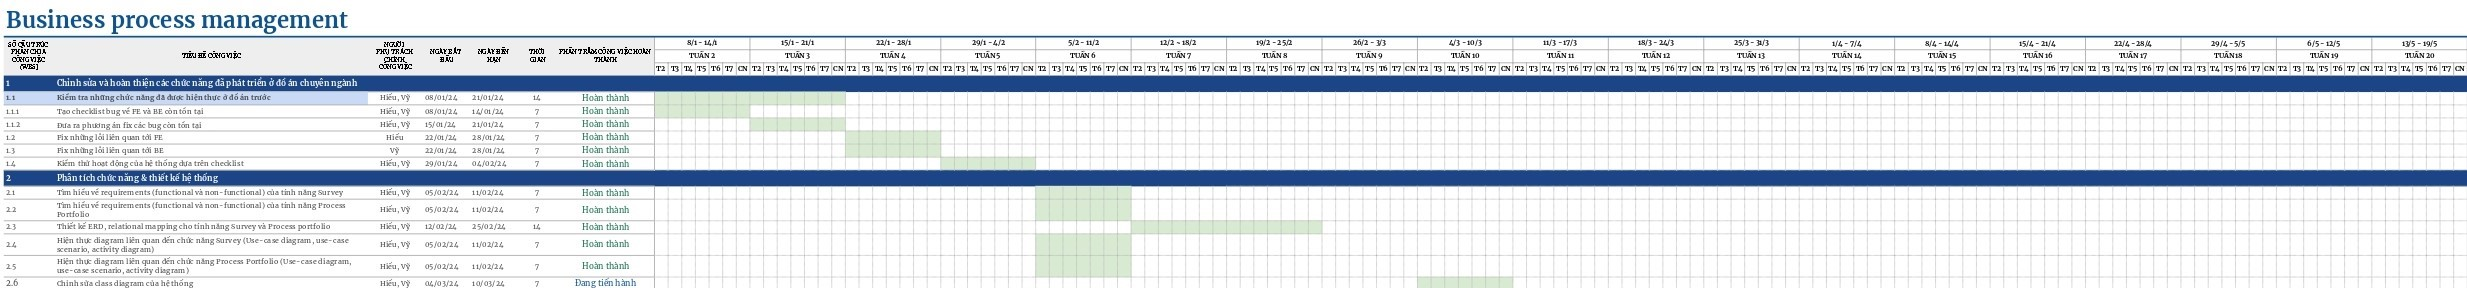
\includegraphics[width = \linewidth]{Content/Giới thiệu đề tài/images/PCCV_HK232_1.jpg}
    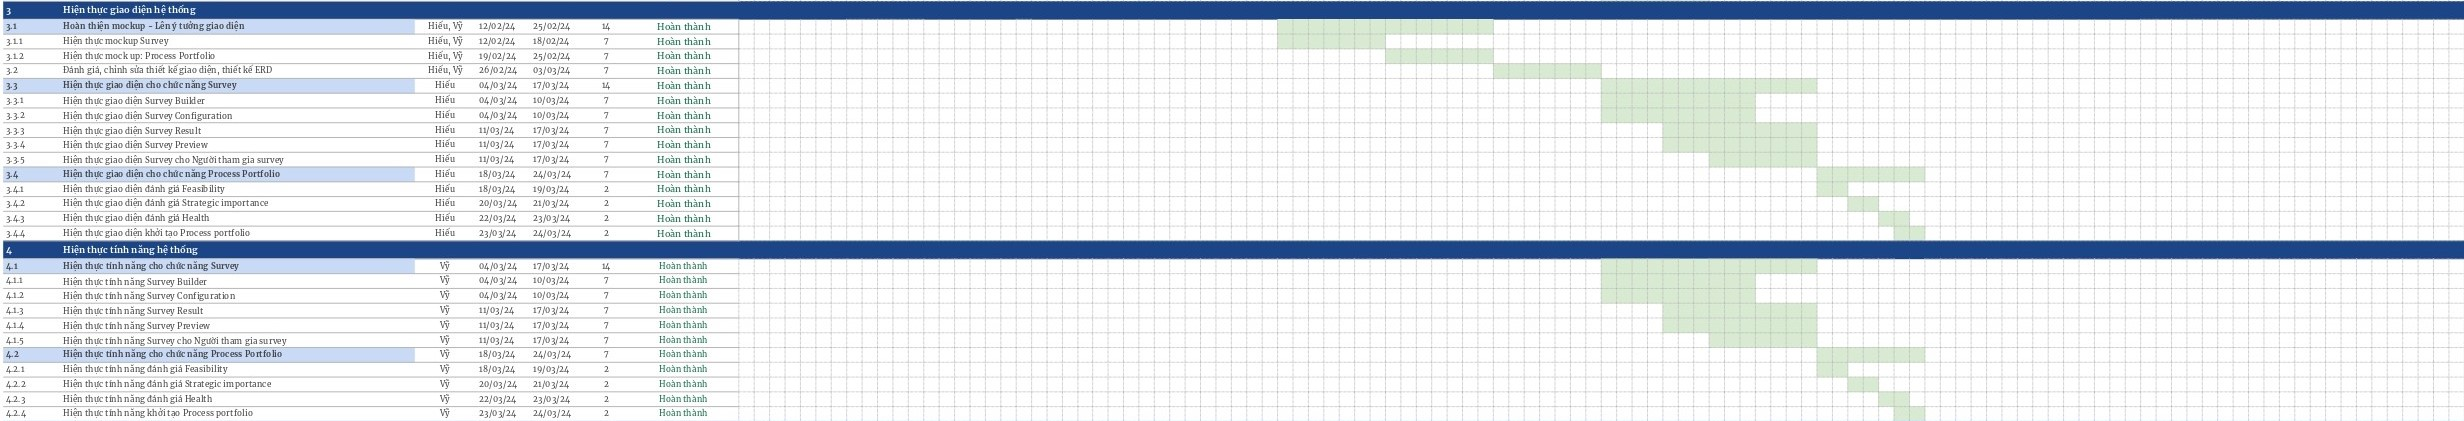
\includegraphics[width = \linewidth]{Content/Giới thiệu đề tài/images/PCCV_HK232_2.jpg}
    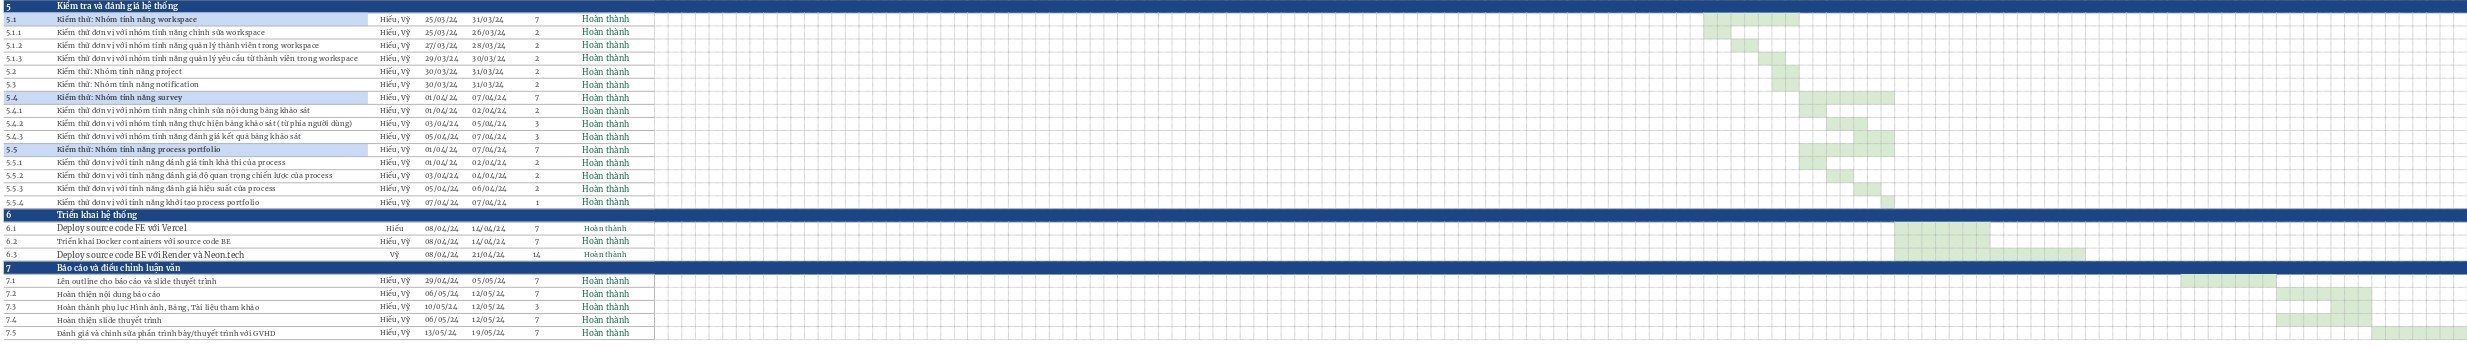
\includegraphics[width = \linewidth]{Content/Giới thiệu đề tài/images/PCCV_HK232_3.jpg}
    \vspace{0.5cm}
    \caption{Biểu đồ Gantt kế hoạch làm việc giai đoạn học kỳ HK232}
    \label{fig:Biểu đồ Gantt kế hoạch làm việc giai đoạn học kỳ HK232}
\end{figure}

\begin{table}[H]
    \centering
    \def\arraystretch{2}
    \resizebox{\textwidth}{!}{%
    \begin{tabular}{|p{11cm}|p{1.75cm}|p{1.5cm}|p{1.5cm}|}
    \hline
    Mô tả công việc & Phân công & Ngày bắt đầu & Ngày kết thúc
        \\ \hline
        { Tìm hiểu về requirements (functional và non-functional) của tính năng Survey} &
        { Hiếu, Vỹ} &
        { 05/02/24} &
        { 11/02/24} \\ \hline
        { Tìm hiểu về requirements (functional và non-functional) của tính năng Process Portfolio} &
        { Hiếu, Vỹ} &
        { 05/02/24} &
        { 11/02/24} \\ \hline
        { Thiết kế ERD, relational mapping cho tính năng Survey và Process portfolio} &
        { Hiếu, Vỹ} &
        { 12/02/24} &
        { 25/02/24} \\ \hline
        { Hiện thực diagram liên quan đến chức năng Survey (Use-case diagram, use-case scenario, activity diagram)} &
        { Hiếu, Vỹ} &
        { 05/02/24} &
        { 11/02/24} \\ \hline
        { Hiện thực diagram liên quan đến chức năng Process Portfolio (Use-case diagram, use-case scenario, activity diagram)} &
        { Hiếu, Vỹ} &
        { 05/02/24} &
        { 11/02/24} \\ \hline
        { Chỉnh sửa class diagram của hệ thống} &
        { Hiếu, Vỹ} &
        { 04/03/24} &
        { 10/03/24} \\ \hline
        { Hiện thực mockup Survey} &
        { Hiếu, Vỹ} &
        { 12/02/24} &
        { 18/02/24} \\ \hline
        { Hiện thực mock up: Process Portfolio} &
        { Hiếu, Vỹ} &
        { 19/02/24} &
        { 25/02/24} \\ \hline
        { Đánh giá, chỉnh sửa thiết kế giao diện, thiết kế ERD} &
        { Hiếu, Vỹ} &
        { 26/02/24} &
        { 03/03/24} \\ \hline
        { Hiện thực giao diện Survey Builder} &
        { Hiếu} &
        { 04/03/24} &
        { 10/03/24} \\ \hline
        { Hiện thực giao diện Survey Configuration} &
        { Hiếu} &
        { 04/03/24} &
        { 10/03/24} \\ \hline
        { Hiện thực giao diện Survey Result} &
        { Hiếu} &
        { 11/03/24} &
        { 17/03/24} \\ \hline
        { Hiện thực giao diện Survey Result (trên toàn bộ câu hỏi)} &
        { Hiếu} &
        { 22/04/24} &
        { 28/04/24} \\ \hline{ Hiện thực giao diện Survey Preview} &
        { Hiếu} &
        { 11/03/24} &
        { 17/03/24} \\ \hline
        { Hiện thực giao diện Survey cho Người tham gia survey} &
        { Hiếu} &
        { 11/03/24} &
        { 17/03/24} \\ \hline
        { Hiện thực giao diện đánh giá Feasibility} &
        { Hiếu} &
        { 18/03/24} &
        { 19/03/24} \\ \hline
        { Hiện thực giao diện đánh giá Strategic importance} &
        { Hiếu} &
        { 20/03/24} &
        { 21/03/24} \\ \hline
        { Hiện thực giao diện đánh giá Health} &
        { Hiếu} &
        { 22/03/24} &
        { 23/03/24} \\ \hline
        { Hiện thực giao diện khởi tạo Process portfolio} &
        { Hiếu} &
        { 23/03/24} &
        { 24/03/24} \\ \hline
        { Hiện thực tính năng Survey Builder} &
        { Vỹ} &
        { 04/03/24} &
        { 10/03/24} \\ \hline        
        { Hiện thực tính năng Survey Configuration} &
        { Vỹ} &
        { 04/03/24} &
        { 10/03/24} \\ \hline
        { Hiện thực tính năng Survey Result} &
        { Vỹ} &
        { 11/03/24} &
        { 17/03/24} \\ \hline
        { Hiện thức tính năng Survey Result (trên toàn bộ câu hỏi)} &
        { Vỹ} &
        { 22/04/24} &
        { 28/04/24} \\ \hline
    \end{tabular}%
    }
    \caption{Bảng kế hoạch công việc học kỳ HK232 - phần 1}
\end{table}

\begin{table}[H]
    \centering
    \def\arraystretch{2}
    \resizebox{\textwidth}{!}{%
    \begin{tabular}{|p{11cm}|p{1.75cm}|p{1.5cm}|p{1.5cm}|}
    \hline
    Mô tả công việc & Phân công & Ngày bắt đầu & Ngày kết thúc
        \\ \hline
        { Hiện thực tính năng Survey Preview} &
        { Vỹ} &
        { 11/03/24} &
        { 17/03/24} \\ \hline
        { Hiện thực tính năng Survey cho Người tham gia survey} &
        { Vỹ} &
        { 11/03/24} &
        { 17/03/24} \\ \hline
        { Hiện thực tính năng đánh giá Feasibility} &
        { Vỹ} &
        { 18/03/24} &
        { 19/03/24} \\ \hline
        { Hiện thực tính năng đánh giá Strategic importance} &
        { Vỹ} &
        { 20/03/24} &
        { 21/03/24} \\ \hline
        { Hiện thực tính năng đánh giá Health} &
        { Vỹ} &
        { 22/03/24} &
        { 23/03/24} \\ \hline
        { Hiện thực tính năng khởi tạo Process portfolio} &
        { Vỹ} &
        { 23/03/24} &
        { 24/03/24} \\ \hline
        { Kiểm thử đơn vị với nhóm tính năng chỉnh sửa workspace} &
        { Hiếu, Vỹ} &
        { 25/03/24} &
        { 26/03/24} \\ \hline
        { Kiểm thử đơn vị với nhóm tính năng quản lý thành viên trong workspace} &
        { Hiếu, Vỹ} &
        { 27/03/24} &
        { 28/03/24} \\ \hline
        { Kiểm thử đơn vị với nhóm tính năng quản lý yêu cầu từ thành viên trong workspace} &
        { Hiếu, Vỹ} &
        { 29/03/24} &
        { 30/03/24} \\ \hline
        { Kiểm thử: Nhóm tính năng project} &
        { Hiếu, Vỹ} &
        { 30/03/24} &
        { 31/03/24} \\ \hline
        { Kiểm thử: Nhóm tính năng notification} &
        { Hiếu, Vỹ} &
        { 30/03/24} &
        { 31/03/24} \\ \hline
        { Kiểm thử đơn vị với nhóm tính năng chỉnh sửa nội dung bảng khảo sát} &
        { Hiếu, Vỹ} &
        { 01/04/24} &
        { 02/04/24} \\ \hline
        { Kiểm thử đơn vị với nhóm tính năng thực hiện bảng khảo sát (từ phía người dùng)} &
        { Hiếu, Vỹ} &
        { 03/04/24} &
        { 05/04/24} \\ \hline
        { Kiểm thử đơn vị với nhóm tính năng đánh giá kết quả bảng khảo sát} &
        { Hiếu, Vỹ} &
        { 05/04/24} &
        { 07/04/24} \\ \hline
        { Kiểm thử đơn vị với tính năng đánh giá tính khả thi của process} &
        { Hiếu, Vỹ} &
        { 01/04/24} &
        { 02/04/24} \\ \hline
        { Kiểm thử đơn vị với tính năng đánh giá độ quan trọng chiến lược của process} &
        { Hiếu, Vỹ} &
        { 03/04/24} &
        { 04/04/24} \\ \hline
        { Kiểm thử đơn vị với tính năng đánh giá hiệu suất của process} &
        { Hiếu, Vỹ} &
        { 05/04/24} &
        { 06/04/24} \\ \hline
        { Kiểm thử đơn vị với tính năng khởi tạo process portfolio} &
        { Hiếu, Vỹ} &
        { 07/04/24} &
        { 07/04/24} \\ \hline
        { Deploy source code FE với Vercel} &
        { Hiếu} &
        { 08/04/24} &
        { 14/04/24} \\ \hline
        { Triển khai Docker containers với source code BE} &
        { Hiếu, Vỹ} &
        { 08/04/24} &
        { 14/04/24} \\ \hline
        { Deploy source code BE với Render và Neon.tech} &
        { Vỹ} &
        { 08/04/24} &
        { 21/04/24} \\ \hline
        { Lên outline cho báo cáo và slide thuyết trình} &
        { Hiếu, Vỹ} &
        { 29/04/24} &
        { 05/05/24} \\ \hline
        { Hoàn thiện nội dung báo cáo} &
        { Hiếu, Vỹ} &
        { 06/05/24} &
        { 12/05/24} \\ \hline
        { Hoàn thành phụ lục Hình ảnh, Bảng, Tài liệu tham khảo} &
        { Hiếu, Vỹ} &
        { 10/05/24} &
        { 12/05/24} \\ \hline
        { Hoàn thiện slide thuyết trình} &
        { Hiếu, Vỹ} &
        { 06/05/24} &
        { 12/05/24} \\ \hline
        { Đánh giá và chỉnh sửa phần trình bày/thuyết trình với GVHD} &
        { Hiếu, Vỹ} &
        { 13/05/24} &
        { 19/05/24} \\ \hline
    \end{tabular}%
    }
    \caption{Bảng kế hoạch công việc học kỳ HK232 - phần 2}
\end{table}
\newpage
\chapter{Cơ sở lý thuyết}
\section{Business Project Evaluation}

\subsection{Thời gian chu kỳ}
Thời gian chu kỳ của một quy trình được tính toán dựa trên thời gian chu kỳ của từng hoạt động trong quy trình đó. Thời gian được sử dụng ở đây là thời gian lý thuyết, không tính thời gian thực tế.
Quy trình nghiệp vụ được chia thành các khối nhỏ hơn. Khi tính toán được thời gian chu kỳ của từng khối, có thể dễ dàng tính toán được chu kỳ của cả quy trình.
\begin{itemize}
    \item Khối tuần tự (sequential fragment): thời gian chu kỳ của 1 khối tuần tự bằng với thời gian chu kỳ của các hoạt động trong khối đó:
 \[ CT =\sum_{i=1}^{n} T_i \]
   \item Khối XOR (Exclusive gateway): khối được bắt đầu và kết thúc bởi 2 cổng XOR, trong trường hợp này cần quan tâm tới xác suất rẽ nhánh của từng nhánh đi ra từ cổng XOR, ta ký hiệu là p:
   \[ CT =\sum_{i=1}^{n} p_i \times T_i \]
   \item Khối AND (parallel gateway): Khối được bắt đầu và kết thúc bởi 2 cổng AND, ta cần biết thời gian lớn nhất mà các nhánh cần để thực thi khối AND này.
   \[ CT = Max(T_1, T_2,..., T_n) \]
   \item Vòng lặp (rework pattern): Một chuỗi các hoạt động hoặc một hoạt động được lặp đi lặp lại với tần suất $r$ nào đó, ta có công thức tính thời gian chu kỳ của vòng lặp:
   \[ CT = \frac{T}{1 - r}\]
   Với T là tổng thời gian chu kỳ của khối lặp này
   \item Khối OR (inclusive gateway): Khối được bắt đầu và kết thúc bởi 2 cổng OR, cho phép ta chọn được một hoặc nhiều hơn một nhánh được rẽ ra từ cổng này. Công thức tổng quát cho khối OR:
   \[ CT = Max(T_1, T_2,..., T_i)\]
   Với $T_1$, $T_2$,..., $T_i$ là những nhánh được xác định sẽ được chạy trong khối OR này và $i <= n$ với $n$ là tất cả các nhánh trong khối OR. Các nhánh được chạy sẽ được xác định ngay từ đầu.
\end{itemize}
\subsection{Chi phí}
Trong đề tài này, tương tự như đề tài trước, chúng tôi vẫn dựa trên mô hình chi phí dựa trên hoạt động theo thời gian \emph{Time-driven activity-based costing
model} - chi phí được tính dựa trên thời gian cần thiết để thực hiện một tác vụ có trong quy trình và chi phí đơn vị (unit cost) của khả năng cung ứng (supplying capacity) theo thời gian. Công thức tính như sau:
\[ C = UC \times T \tag*{\cite{prereport}}\]
\par
Trong đó C là tổng chi phí của cả quy trình, T là thời gian chu kỳ của quy trình và UC (unit cost) là chi phí đơn vị của quy trình đó. Chi phí đơn vị được tính như sau:
\[ UC = \frac{CTT}{PC} \tag*{\cite{prereport}}\]
\par
Trong đó \emph{CTT} là tổng số thời gian mà một đơn vị (phòng ban) trong tổ chức có thể bỏ ra trong một đơn vị thời gian. \emph{PC} là chi phí có thể cung cấp cho một đơn vị của tổ chức trong một đơn vị thời gian.
\subsection{Độ minh bạch}
Tính minh bạch của một quy trình trong một khung nhìn (lane) cụ thể được xác định bởi số lượng tác vụ minh bạch trong khung nhìn tương ứng so với tổng số tác vụ minh bạch hiện có trong quy trình đó trong khung nhìn tổng quát. Một hoạt động được xem như là minh bạch khi nó không phải là một Quy trình phụ - \emph{sub - process} hay một hoạt động tham chiếu đến một quy trình bên ngoài, còn gọi là Hoạt động gọi - \emph{call - activity}:
\[ \text{Transparent Level (specific view)}  = \frac{\text{Num of explicit tasks (specific view)} }{\text{Num of explicit tasks (full view)}} \tag*{\cite{prereport}}\]

\subsection{Khả năng xử lý ngoại lệ}
Ngoại lệ là những sự kiện khiến cho quy trình đi từ luồng thông thường sang tình huống không mong đợi và không thường xảy ra. Có thể đó là những lỗi trong quy trình nghiệp vụ hoặc lỗi về mặt kỹ thuật. Công thức tính độ xử lý ngoại lệ như sau:
\[ \text{Exception handling level } = \frac{\text{Num of handled exceptions}}{\text{Num of handled exceptions + Num of unhandled exceptions}} \tag*{\cite{prereport}}\]
\par
Chúng tôi cùng với đề tài trước quy định để biểu
diễn một ngoại lệ, người dùng phải biểu diễn bằng các sự kiện lỗi \emph{(error event)}, nếu như sự kiện đó dẫn ra một hoạt động khác thì ngoại lệ đó được xem như là đã được xử lý. Còn lại các ngoại lệ khác sẽ được xem như chưa được xử lý.
\subsection{Độ linh hoạt}
Độ linh hoạt được biểu diễn bằng số lượng biến thể có thể có của một quy trình. Biến thể được tạo ra vì chúng có các khối hay các nhánh không phải thực thi. Độ linh hoạt của một quy trình được tính như sau:
\[F = \frac{\text{Num of optional tasks}}{\text{Num of total tasks}} \tag*{\cite{prereport}}\]
\par
Với \emph{Num of optional tasks} là số lượng tasks có trong khối XOR, và \emph{Num of total tasks} là tổng các tasks có trong quy trình đó.
\subsubsection{Chất lượng}
Chất lượng là một khái niệm trừu tượng và khó để mô hình hoá cụ thể. Ở đề tài trước, chất lượng của quy trình được đo lường dựa trên xác suất lặp lại $r$ của các khối lặp, với công thức tính như sau:
\[ Q = 1 - \frac{(r_1 + r_2 + ... + r_n)}{n}\]
trong đó $r_1$, $r_2$,..., $r_n$ là xác suất lặp lại của các vòng lặp trong quy trình, $n$ là tổng số vòng lặp có trong quy trình.
\par
Tuy nhiên, ở đề tài này, chúng tôi nhận thấy chất lượng của một quy trình không chỉ đến từ xác suất của các vòng lặp trong quy trình, mà nó còn có thể bị tác động bởi nhiều yếu tố khác. Chất lượng của một quy trình có thể được xem xét ở hai góc nhìn khác nhau: góc nhìn từ phía người sở hữu quy trình hay người thiết kế quy trình, và góc nhìn của người tham gia sử dụng, vận hành quy trình, sử dụng sản phẩm, dịch vụ của quy trình đó trên thực tế. Đây cũng có thể được xem lần lượt là \emph{internal quality} (chất lượng bên trong) và \emph{external quality} (chất lượng bên ngoài). 
\par
\emph{Internal quality} của một quy trình nghiệp vụ được xem như chất lượng quy trình trong quá trình thiết kế. Ở đây, chúng tôi cho rằng \emph{internal quality} có thể được xem như chất lượng gắn liền với số lượng và xác suất của các vòng lặp có trong quy trình, được biểu diễn và tính toán như trên. Mặt khác, \emph{external quality} lạ được đánh giá bởi sự hài lòng và trải nghiệm của những người sử dụng, tham gia vận hành hay sử dụng sản phẩm, dịch vụ của quy trình nghiệp vụ đó trong thực tế. Sự hài lòng đối với một quy trình có thể được diễn tả như mức độ mà người dùng (khách hàng) cảm nhận liệu quy trình nghiệp vụ có đáp ứng được nhu cầu của họ hay không. Sự hài lòng này không chi đơn thuần là cảm nhận trừu tượng, mà nó có thể được đo đạc với những giá trị cụ thể biểu thị cho mức độ của nó. Việc đo lường này giúp phản ánh được thái độ và kỳ vọng của khách hàng một cách hiệu quả, trực tiếp, có ý nghĩa, có thể tham khảo và so sánh. 
% Bằng cách này, sự hài lòng của khách hàng sẽ là một tiêu chuẩn cơ bản cho hiệu suất của bất kỳ sản phẩm hay dịch vụ nào, cụ thể ở đây là một quy trình nghiệp vụ trên thực tế.
\section{Process portfolio}

Nhìn vào thực tế, quy trình nghiệp vụ thường gắn liền với một tổ chức hoặc công ty, vì vậy việc quản lý quy trình nghiệp vụ liên quan đến một nhóm những quy trình có ảnh hưởng tới nhau. 

Tuy nhiên, không phải tất cả những bên liên quan (stakeholders) phụ trách quản lý quy trình nghiệp vụ đều có được cái nhìn tổng quát về toàn bộ quy trình trong tổ chức của họ. 

Việc đặt ra nhu cầu nắm bắt được bức tranh tổng quát về hệ thống quy trình trong tổ chức là cần thiết, từ đó chúng ta có thể đưa ra những quyết định liên quan tới việc giám sát hiệu suất của quy trình hoặc thay đổi, chỉnh sửa quy trình đó.

Với mong muốn hỗ trợ những người quản lý quy trình nghiệp vụ có được góc nhìn chính xác về việc xác định những quy trình nào thì cần được cải tiến, hệ thống BPSky hình thành nên Danh mục quy trình (trong ngữ cảnh của hệ thống thì chúng ta sẽ thống nhất dùng từ Process portfolio). 

\begin{figure}[H]
    \begin{center}
        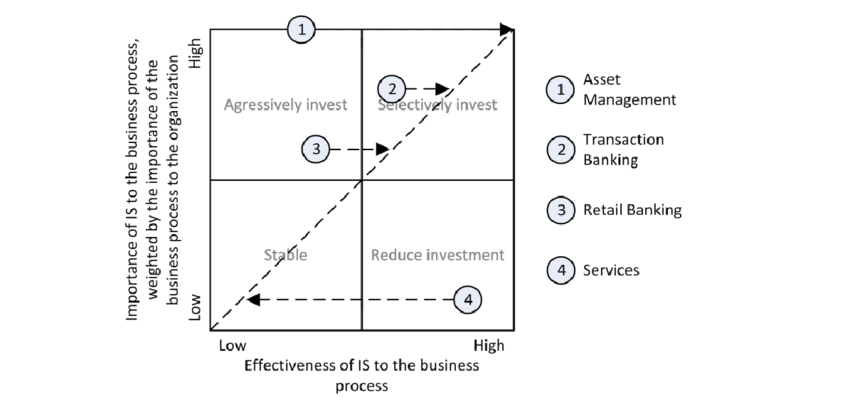
\includegraphics[width=0.8\textwidth]{Content/Cơ sở lý thuyết/documents/Process portfolio/images/ProcessPortfolioIllustration.png}
        \vspace{0.5cm}
        \caption{Ví dụ về Danh mục quy trình (Process portfolio)}
        \label{fig: Ví dụ về Danh mục quy trình (Process portfolio)}
    \end{center}
\end{figure}

Process portfolio đề cập tới một lược đồ có nhiệm vụ trực quan hóa những quy trình nghiệp vụ thông qua những tiêu chí được đề ra. Những quy trình được biểu diễn dưới dạng những node, thông tin của từng node sẽ được cung cấp từ phía người dùng và cả từ những đánh giá của hệ thống về mô hình quy trình nghiệp vụ hiện tại.

Process portfolio giúp người quản lý hình dung được mức độ ưu tiên giữa những quy trình nghiệp vụ, đây là cơ sở để chúng ta có được những bước đi kế tiếp liên quan tới việc phân tích, đánh giá, tái thiết kế quy trình.
% \subsection{Process selection}
Quá trình phân loại mức độ ưu tiên của quy trình nghiệp vụ sẽ dựa trên 3 tiêu chí: Độ quan trọng chiến lược (Strategic importance), Sức khỏe (Health), Tính khả thi (Feasibility).

\subsubsection{Độ quan trọng chiến lược}
    Mức độ quan trọng chiến lược liên quan tới sự ảnh hưởng hoặc giá trị của một quy trình đối với việc đạt được mục tiêu lâu dài của tổ chức. Những quy trình này có thể liên quan tới tính độc quyền thương hiệu, quy trình đóng góp vào việc tạo ra lợi thế cạnh tranh trong thị trường đối với các đối thủ khác hoặc quy trình đóng góp vào việc tạo ra giá trị cho khách hàng và đem lại nguồn lợi nhuận chính.

Việc xác định được tầm quan trọng của quy trình đối với chiến lược của tổ chức sẽ là chìa khóa giúp chúng ta nhìn ra được những quy trình trọng tâm cần nhắm tới khi muốn phát triển bền vững và lâu dài.
\subsubsection{Sức khỏe}
    Health, hay gọi là Công năng của quy trình, là tiêu chí nhắm vào việc đánh giá mức độ hiệu quả và hiệu suất hoạt động của quy trình nghiệp vụ. Nó đo lường khả năng tổ chức thực hiện quy trình một cách hiệu quả, tiết kiệm và linh hoạt xử lý các trường hợp ngoại lệ nhưng cũng đồng thời đảm bảo các tiêu chuẩn về đầu ra.

Việc đánh giá tiêu chí này sẽ dễ dàng với những tổ chức hoạt động hướng quy trình - xác định nghiệp vụ dưới dạng những quy trình nghiệp vụ có thể mô hình hóa được; đây là một lợi thế cho phép doanh nghiệp thu thập được những thông tin cần thiết cho quá trình đánh giá hiệu suất. Cụ thể hơn, việc đánh giá hiệu suất quy trình nghiệp vụ sẽ được mô tả thông qua 4 tiêu chí: thời gian (time), chi phí (cost), chất lượng (quality) và độ linh hoạt (flexibility).

\subsubsection{Thời gian}

Thời gian là yếu tổ phổ biến trong đánh giá hiệu suất quy trình nghiệp vụ. Cụ
thể hơn thì đại lượng được tính toán phổ biến là thời gian chu kỳ (cycle time)
- khoảng thời gian mà quy trình nghiệp vụ bắt đầu cho đến khi kết thúc; đây là
đại lượng được tập trung tính toán ở hệ thống tiền nhiệm (BKSky 1.0) nhằm mục
đích đánh giá quy trình nghiệp vụ.

Mục tiêu của đa phần những quy trình nghiệp vụ là giảm thời gian chu kỳ thực
tế, điều này có thể hiểu là giảm thời gian chờ đợi (waiting time) - khoảng thời
gian mà quy trình chờ để nhận được phản hồi từ người dùng; hoặc thời gian phục
vụ (serving time) - khoảng thời gian thực sự tiêu tốn để hoàn thành tác vụ quy
định trong quy trình nghiệp vụ.

Trong ngữ cảnh của hệ thống hiện tại, chúng ta vẫn sẽ tập trung vào đánh giá
hiệu suất của quy trình dựa vào đại lượng thời gian chu kỳ (cycle time).

\subsubsection{Chi phí}

Khía cạnh về chi phí là khía cạnh phổ biến được cân nhắc trong giai đoạn phân
tích, đánh giá và tái thiết kế quy trình. Khi chúng ta đề cập tới chi phí, mục
tiêu đi kèm là giảm thiểu chi phí được sử dụng để vận hành quy trình nghiệp vụ.
Chi phí này có thể là chi phí cố định (fixed cost) - chi phí không bị ảnh hưởng
bởi cường độ và tần suất vận hành của quy trình nghiệp, thường là chi phí sử
dụng cơ sở vật chất, chi phí bảo trì hệ thống,...; hoặc chi phí biến đổi
(variable cost) - chi phí liên quan tới "lượng", ví dụ phụ thuộc vào số lượng
sản phẩm, số lượng nhân viên,...

Kế thừa ngữ cảnh của hệ thống cũ, hệ thống BKSky 2.0 sẽ xem xét khía cạnh chi
phí theo mô hình Chi phí dựa trên hoạt động theo thời gian (Time-driven
activity-based costing model); trong mô hình này chúng ta sẽ quan tâm tới chi
phí đơn vị (unit cost) mà tổ chức chi trả cho quy trình nghiệp vụ để thực thi,
vận hành trong một đơn vị thời gian.

\subsubsection{Chất lượng}

Như đã trình bày ở trên, chất lượng của quy trình có thể được nhìn nhận dưới hai góc nhìn chính: bên
trong (internal quality) và bên ngoài (external quality). Chất lượng quy trình
là khái niệm có phần trừu tượng, định nghĩa chất lượng có thể được tổng hợp từ
nhiều yếu tố nhỏ liên quan; tuy nhiên trong ngữ cảnh hệ thống hiện tại, chúng
ta sẽ tập trung phản ánh chất lượng của quy trình thông qua tính dễ hiểu của
quy trình đối với người tham gia quy trình (process's participants - phân biệt
với khách hàng sử dụng sản phẩm/dịch vụ cung cấp bởi đầu ra của quy trình).

Kế thừa ngữ cảnh của hệ thống BKSky 1.0, thời gian của các tác vụ trong khối
lặp trong quy trình ảnh hưởng theo một trọng số lớn đến tổng thời gian của cả
quy trình. Vì vậy xác suất lặp của khối lặp càng lớn thì khả năng nó tác động
đến tổng thời gian của quy trình càng cao, chất lượng bên trong của quy trình
sẽ bị ảnh hưởng bởi xác suất lặp của các khối lặp. Yếu tố này sẽ được kế thừa
trong hệ thống hiện tại.

Bên cạnh đó, phản hồi từ phía người tham gia quy trình nghiệp vụ cũng đóng góp
vào việc đánh giá chất lượng của quy trình. Phản hồi có thể được thu thập thông
qua khảo sát hoặc những lời góp ý từ phía người tham gia quy trình. Hệ thống
hiện tại sẽ tập trung vào việc khai thác phản hồi từ phía người dùng để hoàn
thiện hơn quá trình đánh giá chất lượng của quy trình nghiệp vụ.

\subsubsection{Độ linh hoạt}

Độ linh hoạt của quy trình thể hiện thông qua khả năng thay đổi để thích nghi dưới những điều kiện khác nhau của quy trình nghiệp vụ. Tổ chức thường có mong muốn khiến quy trình nghiệp vụ của họ nhanh hơn, rẻ hơn và tốt hơn mà không chú ý đến yếu tố thay đổi của quy trình. Có thể dưới những hoàn cảnh khác nhau, tính ổn định vốn có của quy trình sẽ đánh mất hoàn toàn; khi đó, để so sánh hai quy trình với nhau thì quy trình có thể hoạt động ổn định trong đa số hoàn cảnh lại chiếm ưu thế hơn quy trình hoạt động tốt khi tải bình thường nhưng lại đình trệ khi tải vượt quá cao.

Mục tiêu là chúng ta cần nâng cao được tính linh hoạt của quy trình để có thể
đáp ứng nhiều điều kiện khác nhau, tính thích ứng có thể thể hiện thông qua:

\begin{itemize}
    \item Run-time flexibility - Khả năng sinh ra luồng thực thi ứng với những điều kiện
          đầu vào khác nhau: Luồng thực thi khi này sẽ được xem xét như là một biến thể
          (variation) của quy trình nghiệp vụ.

    \item Build-time flexibility - Khả năng thay đổi cấu trúc của quy trình ứng với những
          hoàn cảnh khác nhau: Quy trình khi này sẽ sinh ra những phiên bản (version), có
          thể khác biệt về cấu trúc quy trình, nhằm đảm bảo được đầu ra ổn định dưới
          những điều kiện khác nhau.
\end{itemize}

Trong ngữ cảnh của hệ thống BKSky 1.0, chúng ta đã xem xét tính linh hoạt của
quy trình nghiệp vụ bị ảnh hưởng bởi số lượng biến thể sinh ra khi luồng thực
thi rẽ nhánh. Ở hệ thống hiện tại, chúng ta sẽ kế thừa định nghĩa về tính linh hoạt của quy trình vào trong quá trình tính toán và khởi tạo process portoflio.

\subsubsection{Mức độ hiệu suất}

Những tiêu chí được trình bày bên trên đều được đánh giá dưới dạng các đại lượng định tính/định lượng, mỗi đại lượng sẽ được thể hiện thông qua những đơn vị và thang đo khác nhau.

Để có được đánh giá tổng hợp về công năng của quy trình, chúng ta cần đưa những đại lượng này về cùng một thang đo, thông qua việc chuyển đổi đại lượng về cùng một đơn vị đo lường. Để làm được điều này, chúng ta cần xác định một mức độ hiệu suất (performance level) của quy trình nghiệp vụ, mức độ hiệu suất này sẽ phản ánh mức độ đạt được mục tiêu của quy trình nghiệp vụ. Giá trị sẽ này được quy về khoảng giá trị từ (-1, 1).

Trước tiên, chúng ta biết rằng một đại lượng có thể là tích cực (positive), tiêu cực (negative) hoặc lưỡng cực (bidirectional); nghĩa rằng chúng ta cần tối đa hóa, tối thiểu hóa hoặc cân bằng giá trị của đại lượng đó để mức độ đạt được mục tiêu của đại lượng tăng. Để làm rõ mục tiêu của đại lượng thì chúng ta cần hiểu được lý do vì sao đại lượng đó là cần thiết. Ví dụ, chỉ số "Thời gian chu kỳ của quy trình" là cần thiết để đánh giá mục tiêu "Tối thiểu hóa thời gian chu kỳ của quy trình".

Sau khi xác định được tính chất của đại lượng, chúng ta quan tâm đến bộ 3 giá trị lần lượt là Target value - Giá trị mục tiêu, Threshold value - Giá trị ngưỡng và Worst value - Giá trị xấu nhất; trong đó:

\begin{align}
      Target{\ }value \geq Threshold{\ }value \geq Worst{\ }value
\end{align}

Ba giá trị này sẽ giúp chúng ta xác định được mức độ hiện tại của chỉ số so với mục tiêu đồng thời giúp đưa những đại lượng có đơn vị khác nhau về một miền giá trị (-1, 1). Current value - Giá trị hiện tại cần được đánh giá, sẽ thông qua công thức biến đổi sau để đưa về giá trị biểu diễn mức độ hiệu suất:

\begin{align}
      pl(current{\ }v.) = \frac{\left| current{\ }v. -{\ }threshold{\ }v.\right|}{\left| target{\ }v. -{\ }threshold{\ }v. \right|} (current {\ }v.\geq  threshold{\ }v.)
\end{align}

hoặc

\begin{align}
      pl(current{\ }v.) = - \frac{\left| current{\ }v. -{\ }threshold{\ }v.\right|}{\left| threshold{\ }v. -{\ }worst{\ }v. \right|} (current {\ }v. <  threshold{\ }v.)
\end{align}
\subsubsection{Tính khả thi}
    Tính khả thi là tiêu chí thứ ba được cân nhắc trong process portfolio; trong phạm vi ngữ cảnh của hệ thống, tính khả thi của quy trình nghiệp vụ sẽ liên quan tới câu hỏi "Quy trình có khả năng mở rộng không?". Thay vì tập trung vào câu hỏi "Quy trình có khả năng hiện thực không?" thì khả năng mở rộng của quy trình trong tương lai sẽ ảnh hưởng nhiều hơn tới quyết định đầu tư tài nguyên và nhân lực của tổ chức. Tính khả thi thể hiện rõ ràng hơn trên con đường phát triển dài về sau; khi mà mục tiêu hiệu suất trở nên ngày càng cao thì doanh nghiệp sẽ phải nỗ lực hơn để liên tục thử nghiệm và thay đổi quy trình nghiệp vụ, quá trình này có thể kèo dài theo năm. Vì vậy để có được điểm khởi đầu tốt thì tính khả thi của quy trình nghiệp vụ là đáng được cân nhắc.
\section{Thiết kế bảng khảo sát}
% Giới thiệu survey %
Đánh giá \emph{external quality} đồng nghĩa với việc đánh giá được sự hài lòng của người dùng hoặc khách hàng đối với một quy trình nghiệp vụ. Để làm được như vậy, cần phải thu thập những ý kiến của người sử dụng hoặc theo dõi và tự động đánh giá quá trình người dùng thực thi quy trình nghiệp vụ. Ngày nay, có một số công cụ dưới dạng các ứng dụng mở rộng (add-on extensions) trên các trình duyệt web, cho phép tích hợp vào hệ thống để theo dõi các luồng thực thi của khách hàng trên một quy trình cụ thể, chẳng hạn như khách hàng có hoàn thành phiên hoạt động của mình hay không, khách hàng có rơi vào những trường hợp ngoại lệ không, có khách hàng nào dừng quy trình giữa chừng hay không.
Ứng dụng các công cụ trên vào đánh giá chất lượng bên ngoài của quy trình có thể đảm bảo tính chính xác, và được thực thi một cách tự động dựa trên việc theo dõi hành vi của người dùng, không tốn nhiều thời gian, công sức của người dùng . Tuy nhiên, không phải quy trình nghiệp vụ nào cũng có thể được tích hợp công cụ trên. Một số quy trình nghiệp vụ cần được thực thi ngoài thực tế, không phải trên các trang web hay hệ thống máy tính, dẫn tới không thể ứng dụng các công cụ theo dõi hành vi người dùng vào những quy trình nghiệp vụ này. Chúng tôi nhận thấy rằng, đối với những loại quy trình này nói riêng, hay cả những quy trình khác nói chung, đều có thể thu thập được sự hài lòng và trải nghiệm của người dùng thông qua các cuộc khảo sát (survey).
\par
Khảo sát đã được ứng dụng từ lâu để lấy ý kiến khách hàng về một dịch vụ, sản phẩm,... hay thậm chí là cả một tổ chức, một doanh nghiệp. Ngày nay, khảo sát vẫn là một công cụ phổ biến và hiệu quả để thu thập thông tin từ người dùng, cho nên ta có thể sử dụng khảo sát, với các câu hỏi khai thác hợp lý, có thể đánh giá được thái độ của khách hàng đối với quy trình nghiệp vụ cụ thể như thế nào, từ đó có thể rút ra được \emph{external quality} của quy trình. Khảo sát có thể được thực thi trên nhiều nền tảng khác nhau với nhiều hình thức khác nhau, chẳng hạn như có thể khảo sát khách hàng thông qua chatbot - là một phần mềm ứng dụng trí tuệ nhân tạo để mô phỏng lại các cuộc trò chuyện với người dùng, thông qua cuộc trò chuyện đó có thể lấy được thông tin từ người dùng. Hoặc có thể là một bảng khảo sát trực tuyến với các câu hỏi đa dạng hình thức được thiết kế sẵn để người dùng trả lời và gửi phản hồi về quy trình đó. Khảo sát trực tuyến có một số lợi ích như sau:
\begin{itemize}
    \item Người dùng có thể thực hiện khảo sát bất cứ khi nào họ muốn.
    \item Người dùng có thể dành nhiều thời gian hơn để trả lời các câu hỏi, nói cách khác, họ không bị ràng buộc thời gian.
    \item Khảo sát trực tuyến cho phép người thiết kế đưa ra nhiều hình thức câu hỏi khác nhau để đánh giá nhiều khía cạnh khác nhau của vấn đề cần được khảo sát (câu hỏi hai đáp án, nhiều đáp án, câu hỏi dạng thang điểm,...).
\end{itemize}
\par
Vì một số ưu điểm nêu trên, chúng tôi quyết định lựa chọn khảo sát trực tuyến như là phương tiện chính để đánh giá sự hài lòng của khách hàng đối với quy trình nghiệp vụ.
% Nguyên tắc thiết kế survey %
\subsubsection{Nguyên tắc thiết kế bảng khảo sát}

\paragraph{Nguyên tắc}\mbox{}

Một số nguyên tắc khi thiết kế bảng khảo sát được tổng hợp bên dưới như sau:
\begin{itemize}
    \item Sử dụng từ ngữ đơn giản, quen thuộc, tránh sử dụng các từ ngữ chuyên môn, tiếng lóng, nhiều tầng lớp nghĩa, mơ hồ.
    \item Sử dụng cấu trúc câu đơn giản.
    \item Đưa ra các đáp án lựa chọn đầy đủ, toàn diện, và riêng biệt với nhau.
    \item Tránh những câu hỏi đôi, những câu hỏi phủ định hay phủ định của phủ định.
    \item Tránh những câu hỏi định hướng người dùng buộc phải chọn 
 một đáp án một cách chủ ý.
    \item Những câu hỏi mở đầu nên là những câu hỏi dễ, từ đó xây dựng được sự kết nối giữa người thiết kế câu hỏi và người trả lời câu hỏi.
    \item Các câu hỏi thuộc cùng một chủ đề nên được nhóm lại với nhau.
    \item Các câu hỏi thuộc cùng một chủ đề nên đi từ chung đến riêng.
\end{itemize}

% \paragraph{Câu hỏi đóng và câu hỏi mở}

% Một trong số những điều mà người thiết kế câu hỏi khảo sát nên quan tâm đó là khi nào thì câu hỏi là câu hỏi mở (cho phép người dùng trả lời theo ý kiến cá nhân của họ) hoặc câu hỏi đóng (yêu cầu người dùng lựa chọn đáp án từ các lựa chọn được cung cấp sẵn). Hầu hết phần lớn các bảng khảo sát đều là những câu hỏi đóng, tuy nhiên ở một số khảo sát nghiên cứu, các câu hỏi mở vẫn có vai trò quan trọng.
% \par
% Các câu hỏi mở và đóng cũng có sự khác nhau về khả năng đo lường tính chính xác của tri thức. Các câu hỏi đóng cần phải phán đoán chính xác nhiều hơn câu hỏi mở. Để giải thích cho ý kiến này, Krosnick và Fabrigar đã khảo sát các bài kiểm tra lên học sinh cho thấy rằng các câu hỏi mở cung cấp khả năng đo lường đáng tin cậy hơn các câu hỏi đóng. Mặt khác, các câu hỏi mở lại có nguy cơ cao hơn câu hỏi đóng trong việc nhận những câu trả lời “không biết” từ những người biết đáp án chính xác nhưng họ không chắc chắn về điều đó, hoặc vì họ không thể ngay tức thì nhớ lại đáp án và không thực sự nỗ lực nhớ ra chúng.
% \par
% Vì vậy, các câu hỏi mở có lẽ chỉ phù hợp với những khảo sát mà các phản hồi “không biết” ít có khả năng xảy ra. Các câu hỏi mở cũng làm phong phú kết quả của các cuộc khảo sát mà khó thực hiện những câu hỏi đóng, hoặc các câu hỏi mở có thể được đặt theo sau những câu hỏi đóng để lấy được nhiều thông tin hơn từ người dùng.

\paragraph{Thang điểm}\mbox{}

Việc chọn lựa thang điểm đánh giá cũng là một yếu tố cần được xem xét khi thiết kế bảng câu hỏi khảo sát. Likert (1932) sử dụng thang điểm 5. Osgood, Suci và Tannenbaum (1957) sử dụng thang điểm 7, hay như Thurstone (1928) lại sử dụng thang điểm 11. Không có một quy chuẩn nào cho việc sử dụng thang điểm nào trong khảo sát, dẫu vậy, chúng tôi cho rằng một số thang điểm cụ thể nên được sử dụng để tối ưu hoá dữ liệu thu được từ người dùng. 
Người dùng khi quan sát thang điểm sẽ thực hiện việc đối chiếu các mức điểm với câu trả lời đưa ra và cố gắng tìm kiếm mức điểm trùng khớp nhất có thể. Vì vậy, có một số điều kiện nhất định cần phải được thỏa mãn. 
\begin{itemize}
    \item Thứ nhất, thang đo cần bao phủ các mức độ nhiều nhất có thể, không có ngoại lệ nào.
    \item Thứ hai, các mức điểm trong thang đo cần có sự khác biệt với nhau, ý nghĩa của chúng không đan xen trùng lặp nhau.
    \item Thứ ba, người dùng và người thiết kế câu hỏi phải hiểu được ý nghĩa của mỗi mức điểm và có cách hiểu giống nhau.
\end{itemize}
\par
Nếu một vài trong những điều kiện trên không được đáp ứng có thể ảnh hưởng đến chất lượng của dữ liệu. Ví dụ, nếu câu trả lời người dùng rơi vào một trường hợp nào đó chưa được liệt kê trong thang điểm, nói cách khác, độ chi tiết của thang đo chưa cao dẫn tới chưa có đáp án thực sự phù hợp với câu trả lời của người dùng lúc đó, dẫn tới họ có thể chọn các đáp án khác nhau ở các thời điểm thực hiện khảo sát khác nhau. Ngoài ra, những đáp án có ý nghĩa tương tự nhau (chẳng hạn như “đôi khi” - “thỉnh thoảng”) sẽ khiến người dùng bối rối khi chọn lựa. Khi đó, giả sử như có nhiều người cùng thực hiện bài khảo sát này, họ có thể chọn những đáp án khác nhau vì họ có cách hiểu khác nhau đối với mỗi đáp án mặc dù câu trả lời của họ đưa ra trong đầu là giống nhau.

% \paragraph{Thứ tự câu hỏi}
% Kết quả của cuộc khảo sát có thể bị ảnh hưởng không chỉ bởi cách diễn đạt câu hỏi, mà còn bởi bối cảnh mà câu hỏi được hỏi. Chính vì thế, trong quá trình thiết kế bộ câu hỏi, ta cũng cần quan tâm đến thứ tự các câu hỏi, nhằm tối ưu hoá độ chính xác của các phản hồi và giảm thiểu các sai sót.
% \par
% Các câu hỏi mở đầu có thể đặc biệt ảnh hưởng đến việc người dùng có sẵn sàng hoàn thành khảo sát hay không, vì nó có thể định hình tư tưởng của người dùng rằng khảo sát này nói về cái gì. Chính vì thế, các câu hỏi mở đầu thường thiết lập một kết nối mạnh mẽ đến chủ đề của cuộc khảo sát. Chúng có thể là một tập các câu hỏi đóng và dễ trả lời. Càng về cuối bảng khảo sát, người dùng dần mất đi sự hứng thú ban đầu, có một xu hướng rằng mức độ mất mát dữ liệu tăng lên, các câu hỏi lại càng ít chi tiết hơn và khả năng phân biệt các đáp án của người dùng lại càng giảm.
% \par 
% Cần phải nhóm lại với nhau những câu hỏi có chung chủ đề. Điều này hỗ trợ người dùng nhiều hơn trong việc xử lý thông tin, chẳng hạn như làm rõ ý nghĩa câu hỏi hoặc tìm kiếm trong trí nhớ dễ dàng hơn. 


% Các yếu tố khảo sát %
\subsubsection{Yếu tố khảo sát}
Một số độ đo độ hài lòng của khách hàng đối với một quy trình nghiệp vụ nói riêng và một dịch vụ, sản phẩm nói chung được áp dụng rộng rãi hiện nay có thể kể đến như: \acrfull*{csat}, \acrfull*{ces}, \acrfull*{nps}.

\paragraph{CES}\mbox{}

CES được \acrfull*{ceb} giới thiệu vào năm 2010. CES là dạng câu hỏi đánh giá sự hài lòng của người dùng bằng việc đo đạc nỗ lực của người dùng trong việc tương tác với sản phẩm hay dịch vụ, yêu cầu người dùng đánh giá nỗ lực của họ trên thang điểm từ 1 - 7, với 1 là giá trị cao nhất cho sự không đồng thuận với câu hỏi được đặt ra. 
% Theo CEB Global, điểm CES trên 2.0 được xem như là một giá trị CES tốt. Ngược lại, nếu điểm CES dưới 2.0, đây sẽ là một dấu hiệu cảnh báo cho người thiết kế cần xem xét lại những nguyên nhân dẫn đến việc người dùng không hài lòng và đưa ra những phương hướng giải quyết phù hợp. 
\par
Một số công thức tính CES đã được đưa ra, tuy nhiên mỗi công thức sẽ phù hợp với một số những thang điểm nhất định. Ở đây, chúng tôi chọn thang điểm từ 1 - 7, công thức tính thường gặp sẽ lấy số lượng người đồng ý chia cho tổng số phản hồi từ người dùng và nhân với 10 hoặc 100. Người dùng được xem như là đồng ý khi số điểm họ đánh giá cho câu hỏi này nằm trong tập giá trị \{5, 6, 7\}. Miền giá trị của điểm CES là [0, 1].
\[ \text{CES (\%)} = \frac{\text{Number of positive results}}{\text{Total of respondents}} \times 100 \]
\par
Trong đó \emph{Number of positive results} là số lượng người dùng đồng ý với câu hỏi, \emph{Total of respondents} là số lượng người dùng tham gia trả lời câu hỏi. Ví dụ, nếu chúng tôi nhận được 100 phản hồi và 70 trong số đó là phản hồi tích cực, thì điểm CES sẽ là 70\%.
% \par
% Một trong những ưu điểm của CES đó là chúng có thể cho thấy những điểm cần được cải thiện để nâng cao trải nghiệm của người dùng. Bên cạnh đó, kết quả của khảo sát CES sẽ giúp dự đoán hành vi trong tương lai. Theo như nghiên cứu của HBR, khoảng 94\% khách hàng phản hồi rằng tốn ít công sức trong việc tương tác với một doanh nghiệp sẽ mua lại sản phẩm. Và khoảng 88\% trong số đó sẽ chi nhiều tiền hơn. Nghiên cứu này cũng chỉ ra rằng CES có thể cho biết người dùng đề xuất sản phẩm tới những người khác như thế nào và họ nói về nó ra sao. Khoảng 81\% khách hàng phải tốn nhiều công sức cho biết sẽ có ý kiến tiêu cực về sản phẩm. Cho nên, ta có thể nói rằng nếu người dùng tốn ít công sức trải nghiệm sản phẩm dịch vụ hơn sẽ cho thấy thái độ tích cực của họ đối với sản phẩm, dịch vụ đó.

\paragraph{CSAT}\mbox{}

CSAT là một yếu tố đo lường mức độ hài lòng của khách hàng đối với một trải nghiệm cụ thể. CSAT thường được đo trên thang điểm từ 1 - 5, với 1 là rất không hài lòng và 5 là tuyệt đối hài lòng. Điểm CSAT nằm trong khoảng từ 75\% đến 85\% được xem như là một giá trị tốt. Ta có thể tính điểm CSAT bằng cách lấy số lượng phản hồi hài lòng chia cho tổng số phản hồi từ người dùng và nhân với 100. Người dùng được xem như là hài lòng khi họ chọn đáp án thuộc tập giá trị \{4, 5\}. Miền giá trị của điểm CSAT là [0, 1].
\[ \text{CSAT (\%)} = \frac{\text{Number of satisfied responses}}{\text{Total of respondents}} \times 100 \]
\par
Trong đó, \emph{Number of satisfied responses} là số phản hồi hài lòng từ khách hàng, \emph{Total of respondents} là tổng số phản hồi khảo sát từ người dùng. Ví dụ, nếu chúng tôi nhận được 100 phản hồi và 80 trong số đó là đánh giá hài lòng, điểm CSAT sẽ là 80\%.
% Kể từ những năm 70, CSAT đã trở thành một trong những yếu tố được sử dụng rộng rãi để đo lường mức độ hài lòng của khách hàng bởi các doanh nghiệp. Không giống như NPS, CSAT tập trung nhiều vào trải nghiệm ngay tức thì, hơn là cung cấp một đánh giá lâu dài về trải nghiệm của người dùng.

\paragraph{NPS}\mbox{}

NPS là câu hỏi được phát triển bởi Reichheld vào năm 2003, đánh giá tỉ lệ người dùng sẽ đề xuất sản phẩm hay dịch vụ cho người khác, trên thang điểm từ 0 - 10, với 0 là giá trị cho biết sản phẩm hay dịch vụ chắc chắn sẽ không được đề xuất, và 10 là giá trị đảm bảo rằng sản phẩm hay dịch vụ sẽ được đề xuất cho người khác bởi người dùng.
\par
Những phản hồi từ khảo sát NPS được phân loại thành ba nhóm chính: Promoters, Passives và Detractors. \emph{Promoters} là những người dùng có lòng trung thành cao đã đánh giá trải nghiệm của họ từ 9 đến 10. \emph{Passives} là những người trung lập và đánh giá ở mức 7 và 8. Trong khi đó, \emph{Detractors} là những người không hài lòng với sản phẩm và dịch vụ, và chỉ cho số điểm từ 0 đến 6. Điểm NPS được tính bằng tỉ lệ giữa hiệu của số người thuộc nhóm Promoters trừ đi số người thuộc nhóm Detractors trên tổng số người dùng tham gia khảo sát.
\[ \text{NPS (\%)} = \frac{\text{Promoters} - \text{Detractors}}{\text{ Total of respondents}} \times 100 \]
\par
Trong đó, \emph{Promoters} là số người thuộc nhóm \emph{Promoters}, \emph{Detractors} là số người thuộc nhóm \emph{Detractors}, \emph{Total of respondents} là tổng số phản hồi khảo sát từ người dùng.
\par
Như vậy có thể thấy, điểm NPS sẽ nằm trong khoảng giá trị từ -100\% đến 100\%, hay $NPS <= |1|$. Theo Reichheld và Markey, giá trị NPS từ -100\% đến 0 sẽ là không hài lòng, với -100\% đến -50\% là \emph{deficient}, và từ -49\% đến 0 là \emph{insufficient}. \emph{Deficient} nghĩa là chất lượng của dịch vụ được đánh giá là cực kỳ tệ. \emph{Insufficient} cho thấy người dùng đánh giá chất lượng không tốt lắm. Ngược lại, kết quả rơi vào khoảng giá trị từ 0 đến 100\% sẽ là mức độ hài lòng, với 0 đến 49\% và \emph{sufficient} và 50\% đến 100\% là \emph{excellent}. \emph{Sufficient} được hiểu rằng chất lượng của dịch vụ nhận được phản hồi khá tích cực, trong khi đó, \emph{excellent} cho thấy người dùng đánh giá rất cao.


% Phương pháp MUSA %
\subsection{Phương pháp \acrshort*{musa}}
Một vấn đề đặt ra, đó bảng khảo sát đo đạc giá trị CES, CSAT, NPS không chỉ trên một yếu tố của quy trình, mà còn trên nhiều yếu tố khác, chẳng hạn như khả năng xử lý các ngoại lệ và độ linh hoạt của quy trình, cần phải tổng hợp các giá trị đó thành một giá trị đo lường chung. Bên cạnh đó, tuỳ vào mỗi loại quy trình nghiệp vụ, các yếu tố được đánh giá có thể có những trọng số khác nhau, phụ thuộc vào người thiết kế quy trình ưu tiên yếu tố nào hơn. Chẳng hạn, đối với một quy trình A, người thiết kế xem trọng việc xử lý những ngoại lệ hơn hẳn tính linh hoạt của quy trình, dẫn đến việc trong bảng khảo sát, một điều tất yếu là điểm CES của xử lý ngoại lệ có độ ưu tiên cao hơn điểm CES của tính linh hoạt của quy trình. Điều này cũng sẽ ảnh hưởng đến điểm tổng CES của cả cuộc khảo sát.
\par
Một bài nghiên cứu về đánh giá sự hài lòng của khách hàng trong lĩnh vực ngân hàng tư nhân của ngân hàng Thương mại Hy Lạp vào năm 1999, đánh giá trên nhiều tiêu chí khác nhau:
\begin{itemize}
    \item Bộ phận nhân sự: Bao gồm các đặc trưng như: kĩ năng và kiến thức chuyên môn, tính trách nhiệm, khả năng giao tiếp và làm việc với khách hàng, sự thân thiện,…
    \item Sản phẩm: Tiêu chí này tập trung chủ yếu vào đặc điểm các sản phẩm cung cấp cho khách hàng, như độ đa dạng, khả năng bồi thường, giá cả, các dịch vụ đặc biệt,…
    \item Hình ảnh thương hiệu: Bao gồm tên tuổi, danh tiếng của ngân hàng, khả năng ứng dụng công nghệ và đáp ứng nhu cầu khách hàng trong tương lai.
    \item Dịch vụ: Liên quan tới những dịch vụ cung cấp cho khách hàng, như thời gian chờ đợi để được xử lý, độ phức tạp của các quy trình, thông tin cung cấp cho khách hàng,…
    \item Khả năng truy cập: Khả năng mở rộng mạng lưới của ngân hàng, vị trí các chi nhánh, khả năng xử lý những vấn đề có thể xảy ra với hệ thống (ATM bị lỗi).
\end{itemize}
Để tính toán được giá trị hài lòng cuối cùng (global satisfaction), trước đó cần biết được mức độ hài lòng của khách hàng trên các tiêu chí được liệt kê ở trên (partial satisfaction). Và mỗi tiêu chí lại phụ thuộc vào những đặc trưng bên trong chúng. Các tiêu chí hay đặc trưng của chúng có độ quan trọng khác nhau, đòi hỏi cần phải kết hợp các giá trị này lại với nhau thành một giá trị tổng hoà duy nhất. Tác giả đã đề xuất việc sử dụng phương pháp MUSA để xử lý vấn đề trên, và khi đối chiếu ngược trở về vấn đề xây dựng khảo sát đánh giá sự hài lòng của khách hàng đối với quy trình nghiệp vụ của chúng tôi, chúng tôi nhận thấy có sự tương đồng, bởi chúng tôi cũng khảo sát sự hài lòng trên nhiều yếu tố liên quan đến quy trình nghiệp vụ, chẳng hạn như khả năng xử lý ngoại lệ, thời gian, chi phí thực thi quy trình, sản phẩm đầu ra của quy trình. Chính vì thế, chúng tôi quyết định lựa chọn ứng dụng phương pháp MUSA vào việc tính toán mức độ hài lòng của khách hàng trên nhiều khía cạnh khác nhau của quy trình nghiệp vụ. 
\par
Multicriteria Satisfaction Analysis (MUSA) là phương pháp để đo lường và phân tích sự hài lòng của khách hàng. Phương pháp MUSA là một mô hình phân tách mức độ ưu tiên theo những nguyên tắc của phân tích hồi quy thứ tự. Phương pháp luận này sẽ đánh giá mức độ hài lòng của một tập những người dùng dựa trên giá trị của họ và những mức độ ưu tiên. Quá trình kết hợp - phân tách này sẽ được thực thi với ít khả năng xảy ra lỗi nhất. Ưu điểm của phương pháp MUSA là nó hoàn toàn xem xét chất lượng mức độ ưu tiên và đánh giá của người dùng.
\par
Mục đích chính của phương pháp MUSA là kết hợp các đánh giá độc lập thành một hàm thu thập giá trị, giả sử như độ hài lòng tổng thể của người dùng sẽ phụ thuộc vào tập n tiêu chí hay biến số đại diện cho các yếu tố khác nhau của dịch vụ. Tập các tiêu chí này được ký hiệu $X = (X_1, X_2,..., X_n)$ với mỗi tiêu chí cụ thể $i$ được đại diện bằng một biến đơn $X_i$. Bằng cách này, việc đánh giá sự hài lòng của người dùng có thể được xem như một bài toán phân tích nhiều tiêu chí.
\par
Phương pháp MUSA đánh giá độ hài lòng tổng thể và độ hài lòng ở từng yếu tố lần lượt $Y^*$ và $X_i^*$. Cần chú ý rằng phương pháp này tuân theo những nguyên tắc của phân tích hồi quy tuần tự với một số ràng buộc, sử dụng các kỹ thuật quy hoạch tuyến tính (Jacquet-Lagreze and Siskos, 1982; Siskos and Yannacopoulos, 1985; Siskos, 1985). Công thức của phân tích hồi quy tuần tự trình bày như sau:
\[ Y^* = \sum_{i=1}^{n} b_iX_i^* \tag*{\cite{grigor02}}\]
\[ \sum_{i=1}^{n} b_i = 1 \tag*{\cite{grigor02}}\]
\par
Với $b_i$ là trọng số của tiêu chí thứ $i$ và giá trị của $Y^*$ và $X_i^*$ đã được chuẩn hoá về miền giá trị [0, 1].
Các hàm dự đoán giá trị là những kết quả quan trọng nhất của phương pháp MUSA, chúng cho thấy giá trị thực trong miền giá trị [0, 1] là giá trị mà người dùng đánh giá cho mỗi mức độ hài lòng, từng yếu tố hay tổng thể.


% Tính toán kết quả khảo sát %
\subsection{Tính toán kết quả khảo sát}
Như đã đề cập, bài khảo sát sẽ có những câu hỏi để tính toán các giá trị để đánh giá mức độ hài lòng của người dùng đối với một quy trình nghiệp vụ. Các độ đo ở những thang điểm khác nhau, cụ thể CES và CSAT tính trên thang điểm 1 - 7, NPS trên thang điểm 0 - 10. Vì thế, chúng tôi nhận thấy cần phải chuẩn hóa các độ đo về một miền giá trị duy nhất. 
\par
Hiện nay có nhiều phương pháp sử dụng để chuẩn hoá dữ liệu, và \emph{Min-Max} là một trong số đó. Chuẩn hoá \emph{Min-Max} biểu diễn sự biến đổi tuyến tính trên dữ liệu ban đầu. Biết rằng $min_a$ và $max_a$ lần lượt là giá trị nhỏ nhất và giá trị lớn nhất của thuộc tính A. Phương pháp chuẩn hoá \emph{Min-Max} sẽ ánh xạ một giá trị $v$ của $A$ thành $v'$ trong khoảng $(new-min_a,$ $new-max_a)$ bằng việc tính toán như công thức dưới đây:
\[ v' = (\frac{v - min_a}{max_a - min_a}) \times ((new-max_a) - (new-min_a)) + new-min_a \tag*{\cite{akanbi15}}\]

Ở đây chúng tôi chọn một miền giá trị phổ biến là [0, 1], và đưa ra công thức chuẩn hoá cụ thể cho từng độ đo như sau, vận dụng phương pháp chuẩn hoá \emph{Min-Max} được trình bày ở trên:

\textbf{Độ đo CES:}
\[ \text{\emph{Normalized CES}} = (\frac{CES - CES_{Min}}{CES_{Max} - CES_{Min}}) \times 100\]
\par
Trong đó, \emph{CES} là giá trị \emph{CES} tính được từ kết quả khảo sát, $CES_{Min}$ và $CES_{Max}$ lần lượt là giá trị nhỏ nhất và giá trị lớn nhất của điểm \emph{CES}, hay cận dưới và cận trên của thang điểm của độ đo \emph{CES}. Ví dụ, trên miền giá trị của điểm CES là [0, 1], ta có $CES_{Min} = 0$ và $CES_{Max} = 1$

\textbf{Độ đo CSAT:}
\[ \text{\emph{Normalized CSAT}} = (\frac{CSAT - CSAT_{Min}}{CSAT_{Max} - CSAT_{Min}}) \times 100\]
\par
Trong đó, \emph{CSAT} là giá trị \emph{CSAT} tính được từ kết quả khảo sát, $CSAT_{Min}$ và $CSAT_{Max}$ lần lượt là giá trị nhỏ nhất và giá trị lớn nhất của điểm \emph{CSAT}, hay cận dưới và cận trên của thang điểm của độ đo \emph{CSAT}. Ví dụ, trên miền giá trị của điểm CSAT là [0, 1], ta có $CSAT_{Min} = 0$ và $CSAT_{Max} = 1$

\textbf{Độ đo NPS:}
\[ \text{\emph{Normalized NPS}} = (\frac{NPS - NPS_{Min}}{NPS_{Max} - NPS_{Min}}) \times 100\]
\par
Trong đó, \emph{NPS} là giá trị \emph{NPS} tính được từ kết quả khảo sát, $NPS_{Min}$ và $NPS_{Max}$ lần lượt là giá trị nhỏ nhất và giá trị lớn nhất của điểm \emph{NPS}, hay cận dưới và cận trên của thang điểm của độ đo \emph{NPS}. Ví dụ, trên miền giá trị của điểm NPS là [-1, 1], ta có $NPS_{Min} = -1$ và $NPS_{Max} = 1$
\par
Tuỳ vào mỗi loại quy trình nghiệp vụ mà người thiết kế sẽ ưu tiên xem xét độ đo nào chiếm tỉ trọng lớn hơn trong giá trị chung của bảng khảo sát. Vì thế, ứng dụng phương pháp MUSA đã được trình bày ở trên, chúng tôi đề xuất công thức tính giá trị chung như sau:
\[ \text{Survey Score} = (w_{CES} \times \text{Normalized CES}) + (w_{NPS} \times \text{Normalized NPS}) + (w_{CSAT} \times \text{Normalized CSAT})\]
\[ w_{CES} + w_{CSAT} + w_{NPS} = 1\]
\par
Trong đó, $w_{CES}$, $w_{CSAT}$, $w_{NPS}$ lần lượt là trọng số của giá trị CES, NPS và CSAT đã chuẩn hóa. Trọng số này có thể được quy định bởi người thiết kế bảng khảo sát, tuỳ thuộc vào độ ưu tiên của họ đối với độ đo nào cho bảng khảo sát hay quy trình nghiệp vụ.


% Tính toán chất lượng quy trình %
\subsection{Tính toán giá trị chất lượng của quy trình nghiệp vụ}
Như đã đề cập, chất lượng của một quy trình nghiệp vụ bao gồm chất lượng bên ngoài và bên trong. Chúng tôi đã đề xuất phương pháp và công thức tính chất lượng bên ngoài chính là giá trị chung của bài khảo sát, và chất lượng bên trong chúng tôi giữ nguyên cách tính toán của đề tài trước.
Người thiết kế quy trình nghiệp vụ vẫn có thể thiết lập mức độ quan trọng của từng loại chất lượng, và với phương pháp MUSA, chúng tôi đề xuất công thức tính giá trị Quality của cả quy trình nghiệp vụ như sau:
\[ Q =  w_{eq} \times \text{Survey Score} + w_{iq} \times \text{Internal Quality}\]
\[w_{eq} + w_{iq} = 1\]
\par
Trong đó, $w_{eq}$, $w_{iq}$ lần lượt là trọng số của \emph{external quality} và \emph{internal quality}; Survey Score là điểm của bài khảo sát cũng như là giá trị của \emph{external quality}. Vì 2 giá trị này có chung một miền giá trị [0, 1] nên không cần phải chuẩn hóa chúng trước khi đưa vào tính toán nữa. Trọng số này có thể được quy định bởi người thiết kế quy trình nghiệp vụ, tuỳ thuộc vào độ ưu tiên của họ đối với yếu tố nào của chất lượng để đánh giá chất lượng tổng quan của quy trình nghiệp vụ.

% Đề xuất bảng khảo sát %
\subsubsection{Đề xuất bảng khảo sát}
\paragraph{Đối tượng khảo sát}\mbox{}

Đối tượng được nhắm đến để thực hiện khảo sát bao gồm những người tham gia vào vận hành, thực thi quy trình nghiệp vụ ở những vai trò khác nhau trong quy trình; và những người là khách hàng của quy trình, chỉ tương tác với quy trình thông qua một phần của quy trình. Như vậy, kết quả chất lượng của quy trình trở nên chính xác và khách quan hơn, vì không chỉ được đánh giá thông qua việc thực thi quy trình trên thực tế, mà còn được đánh giá qua sản phẩm đầu ra của quy trình đó.
\paragraph{Nội dung khảo sát}\mbox{}

Để đánh giá được toàn diện chất lượng bên ngoài của một quy trình nghiệp vụ, cần phải xem xét đến ba độ đo CES, CSAT, NPS đã được trình bày ở trên. Vì thế, các câu hỏi dùng để thu thập giá trị của những độ đo này là bắt buộc và người thiết kế khảo sát không thể loại trừ chúng ra khỏi bộ câu hỏi. Bài khảo sát tập trung đánh giá trải nghiệm, sự hài lòng của người dùng nên ở đây, nội dung câu hỏi sẽ xoay quanh các yếu tố liên quan đến trải nghiệm của người dùng, đó là thời gian, chi phí, khả năng xử lý ngoại lệ và độ linh hoạt của quy trình.

\par
Tuy nhiên, tuỳ vào loại quy trình mà có sự xuất hiện của đối tượng khách hàng của quy trình hay không. Chẳng hạn như, những quy trình đóng, phục vụ nội bộ thì có thể không xuất hiện đối tượng khách hàng, hay không có một sản phẩm đầu ra cụ thể nào phục vụ cho khách hàng bên ngoài. Vì vậy, người thiết kế bảng khảo sát cần xác định rõ đối tượng khảo sát để tuỳ chỉnh nội dung bảng khảo sát phù hợp, tránh xảy ra tình trạng khảo sát không đúng đối tượng, gây nhầm lẫn và sai lệch kết quả thu được.

\par
Dựa vào những nguyên tắc thiết kế bảng câu hỏi đã được trình bày ở trên, chúng tôi quyết định chọn trình tự các câu hỏi như sau:
\begin{itemize}
    \item Mở đầu bằng những câu hỏi rẽ nhánh, lấy thông tin cơ bản của người dùng, với mục đích lấy kết quả trả lời của người dùng ở những câu hỏi này để điều hướng tới các câu hỏi phù hợp. Thông tin cơ bản của người dùng chỉ bao gồm vai trò cụ thể của người dùng trong quy trình nghiệp vụ đó là gì, là một dạng thông tin công khai.
    \item Nhóm các câu hỏi chung chủ đề lại với nhau, bao gồm các nhóm câu hỏi về CES, CSAT, NPS tương ứng với ba độ đo đã đề cập, với thứ tự như trên, với mục đích sau khi đã tìm hiểu những nỗ lực của người dùng khi thực thi quy trình, sẽ đánh giá sự hài lòng tổng quan đối với quy trình, và cuối cùng là liệu người dùng có muốn đề xuất quy trình cho người khác hay không. Ở trong mỗi nhóm câu hỏi, sẽ đi từ những câu hỏi đánh giá tổng quan trước (được dùng để tính điểm độ đo), sau đó là những câu hỏi để lấy thêm thông tin xoay quanh lựa chọn của người dùng ở những câu hỏi đánh giá tổng quan đó.
\end{itemize}
% \par
% Trong trường hợp phạm vi nghiệp vụ của người dùng không có ngoại lệ nào cần xử lý, hoặc không có ngữ cảnh nào được xem xét, trước khi đi vào khảo sát chi tiết, ta có thể có câu hỏi để kiểm tra xem trong phạm vi lane của họ có ngoại lệ hay ngữ cảnh nào đã được mô tả hay chưa. Tuỳ thuộc vào câu trả lời, ta sẽ dẫn người dùng đến với những câu hỏi phù hợp.
\paragraph{Hình thức câu hỏi}\mbox{}

Chúng tôi sẽ sử dụng một số hình thức câu hỏi khác nhau. Điều này cho phép chúng tôi có thể thu thập nhiều hơn thông tin từ người dùng. Dưới đây là bảng các hình thức và tên câu hỏi được sử dụng trong bài khảo sát:
\begin{center}
    \begin{tabular}{|p{4cm} |p{5cm} |p{1.5cm}|}
 \hline
    Hình thức  & Mô tả & Ký hiệu \\ [0.5ex] 
 \hline
 Multiple choice (single select) question
 & Nhiều lựa chọn, nhưng một lúc chỉ chọn nhiều nhất một đáp án

 & MC - SS \\ 
 \hline
 Multiple choice (multiple select) question & Nhiều lựa chọn, cùng một lúc có thể chọn nhiều đáp án khác nhau & MC - MS \\
 \hline
  Open question & Cho phép nhập câu trả lời tuỳ ý, dưới dạng một đoạn văn ngắn hoặc câu trả lời ngắn & OP \\
 \hline
 Likert Scale question & Dùng để đánh giá CES, NPS, CSAT với các mức độ khác nhau & LS \\
 \hline
 Dichotomous & Hai lựa chọn, cùng lúc chỉ chọn một đáp án & DM \\ [1ex] 
 \hline
\end{tabular}
\end{center}
\par
Chúng tôi cũng đặt tên các câu hỏi theo mục đích của chúng.
\begin{center}
    
   \begin{tabular}{|p{3cm} |p{5cm} |p{1.5cm}|}
 \hline
   Tên  & Mô tả & Ký hiệu \\ [0.5ex] 
 \hline
 CES question
 & Câu hỏi đánh giá điểm CES

 & CES \\ 
 \hline
 CSAT question & Câu hỏi đánh giá điểm CSAT & CSAT \\
 \hline
CES insight question & Câu hỏi thu thập thêm thông tin từ việc đánh giá CES của người dùng & CES - IN \\
 \hline
 CSAT insight question & Câu hỏi thu thập thêm thông tin từ việc đánh giá CSAT của người dùng & CSAT - IN \\
 \hline
 NPS question & Câu hỏi đánh giá điểm NPS & NPS \\ 
 \hline
 User-information-collecting question & Câu hỏi thu thập thông tin cơ bản của người dùng & UIC \\ 
 \hline
 Branching question & Câu hỏi điều kiện, mục đích điều hướng người dùng tới những câu hỏi khác phù hợp với câu trả lời của họ ở câu hỏi này & BR \\ [1ex]
 \hline 
\end{tabular}
\end{center}

\paragraph{Nội dung câu hỏi}\mbox{}

\textbf{Câu hỏi điều kiện:}
\begin{itemize}
    \item Do you use any products or services provided by this process?
    \item Are there any handled exceptions in your process?
    \item Variations refer to process’ workflows in different conditions. Are there any variations in your process?
\end{itemize}
\par
Các câu hỏi điều kiện được sử dụng để xác định chi tiết đối tượng của bài khảo sát, liệu trong phần quy trình của họ có xảy ra những ngoại lệ nào đã được xử lý hay không, hay có bất kỳ những biến thể của quy trình hay không. Với những thông tin cung cấp từ người dùng sẽ điều hướng họ tới những câu hỏi sau đó phù hợp với câu trả lời ở những câu hỏi này.

\textbf{Câu hỏi lấy thông tin cơ bản của người dùng:}
\begin{itemize}
    \item What is your role in this process?
\end{itemize}
\par
Câu hỏi này dùng để xác định xem vai trò cụ thể của người dùng (lane) trong quy trình nghiệp vụ là gì, sau khi người dùng được phân loại thuộc nhóm những người tham gia vận hành, thực thi quy trình.

\textbf{Câu hỏi CES}
\begin{itemize}
    \item To what extent do you agree with this statement: “It is easy to handle exceptions in your process”.
    \item To what extent do you agree with this statement: “It is easy to execute your process”.
\end{itemize}
\par
Hai câu hỏi CES tập trung đánh giá nỗ lực của người dùng trong việc thực thi quy trình nói chung, và xử lý những ngoại lệ xảy ra trong quá trình thực thi đó. Người dùng đồng ý với mệnh đề ở mức độ nào sẽ chọn giá trị tương ứng trong những lựa chọn được cung cấp sẵn.
Ngoài ra, để thu thập thêm thông tin xoay quanh những ngoại lệ xảy ra trong quy trình, chúng tôi cung cấp thêm một số câu hỏi theo sau (follow-up question), nhưng những câu hỏi này không được sử dụng để tính điểm khảo sát:
\begin{itemize}
    \item How frequently do exceptions happen in practice?
    \item Which handled exceptions do you think the way to handle them needs optimizing? Can you suggest some solutions to those?
    \item Can you suggest any exceptions that need handling and the way to handle them?
\end{itemize}
\par
Các câu hỏi trên tìm hiểu nhiều hơn về việc người dùng nhận thấy những ngoại lệ trên thực tế xảy ra với tần suất như thế nào. Trong số những ngoại lệ đã được xử lý bởi người thiết kế quy trình, người dùng có cảm thấy cách xử lý nào chưa được tối ưu hay vẫn còn một số vấn đề như quá phức tạp, tốn nhiều thời gian không, và họ có thể đề xuất những giải pháp khác. Bên cạnh đó, người dùng có gặp phải những ngoại lệ mà chưa được xử lý không, và trong những trường hợp đó, người dùng đã làm gì để giải quyết tạm thời. Sau khi thu thập được những thông tin này, người thiết kế quy trình nghiệp vụ có thể đưa ra được các phương án để tối ưu quy trình và xử lý các ngoại lệ có thể có.

\textbf{Câu hỏi CSAT}
\begin{itemize}
    \item How satisfied are you with the way exceptions are handled in your process?
    \item A flexible process means it has suitable variations for different conditions. How satisfied are you with those variations of the process?
    \item How satisfied are you with the amount of time you have to spend on this process?
    \item How satisfied are you with the cost of products or services of this process?
    \item How satisfied are you with the products or services provided by this process?
    \item How satisfied are you with the total time you have to spend on waiting for the output of this process?
\end{itemize}
\par
Các câu hỏi CSAT tập trung đo lường mức độ hài lòng của người dùng ở cách các ngoại lệ đã được xử lý trong quy trình, việc quy trình có những biến thể để linh hoạt đáp ứng các điều kiện khác nhau xảy ra trong quá trình thực thi, thời gian, chi phí mà người dùng phải bỏ ra để thực thi quy trình, cũng như kết quả đầu ra của quy trình. Người dùng cảm thấy hài lòng tới mức độ nào thì có thể chọn giá trị tương ứng trong những lựa chọn được cung cấp sẵn. Ngoài ra, chúng tôi đề xuất thêm câu hỏi theo sau để tìm hiểu xem liệu người dùng có gặp vấn đề khi sử dụng sản phẩm hoặc dịch vụ mà quy trình nghiệp cung cấp hay không. Từ đó, người thiết kế quy trình nghiệp vụ có thể đưa ra những giải pháp để nâng cao chất lượng sản phẩm, dịch vụ của quy trình.Và câu hỏi này không được dùng để tính điểm CSAT:
\begin{itemize}
    \item Do you encounter any problems while using products or services provided by this process?
\end{itemize}
\par
\textbf{Câu hỏi NPS}
\begin{itemize}
    \item How likely is it that you would recommend this process to others?
\end{itemize}
\par
Để chốt lại bảng khảo sát, câu hỏi NPS sẽ được sử dụng để đánh giá liệu người dùng có cảm thấy quy trình nghiệp vụ xứng đáng để được giới thiệu cho những người khác hay không. Người dùng có thể chọn câu trả lời phù hợp với đánh giá và thái độ của họ.
\par
Để có cái nhìn tổng quan nhất về những câu hỏi trong bảng khảo sát, chúng tôi xin cung cấp bảng tổng hợp các câu hỏi cũng như trình tự các câu hỏi được thể hiện dưới dạng biểu đồ như sau:

\begin{center}
    \begin{tabular}{|p{1cm} |p{1cm} |p{1cm}| p{1cm} | p{5cm} | p{5cm} |}
 \hline
    Câu hỏi  & Hình thức & Thang điểm & Tên & Nội dung & Bản dịch (tiếng Việt)\\ [0.5ex] 
\hline
 Q1
 & DM

 &  & BR & Do you use any products or services provided by this process? & Bạn có sử dụng sản phẩm hay dịch vụ nào được cung cấp bởi quy trình này không? \\
 \hline
 Q2
 & MC - SS

 &  & UIC & What is your role in this process? & Vai trò của bạn trong quy trình này là gì? \\ 
 \hline
Q3 & DM &  & BR & Are there any handled exceptions in your process? & Trong quy trình của bạn có xảy ra ngoại lệ nào đã được xử lý không? \\
 \hline
  Q4 & DM & & BR & Variations refer to process’ workflows in different conditions. Are there any variations in your process? & Các biến thể là các luồng thực thi ở những điều kiện khác nhau của quy trình. Trong quy trình của bạn, có xảy ra biến thể nào của quy trình hay không?\\
 \hline
 Q5 & LS & 1 - 7 & CES & To what extent do you agree with this statement: “It is easy to handle exceptions in your process”. & Bạn đồng ý với mệnh đề này tới mức độ nào: “Bạn cảm thấy dễ dàng để xử lý các ngoại lệ trong quy trình nghiệp vụ”. \\
 \hline
 Q6 & LS & 1 - 7 & CES & To what extent do you agree with this statement: “It is easy to execute your process.” & Bạn đồng ý với mệnh đề này tới mức độ nào: “Bạn cảm thấy dễ dàng thực thi quy trình nghiệp vụ”. \\
 \hline
 Q7 & MC - SS &  & CES - IN & How frequently do exceptions happen in practice? & Hãy chọn mức độ thường xuyên xảy ra ngoại lệ trên thực tế theo đánh giá của bạn. \\
 \hline
 Q8 & OP & & CES - IN & Which handled exceptions do you think the way to handle them needs optimizing? Can you suggest some solutions to those? & Trong số những ngoại lệ đã được xử lý, bạn nghĩ cái nào cách xử lý của nó vẫn chưa được tối ưu? Bạn có thể đề xuất một số cách tối ưu của bạn cho ngoại lệ đó được không? \\
 \hline
 Q9 & OP & & CES - IN & Can you suggest any exceptions that need handling and the way to handle them? & Bạn có thể đề xuất một số những ngoại lệ cần phải được xử lý và cách xử lý chúng không? \\ [1ex]
 \hline
\end{tabular}
\end{center}
\begin{center}
    \begin{tabular}{|p{1cm} |p{1cm} |p{1cm}| p{1cm} | p{5cm} | p{5cm} |}
    \hline
         Q10 & LS & 1 - 7 & CSAT & A flexible process means it has variations for different conditions. How satisfied are you with those variations of the process? & Một quy trình được xem là linh hoạt khi nó có nhiều biến thể cho nhiều điều kiện khác nhau. Bạn hài lòng như thế nào với những biến thể này của quy trình? \\
 \hline
 Q11 & LS & 1 - 7 & CSAT & How satisfied are you with the way exceptions are handled in your process? & Bạn hài lòng như thế nào với cách mà quy trình nghiệp vụ xử lý các ngoại lệ? \\
 \hline
 Q12 & LS & 1 - 7 & CSAT & How satisfied are you with the amount of time you have to spend on this process? & Bạn hài lòng như thế nào với tổng thời gian bạn dành cho quy trình? \\
 \hline
 Q13 & LS & 1 - 7 & CSAT & How satisfied are you with the cost of products or services of this process? & Bạn hài lòng như thế nào với chi phí của sản phẩm, dịch vụ của quy trình? \\
 \hline
 Q14 & LS & 1 - 7 & CSAT & How satisfied are you with the products or services provided by this process? & Bạn hài lòng như thế nào với sản phẩm, dịch vụ quy trình cung cấp? \\
 \hline
 Q15 & LS & 1 - 7 & CSAT & How satisfied are you with the total time you have to spend on waiting for the output of this process? & Bạn hài lòng như thế nào với thời gian chờ sản phẩm hay dịch vụ của quy trình? \\

 \hline
 Q16 & OP &  & CSAT - IN & Do you encounter any problems while using products or services provided by this process? & Bạn có gặp vấn đề gì trong quá trình sử dụng sản phẩm, dịch vụ của quy trình không? \\
 \hline
 Q17 & LS & 0 - 10 & NPS & How likely is it that you would recommend this process to others? & Bạn có muốn đề xuất quy trình nghiệp vụ này cho người khác không? \\ [1ex]
 \hline
    \end{tabular}
\end{center}
    \begin{figure}[H]
        \centering
        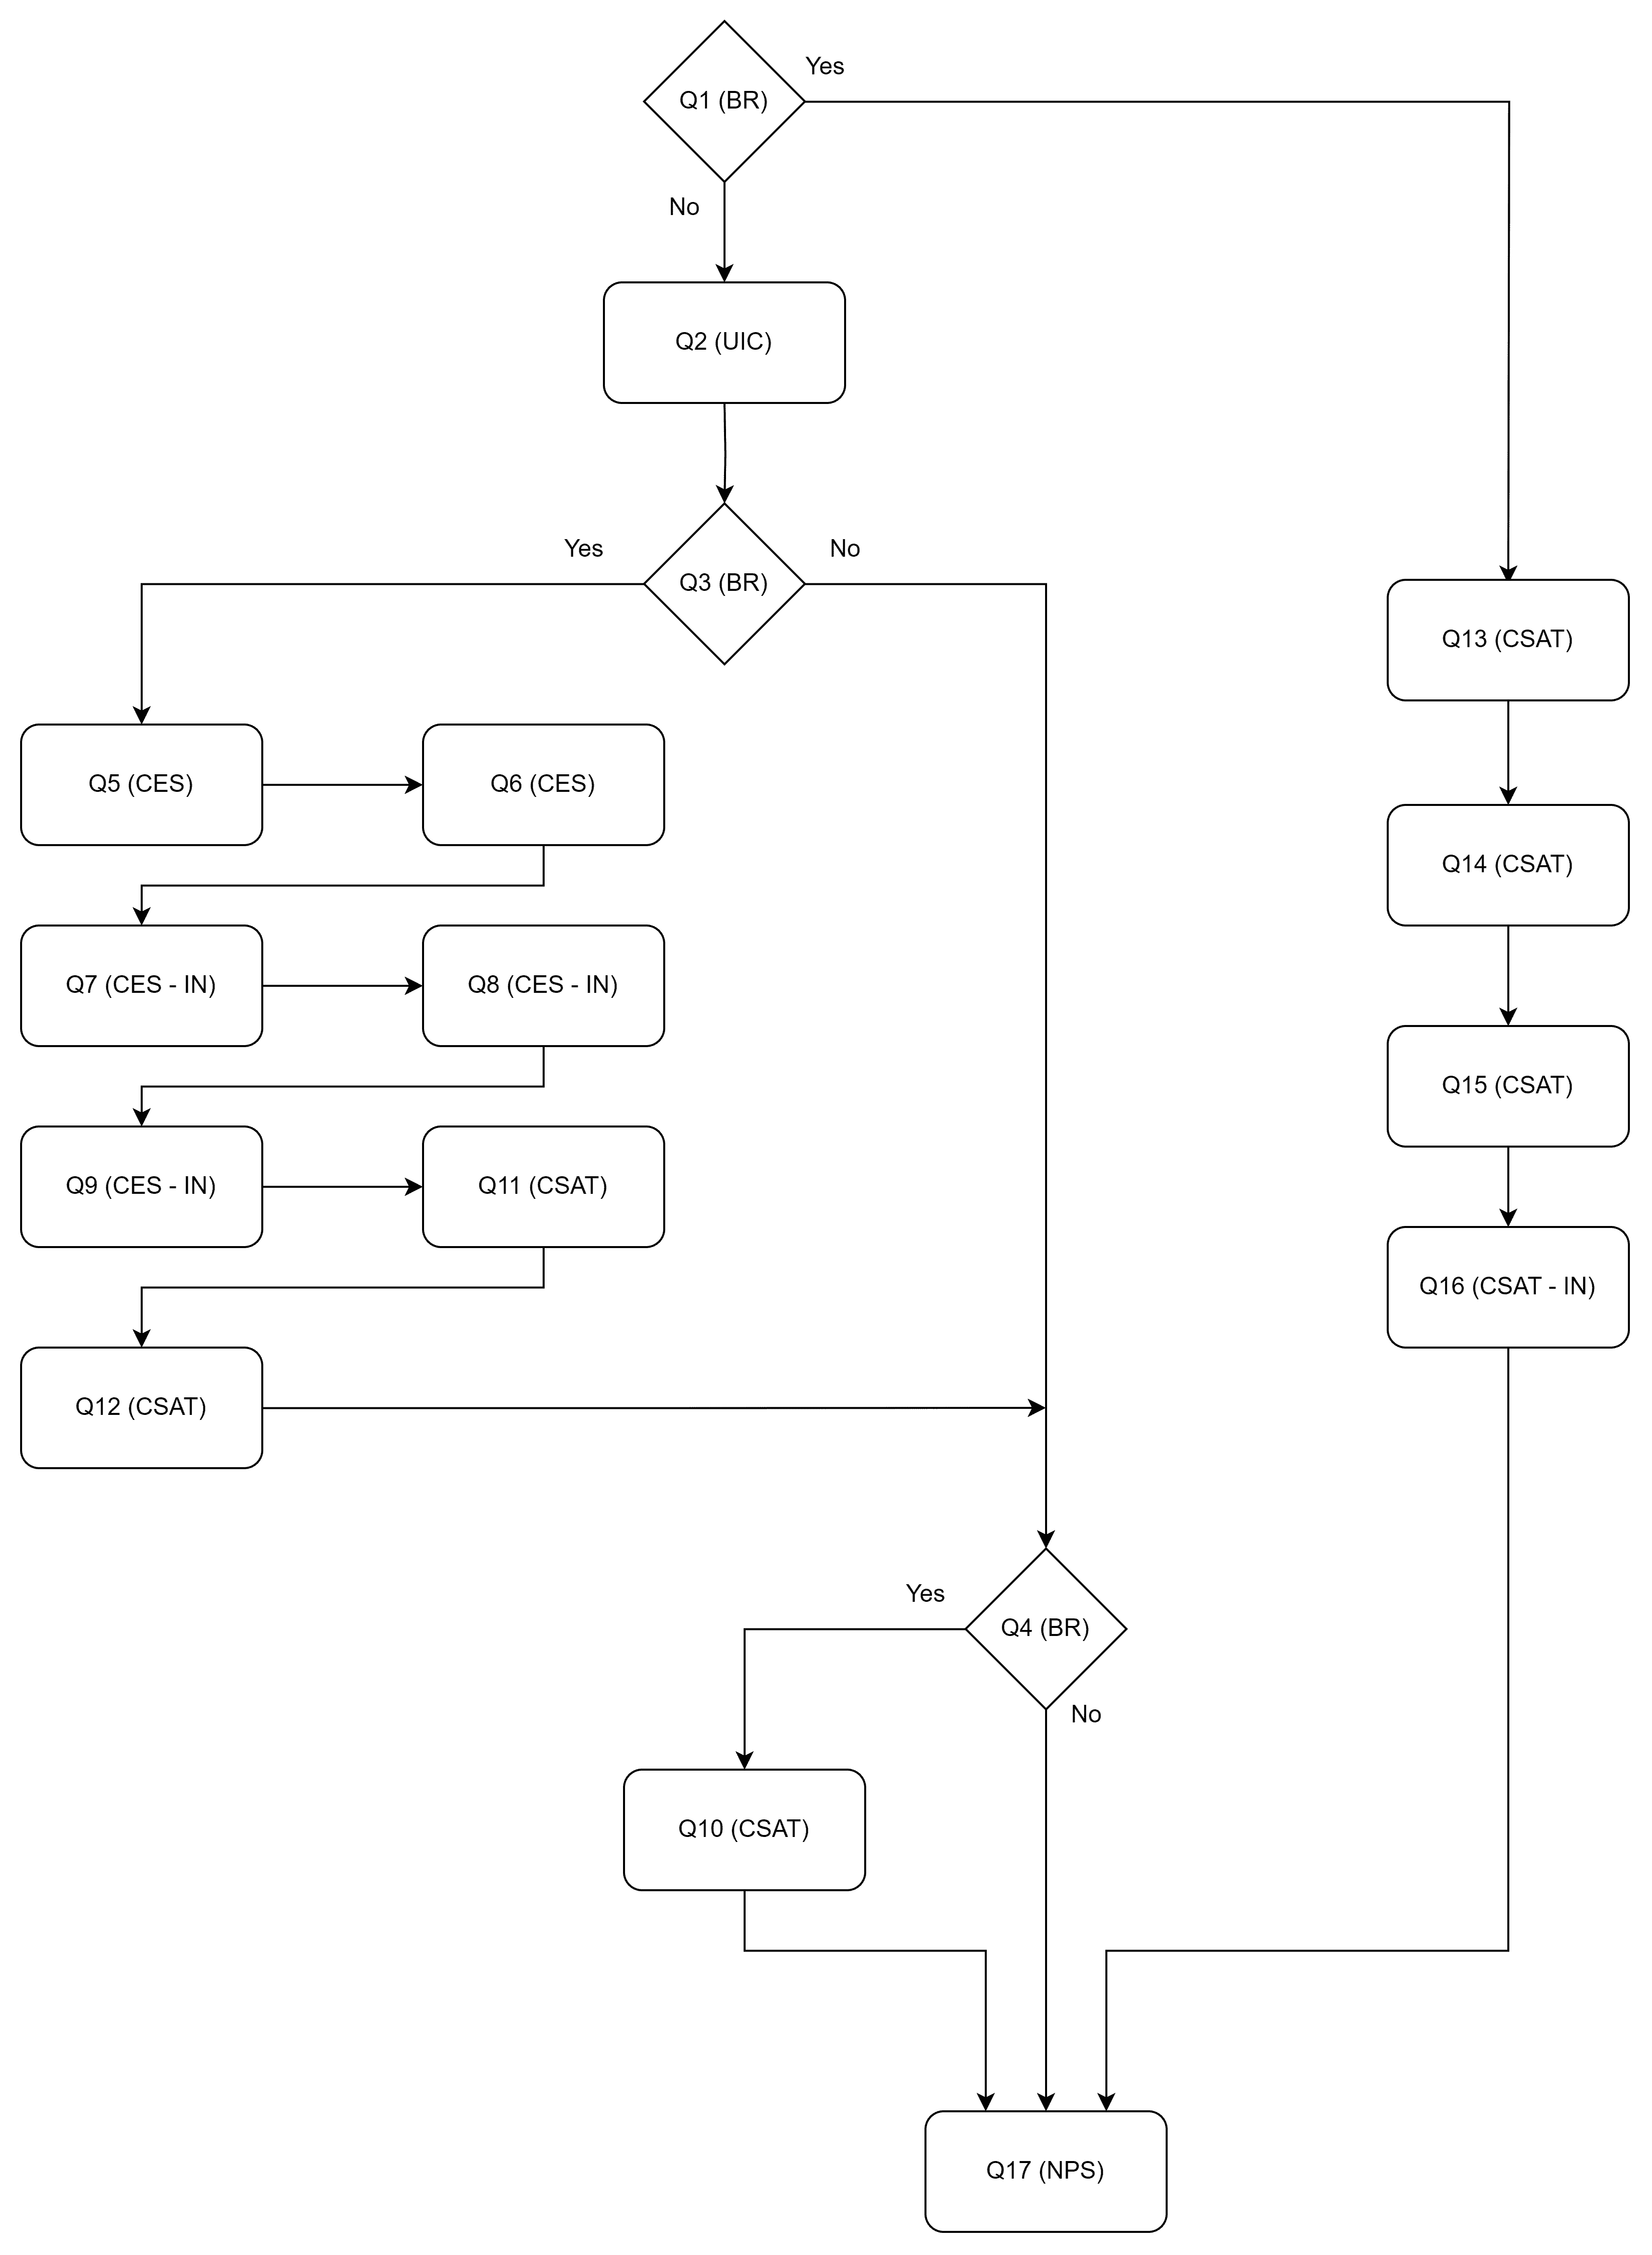
\includegraphics[width = \linewidth]{Content/Cơ sở lý thuyết/documents/Survey/images/surveyflow.png}
        \vspace{0.5cm}
        \caption{Trình tự câu hỏi trong bảng khảo sát}
        \label{fig:Trình tự câu hỏi trong bảng khảo sát}
    \end{figure}
\newpage
\chapter{Phân tích và thiết kế hệ thống}
\subsection{Giới thiệu hệ thống}
Ở đề tài trước, hệ thống (tạm gọi là phiên bản 1.0) đã được hiện thực với một số tính năng quan trọng, chẳng hạn như: thiết kế, so sánh, mô phỏng và đánh giá mô hình BPMN. Ngoài việc cung cấp bộ công cụ đầy đủ các thành phần BPMN 2.0, phiên bản 1.0 này của hệ thống còn hỗ trợ nhập xuất file BPMN, ghi chú trên các thành phần và mô hình, các tính năng undo, redo, zoom-in, zoom-out,... Trong quá trình thiết kế, người dùng cũng có thể xác thực mô hình BPMN về mặt ngữ nghĩa cũng như so sánh các phiên bản khác nhau của mô hình.
\newline
Nhóm chúng tôi nhận ra rằng tính năng quản lý mô hình BPMN của người dùng vẫn chưa được chú trọng. Các dự án của người dùng chỉ mới được đóng gói trong các đơn vị gọi là Project, và chỉ mới thuộc về riêng một cá nhân sở hữu project đó. Tuy nhiên, khi hệ thống được mở rộng, đồng nghĩa với việc số lượng người dùng tăng lên, người ta sẽ có xu hướng nhóm các dự án lại với nhau thành từng cụm lớn hơn. Trong những cụm đó, những người dùng có thể làm việc với nhau trên các project bên trong mỗi cụm, giúp phân tách và quản lý dự án hiệu quả hơn. Chúng tôi gọi đó là tính năng Workspace.
\newline
Workspace được cụ thể hoá bởi các nhóm tính năng chính sau đây:
\begin{itemize}
    \item Quản lý thành viên (members management). Một Workspace có thể có một hoặc nhiều
          người cùng tham gia. Mỗi người dùng đều có một Workspace cá nhân của bản thân,
          gọi là Personal Workspace. Personal Workspace là riêng tư, nên không thể mời
          người khác tham gia vào Personal Workspace của bản thân. Người dùng có thể tự
          tạo Workspace khác (tạm gọi là Regular Workspace) để có thể làm việc với nhiều
          người cho các dự án ở trong Workspace đó. Chủ sở hữu Workspace có thể mời người
          khác tham gia vào Workspace của mình, cũng như thiết lập một số quyền hạn truy
          cập của thành viên, hay loại bỏ thành viên ra khỏi Workspace.
    \item Quản lý dự án (projects management). Các Projects sẽ được khởi tạo trong
          Workspace, cho phép các thành viên trong Workspace có thể truy cập các project
          liên quan tới Workspace đó. Bất kỳ thành viên nào của Workspace với bất kỳ
          quyền hạn nào cũng có thể tạo project của riêng mình trong các Workspace mà
          mình tham gia, và mời các thành viên khác vào project được tạo để cùng nhau
          phát triển. Các projects cũng có thể bị xoá khỏi Workspace tuỳ theo mục đích và
          nhu cầu.
    \item Quản lý yêu cầu (requests management). Quản lý requests là nhóm các tính năng
          cho phép chủ sở hữu Workspace có thể quản lý được những yêu cầu tham gia vào
          Workspace hay những yêu cầu thay đổi quyền hạn của bản thân thành viên để có
          thêm một số quyền truy cập đối với các dữ liệu trong Workspace. Chủ sở hữu
          Workspace có thể chấp thuận, từ chối hay xoá bỏ những yêu cầu nào từ phía thành
          viên. Khi một request được chấp thuận hay từ chối, sẽ có một thông báo gửi về
          cho đối tượng của request đó. Bên cạnh đó, chủ sở hữu Workspace cũng sẽ nhận
          được các requests theo thời gian thực, ngay khi thành viên gửi đi bất kỳ yêu
          cầu nào.
    \item Cá nhân hoá Workspace. Hệ thống cho phép chủ sở hữu Workspace linh hoạt tuỳ
          chỉnh một số thuộc tính của Workspace như tên, mô tả, hình ảnh đại diện của
          Workspace nhằm tăng trải nghiệm cá nhân và phù hợp với mục đích của Workspace
          đó.
\end{itemize}
Bên cạnh tính năng Workspace, nhóm chúng tôi còn phát triển thêm những tính năng thông báo:
\begin{itemize}
    \item Quản lý các thông báo cá nhân. Mỗi người dùng sẽ có một bảng thông báo tổng hợp
          của riêng mình. Các loại thông báo hiện tại bao gồm: thông báo khi yêu cầu thay đổi quyền hạn của bản thân trong
          Workspace tham gia được chấp thuận hay từ chối, thông báo lời mời tham gia
          Workspace từ một thành viên trong Workspace đó. Người dùng có thể chấp nhận
          hoặc từ chối lời mời này. Bên cạnh đó, người dùng có thể thực thi các thao tác
          xoá, lọc, tìm kiếm, đánh dấu những thông báo quan trọng.
    \item Nhận, gửi thông báo theo thời gian thực. Thông thường, để luôn nhận được thông
          báo mới nhất, người dùng cần phải tải lại trang định kỳ để hệ thống trả về các
          thông báo mới. Tuy nhiên, chúng tôi đã hiện thực tính năng thông báo này
          theo thời gian thực, nghĩa là khi có một thông báo mới, nó sẽ được hiển thị
          đồng thời, ngay lập tức cho người dùng, để họ dù đang làm gì trên hệ thống vẫn
          có thể theo dõi được các yêu cầu thay đổi quyền hạn của mình có được chấp nhận hay chưa, hay nhận
          lời mời tham gia Workspace ngay lập tức. Việc hiện thực theo thời gian thực
          giúp tăng khả năng phản hồi và trải nghiệm của người dùng khi sử dụng hệ thống.
\end{itemize}
\par
Trong giai đoạn tới, dựa trên nền tảng lý thuyết đã được xây dựng ở trên, chúng tôi
sẽ hiện thực bảng khảo sát đánh giá sự hài lòng của khách hàng và người dùng tham gia
thực thi quy trình đối với chất lượng của quy trình nghiệp vụ, từ đó đánh giá lại chất
lượng tổng thể của quy trình. Đồng thời, chúng tôi cũng sẽ phát triển thêm tính năng
giám sát, cải tiến quy trình nghiệp vụ, trực quan hoá mức độ ưu tiên của các quy trình
bên trong tổ chức, hỗ trợ đưa ra quyết định cho sự phát triển của quy trình trong tương lai.
\par
Không những vậy, chúng tôi cũng sẽ hiện thực tính năng Template Suggestions. 
Chúng tôi đang hướng tới việc mở hoá hệ thống, nghĩa là cho phép người dùng có thể 
công khai một số project đến cho cộng đồng để được đóng góp và phát triển thành 
những sản phẩm tiềm năng, tối ưu. Những người dùng khác có thể tham gia phát triển, 
tạo bản sao đem về project cá nhân của họ và đánh giá những dự án chất lượng cao 
nhằm xây dựng tài nguyên các mô hình BPMN và đưa ra các đề xuất phù hợp với nhu 
cầu của người dùng khi họ cần tìm kiếm hay khởi tạo dự án nào trong hệ thống, họ 
có thể tham khảo tới những mẫu mô hình được đánh giá cao đã có sẵn.
\newline

Các yêu cầu phi chức năng cũng là yếu tố quan trọng cần được đánh giá, xem xét.
Các yêu cầu phi chức năng dưới đây được chúng tôi đảm bảo hệ thống có thể thực
hiện được nhằm tối ưu hoá trải nghiệm của người dùng, bên cạnh các yêu cầu phi
chức năng kế thừa từ đề tài trước đó:
\begin{center}
    \begin{tabular}{ |m{3cm}|m{10cm}|}
        \hline
        Performance    & \begin{itemize}
                             \item Đối với màn hình input: tối đa 5 trường dữ liệu, không tính toán dữ liệu phức tạp, không tương tác với hệ thống ngoài, có thể lưu trữ dữ liệu trực
                                   tiếp ngay xuống database, không lưu trữ các tệp nội dung lớn như hình ảnh, video, tập tin quá 3 MB.
                             \item Đối với màn hình output: dữ liệu được truy vấn trực tiếp từ database, hạn chế những câu lệnh truy vấn phức tạp, những truy vấn từ hệ thống ngoài.
                                   Hiển thị tối đa 10 dòng dữ liệu, có độ dài nhỏ hơn 100 ký tự
                         \end{itemize} \\
        \hline
        Usability      & \begin{itemize}
                             \item Tất cả thông tin quan trọng phải được hiển thị trong 1 màn hình (không cần phải
                                   thực hiện thêm thao tác cuộn).
                             \item Giao diện của hệ thống cần có sự nhất quán, về mặt hình ảnh biểu tượng cũng như
                                   vị trí các đối tượng trên màn hình để người dùng làm quen dễ dàng hơn.
                             \item Người dùng có thể thành thạo các thao tác trên màn hình trong 15 phút sử dụng.
                         \end{itemize}                                                                    \\
        \hline
        Supportability & \begin{itemize}
                             \item Hệ thống có thể được sử dụng hiệu quả trên các trình duyệt web (Opera, UC
                                   Browser, Safari, Microsoft Edge, Google Chrome, Samsung Internet Browser).
                             \item Hệ thống không chạy trên các phiên bản trình duyệt quá cũ.
                         \end{itemize}                                                                          \\
        \hline
        Scalability    & \begin{itemize}
            \item Có khả năng tách database trên một server riêng và backend trên một
            server riêng      
        \end{itemize}                                                                                                                                                       \\
        \hline
    \end{tabular}
\end{center}

\subsection{Kiến trúc phần mềm}
Với những nghiệp vụ được đề cập ở trên, chúng tôi quyết định lựa chọn hướng
tiếp cận của kiến trúc đa lớp cho hệ thống của chúng tôi. Kiến trúc đa lớp là
một trong những kiến trúc phổ biến trong các loại kiến trúc phần mềm. Kiến trúc
này ra đời nhằm phân chia các thành phần trong hệ thống, các thành phần cùng
chức năng sẽ được nhóm lại với nhau và phân chia công việc cho từng nhóm để dữ
liệu không bị chồng chéo và lộn xộn. Kiến trúc này phát huy hiệu quả nhất ở cả hệ 
thống nhỏ và lớn, giúp cho việc quản lý code và xử lý lỗi dễ
dàng hơn.
\par
Mặc dù không có quy định cụ thể về số lượng hay kiểu của các lớp, ở những hệ
thống phức tạp hơn có thể có nhiều lớp hơn, đa số các kiến trúc đa lớp gồm có
ba lớp chuẩn (3-tier): \emph{Presentation Layer}, \emph{Business Layer},
\emph{Persistence Layer}. \emph{Presentation layer} có nhiệm vụ chính giao tiếp với
người dùng, gồm các thành phần giao diện và thực hiện các công việc như nhập
liệu, hiển thị dữ liệu, kiểm tra tính đúng đắn của dữ liệu trước khi gọi lớp
\emph{Business layer}. \emph{Business layer} phân ra thành hai nhiệm vụ: thứ
nhất, đây là nơi đáp ứng các yêu cầu thao tác dữ liệu của \emph{Presentation
    layer}, xử lý chính nguồn dữ liệu từ \emph{Presentation layer} trước khi truyền
xuống \emph{Persistence layer} và lưu xuống hệ quản trị cơ sở dữ liệu. \emph{Persistence
    layer} có chức năng giao tiếp với hệ quản trị CSDL như thực hiện các công việc
liên quan đến lưu trữ và truy vấn dữ liệu ( tìm kiếm, thêm, xóa, sửa,…).
\par
Kiến trúc này có một số ưu điểm như sau:
\begin{itemize}
    \item Việc phân chia thành từng lớp giúp cho code được tường minh hơn. Nhờ vào việc
          chia ra từng lớp đảm nhận các chức năng khác nhau và riêng biệt như giao diện,
          xử lý, truy vấn thay vì để tất cả lại một chỗ, nhằm giảm sự kết dính.
    \item Dễ bảo trì khi được phân chia, thì một thành phần của hệ thống sẽ dễ thay đổi.
          Việc thay đổi này có thể được cô lập trong 1 lớp, hoặc ảnh hưởng đến lớp gần
          nhất mà không ảnh hưởng đến cả chương trình.
    \item Dễ phát triển, tái sử dụng: khi chúng ta muốn thêm một chức năng nào đó thì
          việc lập trình theo một mô hình sẽ dễ dàng hơn vì chúng ta đã có chuẩn để tuân
          theo. Và việc sử dụng lại khi có sự thay đổi giữa hai môi trường thì chỉ việc
          thay đổi lại \emph{Presentation layer}.
\end{itemize}

\par
Ngoài kiến trúc đa lớp này, chúng tôi còn tìm hiểu thêm một loại kiến trúc cũng
rất phổ biến hiện nay, đó là Microservices. Theo kiến trúc này, một ứng dụng
được chia thành một bộ các microservice, mỗi microservice thực chất là một
service có thể được triển khai và chạy độc lập. Chúng tách biệt về mặt mã
nguồn, về hoạt động và dữ liệu. Mỗi microservice có nơi chứa dữ liệu của riêng
của nó và chỉ có nó có quyền truy cập vào vùng dữ liệu này. Do các microservice
là độc lập, chúng không giao tiếp trực tiếp với nhau mà qua một thành phần
trung gian được gọi là API gateway. Có thể thấy vai trò của API gateway rất
quan trọng trong mô hình microservice. Nó là điểm đến và đi của mọi yêu cầu hay
phản hồi.
\par
Tính phân tán là đặc trưng của kiến trúc này, vì vậy việc xác định mức độ chi
tiết của từng dịch vụ là chìa khóa để xây dựng một hệ thống tốt. Đò là điều khó
đạt được đối với hệ thống đang phát triển của chúng tôi. Một vấn đề khác với
hướng tiếp cận theo kiến trúc này đó là việc các nghiệp vụ trong hệ thống chúng
tôi liên quan khá chặt chẽ, vì vậy kiến trúc Microservices tỏ ra không phù hợp
với hệ thống của chúng tôi.
\section{Use-case}
\subsection{Lược đồ use-case của hệ thống}

Chi tiết về lược đồ use-case của hệ thống:

\href{https://app.diagrams.net/#G1Myz6UnduM7vZYhCvuX0KpLPWf_OdprEM#%7B%22pageId%22%3A%22aGwoCCFz17a1391KKWEK%22%7D}{Tổng hợp diagram hệ thống BPSky}

\begin{figure}[H]
    \begin{center}
        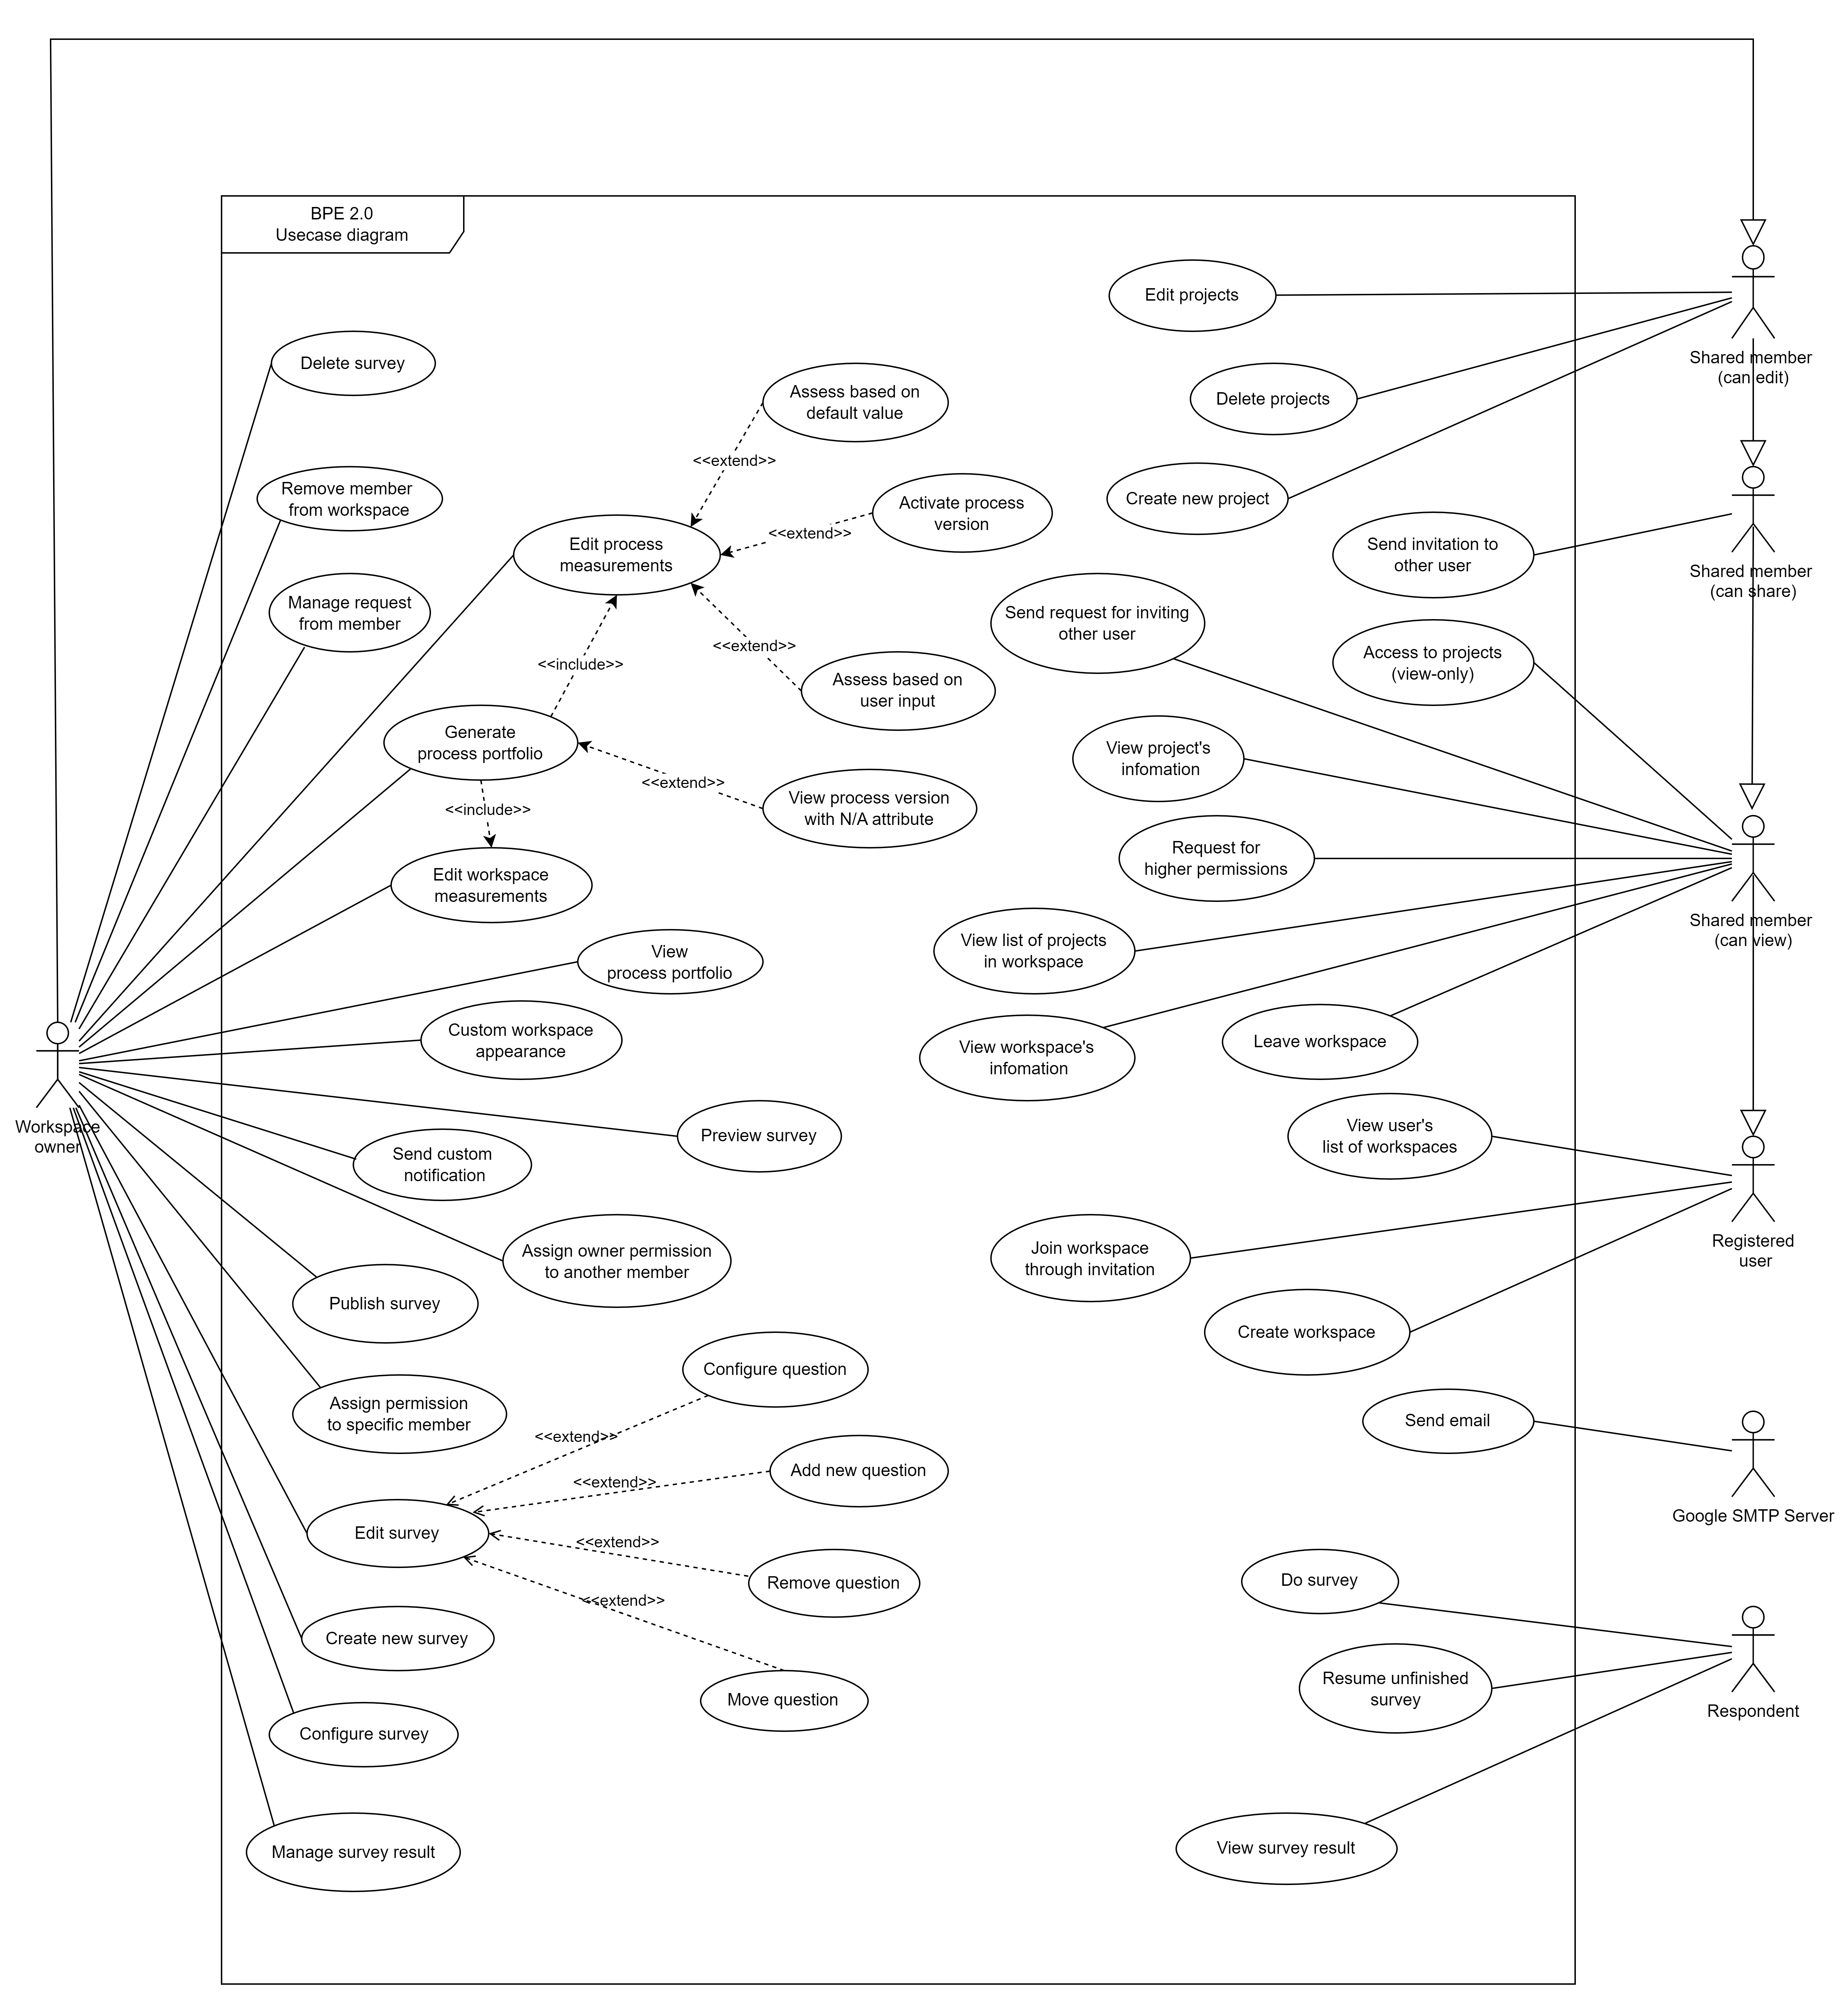
\includegraphics[width=0.85\textwidth]{Content/Phân tích và thiết kế hệ thống/documents/Use case/images/System usecase - HK232.png}
        \vspace{0.5cm}
        \caption{Lược đồ use-case hệ thống}
        \label{fig: Lược đồ use-case hệ thống}
    \end{center}
\end{figure}

% Trang workspace

\subsubsection{Create new workspace}

\begin{table}[H]
\def\arraystretch{2}%
\centering
\resizebox{\textwidth}{!}{%
\begin{tabular}{|p{3cm}|p{11cm}|}
\hline
\textbf{Use-case name}     & Create new workspace
\\ \hline
\textbf{Actor}             & Registered user
\\ \hline
\textbf{Description}       & Người dùng tạo mới workspace
\\ \hline
\textbf{Trigger}           & Không
\\ \hline
\textbf{Pre-conditions}    & Người dùng đã đăng ký vào hệ thống và đăng nhập thành công, hiện tại đang ở giao diện Default homepage
\\ \hline
\textbf{Post-conditions}   & Người dùng tạo mới workspace thành công, và trở thành workspace owner của workspace đó
\\ \hline
\textbf{Normal flow} &
  \begin{enumerate}
      \item Người dùng ở giao diện Default homepage, hiện đang hiển thị danh sách workspace của người dùng đó
      \item Người dùng chọn nút “Create workspace”
      \item Hệ thống mở modal yêu cầu thông tin của workspace: Workspace name, workspace description
      \item Người dùng nhập tên (Name) của workspace
      \item Người dùng nhập mô tả (Description) của workspace
      \item Người dùng chọn nút “Save” để lưu thông tin và hoàn tất tạo mới workspace
  \end{enumerate}
  \\ \hline
\textbf{Alternative flows} & Không
\\ \hline
\textbf{Exceptions} &
  \begin{tabular}{p{10cm}}
      2a. Người dùng chọn nút “Cancel” để đóng modal nhập thông tin workspace
      \\
      3a. Người dùng sử dụng tên của workspace đã tồn tại
      \\ 
      \begin{tabular}{p{9cm}}
          3a.1. Hệ thống yêu cầu người dùng sửa lại tên phù hợp
          \\ 
          3a.2. Tiếp tục bước 4
      \end{tabular}
      \\
      3b. Người dùng không nhập tên của workspace
      \\ 
      \begin{tabular}{p{9cm}}
          3b.1. Hệ thống yêu cầu người dùng phải điền thông tin bắt buộc
          \\ 
          3b.2. Tiếp tục bước 4
      \end{tabular}
  \end{tabular}
  \\ \hline
\end{tabular}
}
\end{table}

\subsubsection{View user’s list of workspaces}

\begin{table}[H]
\def\arraystretch{2}%
\centering
\resizebox{\textwidth}{!}{%
\begin{tabular}{|p{3cm}|p{11cm}|}
\hline
\textbf{Use-case name}     & View user’s list of workspaces
\\ \hline
\textbf{Actor}             & Registered user
\\ \hline
\textbf{Description}       & Xem danh sách những workspaces đã tham gia của người dùng
\\ \hline
\textbf{Trigger}           & Không                                                      \\ \hline
\textbf{Pre-conditions}    & Người dùng đã đăng ký vào hệ thống và đăng nhập thành công \\ \hline
\textbf{Post-conditions}   & Người dùng xem được danh sách những workspaces đã tham gia \\ \hline
\textbf{Normal flow} &
  \begin{enumerate}
      \item Người dùng hiện tại đang ở giao diện Default homepage
      \item Người dùng chọn tab "Recently opened" để xem danh sách những workspace đã tham gia được sắp xếp theo thời gian mở gần nhất
  \end{enumerate}
  \\ \hline
\textbf{Alternative flows} & 2a. Người dùng chọn tab "Pin workspace" để xem danh sách những workspace được ghim
\\ \hline
\textbf{Exceptions}        & Không
\\ \hline
\end{tabular}%
}
\end{table}

\subsubsection{Pin workspace}

\begin{table}[H]
\def\arraystretch{2}%
\centering
\resizebox{\textwidth}{!}{%
\begin{tabular}{|p{3cm}|p{11cm}|}
\hline
\textbf{Use-case name}     & Pin workspace
\\ \hline
\textbf{Actor}             & Registered user
\\ \hline
\textbf{Description}       & Người dùng ghim workspace
\\ \hline
\textbf{Trigger}           & Không
\\ \hline
\textbf{Pre-conditions}    & Người dùng đã đăng ký vào hệ thống và đăng nhập thành công, hiện tại đang ở giao diện Default homepage
\\ \hline
\textbf{Post-conditions}   & Người dùng ghim workspace thành công, và có thể xem những workspace được ghim ở trang Pinned workspace
\\ \hline
\textbf{Normal flow} &
  \begin{enumerate}
      \item Người dùng ở giao diện Default homepage, hiện đang hiển thị danh sách workspace của người dùng đó
      \item Người dùng chọn icon hình ngôi sao ở item workspace tương ứng để ghim workspace
  \end{enumerate}
  \\ \hline
\textbf{Alternative flows} & Không
    2a. Người dùng chọn icon hình ngôi sao ở item workspace tương ứng để bỏ ghim workspace
    \\
    \\ \hline
\textbf{Exceptions} &
    \\ \hline
\end{tabular}
}
\end{table}

\subsubsection{Gửi lời mời đến người dùng khác vào workspace}

\begin{table}[H]
\def\arraystretch{2}%
\centering
\resizebox{\textwidth}{!}{%
\begin{tabular}{|p{3cm}|p{11cm}|}
\hline
\textbf{Use-case name}    & Gửi lời mời đến người dùng khác vào workspace
\\ \hline
\textbf{Actor}            & Thành viên đã tham gia vào workspace
\\ \hline
\textbf{Description}      & Người dùng gửi lời mời tham gia workspace cho người dùng trong hệ thống. 
\\ \hline
\textbf{Trigger}          & Không
\\ \hline
\textbf{Pre-conditions}   & Người dùng đã đăng nhập vào hệ thống thành công
\\ \hline
\textbf{Post-conditions}  & Gửi lời mời người dùng trong hệ thống vào workspace thành công.
\\ \hline
\textbf{Normal Flow} &
    \begin{enumerate}
        \item Người dùng ở giao diện Default homepage, hệ thống hiển thị danh sách những workspace mà người dùng tham gia/sở hữu
        \item Người dùng chọn icon "Menu" ở workspace mà người dùng tham gia với quyền hạn của viewer để hiển thị dropdown menu
        \item Người dùng chọn nút “Share” để hiện modal chia sẻ workspace:
        \begin{enumerate}
            \item Những người hiện có trong workspace
            \item Quyền hạn của những người hiện có trong workspace
        \end{enumerate}
        \item Người dùng nhập email của người được mời để tìm kiếm người dùng trong hệ thống
        \item Người dùng chọn quyền hạn của người dùng được mời vào workspace
        \item Người dùng chọn “Send” để gửi lời mời tới người dùng
    \end{enumerate}
 \\ \hline
\textbf{Alternative flows} &
  \begin{tabular}{p{10cm}}
  4a. Email của người được mời không tồn tại trên hệ thống
    \begin{tabular}{p{9cm}}
          4a.1. Hệ thống hiển thị không tìm thấy kết quả phù hợp
    \end{tabular}
  \\
  5a. Người dùng gán quyền hạn cho người được mời vào workspace vượt quá quyền hạn hiện có trong workspace
      \begin{tabular}{p{9cm}}
          5a.1. Hệ thống thông báo lỗi yêu cầu người dùng gán quyền cho người được mời không vượt quá quyền hạn hiện có (Editor > Sharer > Viewer)
          \\
          5a.2. Tiếp tục ở bước 5
      \end{tabular}
  \\
  \end{tabular} 
\\ \hline
\textbf{Exceptions} &
  \begin{tabular}{p{10cm}}
    5a. Người dùng chọn “Cancel” để hủy yêu cầu và đóng modal
  \end{tabular}
\\ \hline
\end{tabular}%
}
\caption{Use-case scenario cho use-case Gửi lời mời đến người dùng khác vào workspace}
\end{table}

\subsubsection{Gửi yêu cầu mời người dùng khác vào workspace}

\begin{table}[H]
\def\arraystretch{2}%
\centering
\resizebox{\textwidth}{!}{%
\begin{tabular}{|p{3cm}|p{11cm}|}
\hline
\textbf{Use-case name} & Gửi yêu cầu mời người dùng khác vào workspace
\\ \hline
\textbf{Actor} & Workspace member
\\ \hline
\textbf{Description} & Gửi yêu cầu “Chia sẻ workspace đến người khác” tới workspace owner để được xét duyệt
\\ \hline
\textbf{Trigger} & Không 
\\ \hline
\textbf{Pre-conditions} & Người dùng đã đăng ký vào hệ thống và đăng nhập thành công
\\ \hline
\textbf{Post-conditions} & Người dùng gửi thành công yêu cầu “Chia sẻ workspace đến người khác” tới workspace owner để được xét duyệt 
\\ \hline
\textbf{Normal flow} &
  \begin{enumerate}
      \item Người dùng ở giao diện Default homepage, hệ thống hiển thị danh sách những workspace mà người dùng tham gia/sở hữu
      \item Người dùng chọn icon "Menu" ở workspace mà người dùng tham gia với quyền hạn của viewer để hiển thị dropdown menu
      \item Người dùng chọn nút “Share” để hiện modal chia sẻ workspace:
      \begin{enumerate}
          \item Những người hiện có trong workspace
          \item Quyền hạn của những người hiện có trong workspace
      \end{enumerate}
      \item Người dùng nhập email của người được mời để tìm kiếm người dùng trong hệ thống
      \item Người dùng chọn quyền hạn của người dùng được mời vào workspace
      \item Người dùng chọn “Send” để gửi yêu cầu đến workspace owner
  \end{enumerate}
\\ \hline
\textbf{Alternative flows} &
  \begin{tabular}{p{10cm}}
  4a. Email của người được mời không tồn tại trên hệ thống
    \begin{tabular}{p{9cm}}
          4a.1. Hệ thống hiển thị không tìm thấy kết quả phù hợp
    \end{tabular}
  \\
  5a. Người dùng gán quyền hạn cho người được mời vào workspace vượt quá quyền hạn hiện có trong workspace
      \begin{tabular}{p{9cm}}
          5a.1. Hệ thống thông báo lỗi yêu cầu người dùng gán quyền cho người được mời không vượt quá quyền hạn hiện có (Editor > Sharer > Viewer)
          \\
          5a.2. Tiếp tục ở bước 5
      \end{tabular}
  \\
  \end{tabular} 
\\ \hline
\textbf{Exceptions} &
  \begin{tabular}{p{10cm}}
    5a. Người dùng chọn “Cancel” để hủy yêu cầu và đóng modal
  \end{tabular}
\\ \hline
\end{tabular}%
}
\caption{Use-case scenario cho use-case Gửi yêu cầu mời người dùng khác vào workspace}
\end{table}

\subsection{Gửi yêu cầu điều chỉnh quyền hạn trong workspace}

\begin{table}[H]
\def\arraystretch{0.5}%
\centering
\resizebox{\textwidth}{!}{%
\fontsize{11}{13}\selectfont
\begin{tabular}{|p{3cm}|p{11cm}|}
\hline
\textbf{Use-case name} &
  Gửi yêu cầu điều chỉnh quyền hạn trong workspace
\\ \hline
\textbf{Actor} &
  Thành viên đã tham gia vào workspace
\\ \hline
\textbf{Description} &
  Gửi yêu cầu “Cung cấp thêm quyền” tới workspace owner để được xét duyệt 
\\ \hline
\textbf{Trigger} &
  Không
\\ \hline
\textbf{Pre-conditions} &
  Người dùng đã đăng ký vào hệ thống và đăng nhập thành công
\\ \hline
\textbf{Post-conditions} &
  Người dùng gửi thành công yêu cầu “Cung cấp điều chỉnh quyền” tới workspace owner để được xét duyệt 
\\ \hline
\textbf{Normal flow} &
\begin{tabular}{p{10.5cm}}
  \begin{enumerate}
      \item Người dùng ở giao diện của workspace đã chọn và đang tham gia vào workspace dưới quyền hạn của viewer hoặc sharer
      \item Người dùng chọn nút “Create new project”, hệ thống hiện modal thông báo:
      \begin{enumerate}
          \item Người dùng không có quyền hạn để chỉnh sửa nội dung workspace
          \item Gửi yêu cầu đến workspace owner để điều chỉnh quyền trong workspace
      \end{enumerate}
      \item Người dùng chọn nút “Send” để gửi yêu cầu
  \end{enumerate}
\end{tabular}
\\ \hline
\textbf{Alternative flows} &
  Không 
\\ \hline
\textbf{Exceptions} &
  \begin{tabular}{p{10.5cm}}
      3a. Người dùng chọn “Cancel” để đóng modal
  \end{tabular} 
\\ \hline
\end{tabular}%
}
\caption{Use-case scenario cho use-case Gửi yêu cầu điều chỉnh quyền hạn trong workspace}
\end{table}

% Trang notification

\subsubsection{Hiển thị thông báo của người dùng}

\begin{table}[H]
\def\arraystretch{2}%
\centering
\resizebox{\textwidth}{!}{%
\begin{tabular}{|p{3cm}|p{11cm}|}
\hline
\textbf{Use-case name}     & Hiển thị thông báo của người dùng               
\\ \hline
\textbf{Actor}             & Người dùng có tài khoản trong hệ thống
\\ \hline
\textbf{Description}       & Truy cập vào trang thông báo cá nhân
\\ \hline
\textbf{Trigger}           & Không                                               
\\ \hline
\textbf{Pre-conditions}    & Người dùng đã đăng ký vào hệ thống và đăng nhập thành công, hiện tại đang ở giao diện Default homepage
\\ \hline
\textbf{Post-conditions}   & Người dùng truy cập được nội dung trang thông báo cá nhân
\\ \hline
\textbf{Normal flow}       &
  \begin{enumerate}
      \item Người dùng ở giao diện Default homepage
      \item Người dùng chọn icon hình chuông ở thanh điều hướng (navigation bar) để hệ thống điều hướng tới trang thông báo cá nhân
  \end{enumerate}
\\ \hline
\textbf{Alternative flows} & Không
\\ \hline
\textbf{Exceptions}        & Không
\\ \hline
\end{tabular}%
}
\caption{Use-case scenario cho use-case Hiển thị thông báo của người dùng}
\end{table}

\subsubsection{View notification detail}

\begin{table}[H]
\def\arraystretch{2}%
\centering
\resizebox{\textwidth}{!}{%
\begin{tabular}{|p{3cm}|p{11cm}|}
\hline
\textbf{Use-case name}     & View notification detail               
\\ \hline
\textbf{Actor}             & Registered user                  
\\ \hline
\textbf{Description}       & Xem thông tin chi tiết của thông báo người dùng
\\ \hline
\textbf{Trigger}           & Không                                               
\\ \hline
\textbf{Pre-conditions}    & Người dùng đã đăng ký vào hệ thống và đăng nhập thành công, hiện tại đang ở trang thông báo
\\ \hline
\textbf{Post-conditions}   & Người dùng truy cập được nội dung chi tiết của thông báo
\\ \hline
\textbf{Normal flow}       &
  \begin{enumerate}
      \item Người dùng ở trang thông báo và hệ thống hiển thị danh sách thông báo của người dùng
      \item Người dùng chọn item thông báo tương ứng
      \item Hệ thống mở modal hiển thị thông tin chi tiết của thông báo
  \end{enumerate}
\\ \hline
\textbf{Alternative flows} & Không
\\ \hline
\textbf{Exceptions}        & Không
\\ \hline
\end{tabular}%
}
\end{table}

\subsubsection{Ghim thông báo của người dùng}

\begin{table}[H]
\def\arraystretch{2}%
\centering
\resizebox{\textwidth}{!}{%
\begin{tabular}{|p{3cm}|p{11cm}|}
\hline
\textbf{Use-case name}     & Ghim thông báo của người dùng
\\ \hline
\textbf{Actor}             & Người dùng có tài khoản trong hệ thống
\\ \hline
\textbf{Description}       & Người dùng ghim thông báo
\\ \hline
\textbf{Trigger}           & Không
\\ \hline
\textbf{Pre-conditions}    & Người dùng đã đăng ký vào hệ thống và đăng nhập thành công, hiện tại đang ở trang thông báo cá nhân
\\ \hline
\textbf{Post-conditions}   & Người dùng ghim thông báo thành công, và có thể xem những thông báo được ghim thông qua bộ lọc
\\ \hline
\textbf{Normal flow} &
  \begin{enumerate}
      \item Người dùng ở trang thông báo cá nhân, hiện đang hiển thị danh sách thông báo của người dùng đó
      \item Người dùng chọn icon hình ngôi sao ở item thông báo tương ứng để ghim thông báo
  \end{enumerate}
  \\ \hline
\textbf{Alternative flows} &
    2a. Người dùng chọn icon hình ngôi sao ở item thông báo đã được ghim để bỏ ghim thông báo
    \\ \hline
\textbf{Exceptions} & Không
    \\ \hline
\end{tabular}
}
\caption{Use-case scenario cho use-case Ghim thông báo của người dùng}
\end{table}

\subsubsection{Delete notification}

\begin{table}[H]
\def\arraystretch{2}%
\centering
\resizebox{\textwidth}{!}{%
\begin{tabular}{|p{3cm}|p{11cm}|}
\hline
\textbf{Use-case name} & Delete notification. 
\\ \hline
\textbf{Actor} & Registered user
\\ \hline
\textbf{Description} & Người dùng có thể xóa thông báo
\\ \hline
\textbf{Trigger} & Không 
\\ \hline
\textbf{Pre-conditions} & Người dùng đã đăng nhập vào hệ thống và đang ở trang thông báo
\\ \hline
\textbf{Post-conditions} & Xóa thông báo thành công 
\\ \hline
\textbf{Normal Flow} &
    \begin{enumerate}
        \item Người dùng hiện tại đang ở trang thông báo và hệ thống hiển thị danh sách thông báo.
        \item Người dùng chọn vào icon "Menu" của item thông báo, hệ thống hiển thị danh sách menu thao tác với thông báo
        \item Người dùng chọn nút "Delete" trong menu
        \item Hệ thống hiển thị modal yêu cầu người dùng xác nhận xóa thông báo
        \item Người dùng nhấn nút “Delete” để xác nhận xóa thông báo
    \end{enumerate}
\\ \hline
\textbf{Alternative Flow} & Không 
\\ \hline
\textbf{Exceptions} &
  \begin{tabular}{p{10cm}}
        5a. Người dùng chọn "Cancel" để hủy thao tác xóa thông báo
  \end{tabular}
\\ \hline
\end{tabular}%
}
\end{table}

\subsection{Tham gia workspace thông qua lời mời}

\begin{table}[H]
\def\arraystretch{2}%
\centering
\resizebox{\textwidth}{!}{%
\begin{tabular}{|p{3cm}|p{11cm}|}
\hline
\textbf{Use-case name}     & Tham gia workspace thông qua lời mời
\\ \hline
\textbf{Actor}             & Người dùng có tài khoản trong hệ thống
\\ \hline
\textbf{Description}       & Tham gia workspace thông qua “Lời mời tham gia workspace”
\\ \hline
\textbf{Trigger}           &
  \begin{enumerate}
      \item Thành viên trong workspace với quyền Chia sẻ hoặc cao hơn gửi lời mời trực tiếp đến người dùng trên hệ thống và chưa tồn tại trong workspace
      \item Workspace owner đồng ý xét duyệt yêu cầu chia sẻ của thành viên không có quyền Chia sẻ trong workspace đến người dùng trên hệ thống
      \item Workspace owner gửi lời mời tham gia trực tiếp đến người dùng trên hệ thống
  \end{enumerate}
\\ \hline
\textbf{Pre-conditions}    & Người dùng đã đăng ký vào hệ thống và đăng nhập thành công
\\ \hline
\textbf{Post-conditions}   & Người dùng thành công tham gia vào workspace
\\ \hline
\textbf{Normal flow}       &
  \begin{enumerate}
      \item Người dùng chọn icon “Notification” trên thanh điều hướng (navigation bar)
      \item Hệ thống chuyển hướng đến trang Notification (thông báo) của người dùng
      \item Hệ thống hiển thị danh sách những thông báo của người dùng
      \item Người dùng chọn vào thông báo “Lời mời tham gia workspace” để mở modal hiển thị thông tin chi tiết của Lời mời
      \item Người dùng chọn “Accept” để chấp nhận lời mời tham gia vào workspace
  \end{enumerate}
\\ \hline
\textbf{Alternative flows} & 6a. Người dùng chọn “Decline” để từ chối lời mời tham gia workspace
\\ \hline
\textbf{Exceptions}        & 
    \begin{tabular}{p{10cm}}
    6a. Người dùng chọn “Accept” với những lời mời đã hết hiệu lực
    \\
        \begin{tabular}{p{9cm}}
            6a.1. Hệ thống hiển thị lỗi khi xử lý yêu cầu của người dùng
            \\
            6a.2. Hệ thống đóng modal hiển thị thông tin Lời mời vào workspace
        \end{tabular}
    \end{tabular}
\\ \hline
\end{tabular}%
}
\caption{Use-case scenario cho use-case Tham gia workspace thông qua lời mời}
\end{table}

% Trang quản lý

\subsection{Truy cập giao diện quản lý thành viên trong workspace}

\begin{table}[H]
\def\arraystretch{2}%
\centering
\resizebox{\textwidth}{!}{%
\begin{tabular}{|p{3cm}|p{11cm}|}
\hline
\textbf{Use-case name}     & Truy cập trang quản lý thành viên trong workspace                                              
\\ \hline
\textbf{Actor}             & Người sở hữu workspace
\\ \hline
\textbf{Description}       & Truy cập vào trang quản lý thành viên trong workspace của chủ sở hữu workspace
\\ \hline
\textbf{Trigger}           & Không                                                                         \\ \hline
\textbf{Pre-conditions}    & Người dùng đã đăng ký vào hệ thống và đăng nhập thành công, hiện tại đang đứng ở giao diện workspace đã chọn 
\\ \hline
\textbf{Post-conditions}   & Người dùng truy cập vào trang quản lý thành viên của Workspace mà họ sở hữu
\\ \hline
\textbf{Normal flow} &
  \begin{enumerate}
      \item Người dùng ở giao diện workspace đã chọn
      \item Người dùng chọn icon hình bánh răng ở bên cạnh tiêu đề workspace
      \item Hệ thống điều hướng người dùng tới giao diện quản lý, giao diện mặc định là quản lý người dùng trong workspace
  \end{enumerate}
  \\ \hline
\textbf{Alternative flows} & Không
\\ \hline
\textbf{Exceptions}        & Không                                                                         \\ \hline
\end{tabular}%
}
\caption{Use-case scenario cho use-case Truy cập trang quản lý thành viên trong workspace}
\end{table}

\subsection{Truy cập giao diện quản lý yêu cầu từ người dùng trong workspace}

\begin{table}[H]
\def\arraystretch{2}%
\centering
\resizebox{\textwidth}{!}{%
\begin{tabular}{|p{3cm}|p{11cm}|}
\hline
\textbf{Use-case name}     & Truy cập giao diện quản lý yêu cầu từ người dùng trong workspace                                              
\\ \hline
\textbf{Actor}             & Người sở hữu workspace
\\ \hline
\textbf{Description}       & Truy cập vào trang quản lý yêu cầu của chủ sở hữu Workspace
\\ \hline
\textbf{Trigger}           & Không                                                                         \\ \hline
\textbf{Pre-conditions} &
  Người dùng đã đăng ký vào hệ thống và đăng nhập thành công, hiện tại đang đứng ở giao diện workspace đã chọn \\ \hline
\textbf{Post-conditions}   & Người dùng truy cập vào trang quản lý yêu cầu của Workspace mà họ sở hữu
\\ \hline
\textbf{Normal flow} &
  \begin{enumerate}
      \item Người dùng ở giao diện workspace đã chọn
      \item Người dùng chọn icon hình bánh răng ở bên cạnh tiêu đề workspace
      \item Hệ thống điều hướng người dùng tới giao diện quản lý, giao diện mặc định là quản lý người dùng
      \item Người dùng chọn tab "Requests management" ở thanh sidebar
      \item Hệ thống điều hướng người dùng tới giao diện quản lý yêu cầu của workspace
  \end{enumerate}
  \\ \hline
\textbf{Alternative flows} & Không                                                                         \\ \hline
\textbf{Exceptions}        & Không                                                                         \\ \hline
\end{tabular}%
}
\caption{Use-case scenario cho use-case Truy cập giao diện quản lý yêu cầu từ người dùng trong workspace}
\end{table}

\subsection{Xét duyệt yêu cầu từ phía người dùng}

\begin{table}[H]
\def\arraystretch{2}%
\centering
\resizebox{\textwidth}{!}{%
\begin{tabular}{|p{3cm}|p{11cm}|}
\hline
\textbf{Use-case name}   & Xét duyệt yêu cầu từ phía người dùng
\\ \hline
\textbf{Actor}           & Người sở hữu workspace
\\ \hline
\textbf{Description}     & Người sở hữu workspace xét duyệt các yêu cầu từ thành viên trong Workspace 
\\ \hline
\textbf{Trigger}         & Không
\\ \hline
\textbf{Pre-conditions}  & Người dùng đã đăng nhập vào hệ thống, người dùng hiện tại đang ở giao diện workspace mà người dùng sở hữu
\\ \hline
\textbf{Post-conditions} & Thành công xét duyệt các yêu cầu từ người dùng trong workspace
\\ \hline
\textbf{Normal Flow}     &
    \begin{enumerate}
        \item Người dùng chọn icon hình bánh răng bên cạnh tiêu đề workspace, hệ thống chuyển hướng đến trang quản lý workspace. Mặc định ở giao diện "Members management"
        \item Người dùng chọn "Requests management" ở thanh sidebar để hệ thống chuyển hướng tới trang quản lý yêu cầu của workspace.
        \item Hệ thống hiển thị danh sách những yêu cầu từ người dùng trong workspace.
        \item Người dùng chọn vào yêu cầu để mở modal hiển thị những thông tin của yêu cầu.
        \item Người dùng chọn nút "Approve" trong modal để chấp nhận yêu cầu tương ứng.
    \end{enumerate}
\\ \hline
\textbf{Alternative Flow} &
    \begin{tabular}{p{10cm}}
        5a. Người dùng chọn "Decline" trong modal để từ chối yêu cầu tương ứng.
    \end{tabular}
\\ \hline
\textbf{Exceptions}      & 
    \begin{tabular}{p{10cm}}
        5a. Người dùng chọn "Cancel" để hủy thao tác, hệ thống tắt modal xác nhận
    \end{tabular}
\\ \hline
\end{tabular}%
}
\caption{Use-case scenario cho use-case Xét duyệt yêu cầu từ phía người dùng}
\end{table}

\subsection{Xóa yêu cầu từ thành viên trong workspace gửi đến}

\begin{table}[H]
\def\arraystretch{2}%
\centering
\resizebox{\textwidth}{!}{%
\begin{tabular}{|p{3cm}|p{11cm}|}
\hline
\textbf{Use-case name} &  Xóa yêu cầu từ thành viên trong workspace gửi đến
\\ \hline
\textbf{Actor} &  Người sở hữu workspace
\\ \hline
\textbf{Description} &  Người sở hữu workspace yêu cầu của thành viên gửi đến
\\ \hline
\textbf{Trigger} &  Không 
\\ \hline
\textbf{Pre-conditions} &  Người dùng đăng nhập vào hệ thống, người dùng hiện tại đang ở giao diện quản lý yêu cầu của workspace mà người dùng sở hữu
\\ \hline
\textbf{Post-conditions} &  Thành công yêu cầu từ thành viên gửi đến
\\ \hline
\textbf{Normal Flow} &
  \begin{enumerate}
      \item Người dùng đang ở giao diện quản lý yêu cầu của workspace
      \item Hệ thống hiển thị danh sách yêu cầu trong workspace.
      \item Người dùng chọn một hoặc nhiều yêu cầu. Hệ thống hiển thị nút "Delete"
      \item Người dùng chọn nút “Delete”, hệ thống hiển thị modal xác nhận thao tác xóa yêu cầu đã chọn
      \item Người dùng chọn “Delete” để thành công xóa yêu cầu
  \end{enumerate}
\\ \hline
\textbf{Alternative Flow} & Không
\\ \hline
\textbf{Exceptions} &
     \begin{tabular}{p{10cm}}
        5a. Người dùng chọn "Cancel" để tắt modal
     \end{tabular}
\\ \hline
\end{tabular}%
}
\caption{Use-case scenario cho use-case Xóa yêu cầu từ thành viên trong workspace gửi đến}
\end{table}

\subsubsection{Xóa thành viên khỏi workspace}

\begin{table}[H]
\def\arraystretch{2}%
\centering
\resizebox{\textwidth}{!}{%
\begin{tabular}{|p{3cm}|p{11cm}|}
\hline
\textbf{Use-case name} &
  Xóa thành viên khỏi workspace
\\ \hline
\textbf{Actor} &
  Người sở hữu workspace
\\ \hline
\textbf{Description} &
  Người sở hữu workspace xóa thành viên ra khỏi Workspace 
\\ \hline
\textbf{Trigger} &
  Không 
\\ \hline
\textbf{Pre-conditions} &
  Người dùng đăng nhập vào hệ thống, người dùng hiện tại đang ở giao diện workspace mà người dùng sở hữu
\\ \hline
\textbf{Post-conditions} &
  Thành công xóa người dùng khỏi workspace
\\ \hline
\textbf{Normal Flow} &
  \begin{enumerate}
      \item Người dùng chọn icon hình bánh răng bên cạnh tiêu đề workspace, hệ thống chuyển hướng đến trang quản lý workspace. Mặc định ở giao diện "Members management"
      \item Hệ thống hiển thị danh sách thành viên trong workspace.
      \item Người dùng chọn một hoặc nhiều thành viên. Hệ thống hiển thị nút "Delete"
      \item Người dùng chọn nút “Delete”, hệ thống hiển thị modal xác nhận thao tác xóa thành viên đã chọn khỏi workspace
      \item Người dùng chọn “Delete” để loại trừ thành viên khỏi workspace
  \end{enumerate}
  \\ \hline
\textbf{Alternative Flow} &
    \begin{tabular}{p{10cm}}
        3a. Danh sách thành viên chỉ có workspace owner, người dùng không thể lựa chọn thành viên để thao tác
    \end{tabular}
\\ \hline
\textbf{Exceptions} &
     \begin{tabular}{p{10cm}}
        5a. Người dùng chọn "Cancel" để tắt modal
     \end{tabular}
\\ \hline
\end{tabular}%
}
\caption{Use-case scenario cho use-case Xóa thành viên khỏi workspace}
\end{table}

% Trang project (workspace's detail)

\subsubsection{Truy cập vào nội dung trong workspace}

\begin{table}[H]
\def\arraystretch{2}%
\centering
\resizebox{\textwidth}{!}{%
\begin{tabular}{|p{3cm}|p{11cm}|}
\hline
\textbf{Use-case name}     & Truy cập vào nội dung trong workspace               
\\ \hline
\textbf{Actor}             & Người tham gia vào workspace      
\\ \hline
\textbf{Description}       & Truy cập vào nội dung project bên trong workspace
\\ \hline
\textbf{Trigger}           & Không                                               
\\ \hline
\textbf{Pre-conditions}    & Người dùng đã đăng ký vào hệ thống và đăng nhập thành công, hiện tại đang ở giao diện Workspace của workspace được chọn
\\ \hline
\textbf{Post-conditions}   & Người dùng xem nội dung project bên trong workspace được chọn
\\ \hline
\textbf{Normal flow}       &
  \begin{enumerate}
      \item Người dùng ở giao diện Workspace của workspace được chọn
      \item Hệ thống hiển thị cho người dùng xem được danh sách những project bên trong workspace
      \item Người dùng chọn project tương ứng để xem nội dung bên trong dưới dạng danh sách xổ xuống (files, processes, documents,...)
  \end{enumerate}
\\ \hline
\textbf{Alternative flows} & Không
\\ \hline
\textbf{Exceptions}        & Không
\\ \hline
\end{tabular}%
}
\caption{Use-case scenario cho use-case Truy cập vào nội dung trong workspace}
\end{table}

\subsection{Tạo mới project trong workspace}

\begin{table}[H]
\def\arraystretch{2}%
\centering
\resizebox{\textwidth}{!}{%
\begin{tabular}{|p{3cm}|p{11cm}|}
\hline
\textbf{Use-case name}    & Tạo mới project trong workspace
\\ \hline
\textbf{Actor}            & Người tham gia vào workspace có quyền hạn chỉnh sửa
\\ \hline
\textbf{Description}      & Người dùng có thể tạo project trong Workspace 
\\ \hline
\textbf{Trigger}          & Không
\\ \hline
\textbf{Pre-conditions}   & Người dùng đã đăng nhập vào hệ thống, hiện tại đang ở giao diện workspace người dùng muốn tạo project. Người dùng có quyền hạn của editor hoặc owner.
\\ \hline
\textbf{Post-conditions}  & Tạo project thành công
\\ \hline
\textbf{Normal Flow} &
    \begin{enumerate}
        \item Người dùng chọn nút “Create project”
        \item Hệ thống mở modal yêu cầu thông tin của project: project name, project description
        \item Người dùng nhập tên (Name) của project
        \item Người dùng nhập mô tả (Description) của project
        \item Người dùng chọn nút “Save” để lưu thông tin và hoàn tất tạo mới project
    \end{enumerate}
\\ \hline
\textbf{Alternative Flow} & Không
\\ \hline
\textbf{Exceptions} &
   \begin{tabular}{p{10cm}}
      3a. Người dùng chọn nút “Cancel” để đóng modal nhập thông tin workspace
      \\
      4a. Người dùng sử dụng tên của workspace đã tồn tại
      \\ 
      \begin{tabular}{p{9cm}}
          4a.1. Hệ thống yêu cầu người dùng sửa lại tên phù hợp
          \\ 
          4a.2. Tiếp tục bước 4
      \end{tabular}
      \\
      4b. Người dùng không nhập tên của workspace
      \\ 
      \begin{tabular}{p{9cm}}
          4b.1. Hệ thống yêu cầu người dùng phải điền thông tin bắt buộc
          \\ 
          4b.2. Tiếp tục bước 4
      \end{tabular}
  \end{tabular} 
\\ \hline
\end{tabular}%
}
\caption{Use-case scenario cho use-case Tạo mới project trong workspace}
\end{table}

\subsection{Xóa project trong Workspace}

\begin{table}[H]
\def\arraystretch{2}%
\centering
\resizebox{\textwidth}{!}{%
\begin{tabular}{|p{3cm}|p{11cm}|}
\hline
\textbf{Use-case name} & Xóa project trong workspace 
\\ \hline
\textbf{Actor} & Người tham gia vào workspace có quyền hạn chỉnh sửa
\\ \hline
\textbf{Description} & Người dùng có thể xóa project trong Workspace
\\ \hline
\textbf{Trigger} & Không 
\\ \hline
\textbf{Pre-conditions} & Người dùng đã đăng nhập vào hệ thống và đang ở giao diện workspace đã chọn, người dùng có quyền hạn của editor hoặc owner
\\ \hline
\textbf{Post-conditions} & Xóa project thành công 
\\ \hline
\textbf{Normal Flow} &
    \begin{enumerate}
        \item Người dùng hiện tại đang ở giao diện workspace và hệ thống hiển thị danh sách project.
        \item Người dùng chọn vào icon "Menu" của item project, hệ thống hiển thị danh sách menu thao tác với project
        \item Người dùng chọn nút "Delete" trong menu
        \item Hệ thống hiển thị modal yêu cầu người dùng xác nhận xóa project
        \item Người dùng nhấn nút “Delete” để xác nhận xóa project
    \end{enumerate}
\\ \hline
\textbf{Alternative Flow} & Không 
\\ \hline
\textbf{Exceptions} &
  \begin{tabular}{p{10cm}}
        5a. Người dùng chọn "Cancel" để hủy thao tác xóa project
  \end{tabular}
\\ \hline
\end{tabular}%
}
\caption{Use-case scenario cho use-case Xóa project trong Workspace}
\end{table}

% Trang survey

\subsection{Khởi tạo bảng khảo sát}

\begin{table}[H]
\def\arraystretch{2}%
\centering
\resizebox{\textwidth}{!}{%
\begin{tabular}{|p{3cm}|p{11cm}|}
\hline
\textbf{Use-case name}     & Khởi tạo bảng khảo sát                          \\ \hline
\textbf{Actor}             & Người sở hữu Project    \\ \hline
\textbf{Description}       & Người sở hữu Project tạo mới bảng khảo sát                       \\ \hline
\textbf{Trigger}           & Không                                    \\ \hline
\textbf{Pre-conditions} &
  Người dùng đã đăng ký vào hệ thống và đăng nhập thành công, hiện tại đang đứng ở giao diện \textbf{Process Editor} \\ \hline
\textbf{Post-conditions}   & Người dùng khởi tạo bảng khảo sát thành công \\ \hline
\textbf{Normal flow} &
  \begin{enumerate}
      \item Người dùng chọn nút \textbf{Launch survey} trên thanh công cụ.
      \item Hệ thống điều hướng người dùng đến trang quản lý bảng khảo sát, mặc định là trang \textbf{Survey Builder}.
  \end{enumerate}
  \\ \hline
\textbf{Alternative flows} & Không                 \\ \hline
\textbf{Exceptions}        & Không                                    \\ \hline
\end{tabular}%
}
\caption{Use-case scenario cho use-case Khởi tạo bảng khảo sát}
\end{table}

\subsection{Chỉnh sửa nội dung bảng khảo sát}

\begin{table}[H]
\def\arraystretch{2}%
\centering
\resizebox{\textwidth}{!}{%
\begin{tabular}{|p{3cm}|p{11cm}|}
\hline
\textbf{Use-case name}     & Chỉnh sửa bảng khảo sát                          \\ \hline
\textbf{Actor}             & Người sở hữu Project    \\ \hline
\textbf{Description}       & Người sở hữu Project chỉnh sửa bảng khảo sát                       \\ \hline
\textbf{Trigger}           & Không                                    \\ \hline
\textbf{Pre-conditions} &
  Người dùng đã đăng ký vào hệ thống và đăng nhập thành công, hiện tại đang đứng ở giao diện \textbf{Process Editor} \\ \hline
\textbf{Post-conditions}   & Người dùng chỉnh sửa survey thành công \\ \hline
\textbf{Normal flow} &
  \begin{enumerate}
      \item Người dùng chọn nút Launch survey trên thanh công cụ.
      \item Hệ thống điều hướng người dùng đến trang quản lý bảng khảo sát, mặc định là trang \textbf{Survey Builder}
      \item Người dùng thực hiện chỉnh sửa nội dung bảng khảo sát.
      \item Hệ thống tự động lưu lại những thay đổi của người dùng.
  \end{enumerate}
  \\ \hline
\textbf{Alternative flows} & Không                 \\ \hline
\textbf{Exceptions}        & Không                                    \\ \hline
\end{tabular}%
}
\caption{Use-case scenario cho use-case Chỉnh sửa nội dung bảng khảo sát}
\end{table}

\subsection{Tuỳ chỉnh thiết lập bảng khảo sát}

\begin{table}[H]
\def\arraystretch{2}%
\centering
\resizebox{\textwidth}{!}{%
\begin{tabular}{|p{3cm}|p{11cm}|}
\hline
\textbf{Use-case name}     & Tuỳ chỉnh thiết lập bảng khảo sát                          \\ \hline
\textbf{Actor}             & Project owner    \\ \hline
\textbf{Description}       & Tuỳ chỉnh thiết lập bảng khảo sát                      \\ \hline
\textbf{Trigger}           & Không                                    \\ \hline
\textbf{Pre-conditions} &
  Người dùng đã đăng ký vào hệ thống và đăng nhập thành công, hiện tại đang đứng ở giao diện \textbf{Survey Builder} \\ \hline
\textbf{Post-conditions}   & Người dùng chỉnh sửa thiết lập bảng khảo sát thành công \\ \hline
\textbf{Normal flow} &
  \begin{enumerate}
      \item Người dùng chọn tab \textbf{Configuration}.
      \item Hệ thống hiển thị trang thiết lập bảng khảo sát.
      \item Người dùng thay đổi các giá trị: thời gian survey bắt đầu\/hết hạn, đóng\/mở survey thủ công, quyền riêng tư của nội dung survey.
      \item Người dùng chọn nút Save changes.
      \item Hệ thống lưu lại thay đổi của người dùng.
  \end{enumerate}
  \\ \hline
\textbf{Alternative flows} & Không                 \\ \hline
\textbf{Exceptions}        & Không                                    \\ \hline
\end{tabular}%
}
\caption{Use-case scenario cho use-case Tuỳ chỉnh thiết lập bảng khảo sát}
\end{table}

\subsection{Quản lý kết quả thực hiện bảng khảo sát}

\begin{table}[H]
\def\arraystretch{2}%
\centering
\resizebox{\textwidth}{!}{%
\begin{tabular}{|p{3cm}|p{11cm}|}
\hline
\textbf{Use-case name}     & Quản lý kết quả thực hiện bảng khảo sát                         \\ \hline
\textbf{Actor}             & Người sở hữu Project    \\ \hline
\textbf{Description}       & Người sở hữu Project quản lý kết quả bảng khảo sát                      \\ \hline
\textbf{Trigger}           & Không                                    \\ \hline
\textbf{Pre-conditions} &
  Người dùng đã đăng ký vào hệ thống và đăng nhập thành công, hiện tại đang đứng ở giao diện \textbf{Survey Builder} \\ \hline
\textbf{Post-conditions}   & Người dùng quản lý kết quả bảng khảo sát thành công \\ \hline
\textbf{Normal flow} &
  \begin{enumerate}
      \item Người dùng chọn tab \textbf{Result}.
      \item Hệ thống hiển thị trang kết quả survey.
      \item Người dùng xem các điểm của survey, số lượng người đã tham gia làm khảo sát, thống kê trả lời mỗi câu hỏi.
  \end{enumerate}
  \\ \hline
\textbf{Alternative flows} & Không                 \\ \hline
\textbf{Exceptions}        & Không                                    \\ \hline
\end{tabular}%
}
\caption{Use-case scenario cho use-case Quản lý kết quả thực hiện bảng khảo sát}
\end{table}

\subsection{Xem trước bảng khảo sát}

\begin{table}[H]
\def\arraystretch{2}%
\centering
\resizebox{\textwidth}{!}{%
\begin{tabular}{|p{3cm}|p{11cm}|}
\hline
\textbf{Use-case name}     & Xem trước bảng khảo sát                          \\ \hline
\textbf{Actor}             & Người sở hữu Project    \\ \hline
\textbf{Description}       & Người sở hữu Project xem trước bảng khảo sát trước khi công bố                      \\ \hline
\textbf{Trigger}           & Không                                    \\ \hline
\textbf{Pre-conditions} &
  Người dùng đã đăng ký vào hệ thống và đăng nhập thành công, hiện tại đang đứng ở giao diện \textbf{Survey Builder} \\ \hline
\textbf{Post-conditions}   & Người dùng xem trước bảng khảo sát thành công \\ \hline
\textbf{Normal flow} &
  \begin{enumerate}
      \item Người dùng chọn nút Preview.
      \item Hệ thống hiển thị giao diện survey sẽ được publish cho người khác.
  \end{enumerate}
  \\ \hline
\textbf{Alternative flows} & Không                 \\ \hline
\textbf{Exceptions}        & Không                                    \\ \hline
\end{tabular}%
}
\caption{Use-case scenario cho use-case Xem trước bảng khảo sát}
\end{table}

\subsection{Công bố bảng khảo sát}

\begin{table}[H]
\def\arraystretch{2}%
\centering
\resizebox{\textwidth}{!}{%
\begin{tabular}{|p{3cm}|p{11cm}|}
\hline
\textbf{Use-case name}     & Công bố bảng khảo sát                         \\ \hline
\textbf{Actor}             & Người sở hữu Project    \\ \hline
\textbf{Description}       & Người sở hữu Project công bố bảng khảo sát                      \\ \hline
\textbf{Trigger}           & Không                                    \\ \hline
\textbf{Pre-conditions} &
  Người dùng đã đăng ký vào hệ thống và đăng nhập thành công, hiện tại đang đứng ở giao diện \textbf{Survey Builder} \\ \hline
\textbf{Post-conditions}   & Người dùng công bố bảng khảo sát thành công \\ \hline
\textbf{Normal flow} &
  \begin{enumerate}
      \item Người dùng chọn nút \textbf{Publish}.
      \item Hệ thống hiển thị modal.
      \item Người dùng nhập email cần được gửi bảng khảo sát tới.
      \item Người dùng chọn biểu tượng dấu cộng để thêm email vào danh sách cần gửi.
      \item Hệ thống hiển thị những email đã được thêm vào ở bên dưới ô nhập email.
      \item Người dùng chọn ngày giờ bắt đầu và kết thúc bảng khảo sát.
      \item Người dùng chọn nút \textbf{Publish}.
      \item Survey được chuyển sang trạng thái pending. Dựa vào thời gian được thiết lập, hệ thống gửi email tới những người có trong danh sách, sau đó survey được chuyển sang trạng thái published.
  \end{enumerate}
  \\ \hline
\textbf{Alternative flows} &
    \begin{tabular}{p{10cm}}
        Người dùng công bố ngay lập tức. \\
        6a. Người dùng chọn nút Publish sau khi modal được hiển thị. \\
        7a. Hệ thống gửi email ngay lập tức nếu có, survey được chuyển sang trạng thái published.
    \end{tabular}             \\ \hline
\textbf{Exceptions}        & 
    \begin{tabular}{p{10cm}}
        3c. Người dùng chọn nút Cancel. \\
        4c. Hệ thống tắt cửa sổ popup. \\ 
        Usecase kết thúc.
    \end{tabular}                                    \\ \hline
\end{tabular}%
}
\caption{Use-case scenario cho use-case Công bố bảng khảo sát}
\end{table}

\subsection{Thêm câu hỏi mới}

\begin{table}[H]
\def\arraystretch{2}%
\centering
\resizebox{\textwidth}{!}{%
\begin{tabular}{|p{3cm}|p{11cm}|}
\hline
\textbf{Use-case name}     & Thêm câu hỏi mới                          \\ \hline
\textbf{Actor}             & Người sở hữu Project    \\ \hline
\textbf{Description}       & Người sở hữu Project thêm câu hỏi mới trong bảng khảo sát                      \\ \hline
\textbf{Trigger}           & Không                                    \\ \hline
\textbf{Pre-conditions} &
  Người dùng đã đăng ký vào hệ thống và đăng nhập thành công, hiện tại đang đứng ở giao diện \textbf{Survey Builder} \\ \hline
\textbf{Post-conditions}   & Người dùng thêm câu hỏi thành công \\ \hline
\textbf{Normal flow} &
  \begin{enumerate}
      \item Người dùng chọn nút biểu tượng dấu cộng ở trên hoặc dưới câu hỏi bất kỳ.
      \item Hệ thống hiển thị modal.
      \item Người dùng chỉnh sửa nội dung câu hỏi.
      \item Hệ thống lưu lại những thay đổi của người dùng và tạo câu hỏi mới tại vị trí được chỉ định.
  \end{enumerate}
  \\ \hline
\textbf{Alternative flows} & Không                 \\ \hline
\textbf{Exceptions}        & Không                                    \\ \hline
\end{tabular}%
}
\caption{Use-case scenario cho use-case Thêm câu hỏi mới vào bảng khảo sát}
\end{table}

\subsection{Xoá câu hỏi trong bảng khảo sát}

\begin{table}[H]
\def\arraystretch{2}%
\centering
\resizebox{\textwidth}{!}{%
\begin{tabular}{|p{3cm}|p{11cm}|}
\hline
\textbf{Use-case name}     & Xoá câu hỏi trong bảng khảo sát                          \\ \hline
\textbf{Actor}             & Người sở hữu Project    \\ \hline
\textbf{Description}       & Người sở hữu Project xoá câu hỏi trong bảng khảo sát                      \\ \hline
\textbf{Trigger}           & Không                                    \\ \hline
\textbf{Pre-conditions} &
  Người dùng đã đăng ký vào hệ thống và đăng nhập thành công, hiện tại đang đứng ở giao diện \textbf{Survey Builder} \\ \hline
\textbf{Post-conditions}   & Người dùng xoá câu hỏi thành công \\ \hline
\textbf{Normal flow} &
  \begin{enumerate}
      \item Người dùng chọn nút biểu thị Delete bên cạnh câu hỏi bất kỳ.
      \item Hệ thống hiển thị cảnh báo.
      \item Người dùng chọn nút Delete.
      \item Hệ thống xoá câu hỏi khỏi survey.
  \end{enumerate}
  \\ \hline
\textbf{Alternative flows} & Không                 \\ \hline
\textbf{Exceptions}        & 
  \begin{tabular}{p{10cm}}
        3a. Người dùng chọn nút Cancel. \\ 
        4a. Hệ thống đóng modal, hiển thị lại giao diện chỉnh sửa survey. \\ 
        Usecase kết thúc.
    \end{tabular}                                    \\ \hline
\end{tabular}%
}
\caption{Use-case scenario cho use-case Xoá câu hỏi trong bảng khảo sát}
\end{table}

\subsection{Di chuyển câu hỏi trong bảng khảo sát}
\begin{table}[H]
\def\arraystretch{2}%
\centering
\resizebox{\textwidth}{!}{%
\begin{tabular}{|p{3cm}|p{11cm}|}
\hline
\textbf{Use-case name}     & Di chuyển câu hỏi trong bảng khảo sát                          \\ \hline
\textbf{Actor}             & Người sở hữu Project    \\ \hline
\textbf{Description}       & Người sở hữu Project di chuyển câu hỏi trong phần của bảng khảo sát                      \\ \hline
\textbf{Trigger}           & Không                                    \\ \hline
\textbf{Pre-conditions} &
  Người dùng đã đăng ký vào hệ thống và đăng nhập thành công, hiện tại đang đứng ở giao diện \textbf{Survey Builder} \\ \hline
\textbf{Post-conditions}   & Người dùng di chuyển câu hỏi thành công \\ \hline
\textbf{Normal flow} &
  \begin{enumerate}
      \item Người dùng nhấn giữ 1 câu hỏi trong bảng khảo sát.
      \item Người dùng kéo thả câu hỏi tới vị trí mới.
      \item Hệ thống xác nhận thao tác và đặt câu hỏi ở vị trí mới.
  \end{enumerate}
  \\ \hline
\textbf{Alternative flows} & 
    \begin{tabular}{p{10cm}}
        1a. Người dùng chọn 1 câu hỏi trong bảng khảo sát. \\
        2a. Hệ thống hiển thị chi tiết câu hỏi ở sidebar bên cạnh. \\
        3a. Người dùng chọn biểu tượng dấu cộng hoặc trừ ở mục \textbf{Position in section} để di chuyển câu hỏi lên xuống. \\
        4a. Người dùng chọn Apply để xác nhận thay đổi. \\
        Tiếp tục Normal Flow ở bước 3.
    \end{tabular}                 \\ \hline
\textbf{Exceptions}        & Không                                    \\ \hline
\end{tabular}%
}
\caption{Use-case scenario cho use-case Di chuyển câu hỏi trong bảng khảo sát}
\end{table}

\subsection{Chỉnh sửa thiết lập câu hỏi trong bảng khảo sát}

\begin{table}[H]
\def\arraystretch{2}%
\centering
\resizebox{\textwidth}{!}{%
\begin{tabular}{|p{3cm}|p{11cm}|}
\hline
\textbf{Use-case name}     & Configure question                          \\ \hline
\textbf{Actor}             & Người sở hữu Project    \\ \hline
\textbf{Description}       & Người sở hữu Project chỉnh sửa chi tiết câu hỏi trong bảng khảo sát                      \\ \hline
\textbf{Trigger}           & Không                                    \\ \hline
\textbf{Pre-conditions} &
  Người dùng đã đăng ký vào hệ thống và đăng nhập thành công, hiện tại đang đứng ở giao diện Survey Builder \\ \hline
\textbf{Post-conditions}   & Người dùng chỉnh sửa thiết lập câu hỏi thành công \\ \hline
\textbf{Normal flow} &
\begin{tabular}{p{10.5cm}}
  \begin{enumerate}
      \item Người dùng chọn một câu hỏi trong bảng khảo sát.
      \item Hệ thống hiển thị thông tin câu hỏi ở sidebar bên cạnh.
      \item Người dùng thay đổi các thông tin trong cột sidebar: Loại câu hỏi, Nội dung câu hỏi, Câu hỏi có bắt buộc hay không,\ldots
      \item Người dùng chọn Apply.
      \item Hệ thống lưu lại thay đổi của người dùng.
  \end{enumerate}
\end{tabular}
\\ \hline
\textbf{Alternative flows} & Không                 \\ \hline
\textbf{Exceptions}        & Không                                    \\ \hline
\end{tabular}%
}
\caption{Use-case scenario cho use-case Chỉnh sửa thiết lập câu hỏi trong bảng khảo sát}
\end{table}

\subsection{Thực hiện bài khảo sát}

\begin{table}[H]
\def\arraystretch{2}%
\centering
\resizebox{\textwidth}{!}{%
\begin{tabular}{|p{3cm}|p{11cm}|}
\hline
\textbf{Use-case name}     & Thực hiện bài khảo sát                          \\ \hline
\textbf{Actor}             & Khách    \\ \hline
\textbf{Description}       & Khách thực hiện bài khảo sát                     \\ \hline
\textbf{Trigger}           & Không                                    \\ \hline
\textbf{Pre-conditions} &
  Không \\ \hline
\textbf{Post-conditions}   & Khách thực hiện bài khảo sát thành công \\ \hline
\textbf{Normal flow} &
  \begin{enumerate}
      \item Khách truy cập đường dẫn bài khảo sát.
      \item Hệ thống hiển thị nội dung bài khảo sát.
      \item Khách trả lời các câu hỏi trong bài khảo sát và điền thông tin cá nhân.
      \item Khách chọn nút \textbf{Submit}.
      \item Hệ thống hiển thị thông báo bài khảo sát đã được gửi thành công, đồng thời tính lại điểm hiện tại của bài khảo sát.
  \end{enumerate}
  \\ \hline
\textbf{Alternative flows} & Không                 \\ \hline
\textbf{Exceptions}        & Không                                    \\ \hline
\end{tabular}%
}
\caption{Use-case scenario cho use-case Thực hiện bài khảo sát}
\end{table}
\section{Sơ đồ hoạt động}
\subsection{Tạo mới workspace}
    \begin{figure}[H]
        \centering
        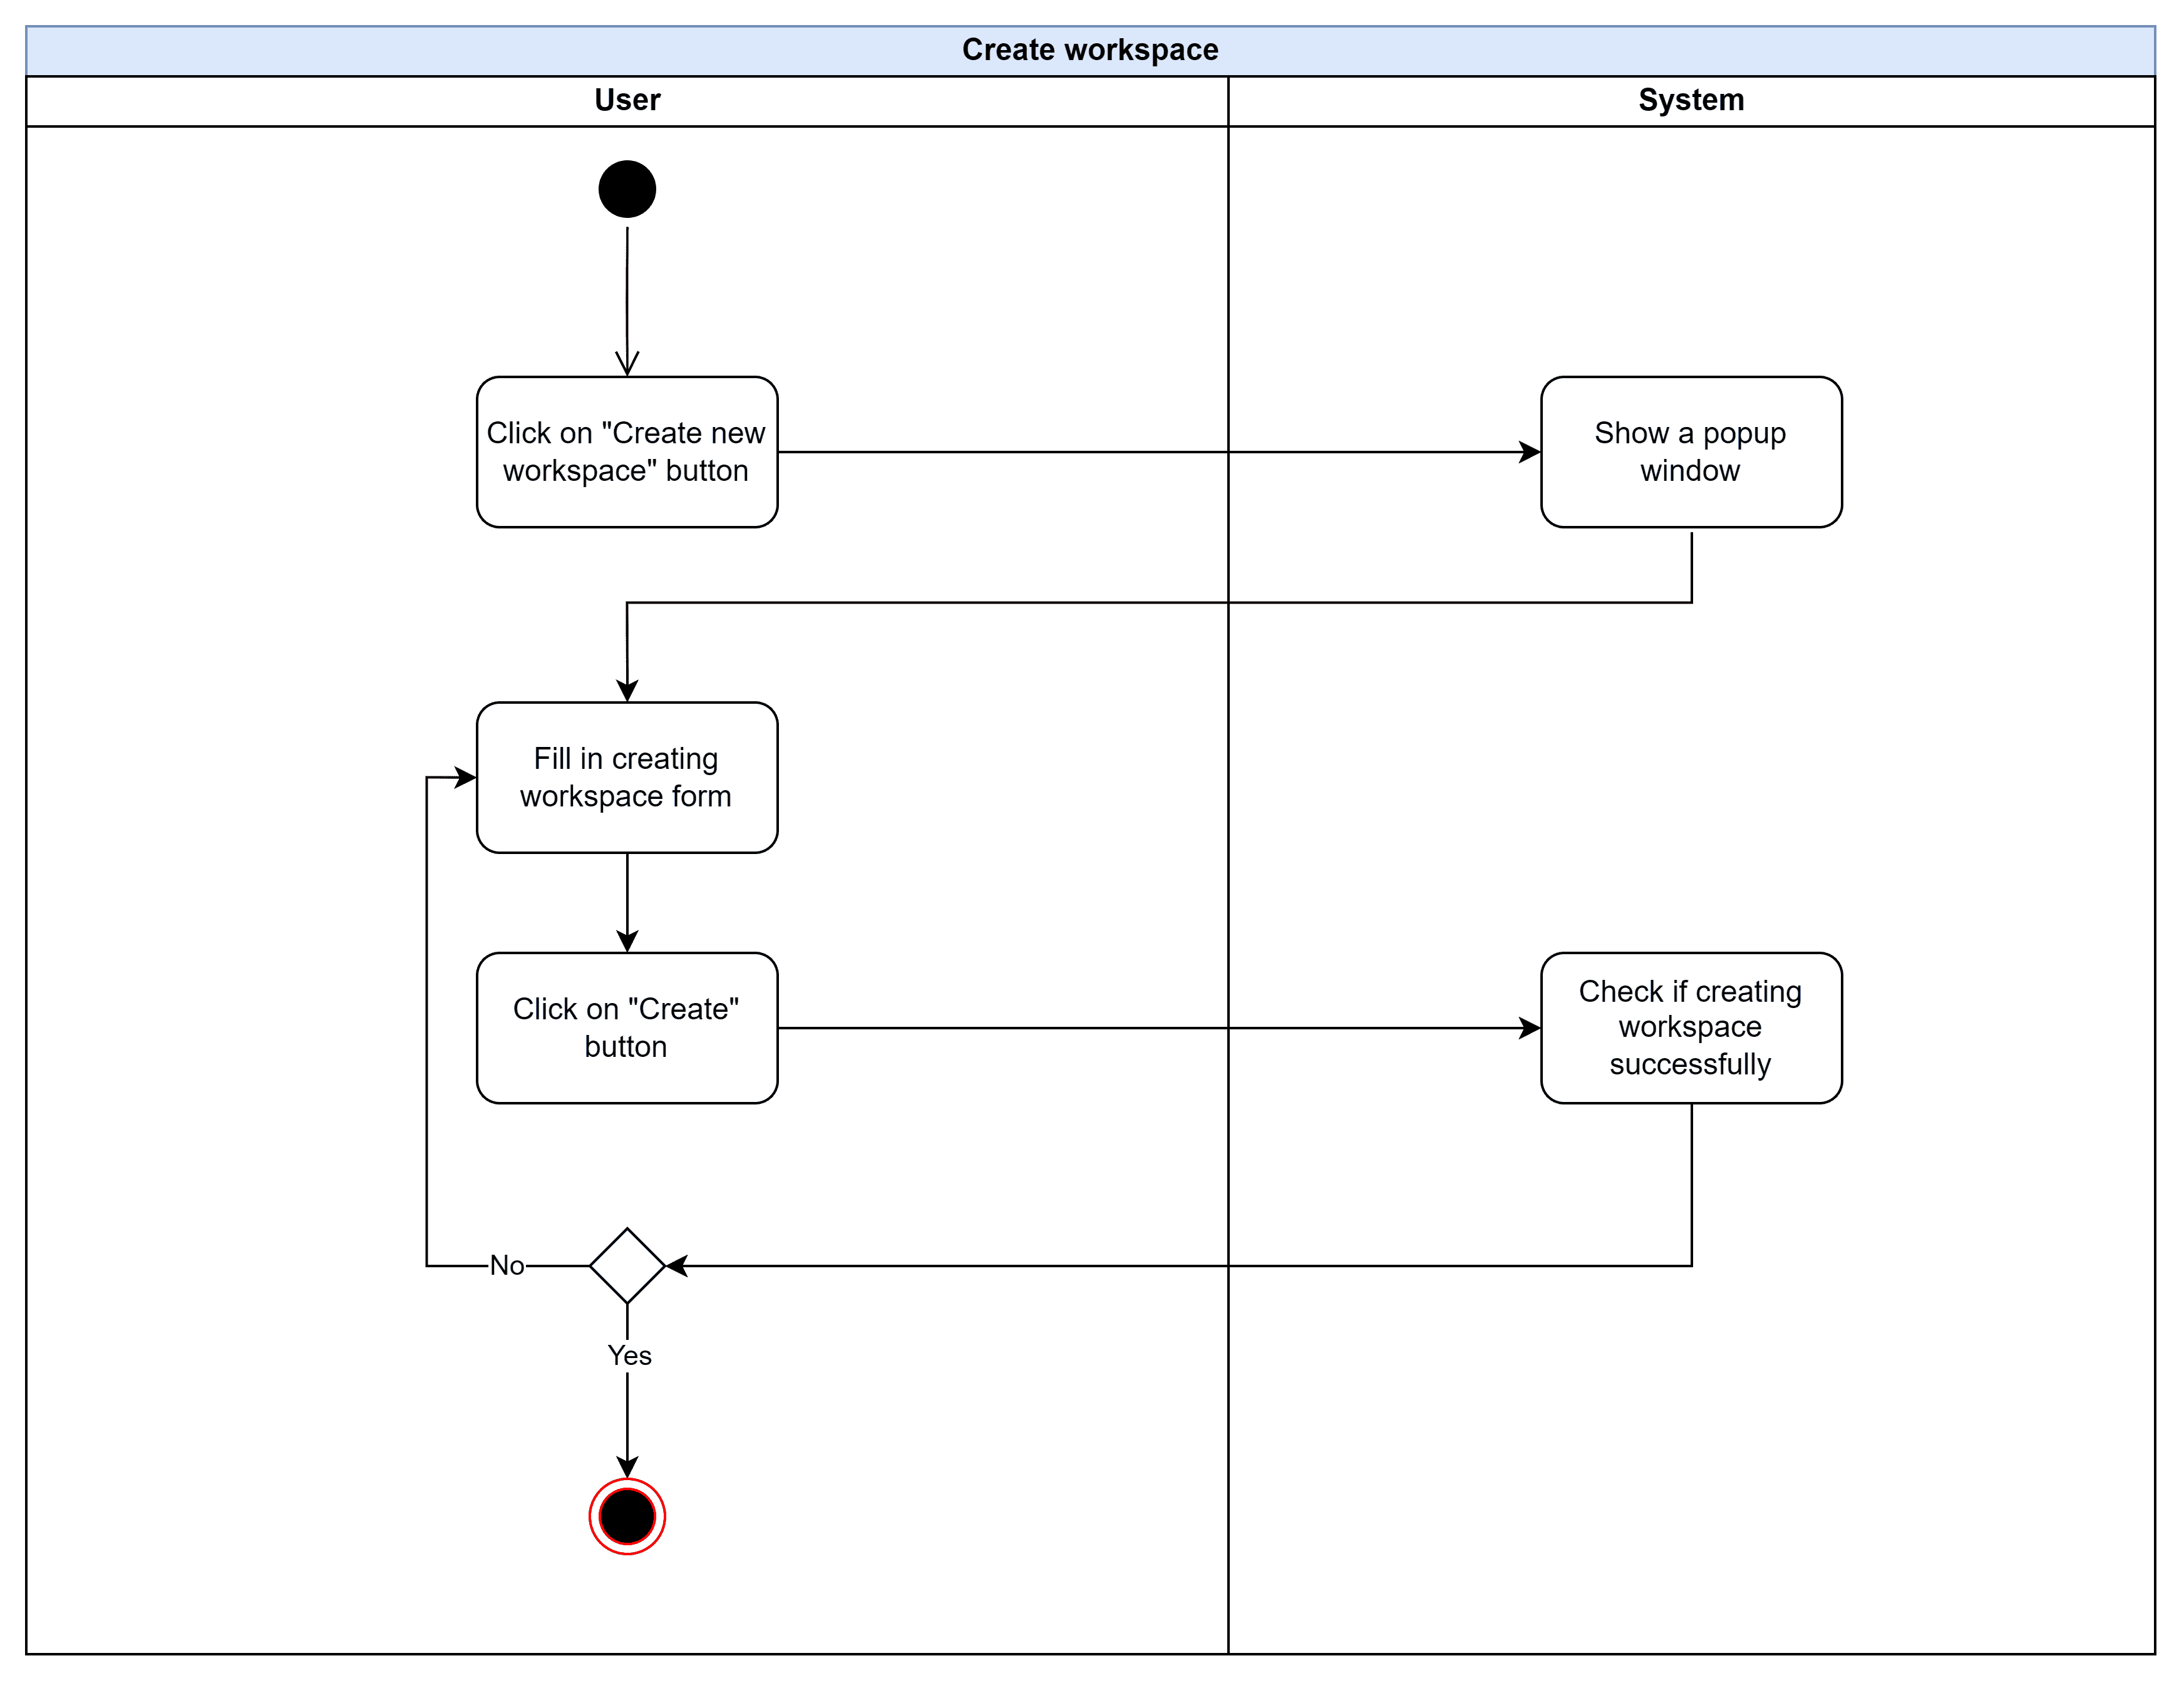
\includegraphics[width=\linewidth]{Content/Phân tích và thiết kế hệ thống/documents/Sơ đồ hoạt động/images/createWorkspace.png}
        \vspace{0.5cm}
        \caption{Tạo mới workspace}
        \label{fig:Tạo mới workspace}
    \end{figure}

\newpage
\subsubsection{Đánh dấu Workspace}
    \begin{figure}[H]
        \centering
        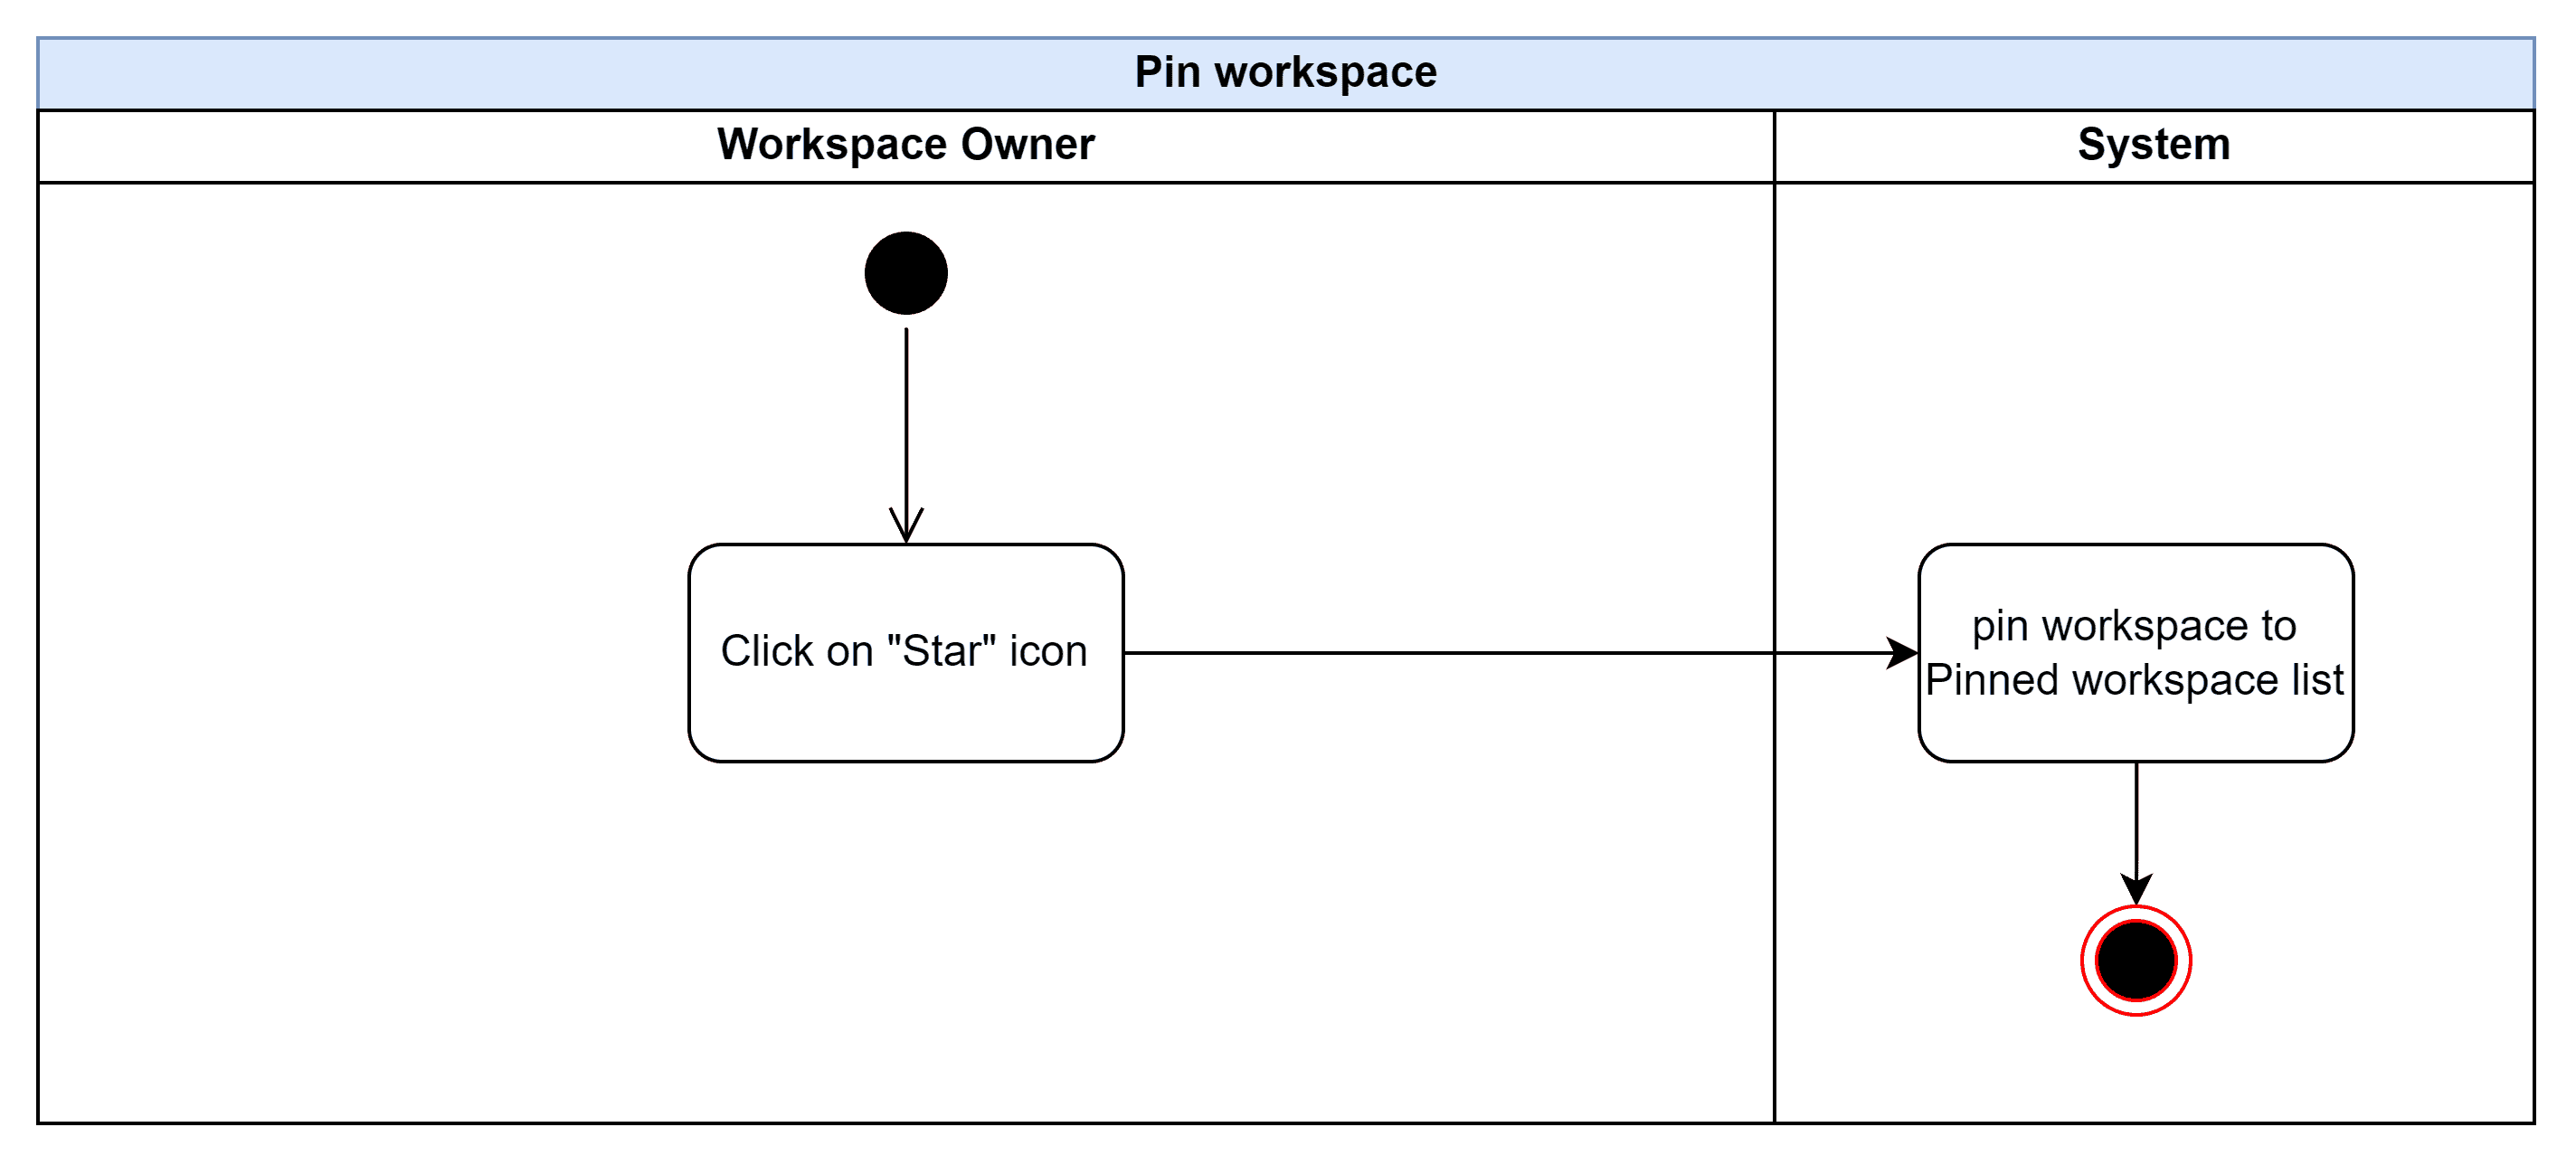
\includegraphics[width=\linewidth]{Content/Phân tích và thiết kế hệ thống/documents/Sơ đồ hoạt động/images/pinWorkspace.png}
        \vspace{0.5cm}
        \caption{Đánh dấu Workspace}
        \label{fig:Đánh dấu Workspace}
    \end{figure}
\newpage
\input{Content/Phân tích và thiết kế hệ thống/documents/Sơ đồ hoạt động/documents/Xoá workspace}

\newpage
\subsubsection{Mở trang quản lý thành viên trong Workspace}
    \begin{figure}[H]
        \centering
        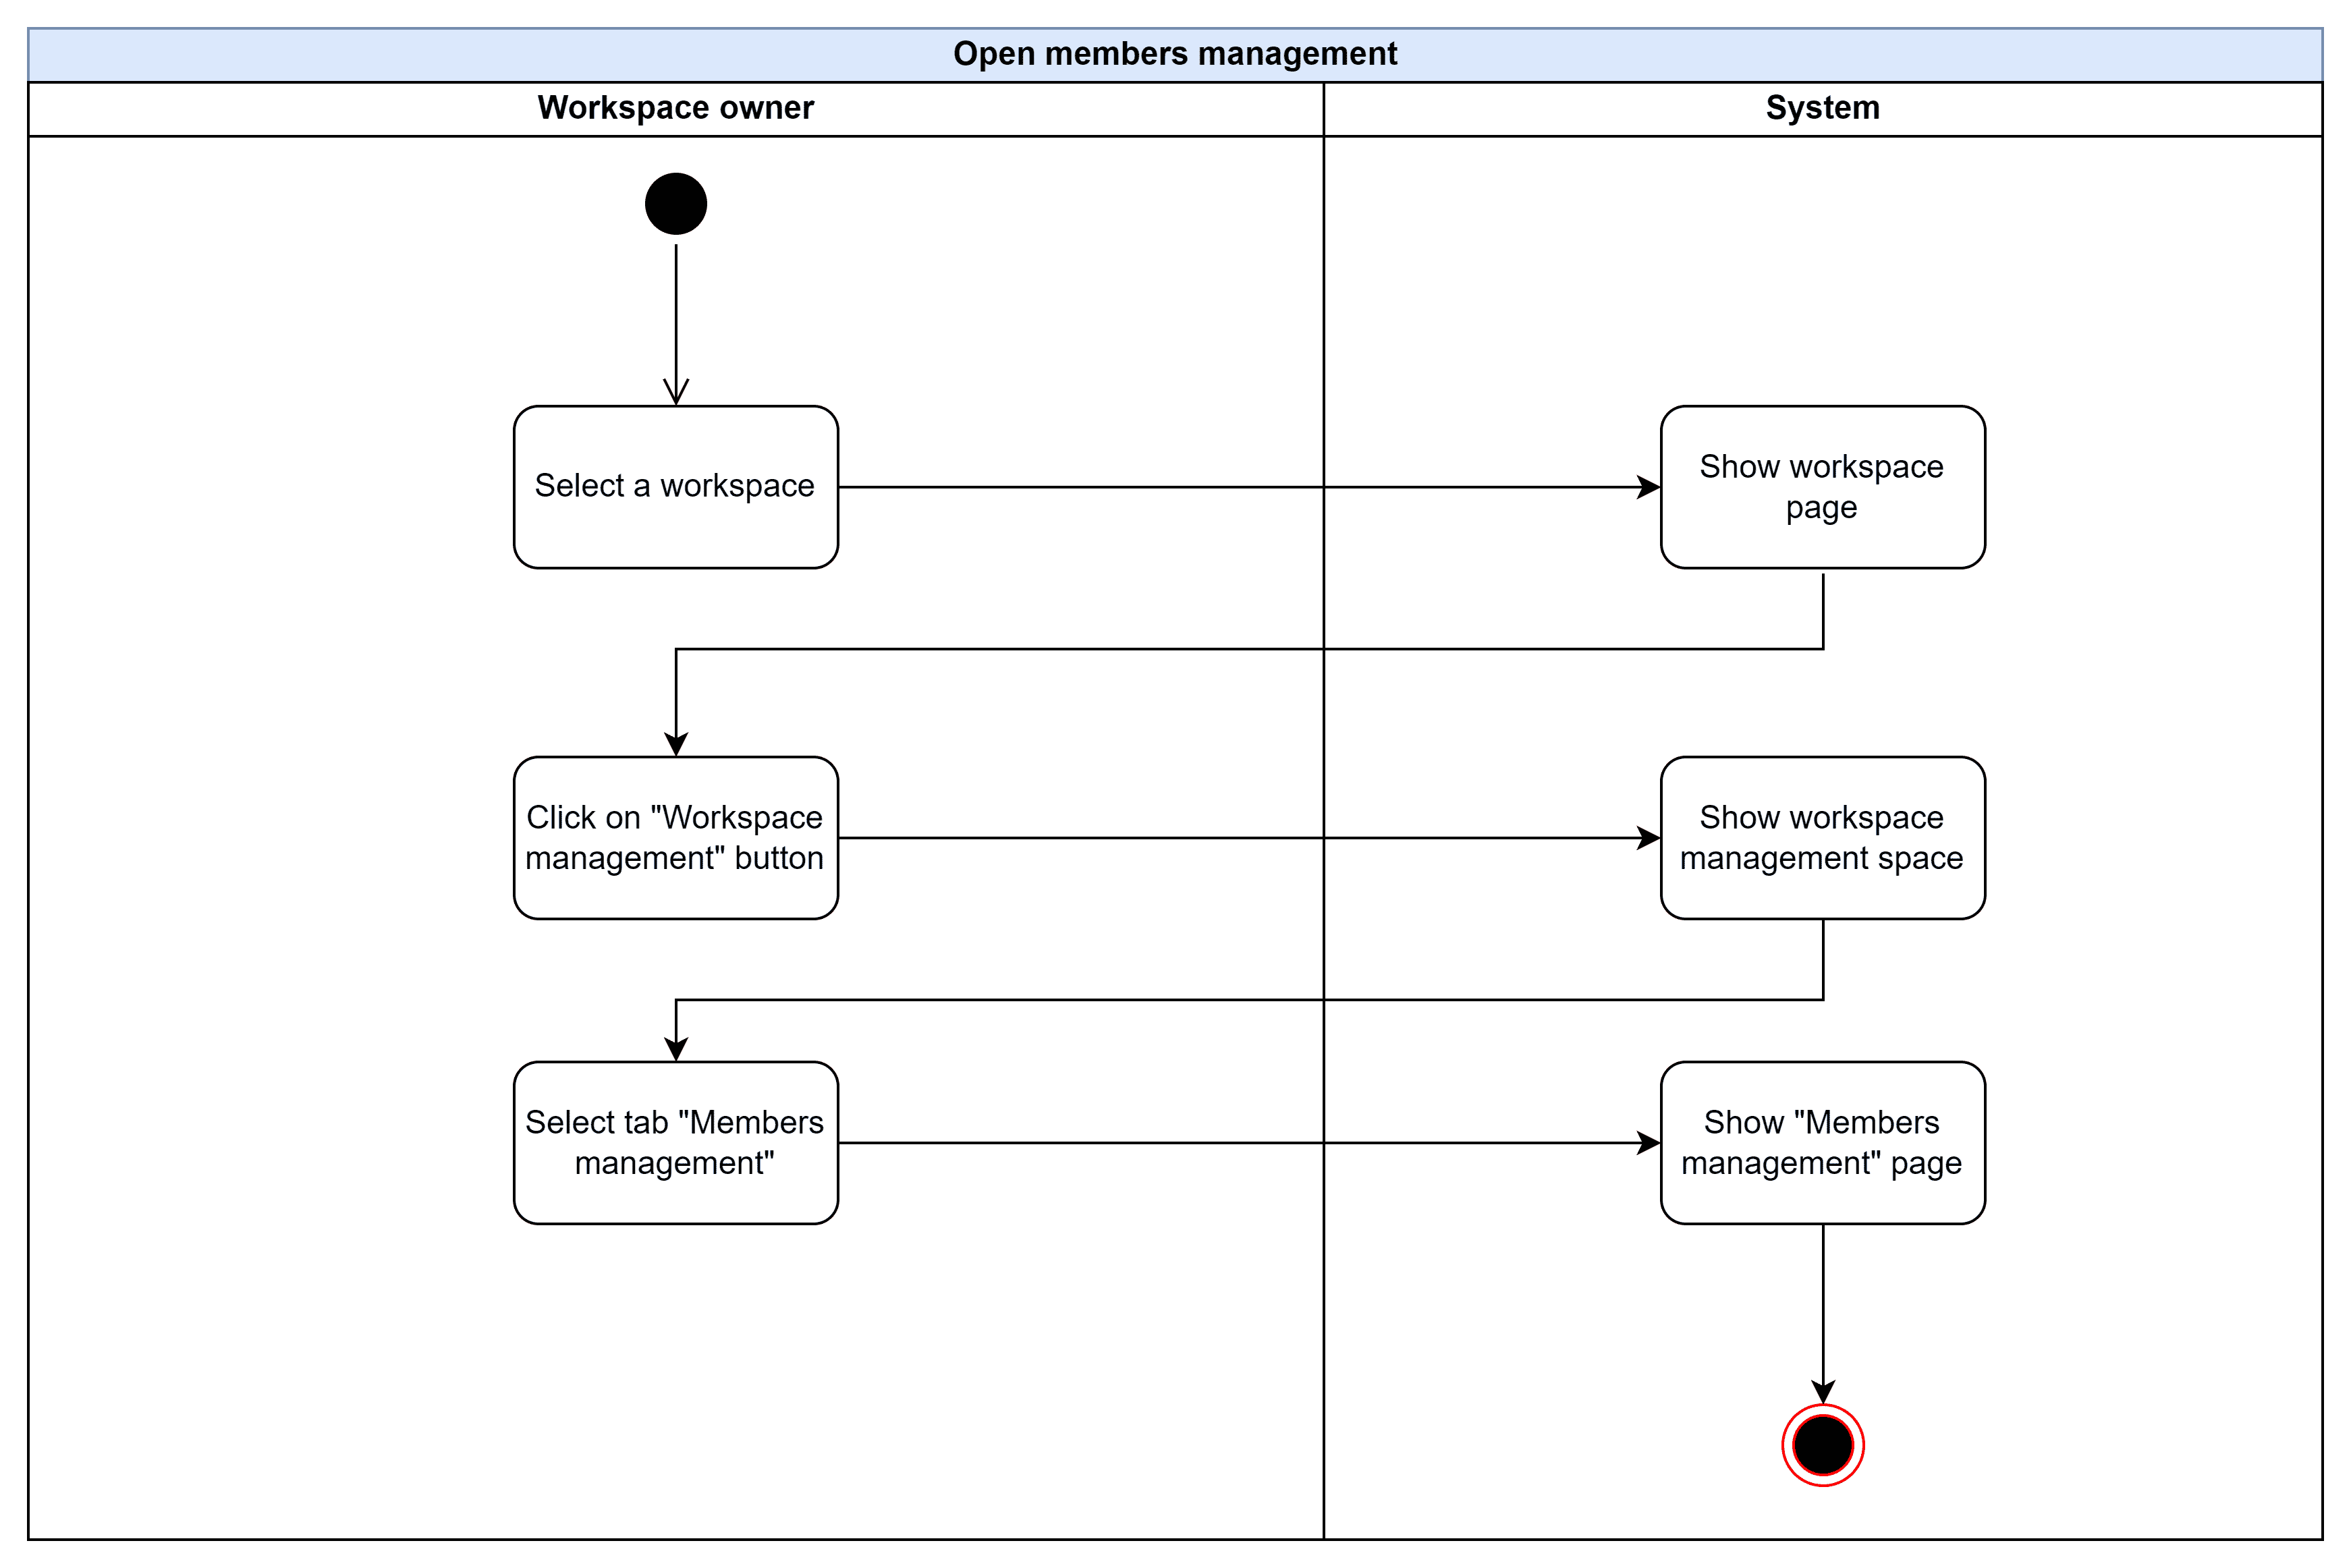
\includegraphics[width=\linewidth]{Content/Phân tích và thiết kế hệ thống/documents/Sơ đồ hoạt động/images/openMemberManagement.png}
        \vspace{0.5cm}
        \caption{Mở trang quản lý thành viên trong Workspace}
        \label{fig:Mở trang quản lý thành viên trong Workspace}
    \end{figure}
\newpage
\subsubsection{Xoá thành viên khỏi Workspace}
    \begin{figure}[H]
        \centering
        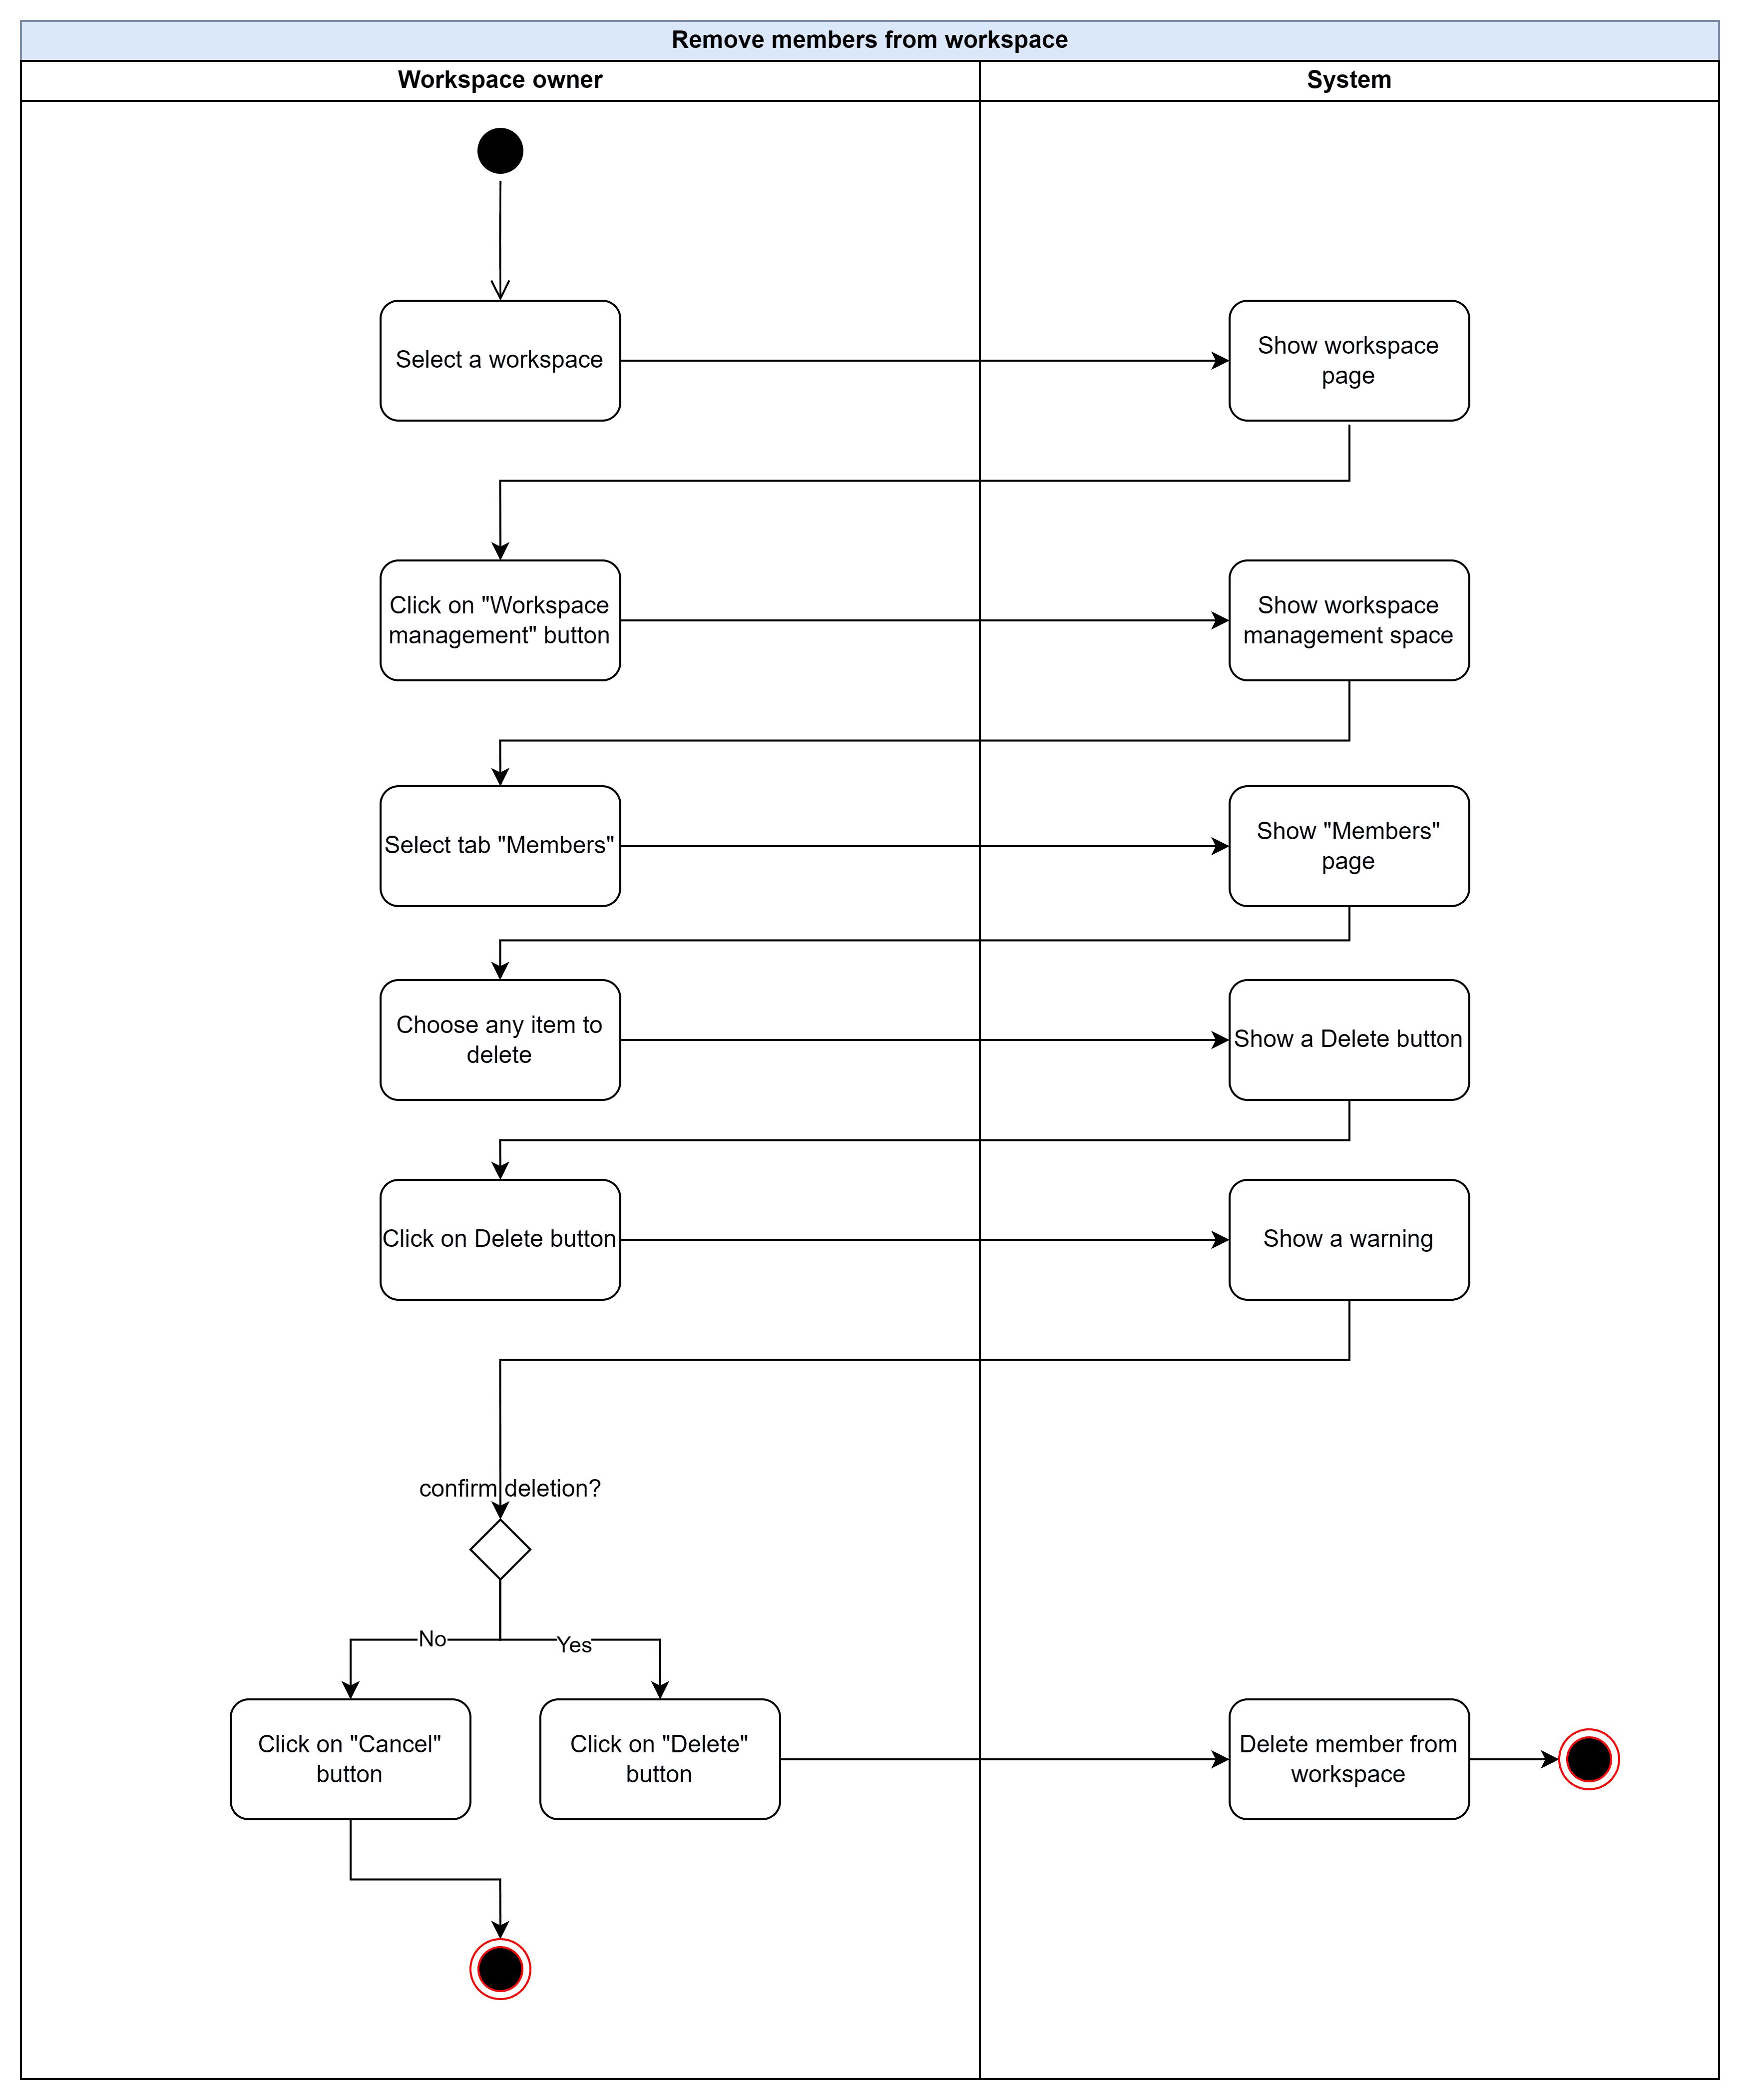
\includegraphics[width=\linewidth]{Content/Phân tích và thiết kế hệ thống/documents/Sơ đồ hoạt động/images/removeMemberFromWorkspace.png}
        \vspace{0.5cm}
        \caption{Xoá thành viên khỏi Workspace}
        \label{fig:Xoá thành viên khỏi Workspace}
    \end{figure}

\newpage
\subsubsection{Mở trang quản lý yêu cầu trong Workspace}
    \begin{figure}[H]
        \centering
        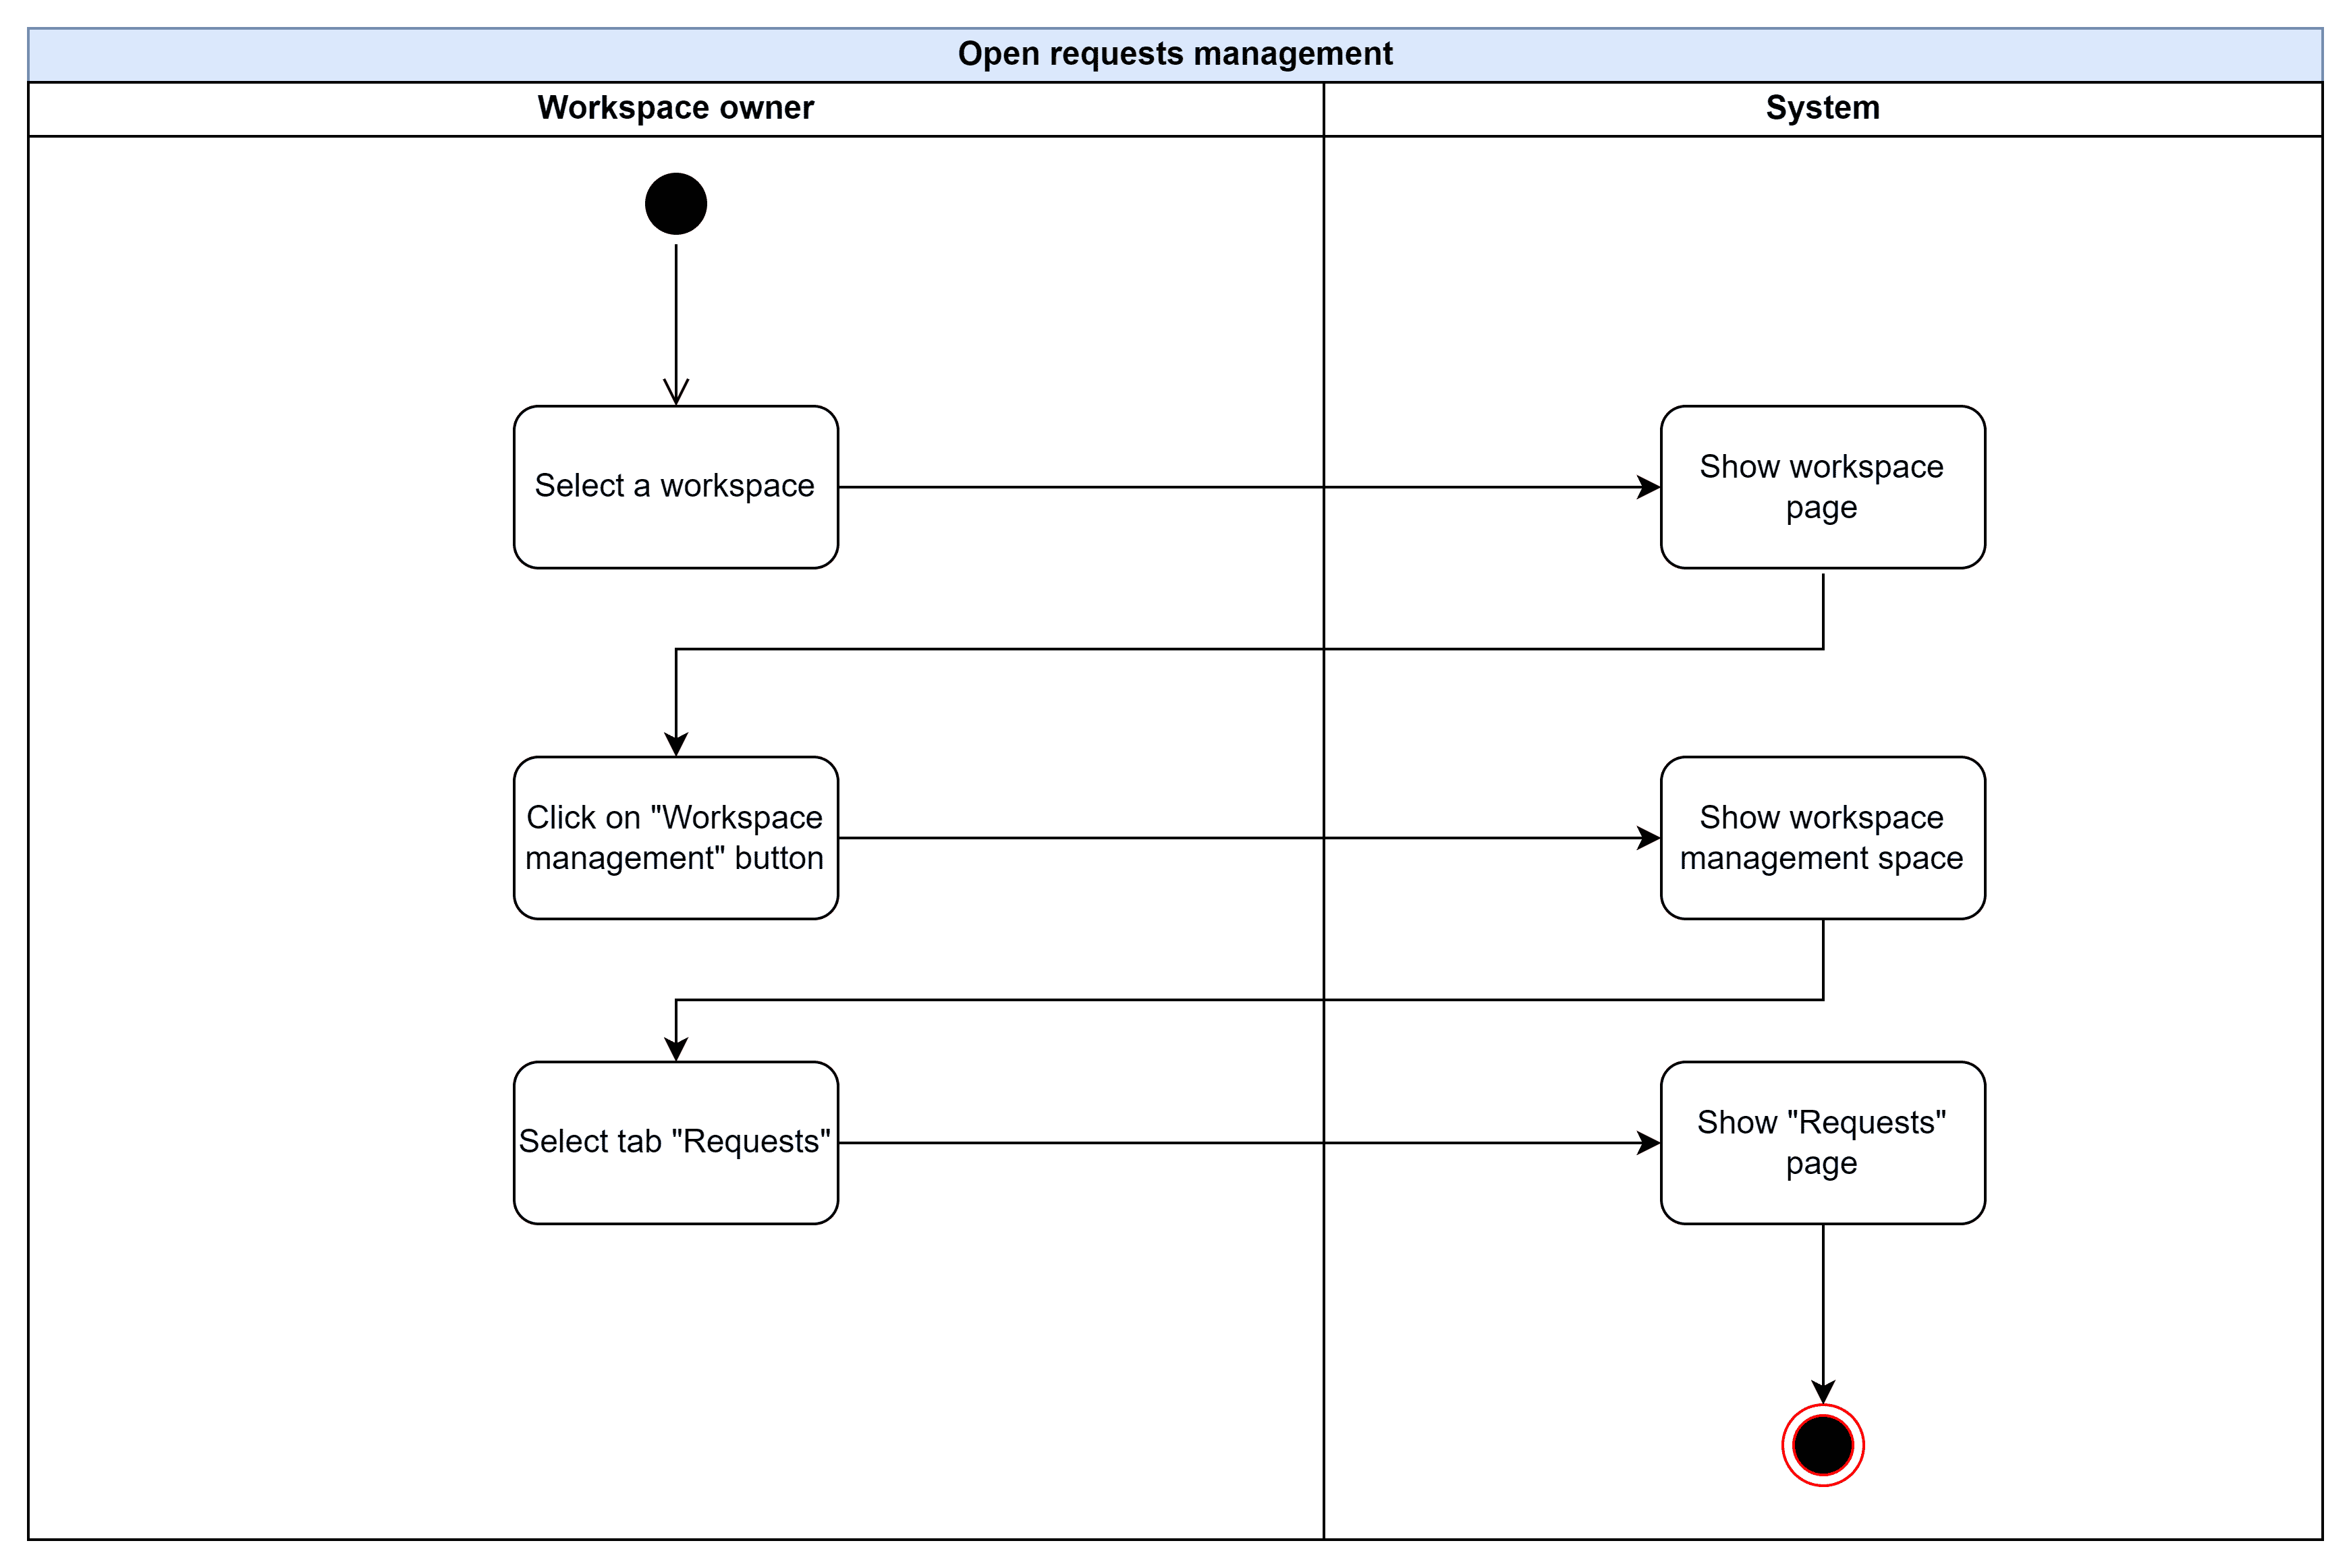
\includegraphics[width=\linewidth]{Content/Phân tích và thiết kế hệ thống/documents/Sơ đồ hoạt động/images/openRequestsManagement.png}
        \vspace{0.5cm}
        \caption{Mở trang quản lý yêu cầu trong Workspace}
        \label{fig:Mở trang quản lý yêu cầu trong Workspace}
    \end{figure}

\newpage
\subsection{Quản lý requests trong Workspace}
    \begin{figure}[H]
        \centering
        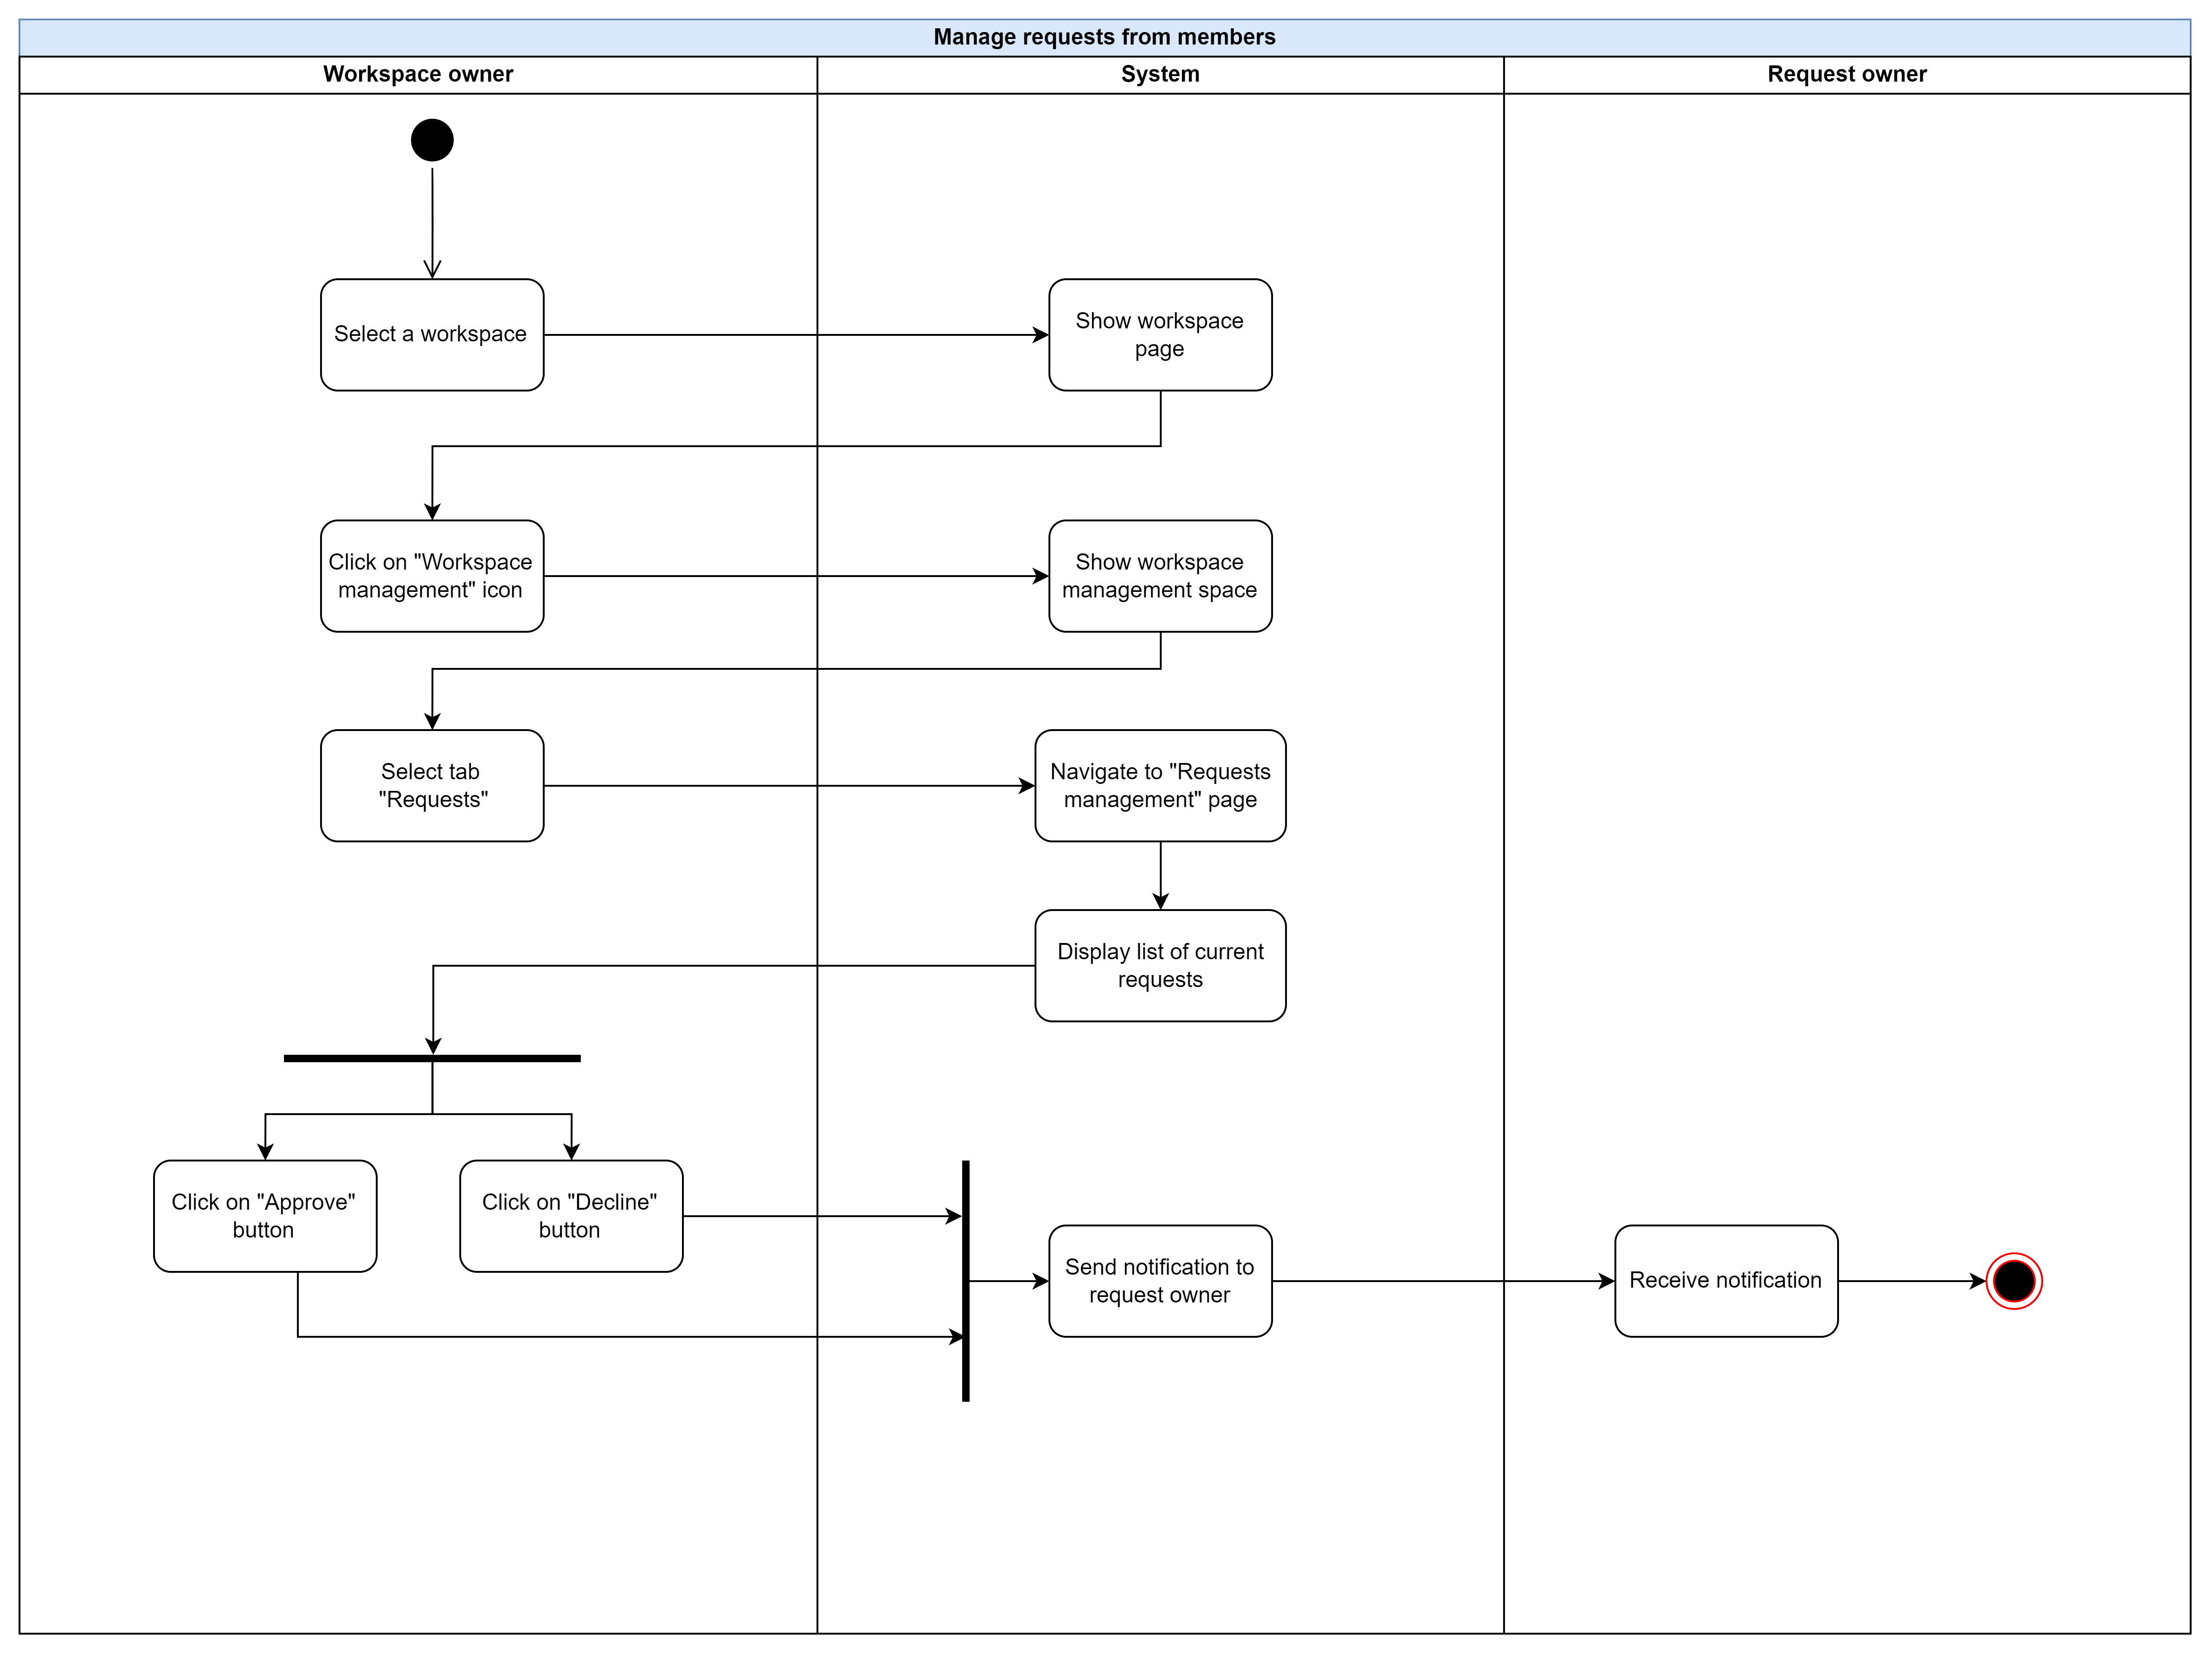
\includegraphics[width=\linewidth]{Content/Phân tích và thiết kế hệ thống/documents/Sơ đồ hoạt động/images/manageRequests.png}
        \vspace{0.5cm}
        \caption{Quản lý requests trong Workspace}
        \label{fig:Quản lý requests trong Workspace}
    \end{figure}

% \newpage
\subsection{Xoá yêu cầu}
    \begin{figure}[H]
        \centering
        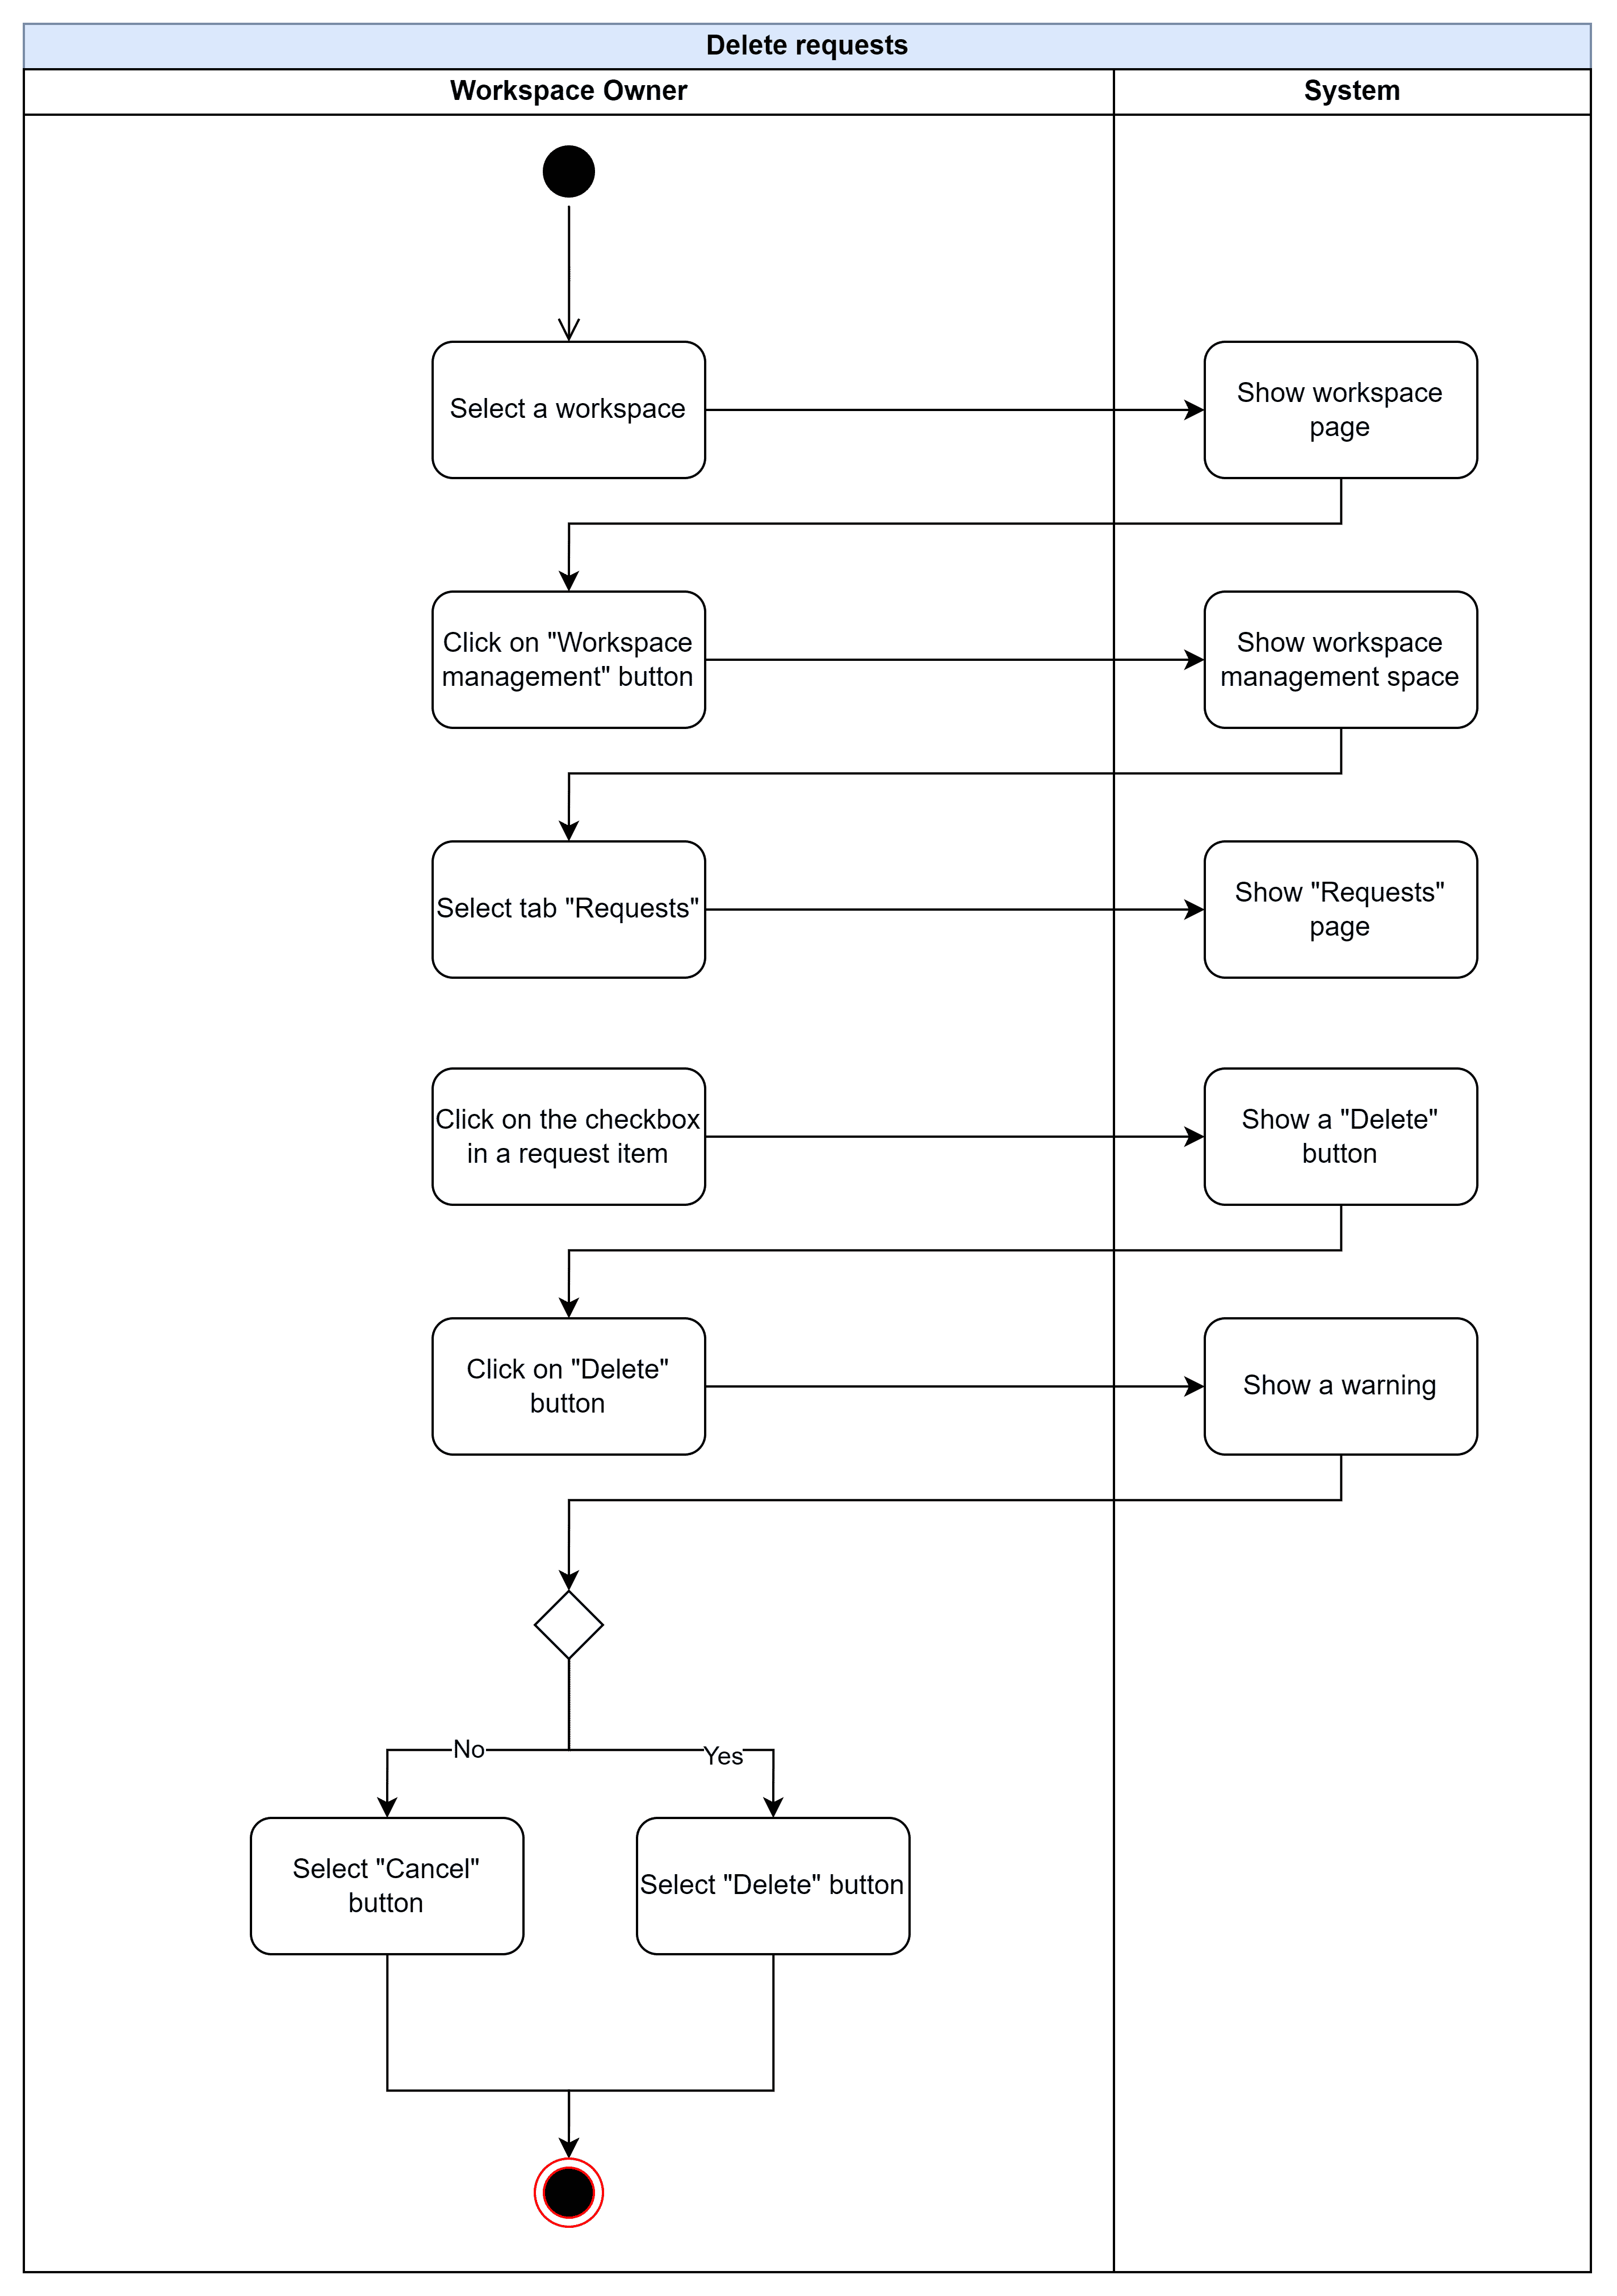
\includegraphics[width=0.8\linewidth]{Content/Phân tích và thiết kế hệ thống/documents/Sơ đồ hoạt động/images/deleteRequests.png}
        \vspace{0.5cm}
        \caption{Xoá yêu cầu}
        \label{fig:Xoá yêu cầu}
    \end{figure}

\newpage
\subsection{Thay đổi quyền của thành viên trong Workspace}
    \begin{figure}[H]
        \centering
        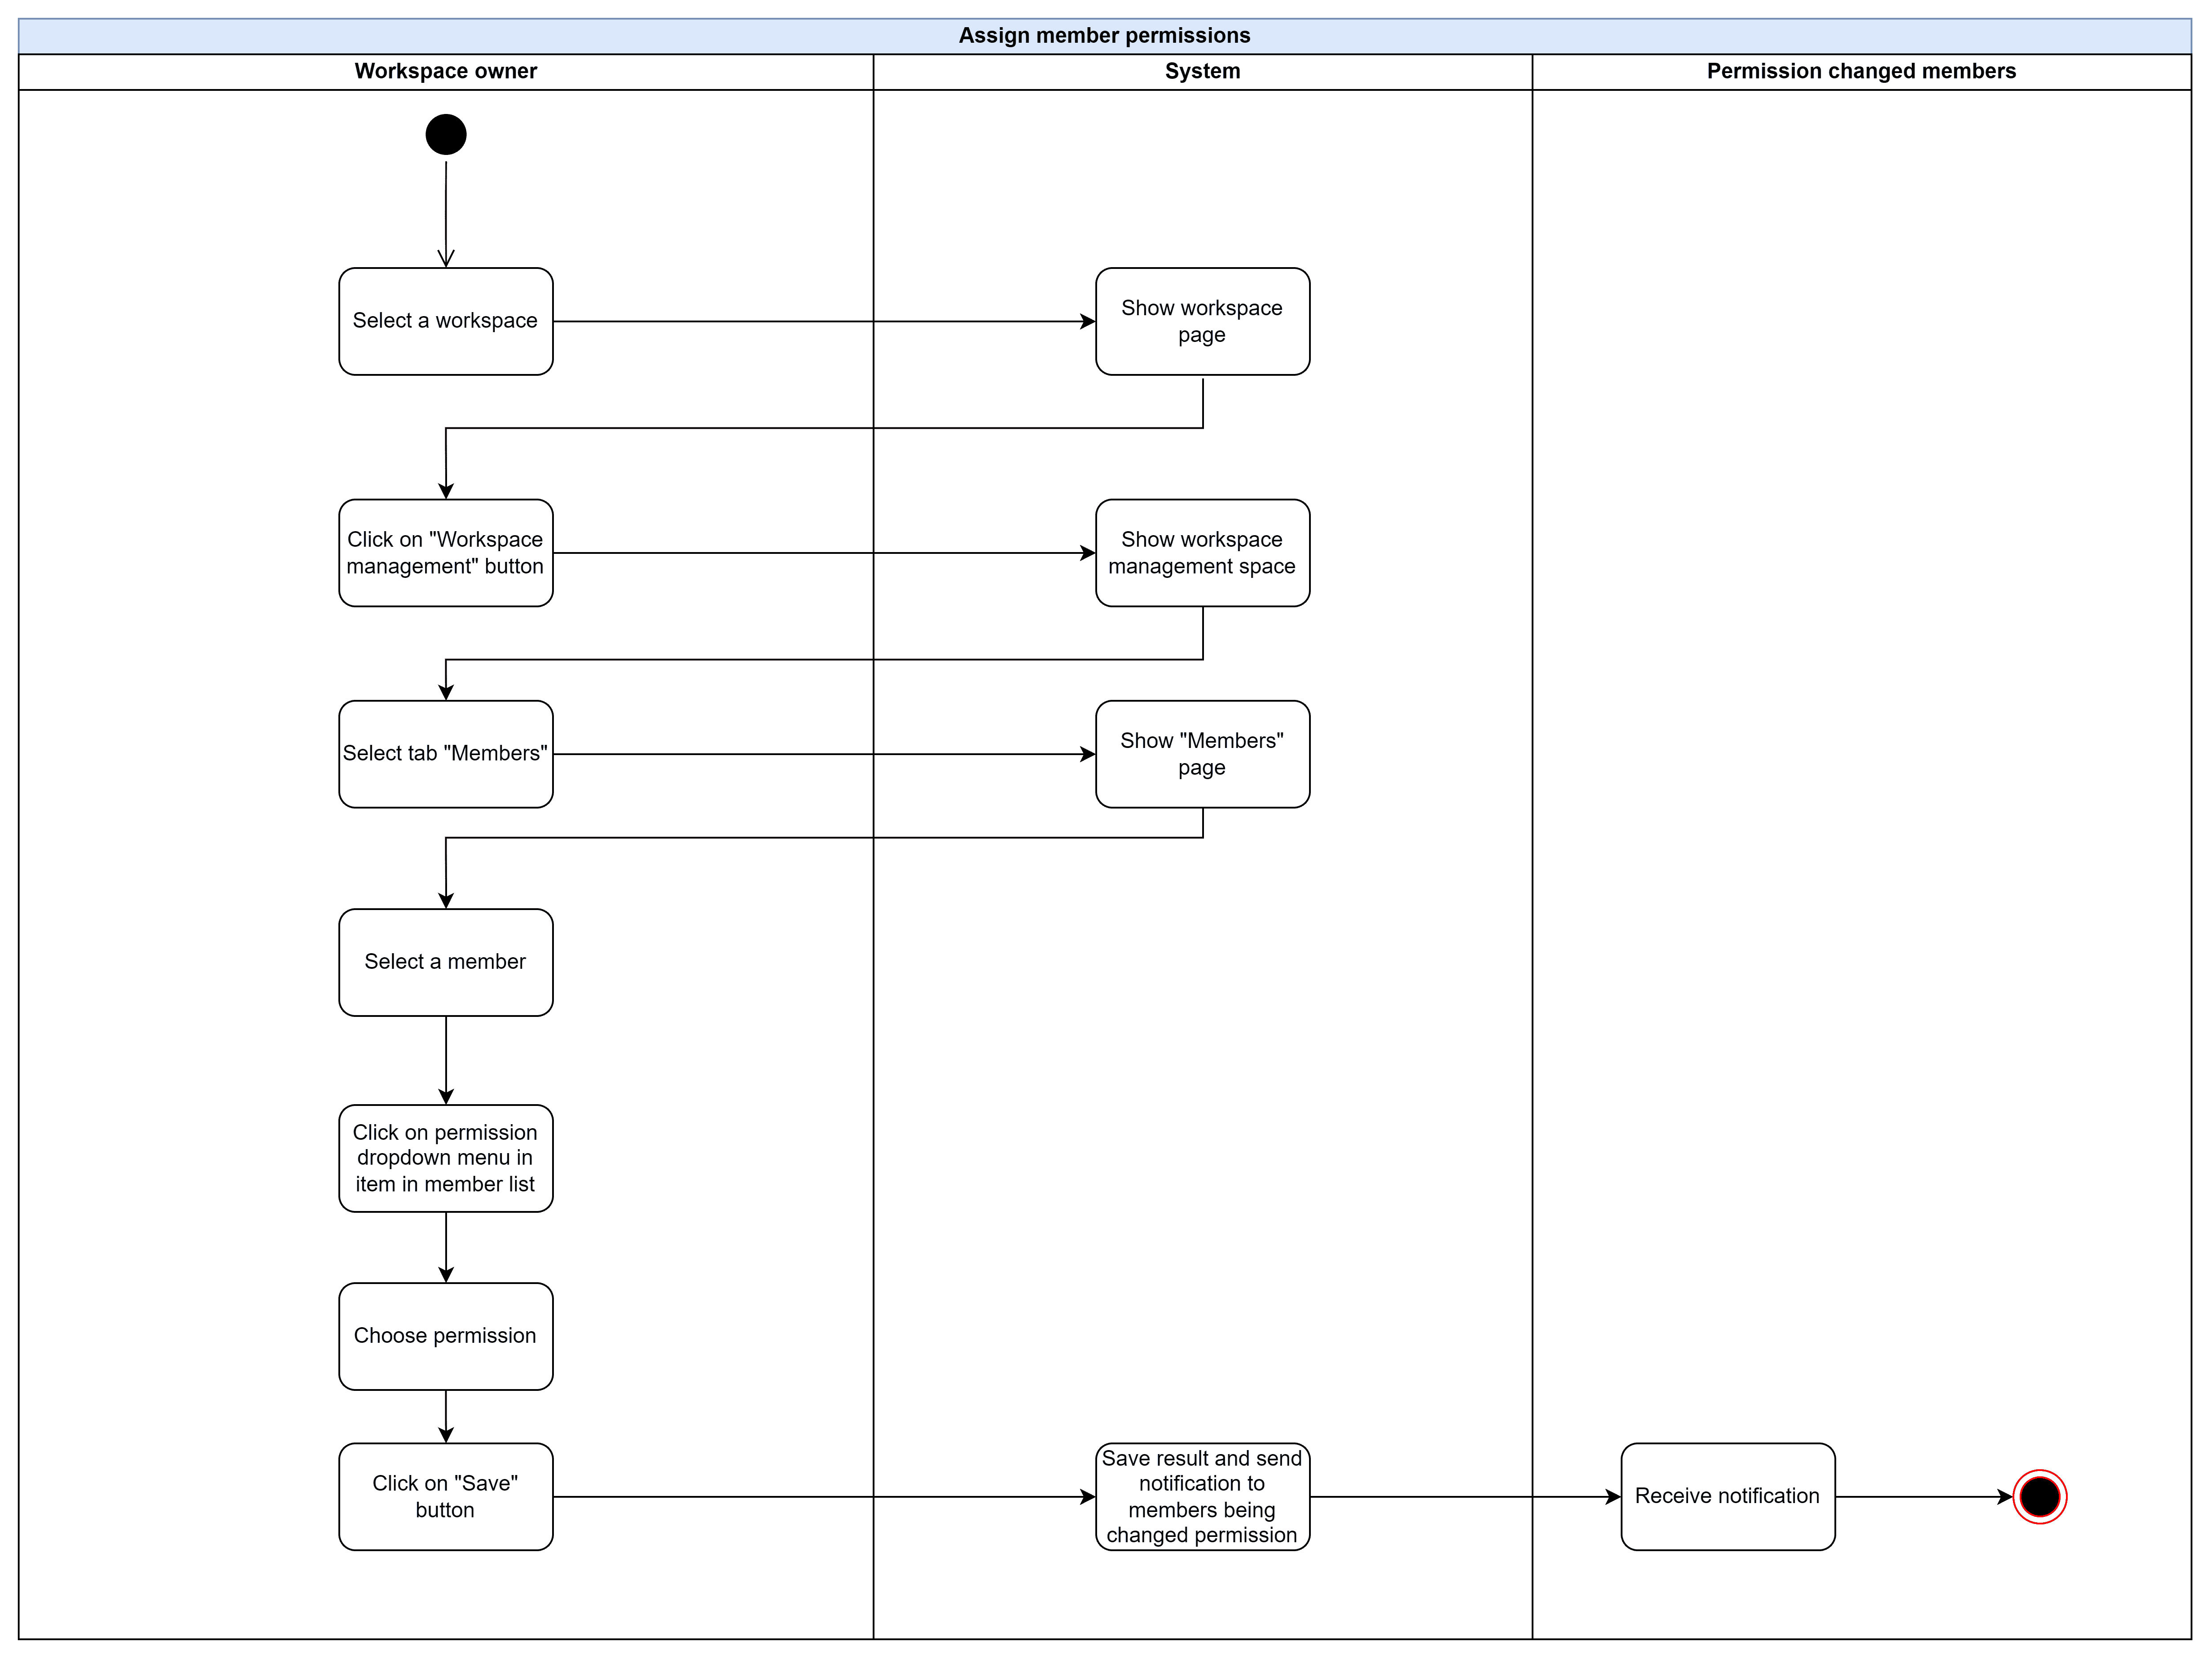
\includegraphics[width=\linewidth]{Content/Phân tích và thiết kế hệ thống/documents/Sơ đồ hoạt động/images/adjustMemberPermissions.png}
        \vspace{0.5cm}
        \caption{Thay đổi quyền của thành viên trong Workspace}
        \label{fig:Thay đổi quyền của thành viên trong Workspace}
    \end{figure}

\newpage
\subsection{Xem danh sách dự án trong Workspace}
    \begin{figure}[H]
        \centering
        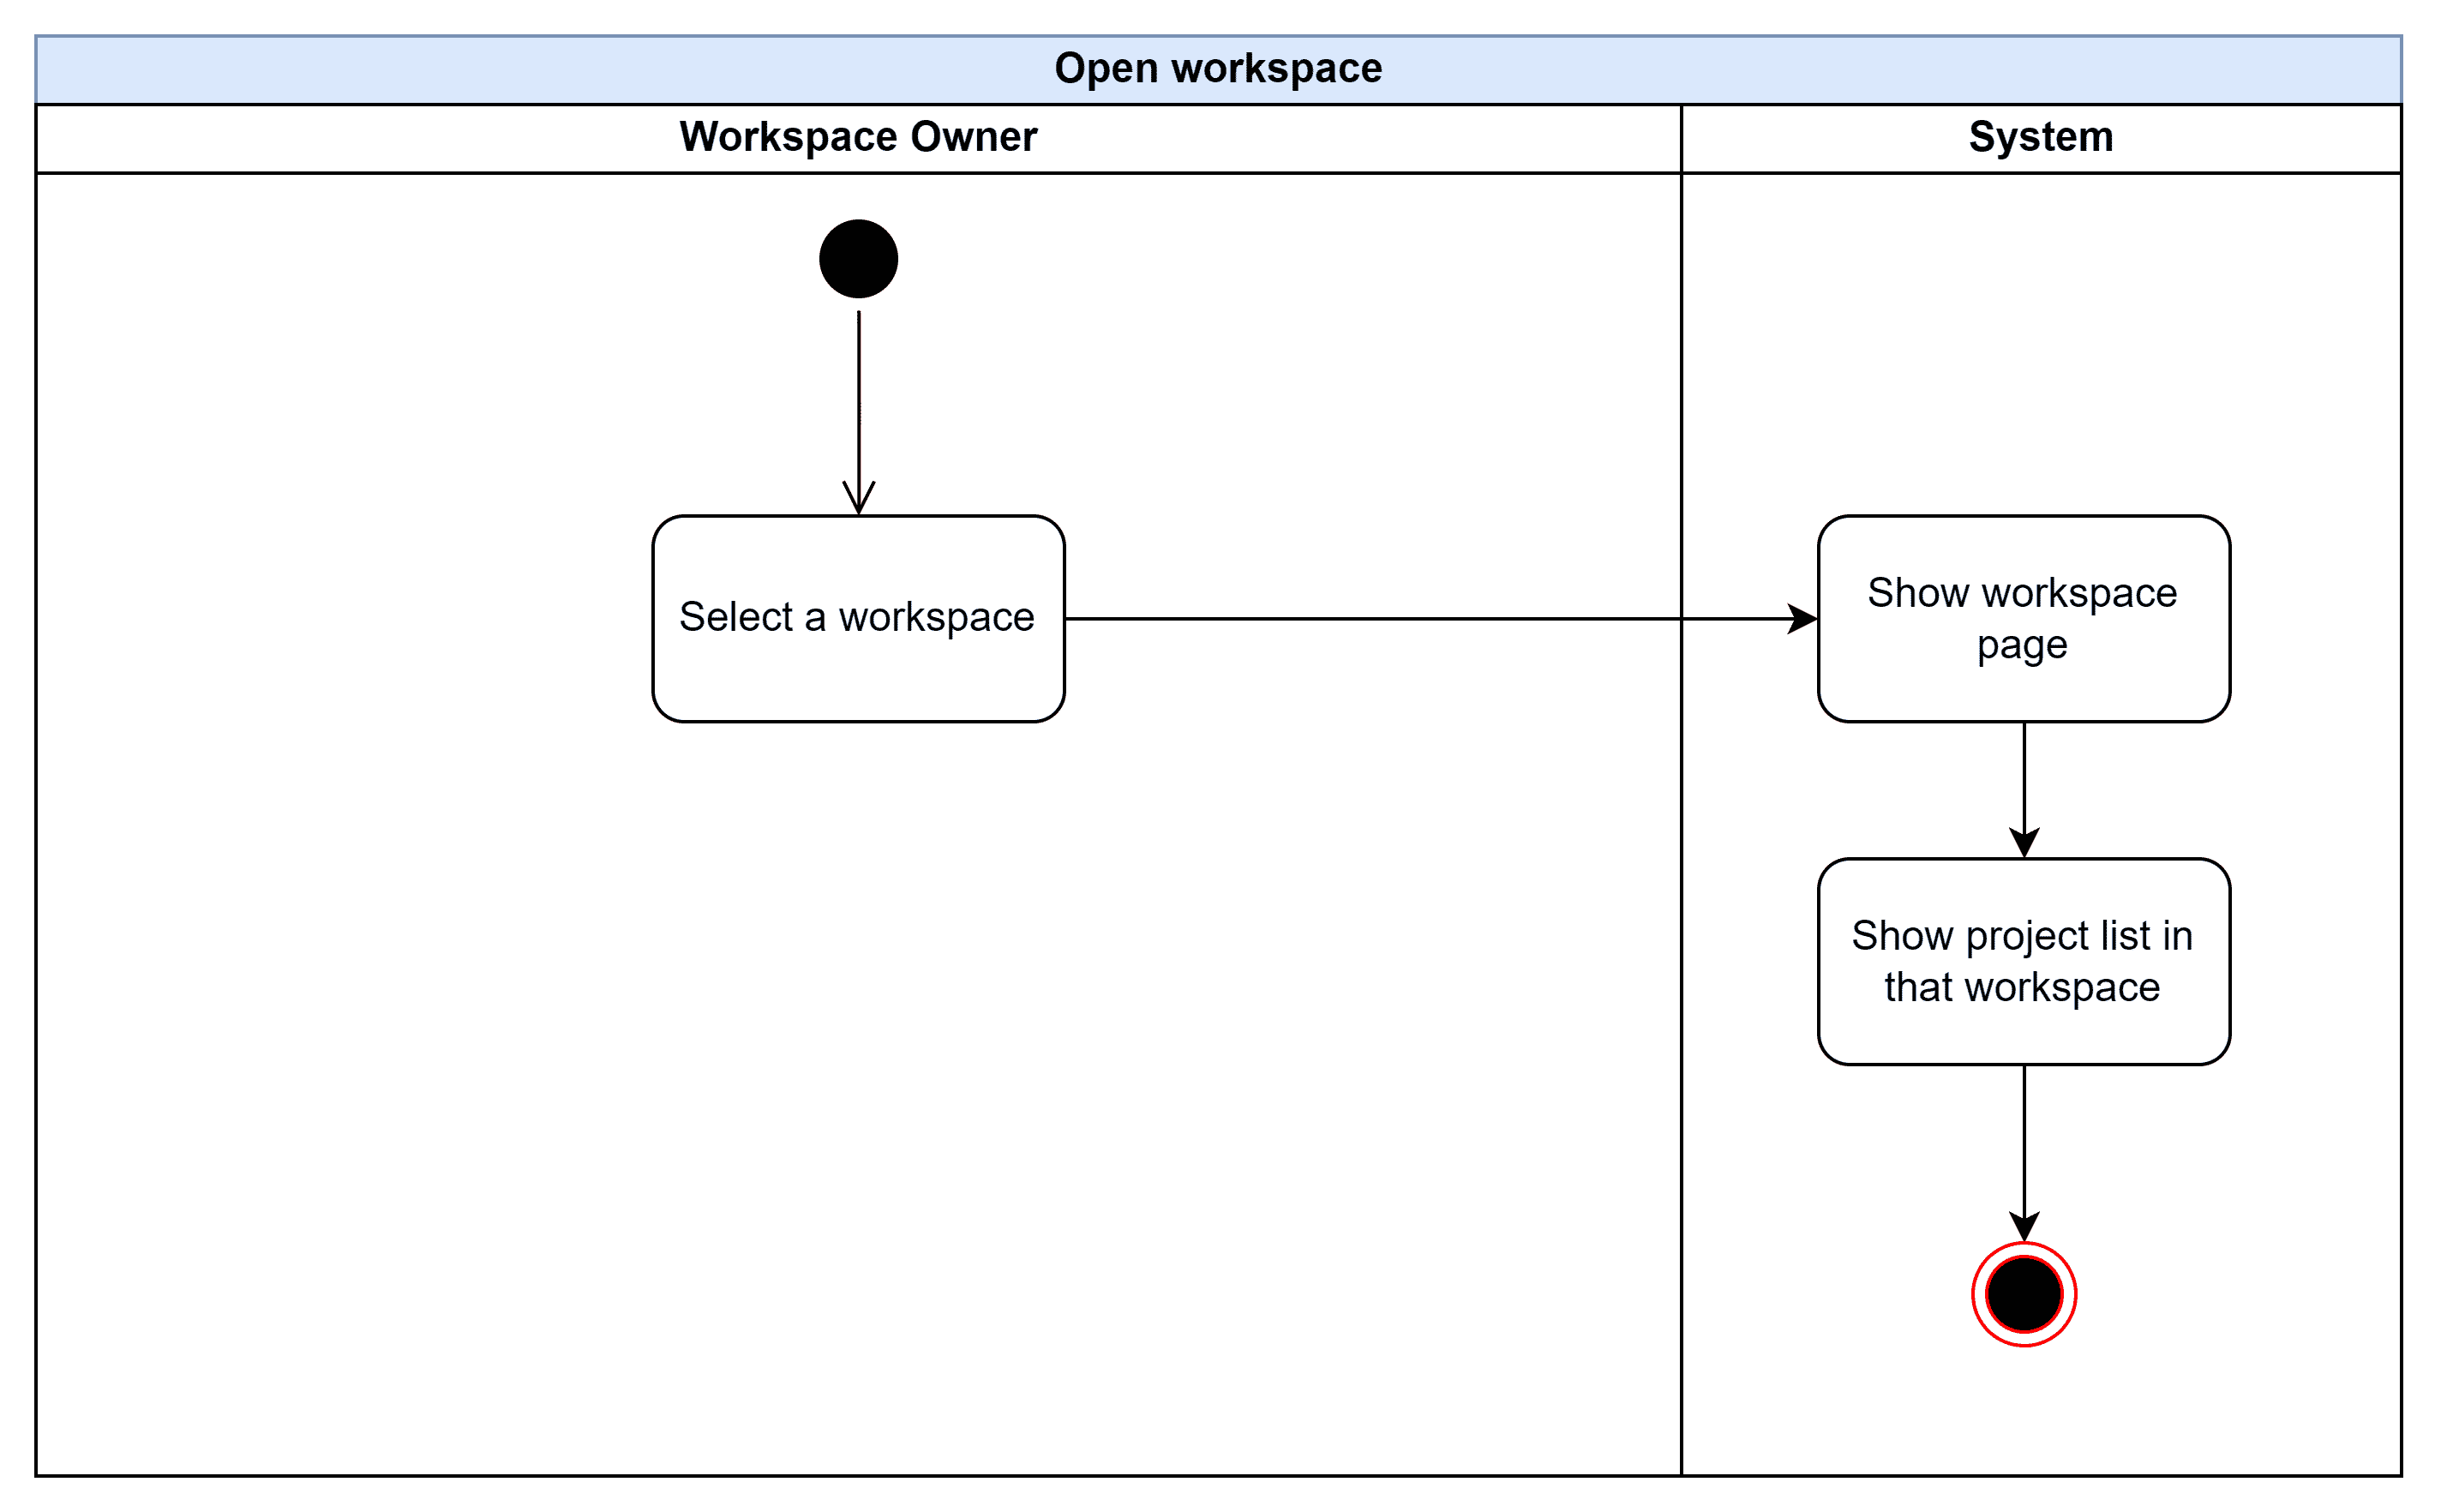
\includegraphics[width=\linewidth]{Content/Phân tích và thiết kế hệ thống/documents/Sơ đồ hoạt động/images/openWorkspace.png}
        \vspace{0.5cm}
        \caption{Xem danh sách dự án trong Workspace}
        \label{fig:Xem danh sách dự án trong Workspace}
    \end{figure}

\newpage
\subsubsection{Tạo mới project trong Workspace}
    \begin{figure}[H]
        \centering
        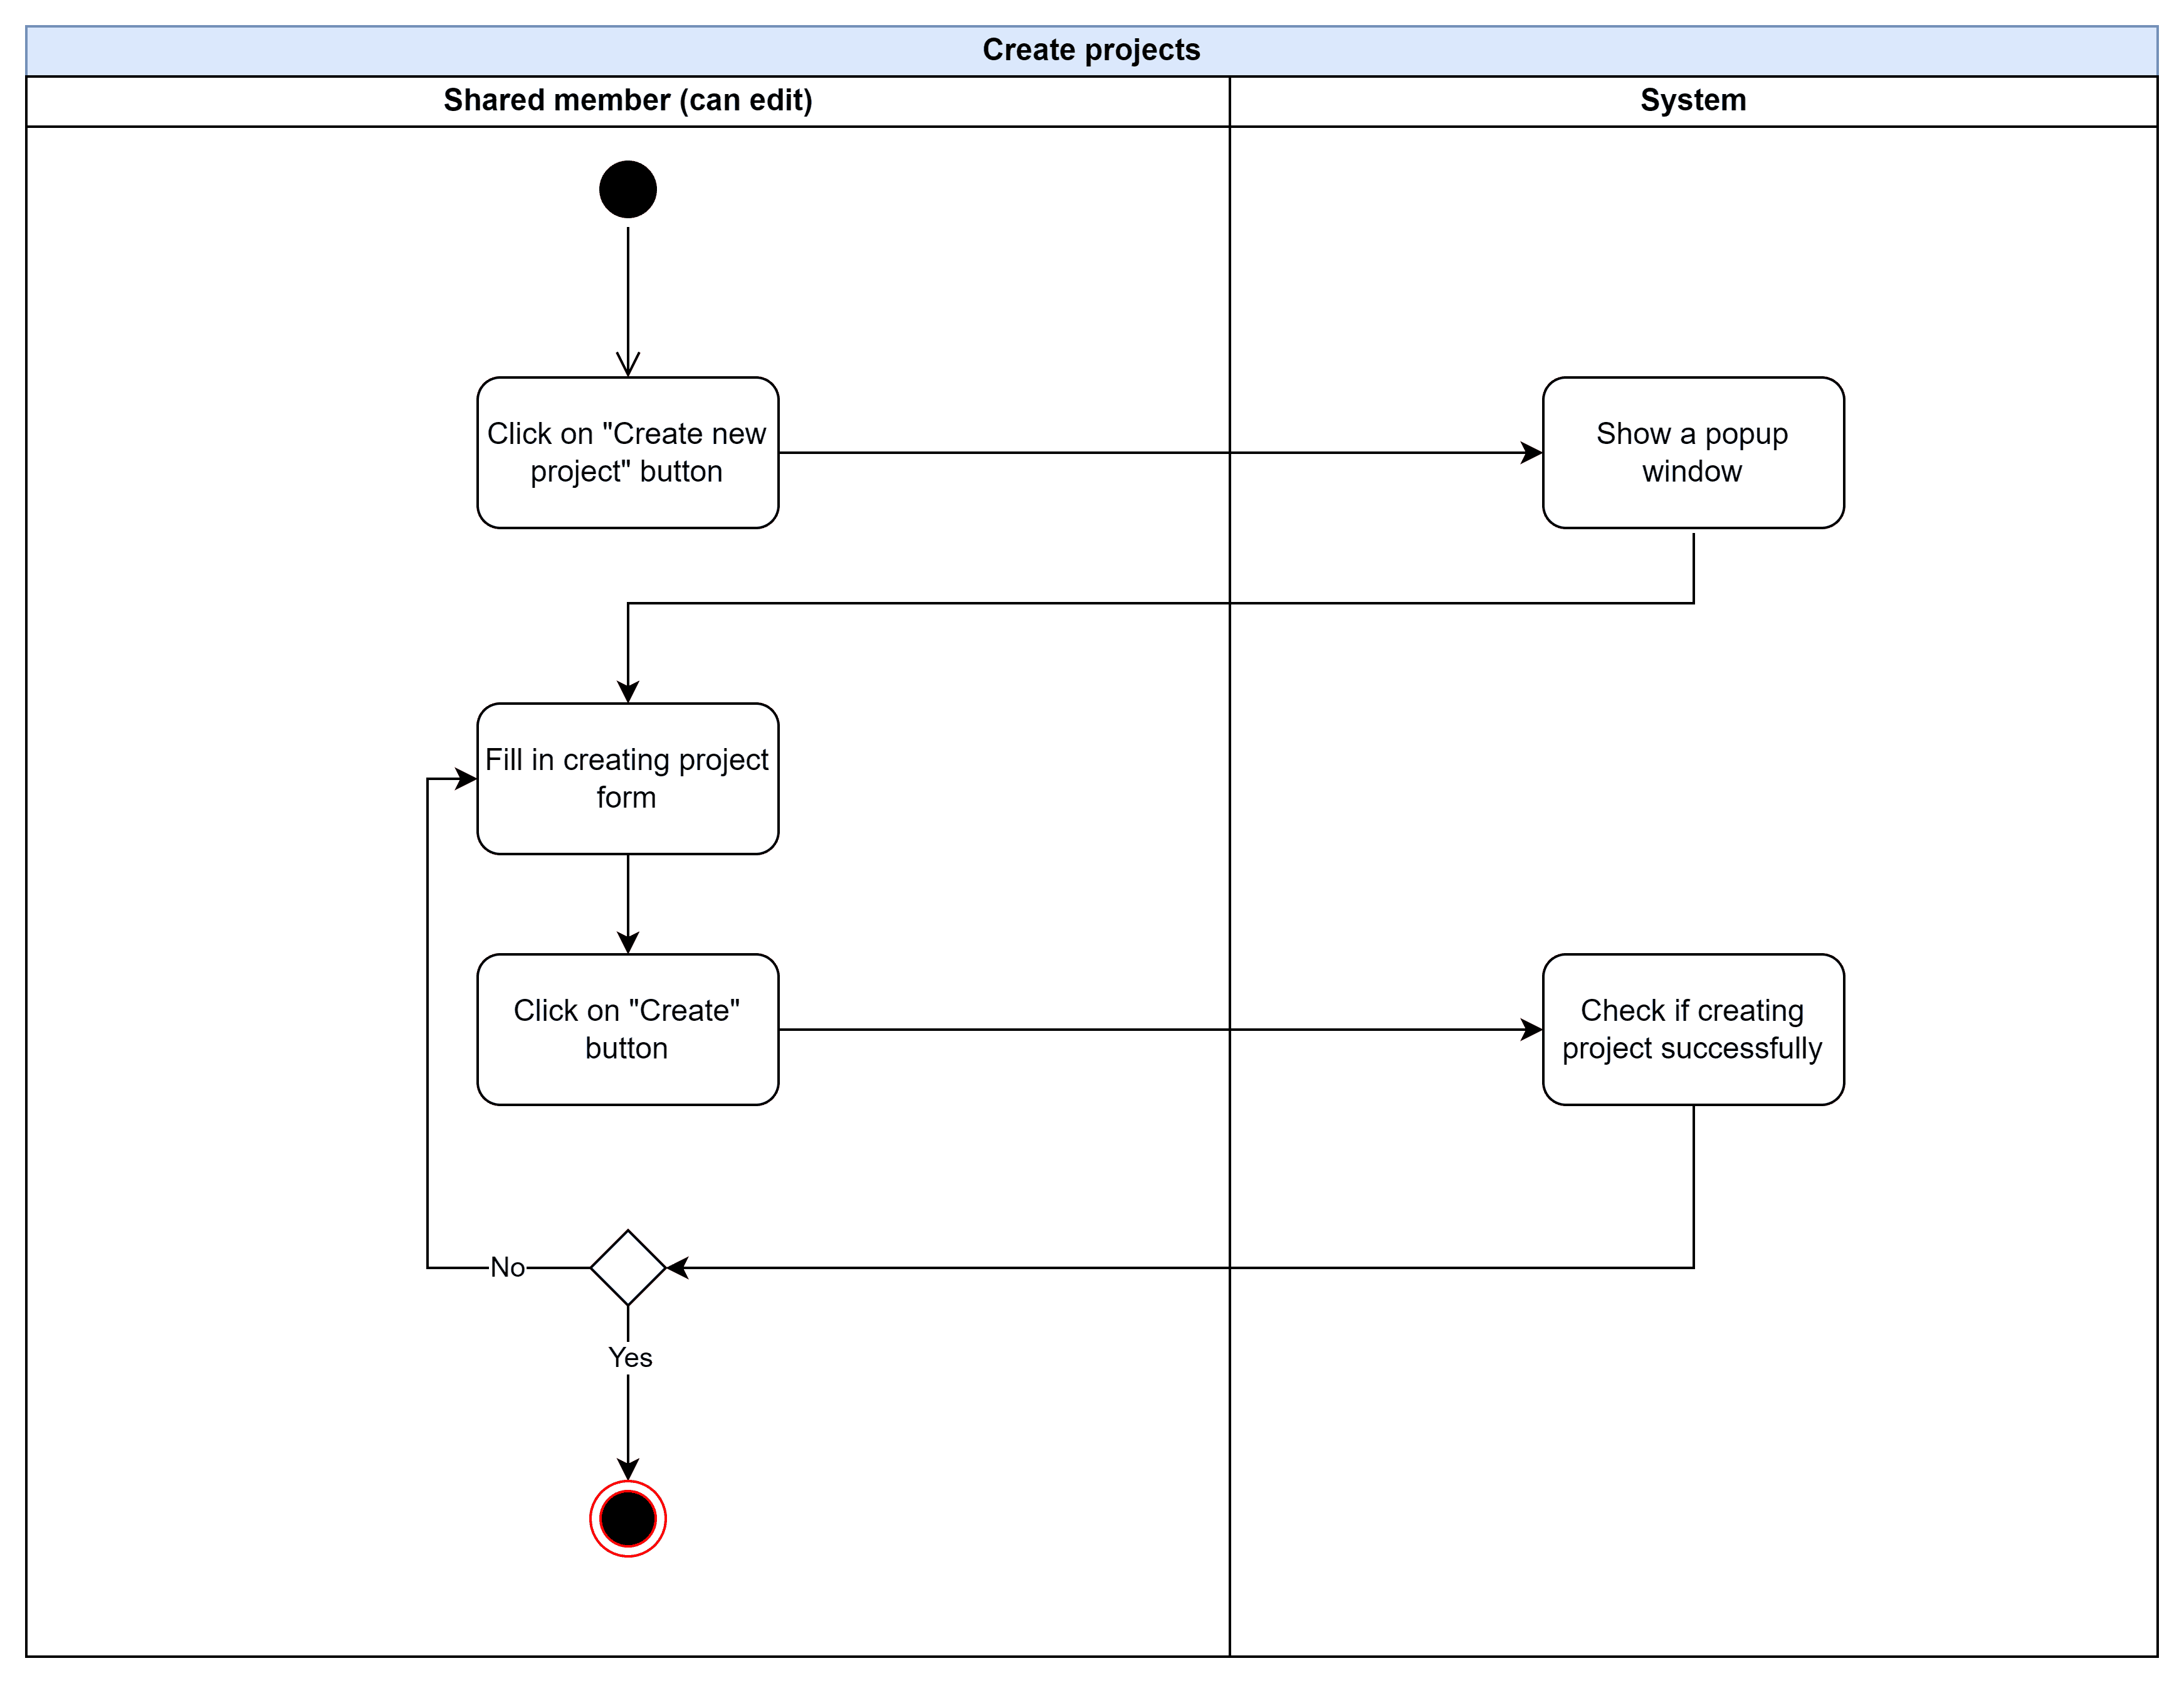
\includegraphics[width=\linewidth]{Content/Phân tích và thiết kế hệ thống/documents/Sơ đồ hoạt động/images/createProjects.png}
        \vspace{0.5cm}
        \caption{Tạo mới project trong Workspace}
        \label{fig:Tạo mới project trong Workspace}
    \end{figure}

\newpage
\subsection{Xoá project trong Workspace}
    \begin{figure}[H]
        \centering
        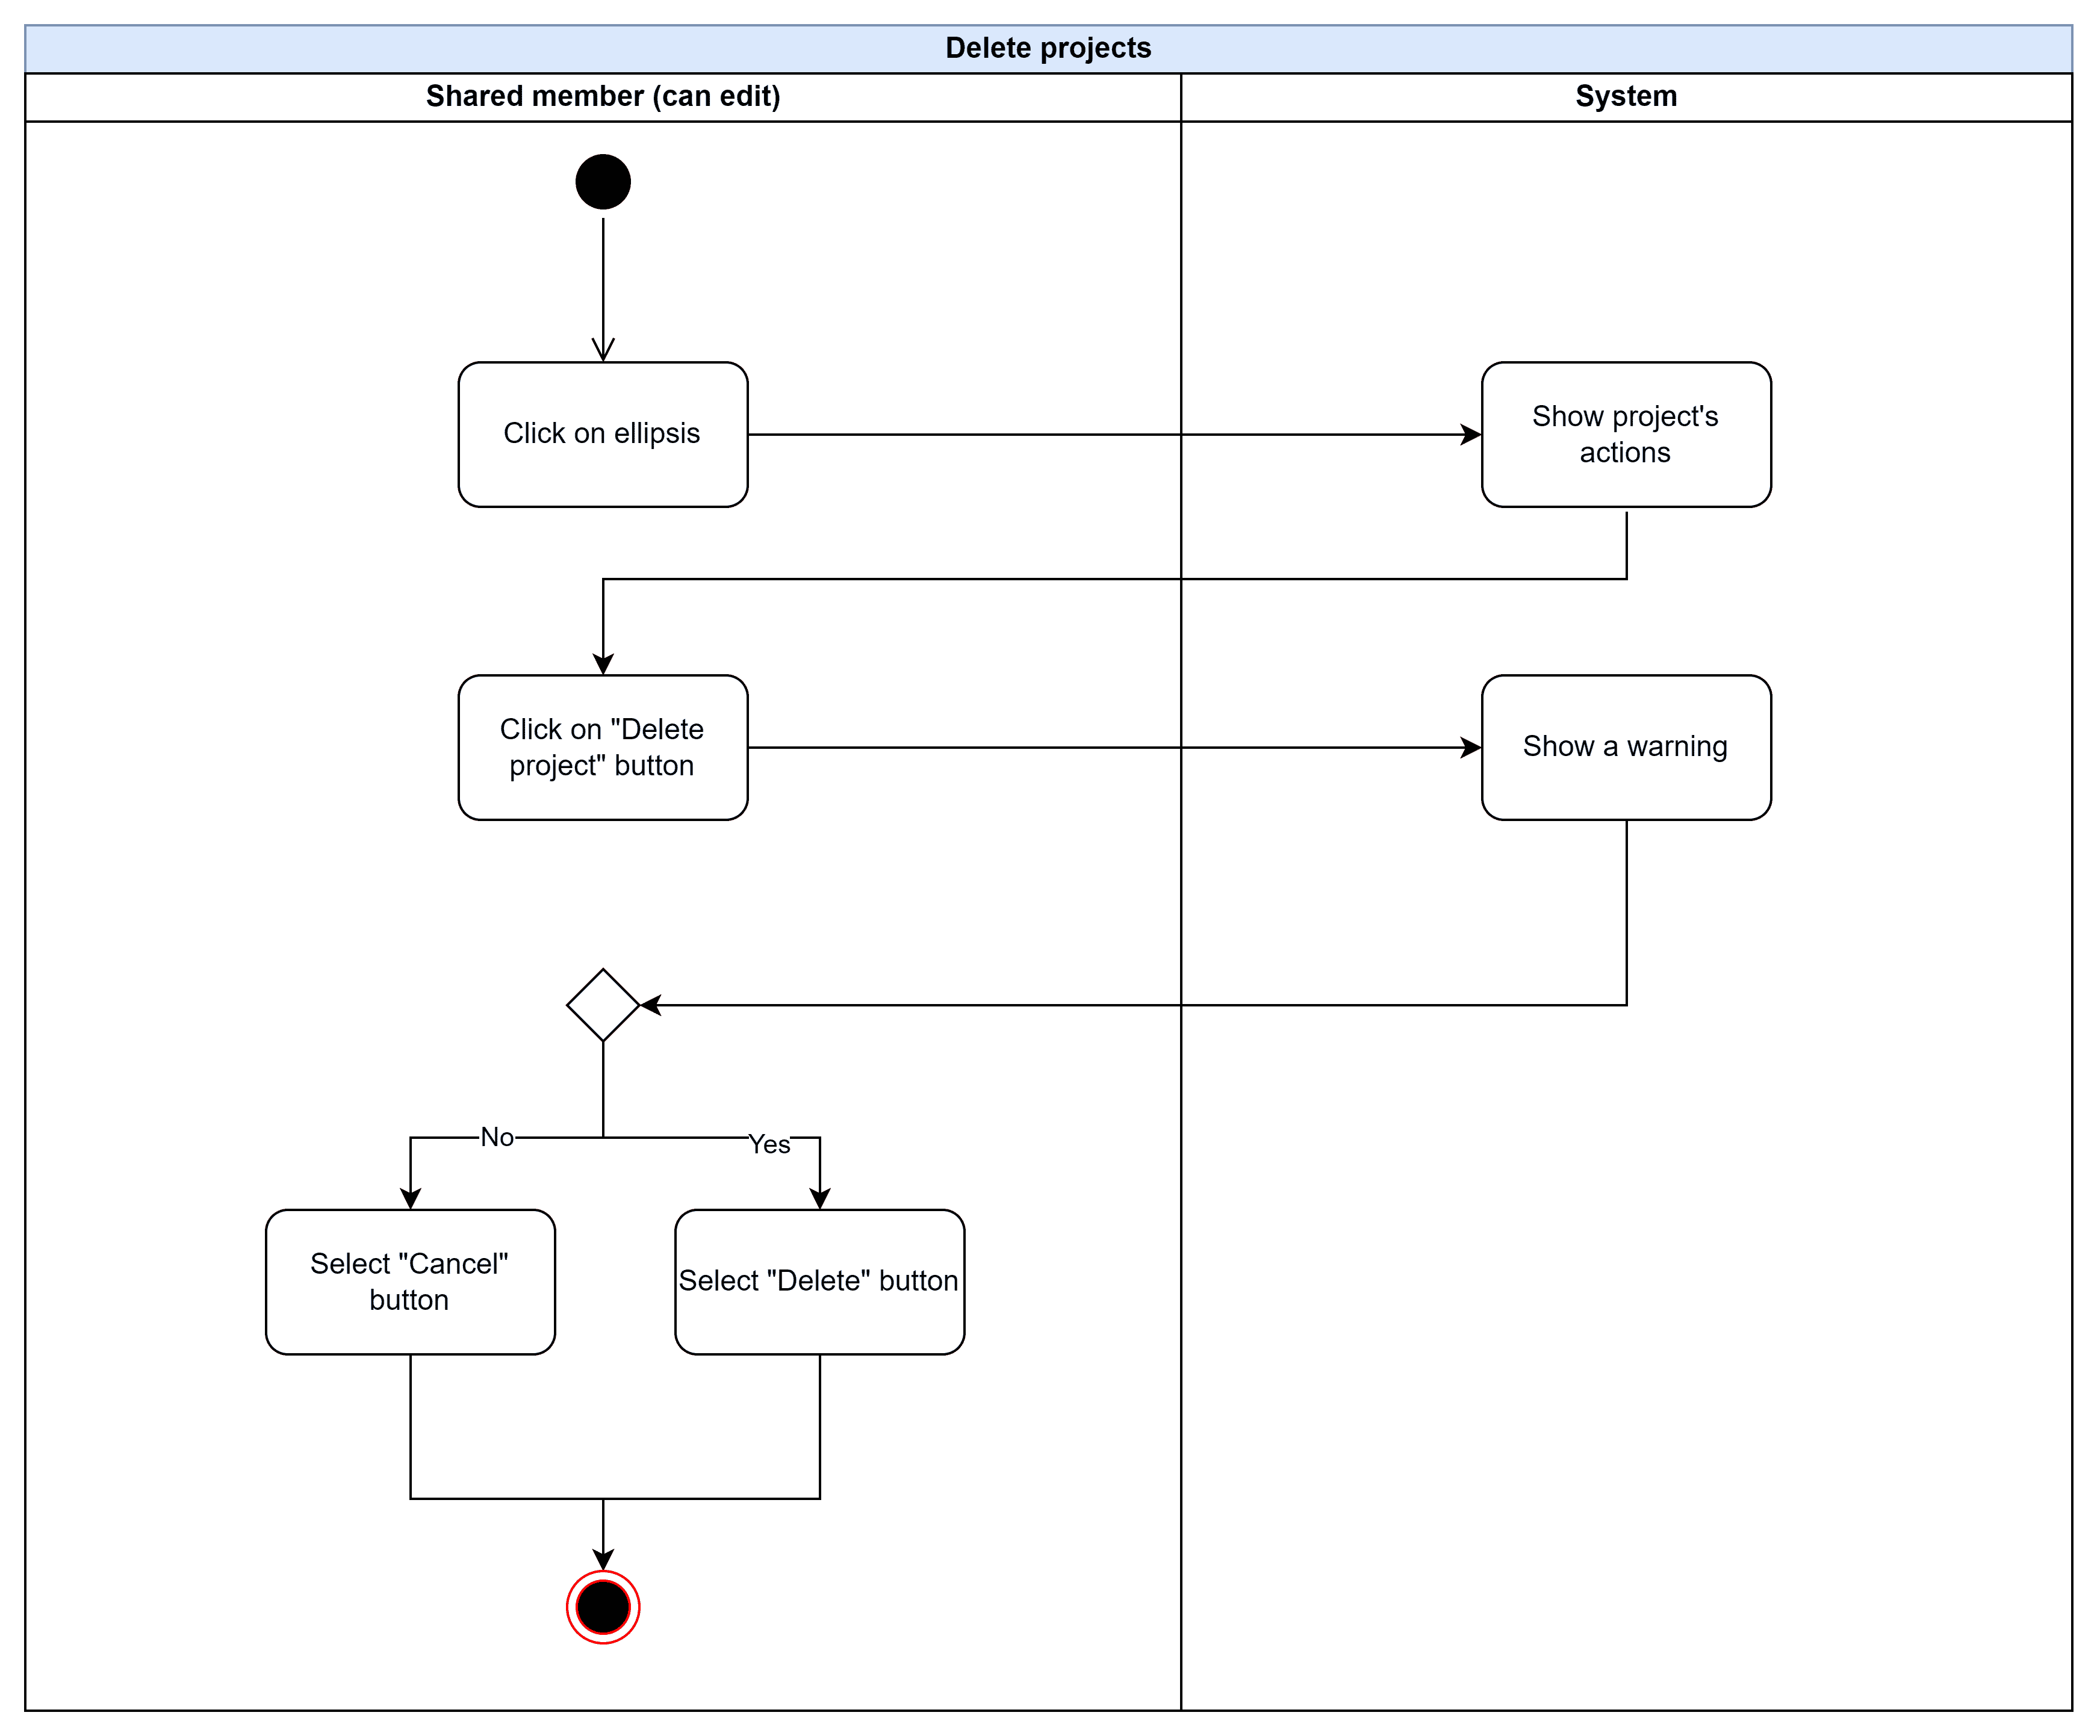
\includegraphics[width=\linewidth]{Content/Phân tích và thiết kế hệ thống/documents/Sơ đồ hoạt động/images/deleteProjects.png}
        \vspace{0.5cm}
        \caption{Xoá project trong Workspace}
        \label{fig:Xoá project trong Workspace}
    \end{figure}

\newpage
\subsection{Gửi lời mời trực tiếp đến cho user}
    \begin{figure}[H]
        \centering
        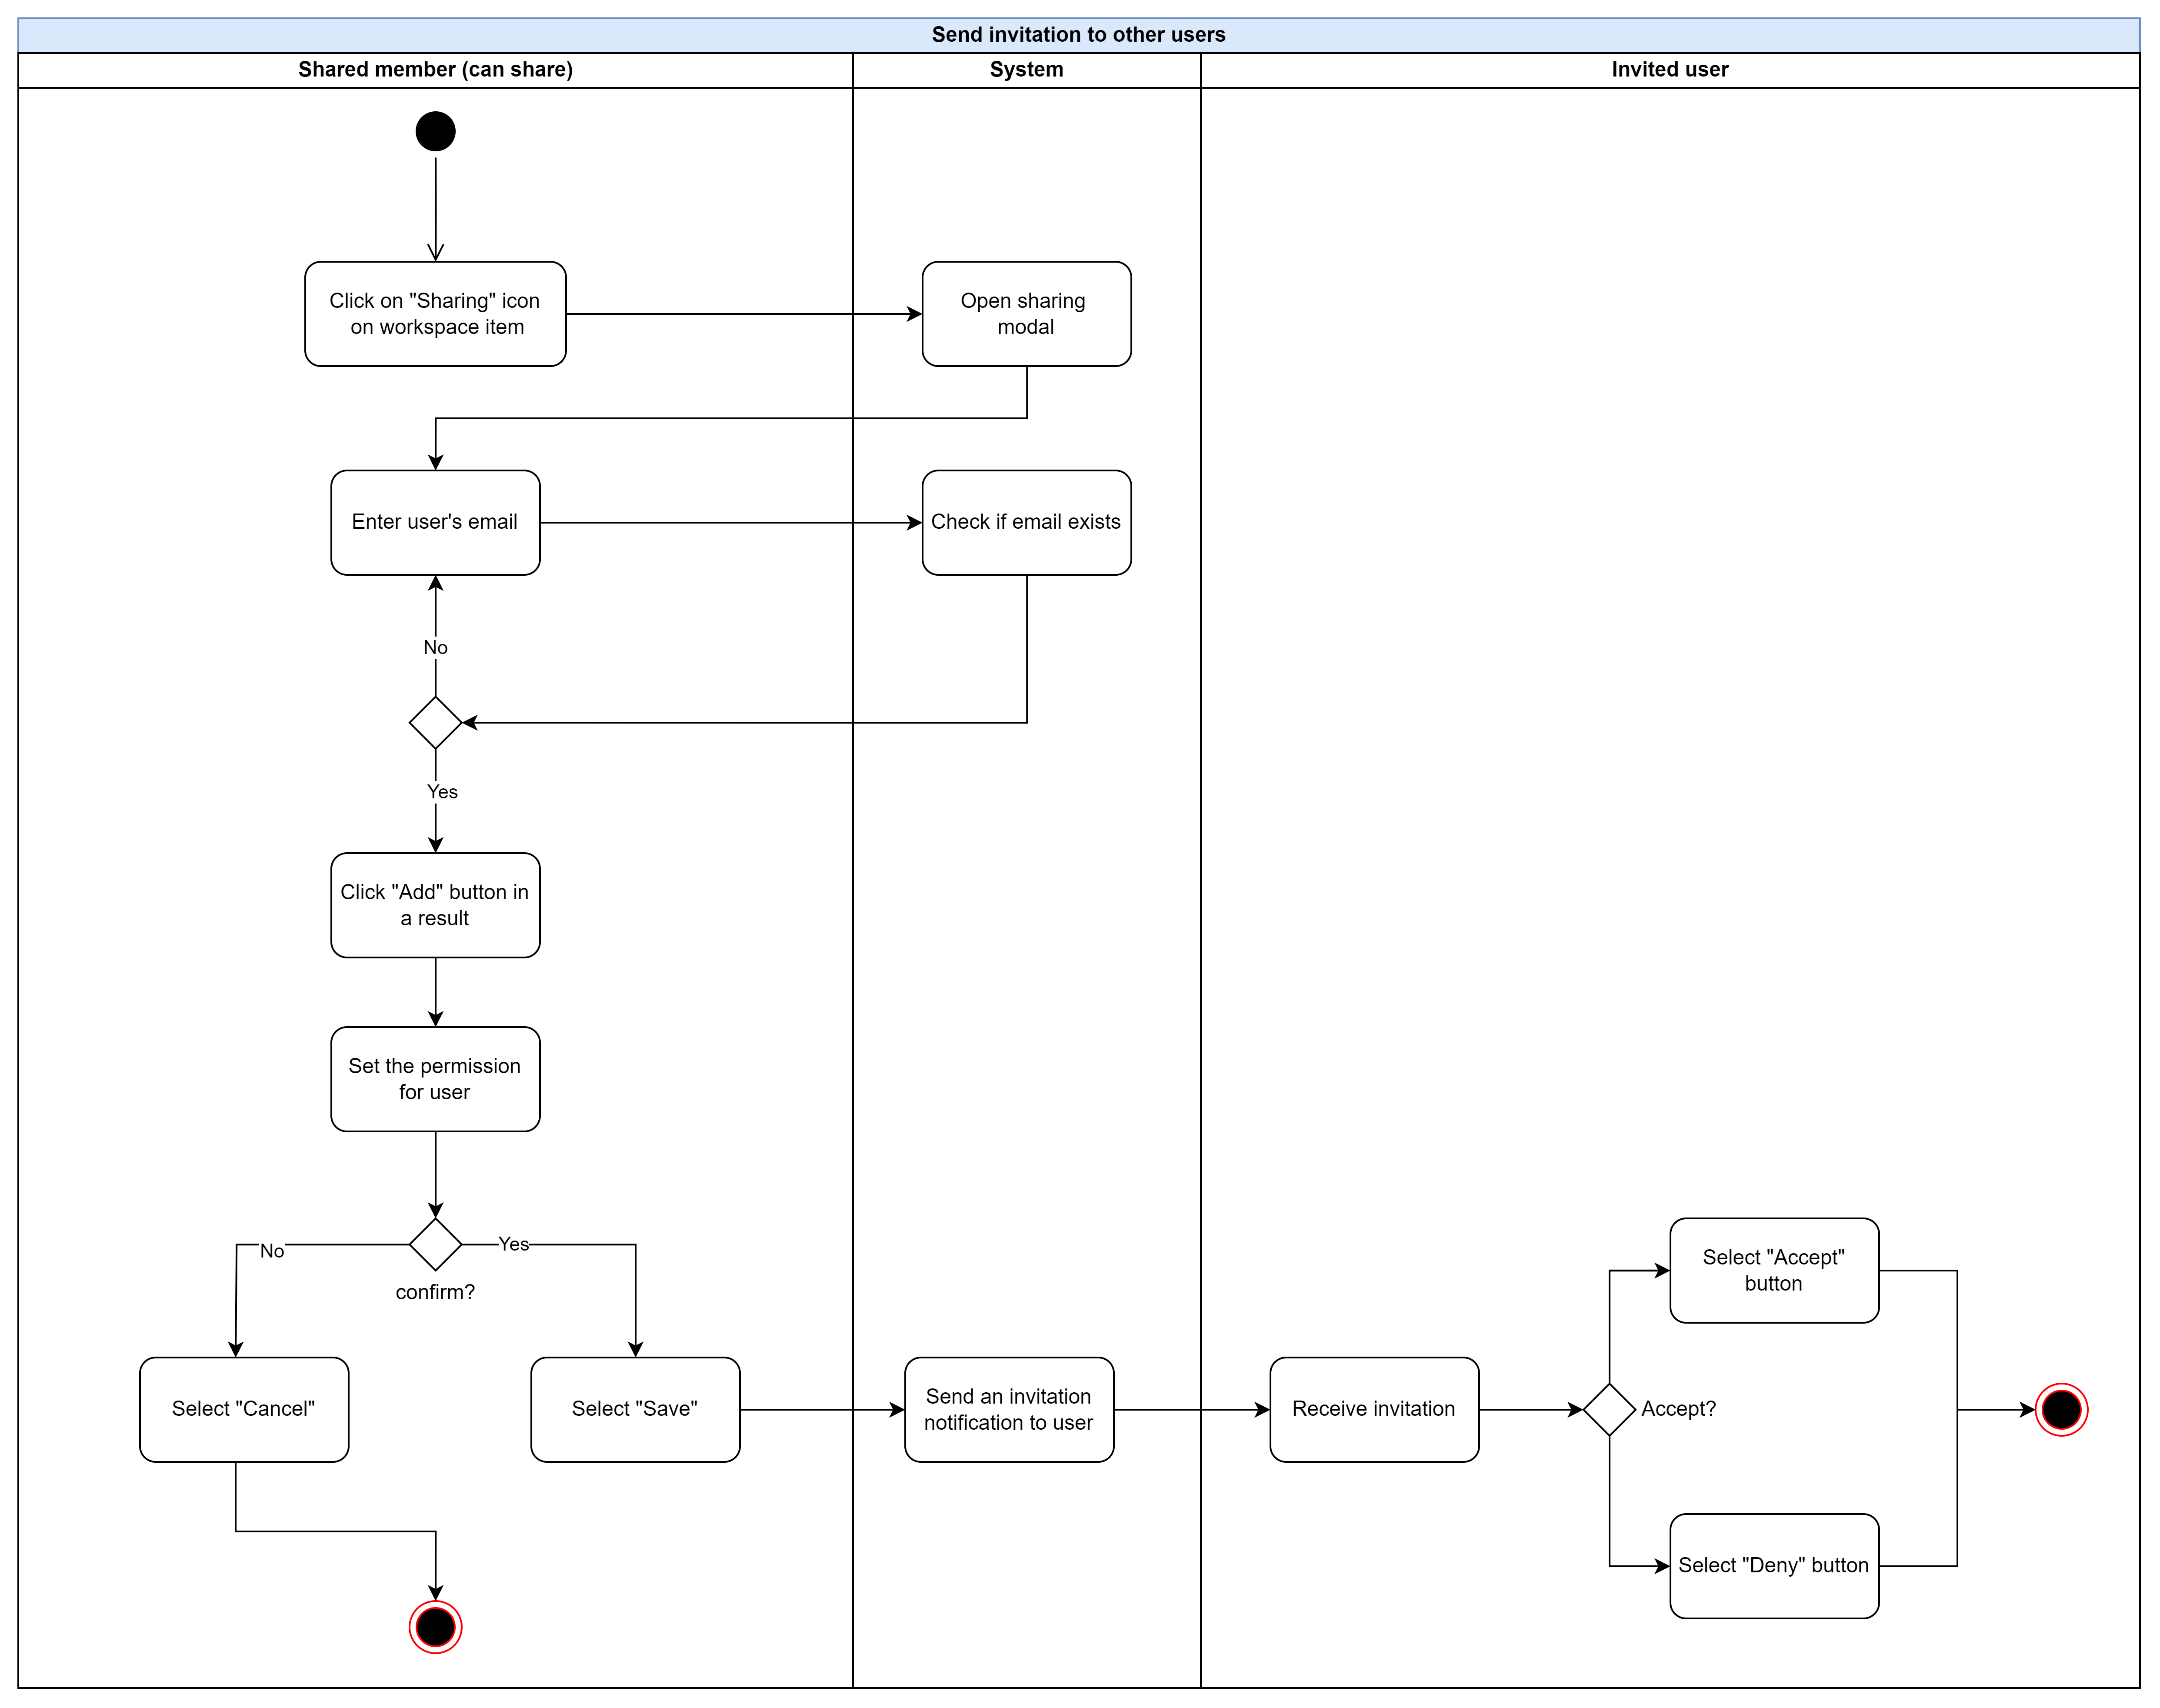
\includegraphics[width=\linewidth]{Content/Phân tích và thiết kế hệ thống/documents/Sơ đồ hoạt động/images/sendInvitation.png}
        \vspace{0.5cm}
        \caption{Gửi lời mời trực tiếp đến cho user}
        \label{fig:Gửi lời mời trực tiếp đến cho user}
    \end{figure}

\newpage
\subsection{Gửi yêu cầu đổi quyền truy cập Workspace}
    \begin{figure}[H]
        \centering
        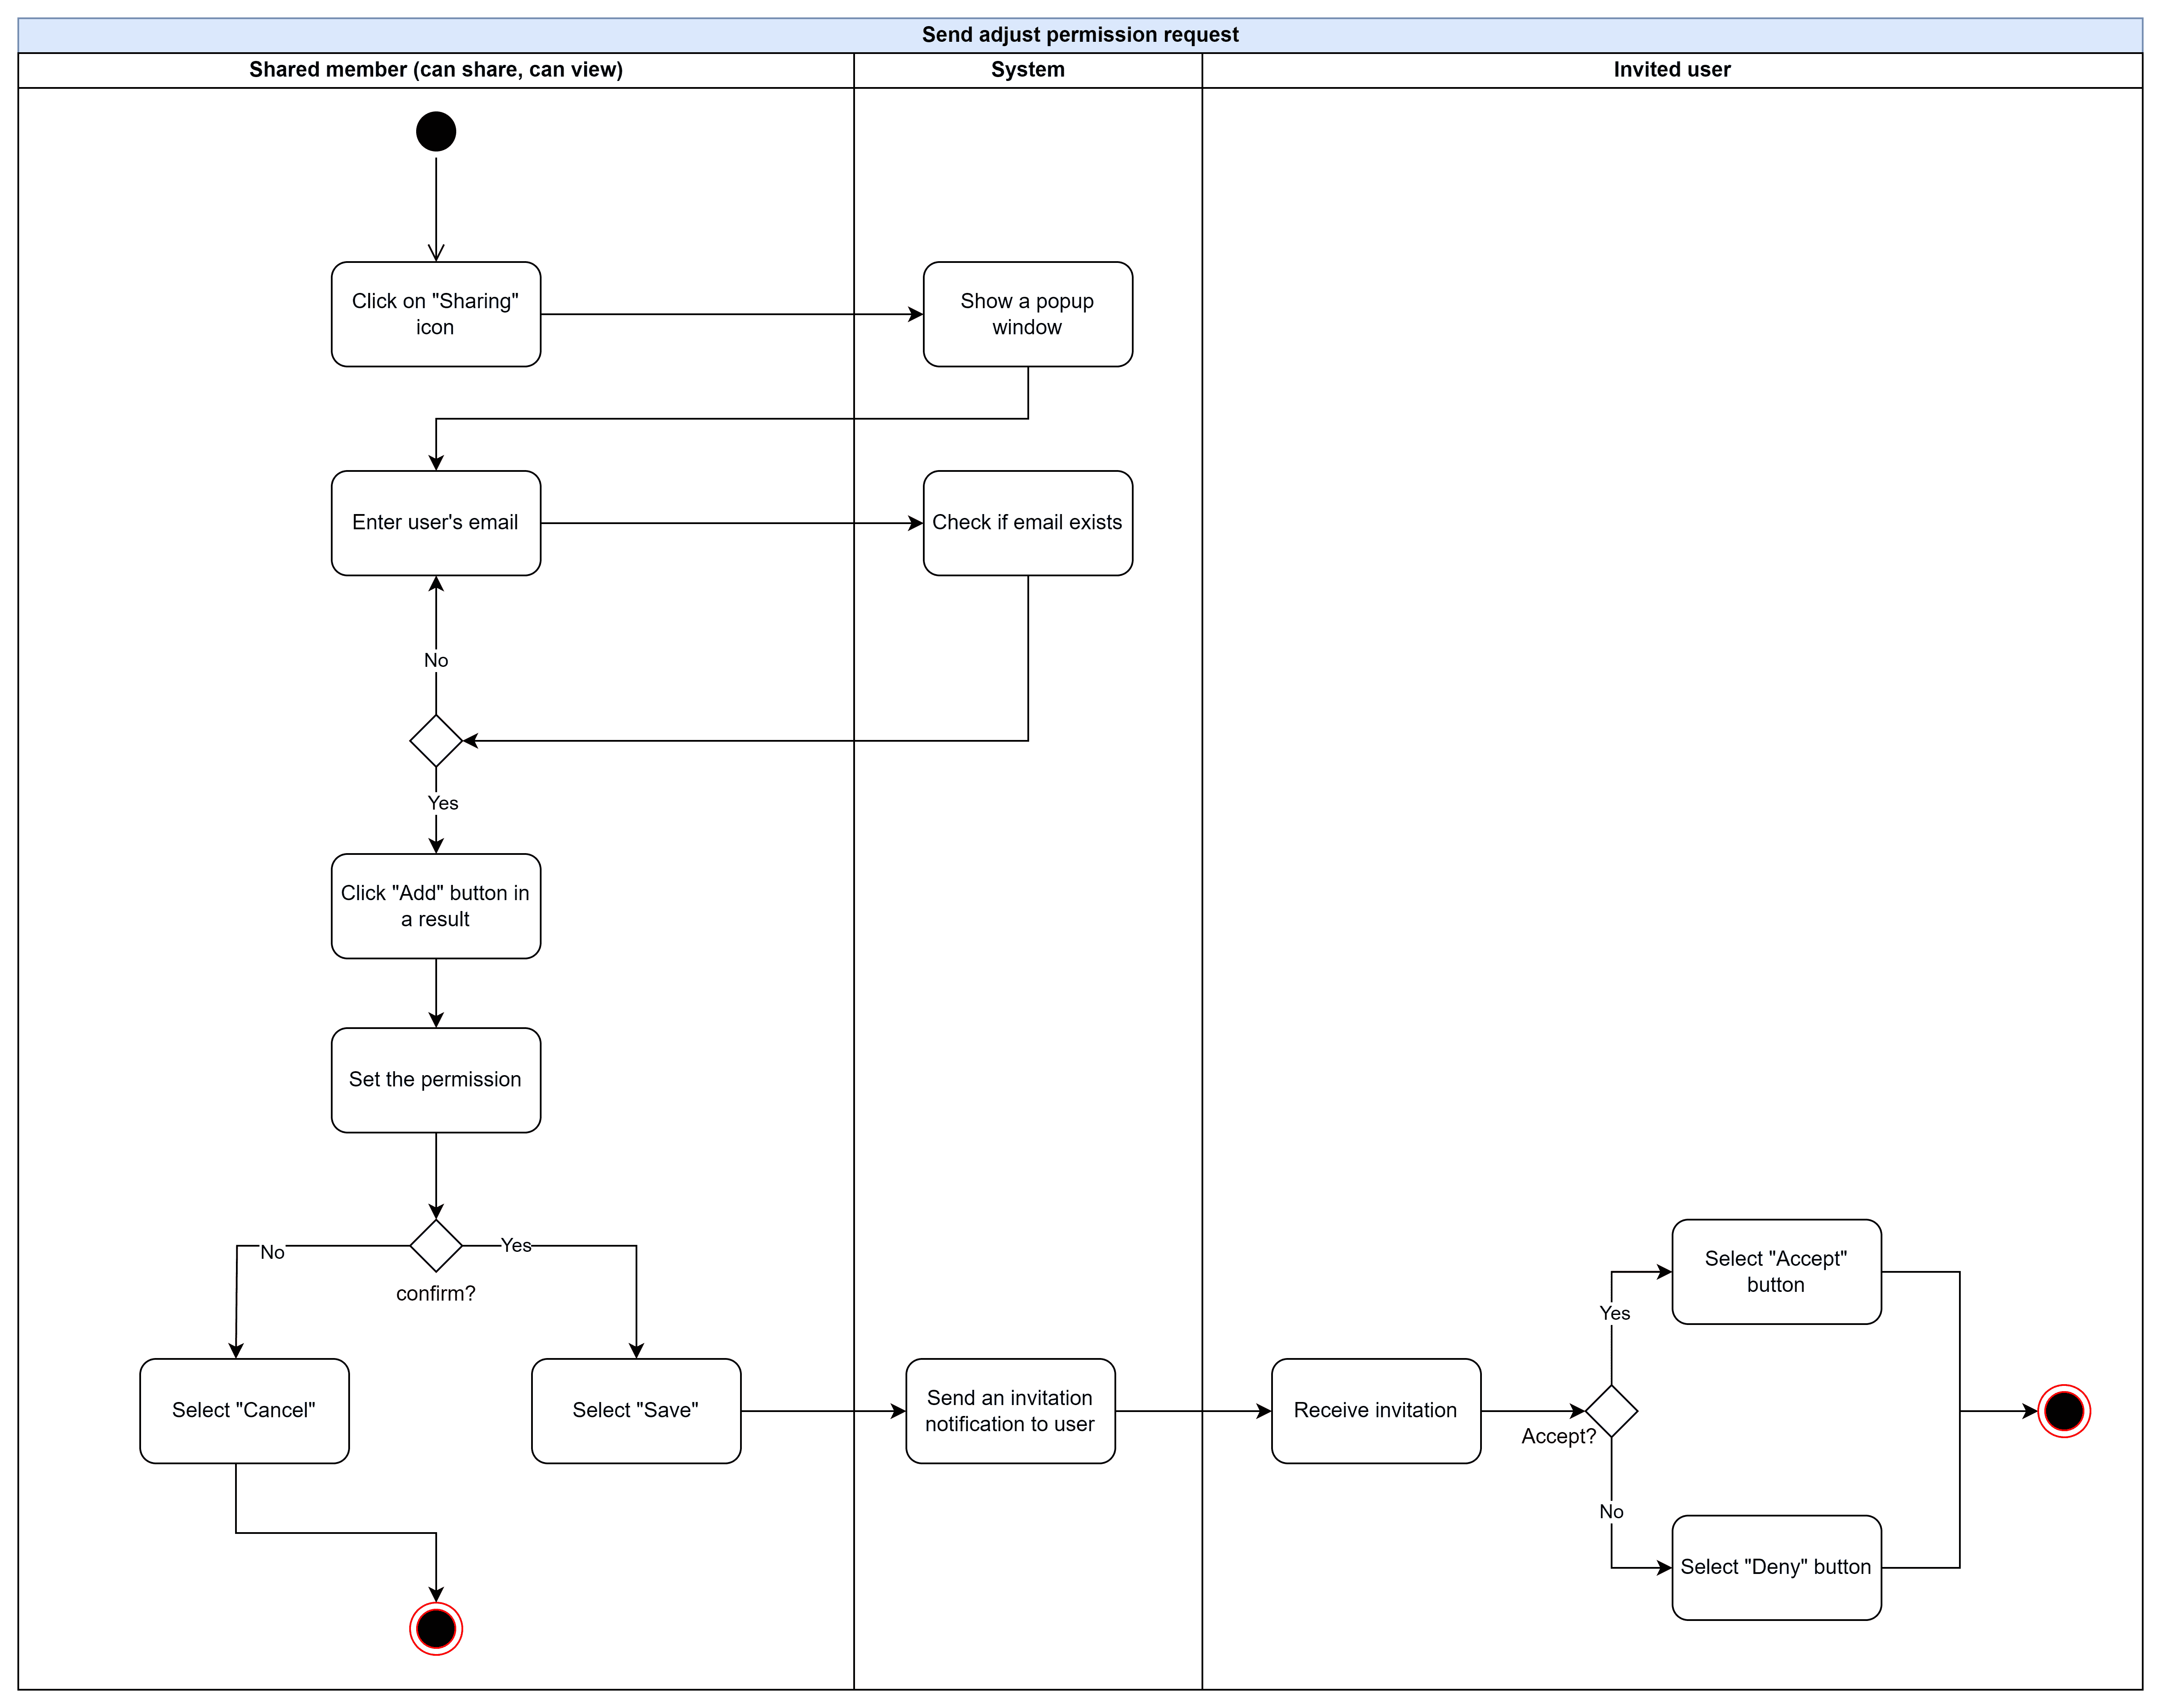
\includegraphics[width=\linewidth]{Content/Phân tích và thiết kế hệ thống/documents/Sơ đồ hoạt động/images/sendAdjustPermissionRequest.png}
        \vspace{0.5cm}
        \caption{Gửi yêu cầu đổi quyền truy cập Workspace}
        \label{fig:Gửi yêu cầu đổi quyền truy cập Workspace}
    \end{figure}

\newpage
\subsection{Gửi yêu cầu mời người dùng tham gia Workspace}
    \begin{figure}[H]
        \centering
        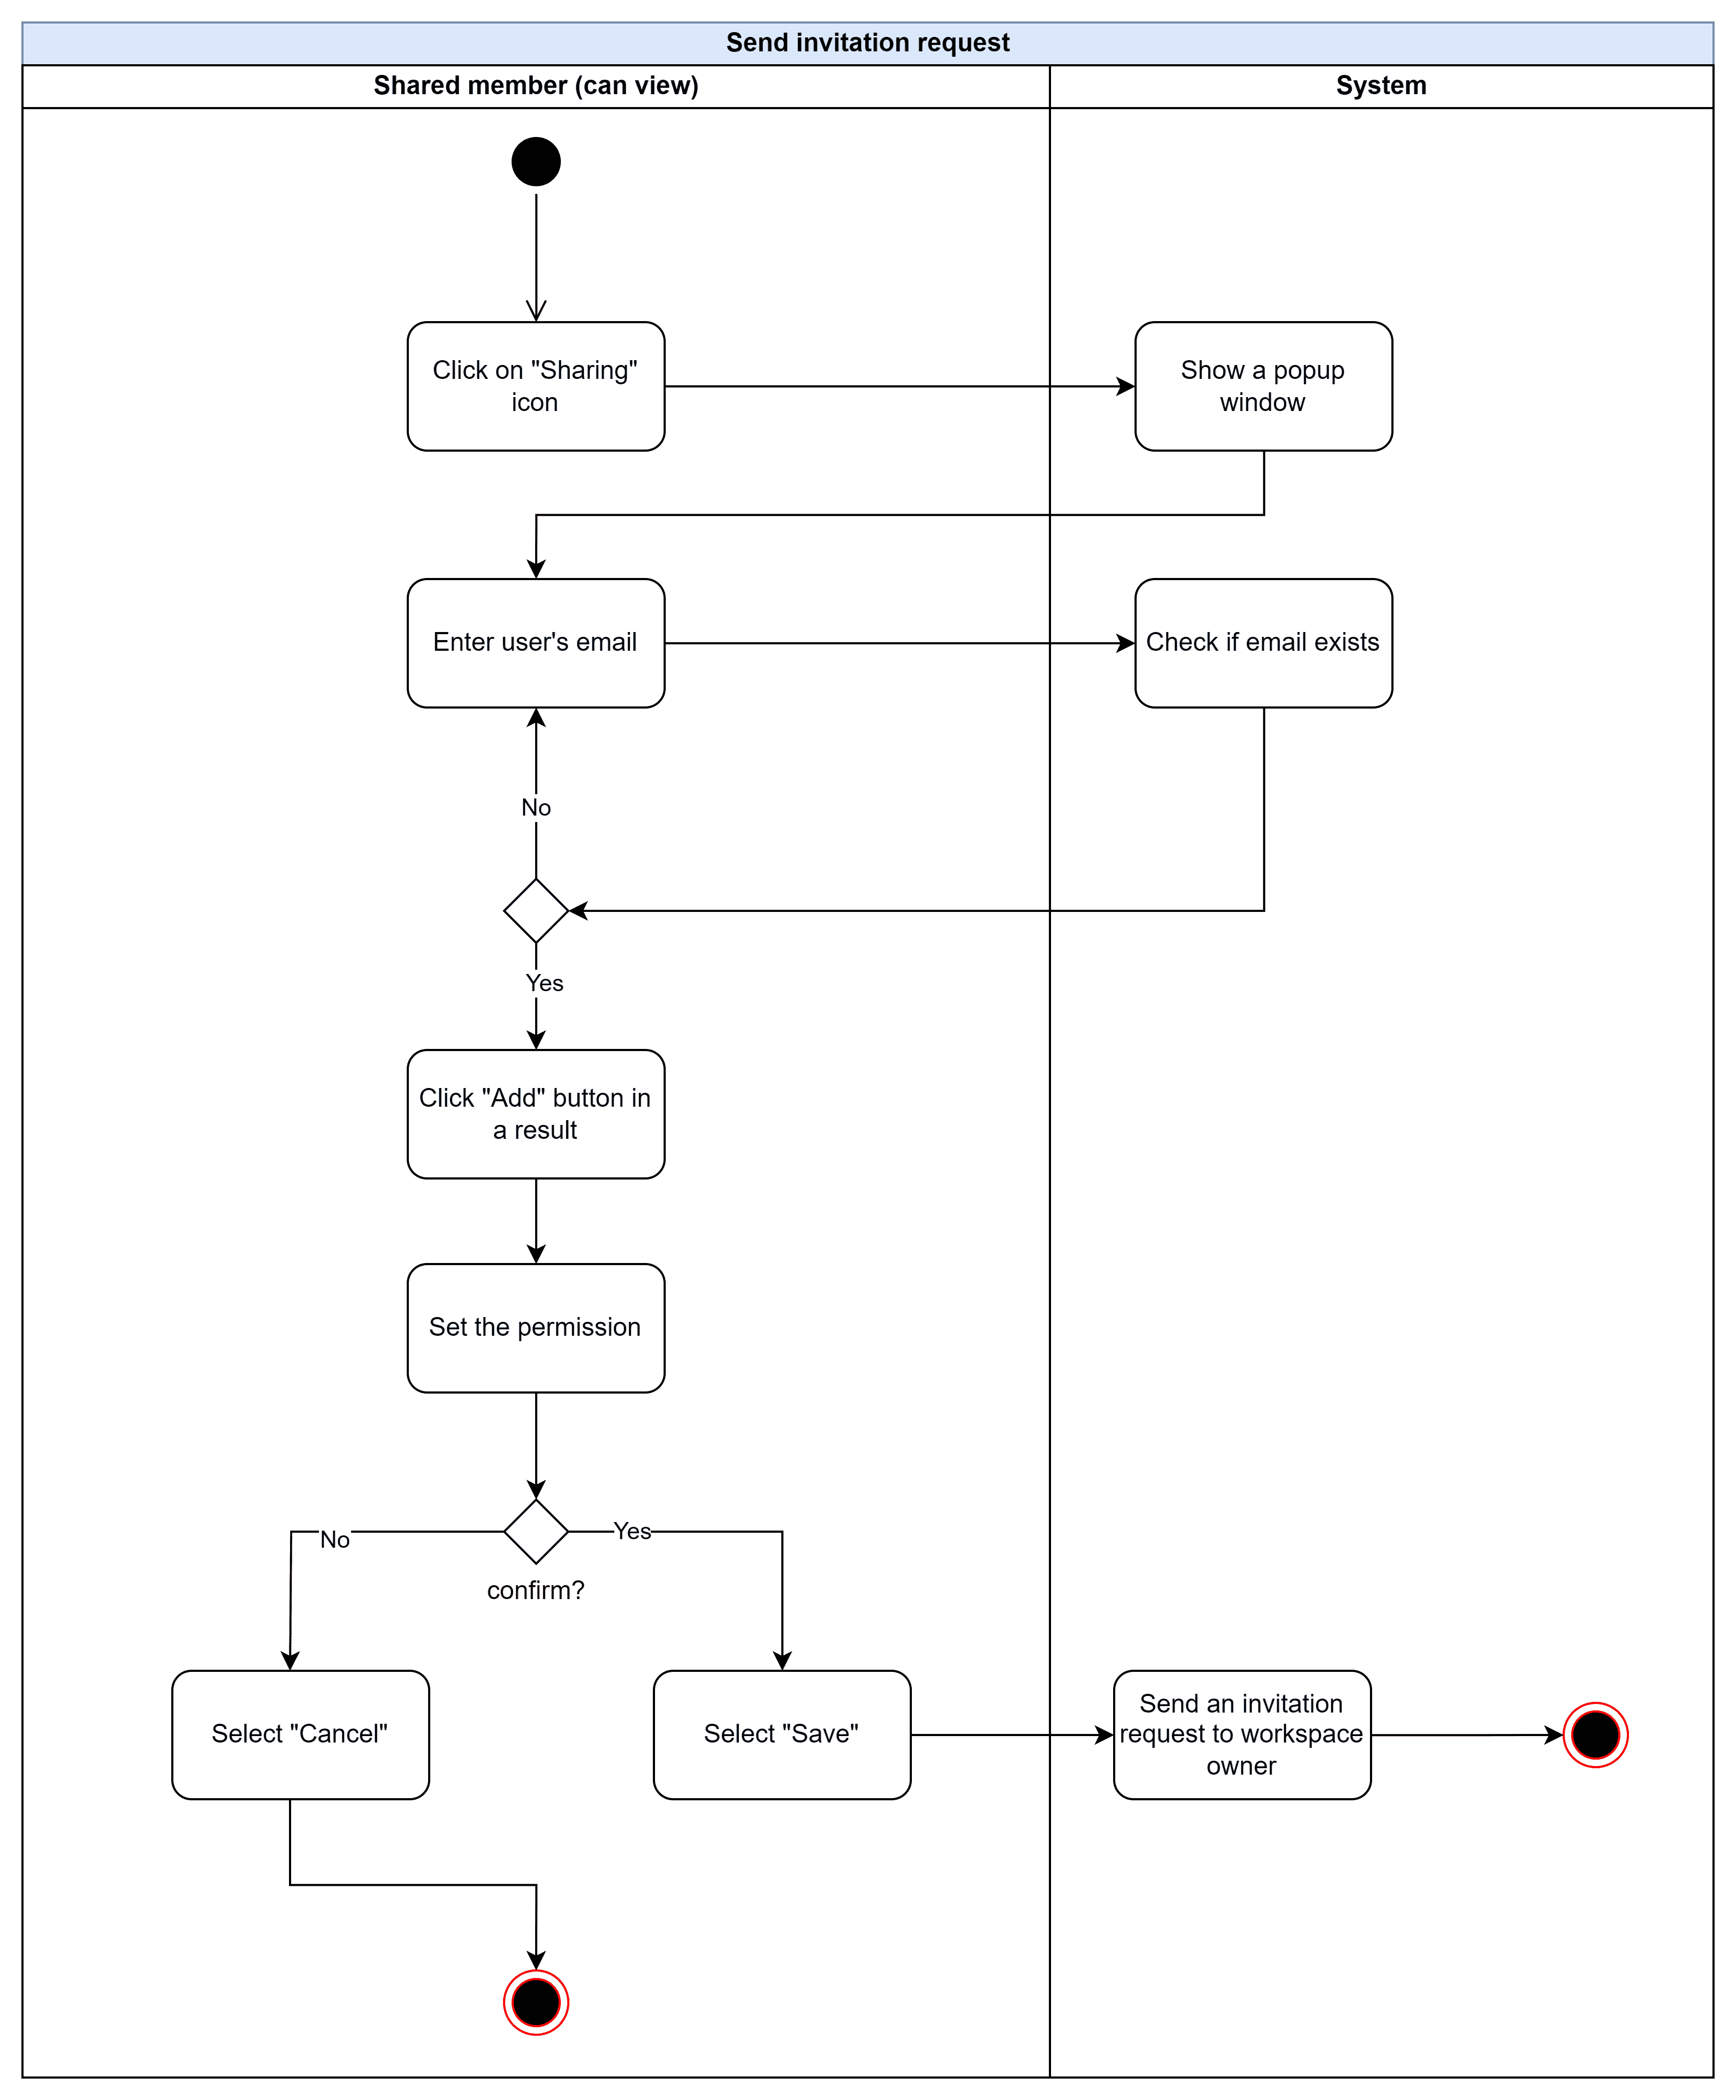
\includegraphics[width=\linewidth]{Content/Phân tích và thiết kế hệ thống/documents/Sơ đồ hoạt động/images/sendInvitationRequest.png}
        \vspace{0.5cm}
        \caption{Gửi yêu cầu mời người dùng tham gia Workspace}
        \label{fig:Gửi yêu cầu mời người dùng tham gia Workspace}
    \end{figure}

\newpage
\subsection{Mở trang thông báo của người dùng}
    \begin{figure}[H]
        \centering
        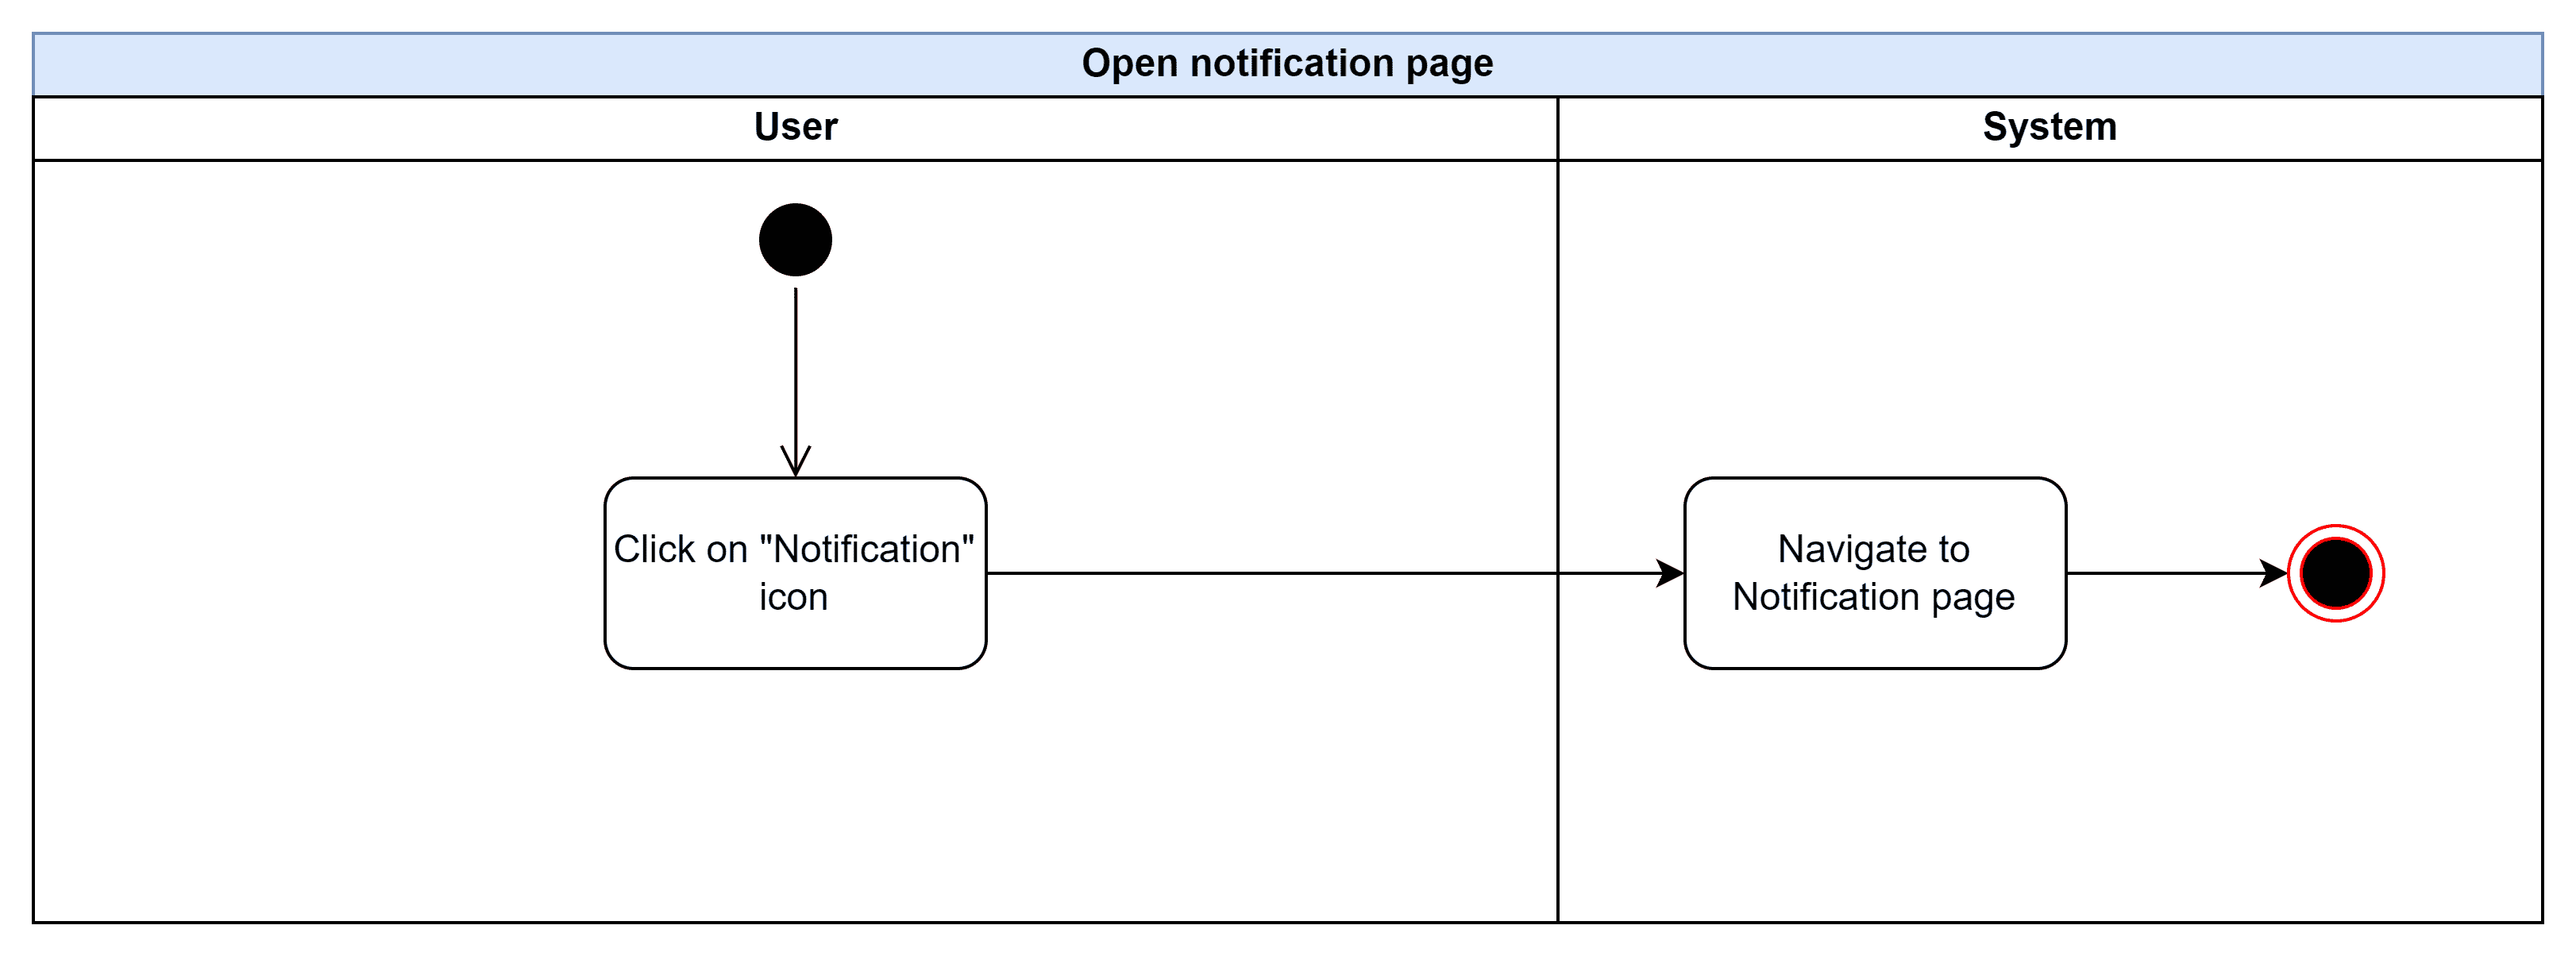
\includegraphics[width=\linewidth]{Content/Phân tích và thiết kế hệ thống/documents/Sơ đồ hoạt động/images/openNotificationPage.png}
        \vspace{0.5cm}
        \caption{Mở trang thông báo của người dùng}
        \label{fig:Mở trang thông báo của người dùng}
    \end{figure}

\newpage
\subsubsection{Xem chi tiết thông báo}
    \begin{figure}[H]
        \centering
        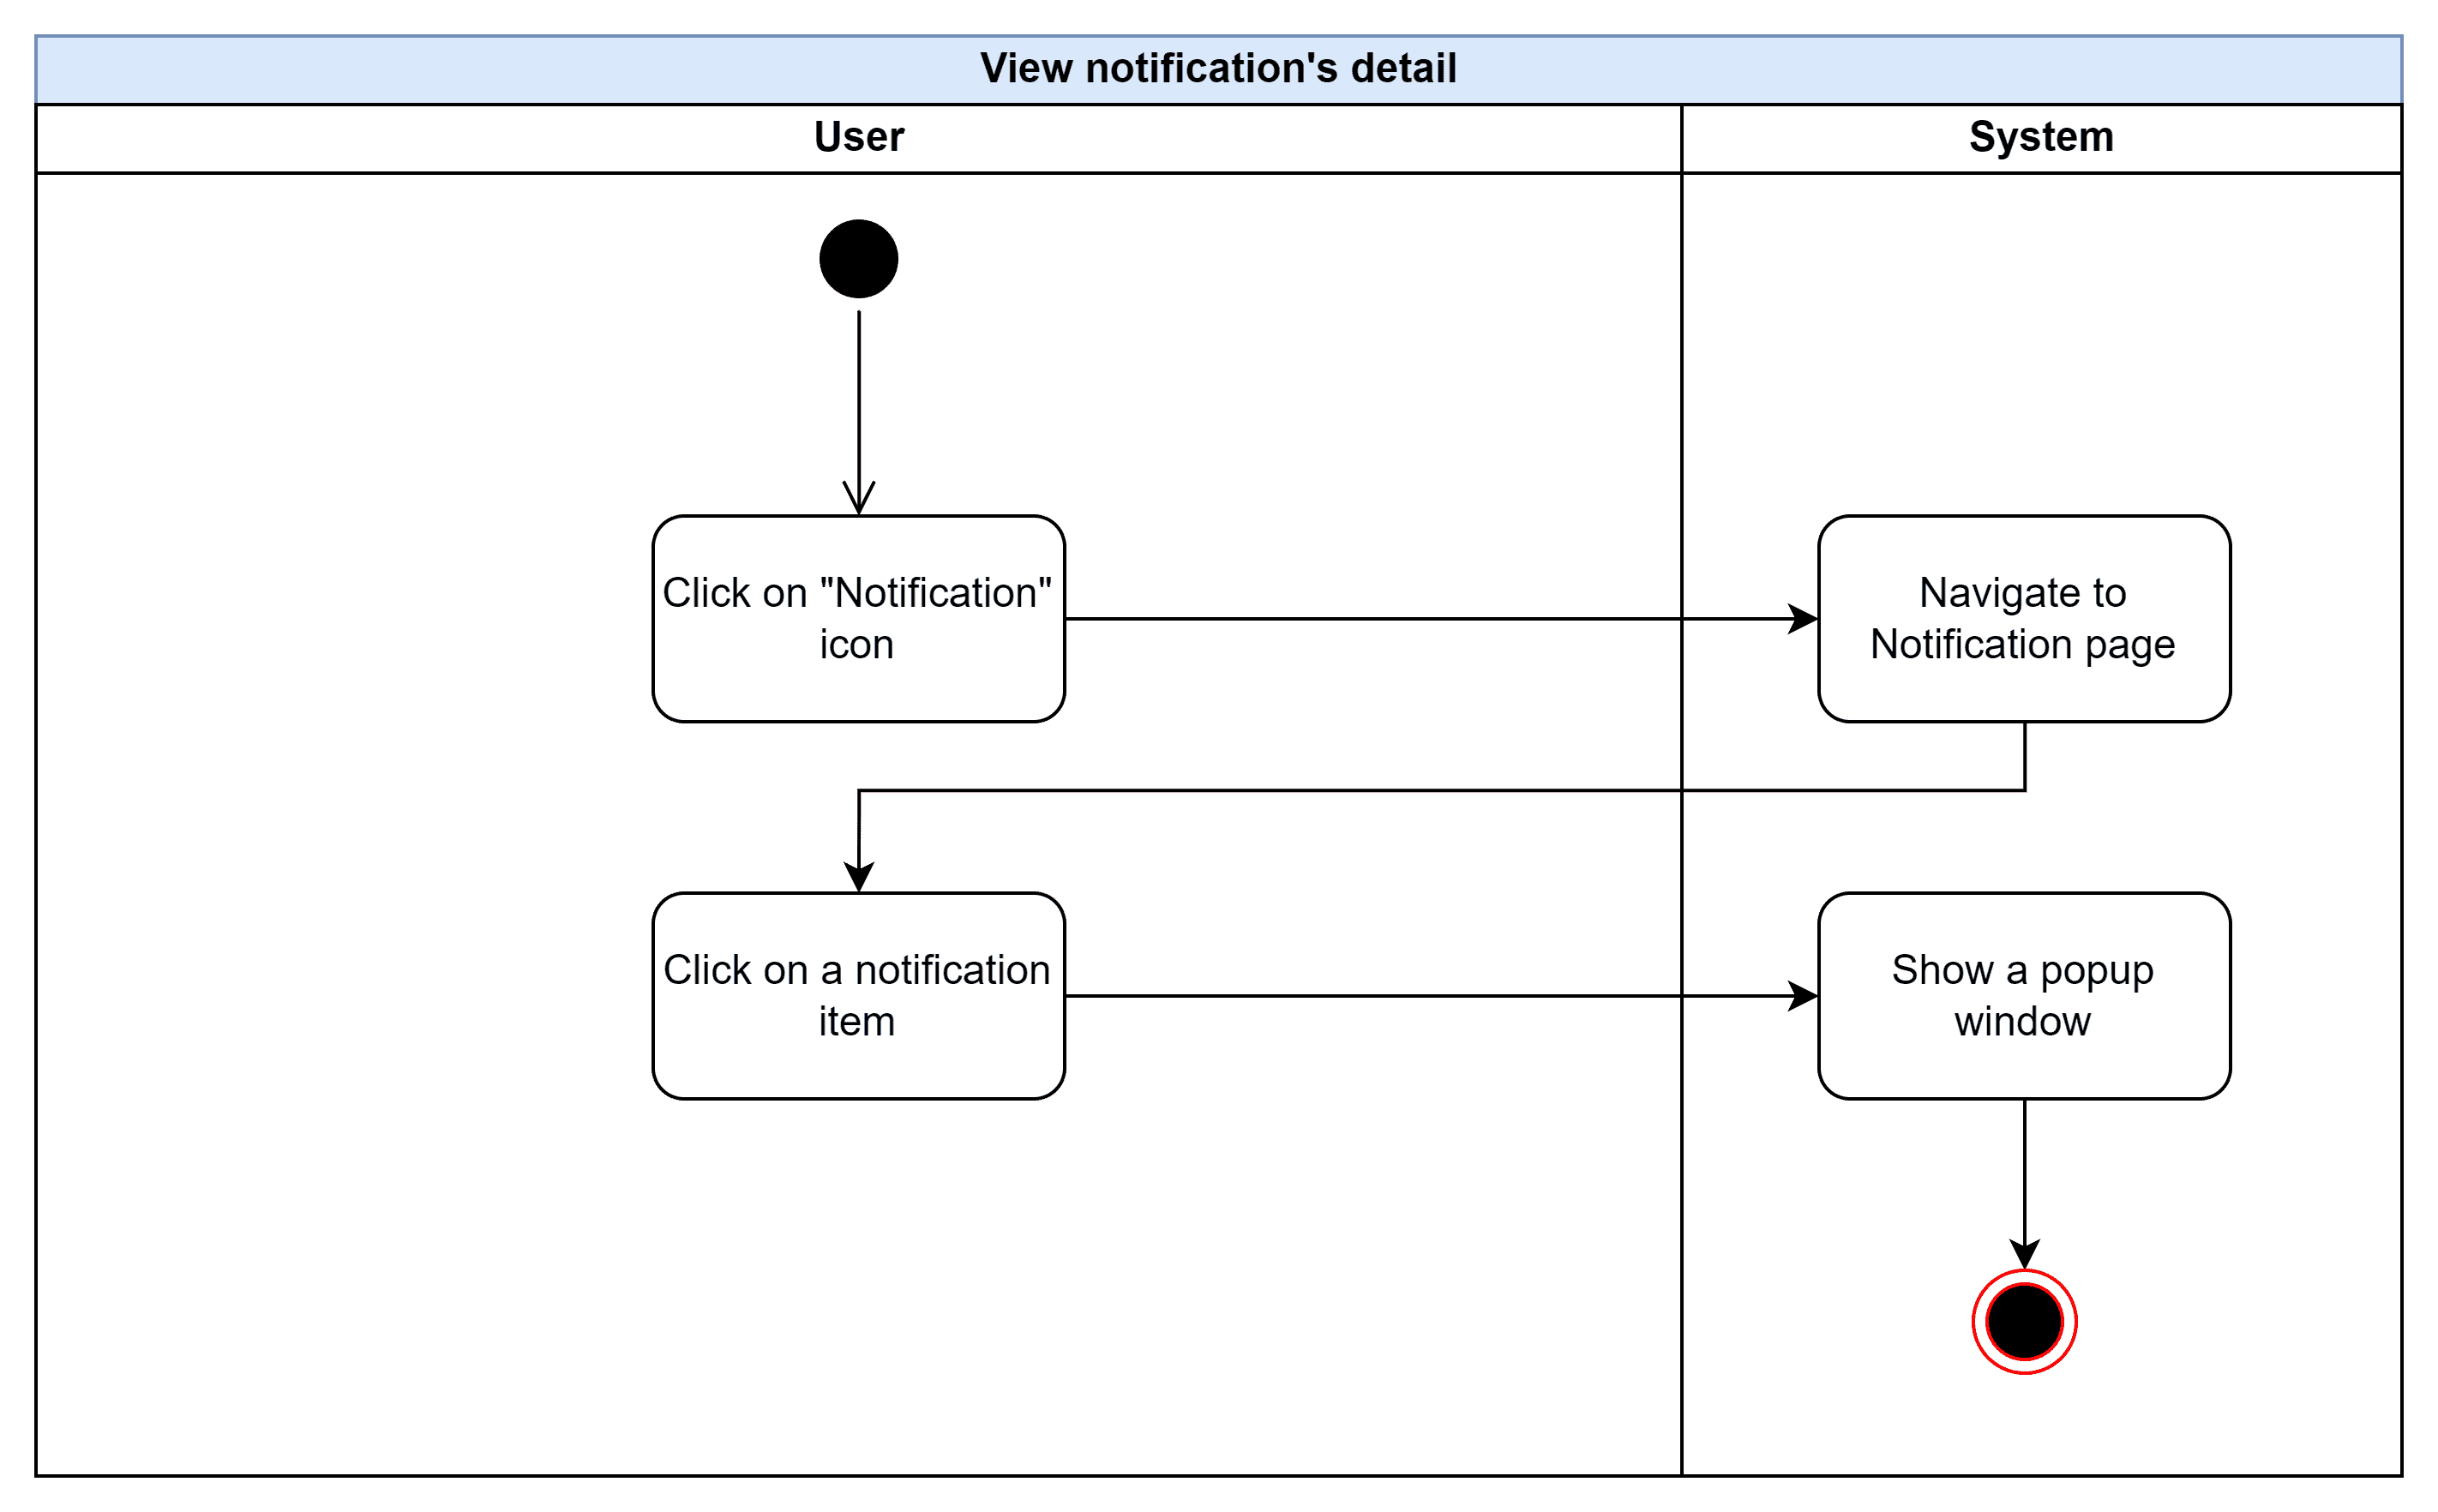
\includegraphics[width=\linewidth]{Content/Phân tích và thiết kế hệ thống/documents/Sơ đồ hoạt động/images/viewNotificationDetail.png}
        \vspace{0.5cm}
        \caption{Xem chi tiết thông báo}
        \label{fig:Xem chi tiết thông báo}
    \end{figure}

\newpage
\subsubsection{Xoá thông báo}
    \begin{figure}[H]
        \centering
        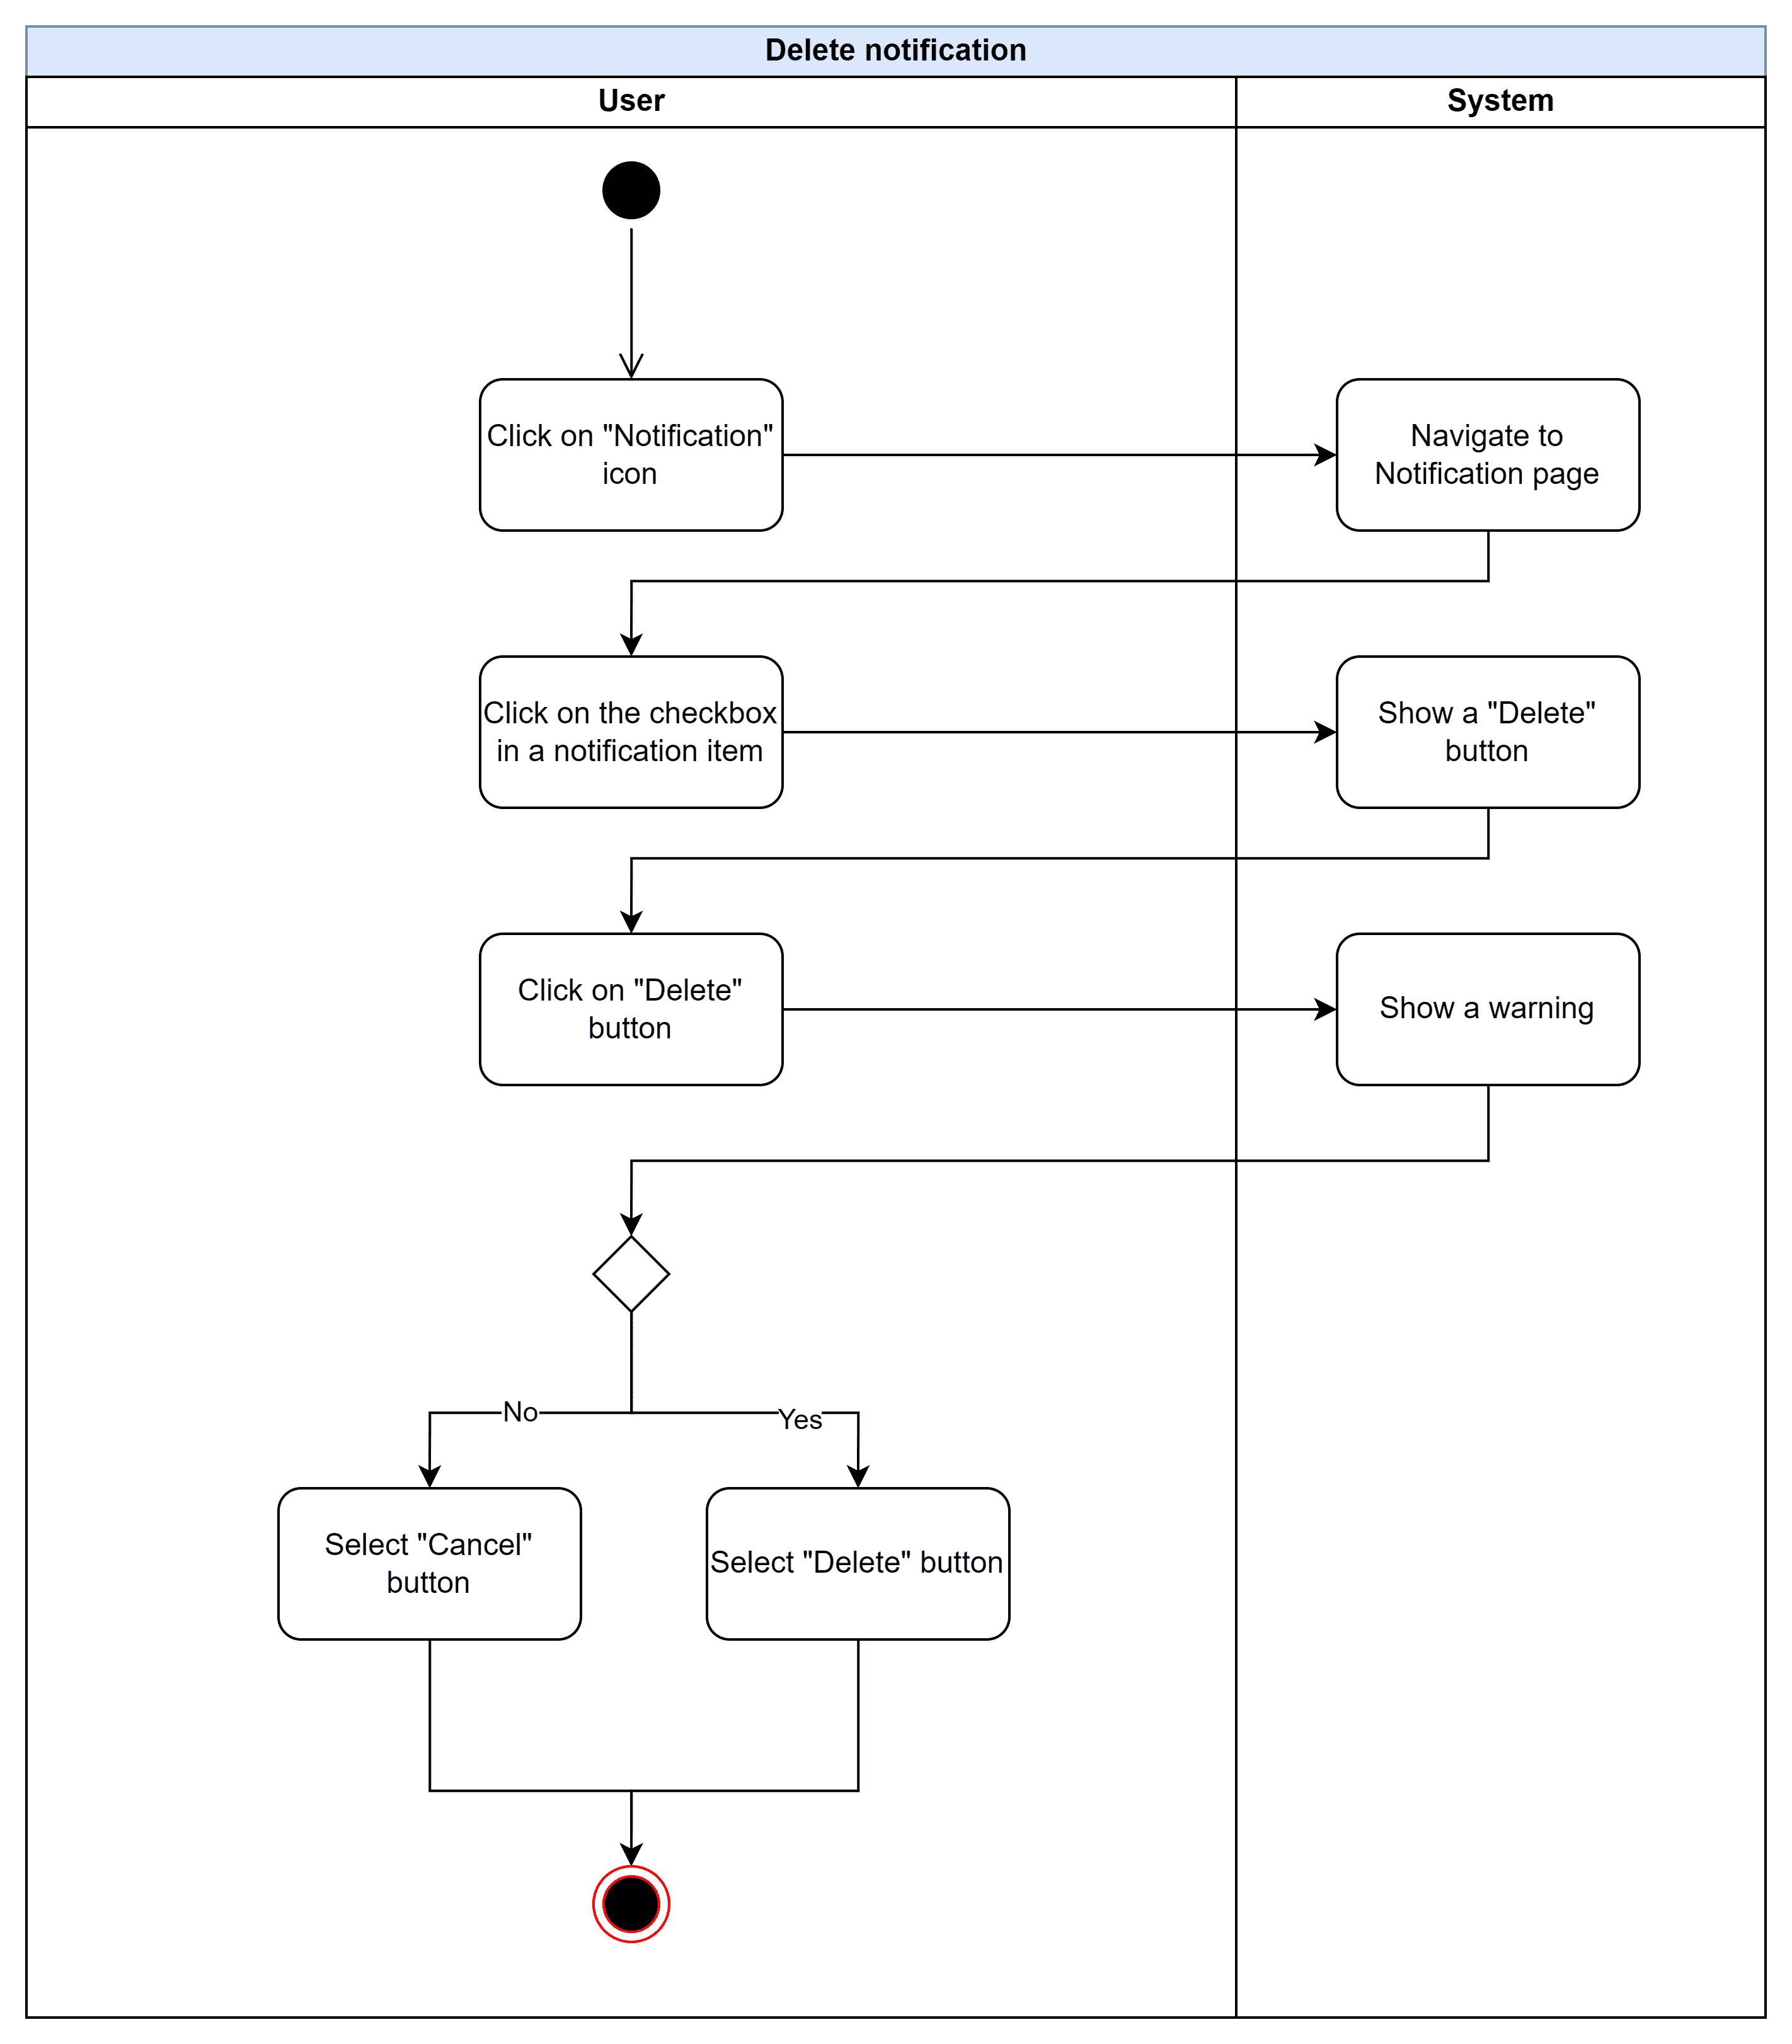
\includegraphics[width=\linewidth]{Content/Phân tích và thiết kế hệ thống/documents/Sơ đồ hoạt động/images/deleteNotification.png}
        \vspace{0.5cm}
        \caption{Xoá thông báo}
        \label{fig:Xoá thông báo}
    \end{figure}

\newpage
\subsubsection{Đánh dấu thông báo}
\begin{figure}[H]
    \centering
    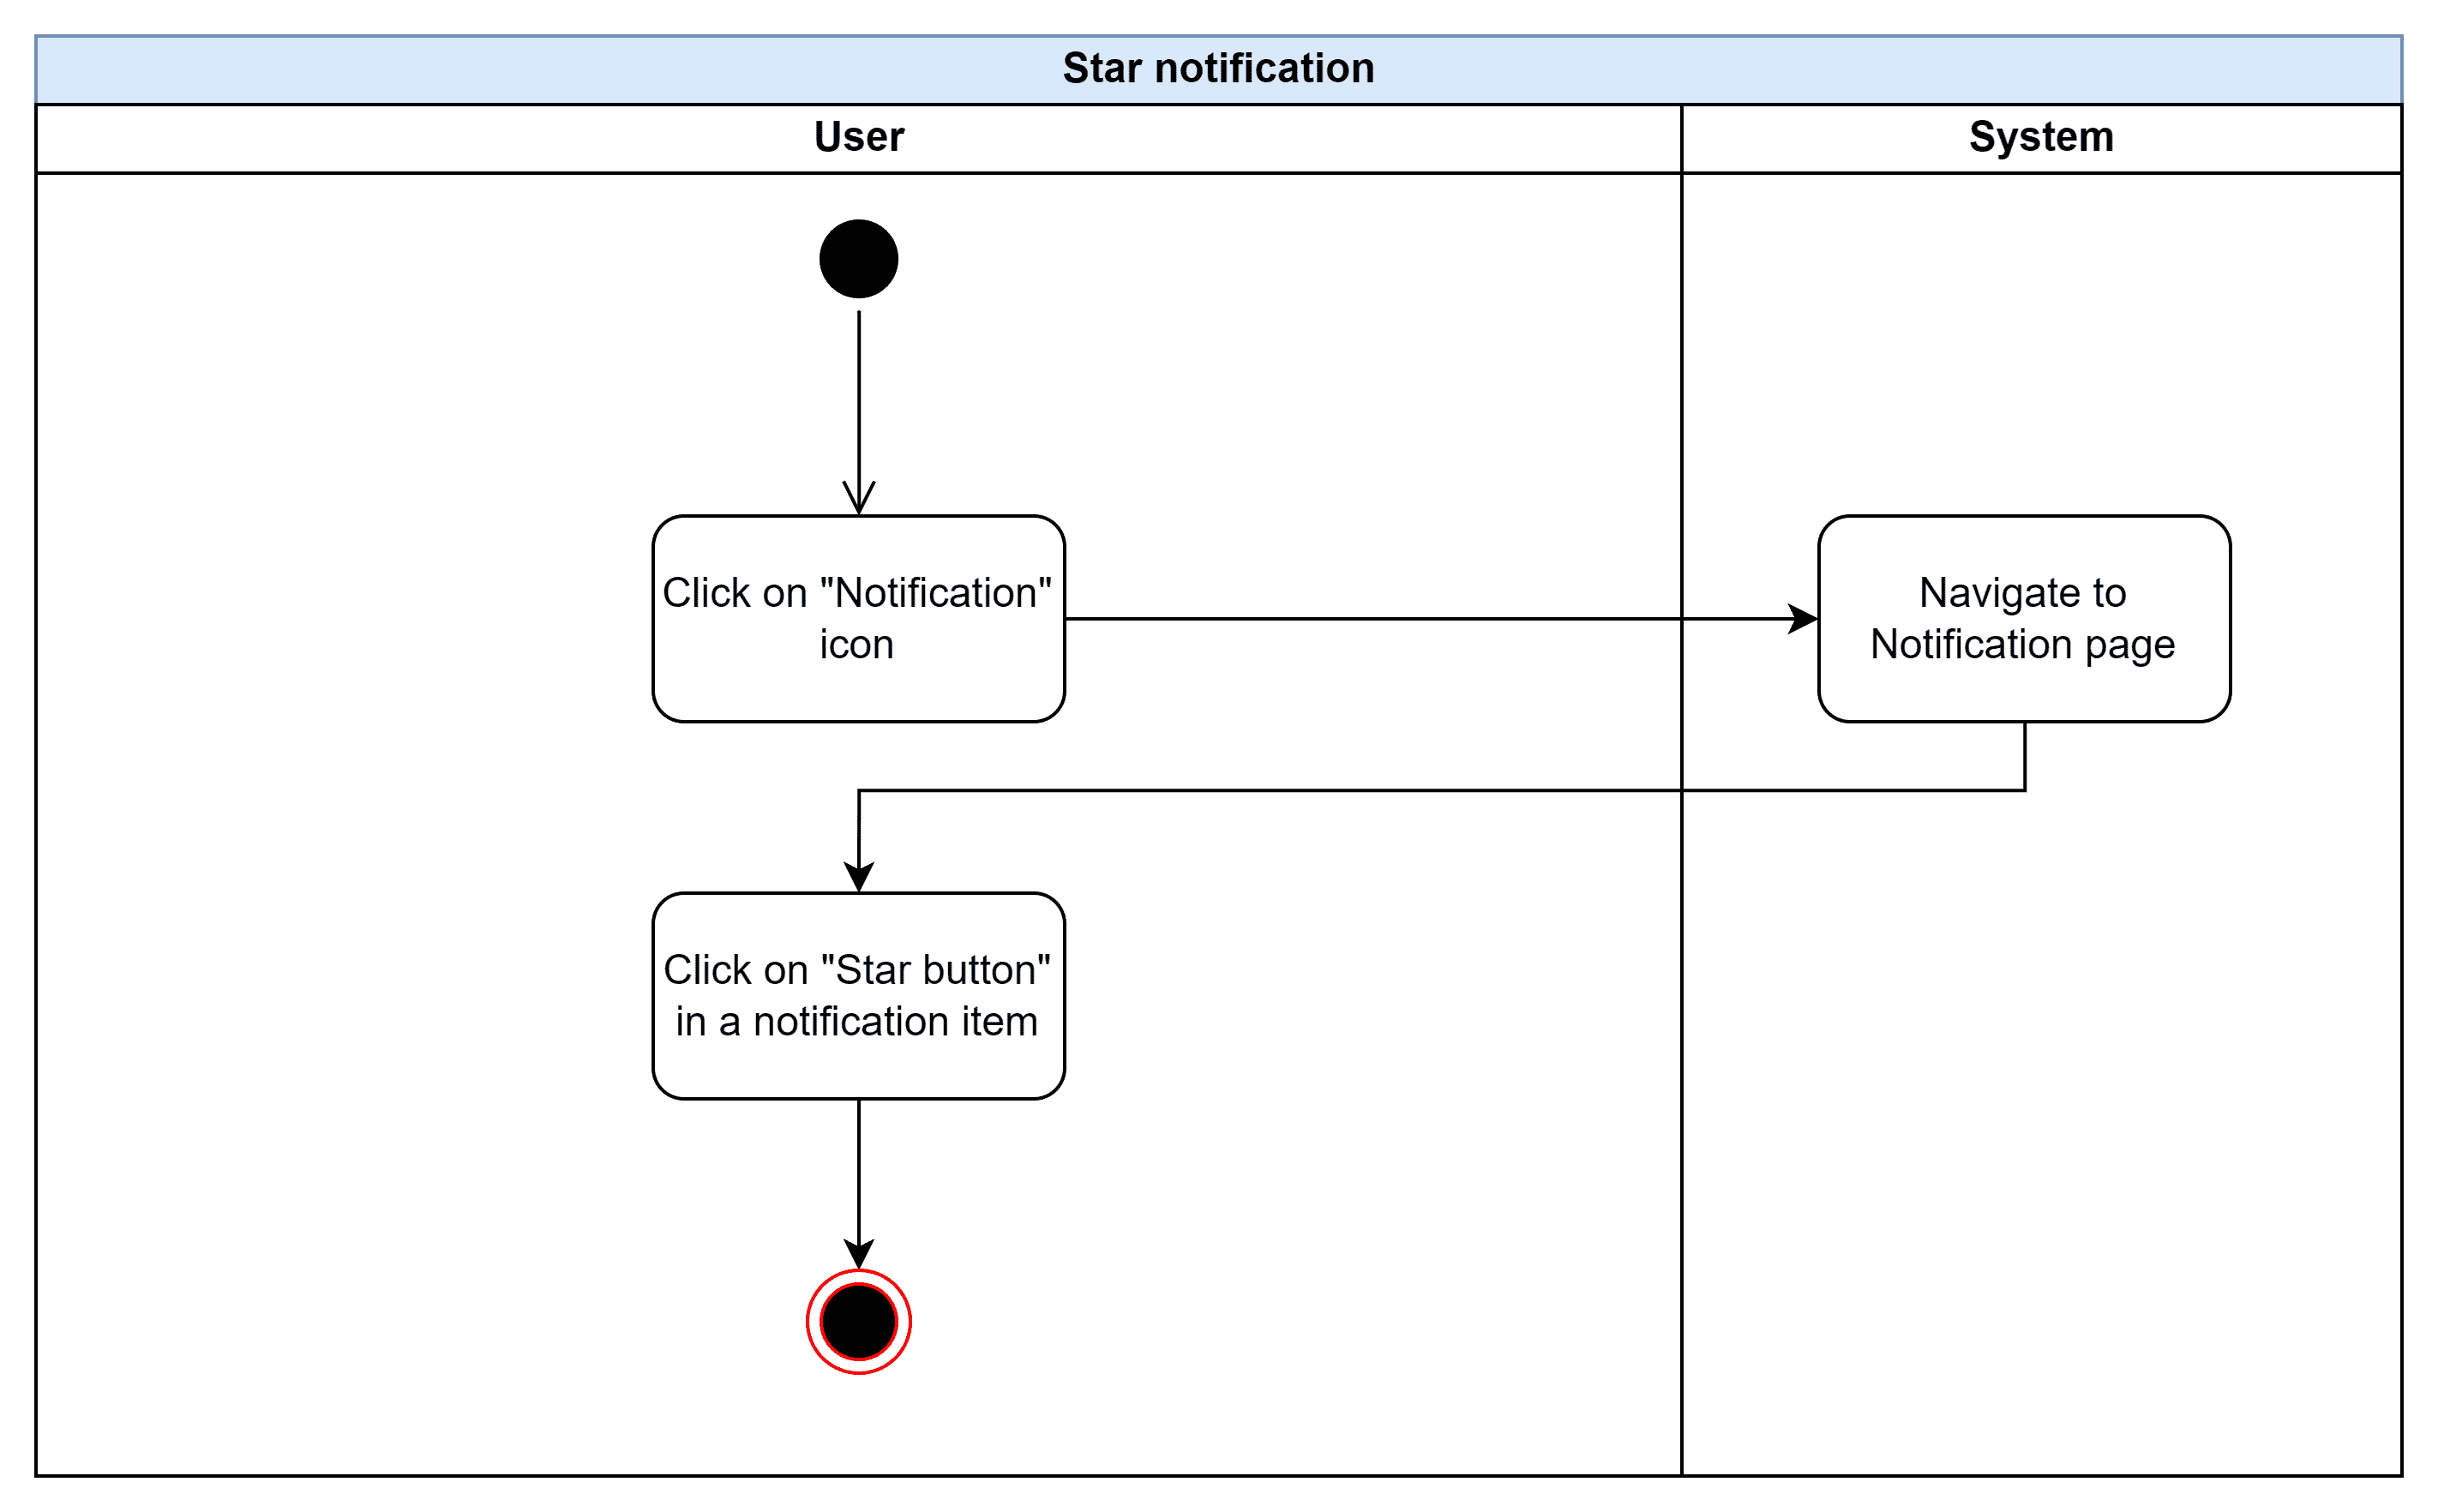
\includegraphics[width=\linewidth]{Content/Phân tích và thiết kế hệ thống/documents/Sơ đồ hoạt động/images/starNotification.png}
    \vspace{0.5cm}
    \caption{Đánh dấu thông báo}
    \label{fig:Đánh dấu thông báo}
\end{figure}

\newpage
\subsubsection{Chấp nhận/Từ chối lời mời tham gia Workspace}
\begin{figure}[H]
    \centering
    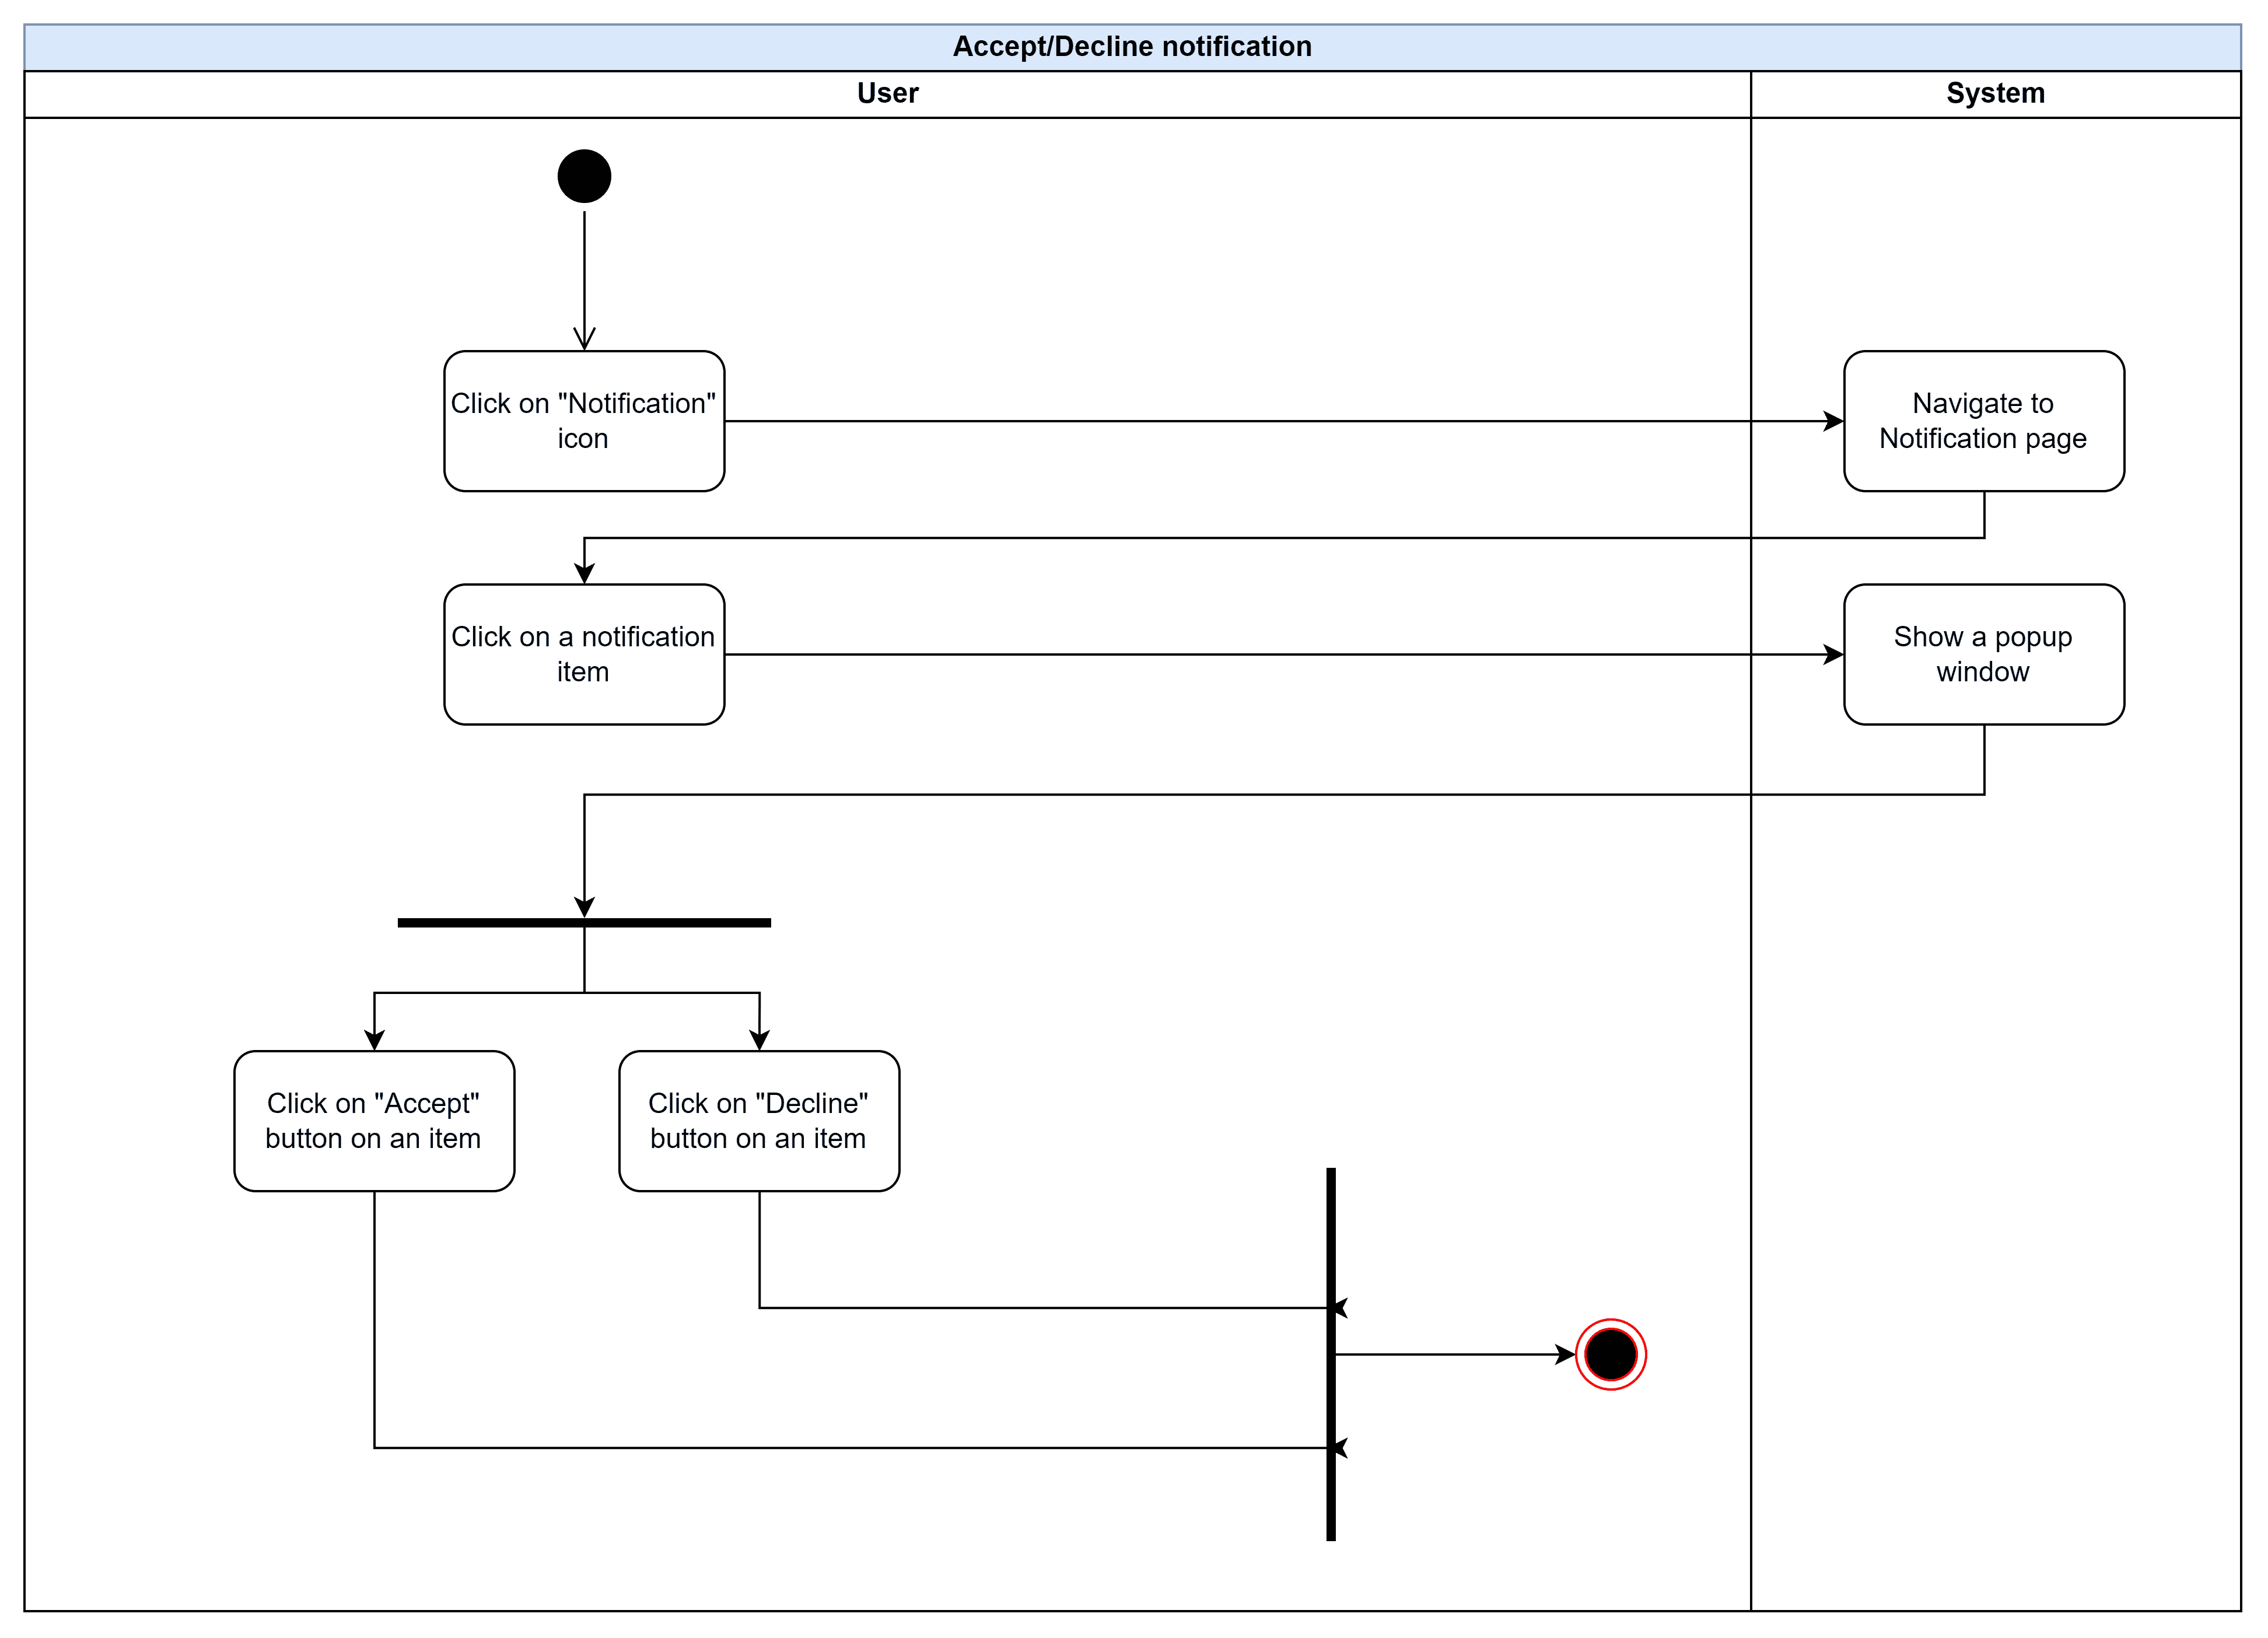
\includegraphics[width=\linewidth]{Content/Phân tích và thiết kế hệ thống/documents/Sơ đồ hoạt động/images/acceptDeclineNotification.png}
    \vspace{0.5cm}
    \caption{Chấp nhận/Từ chối lời mời tham gia Workspace}
    \label{fig:Chấp nhận/Từ chối lời mời tham gia Workspace}
\end{figure}

% Process portfolio

\newpage
\subsection{Chỉnh sửa giá trị của process version}
\begin{figure}[H]
    \centering
    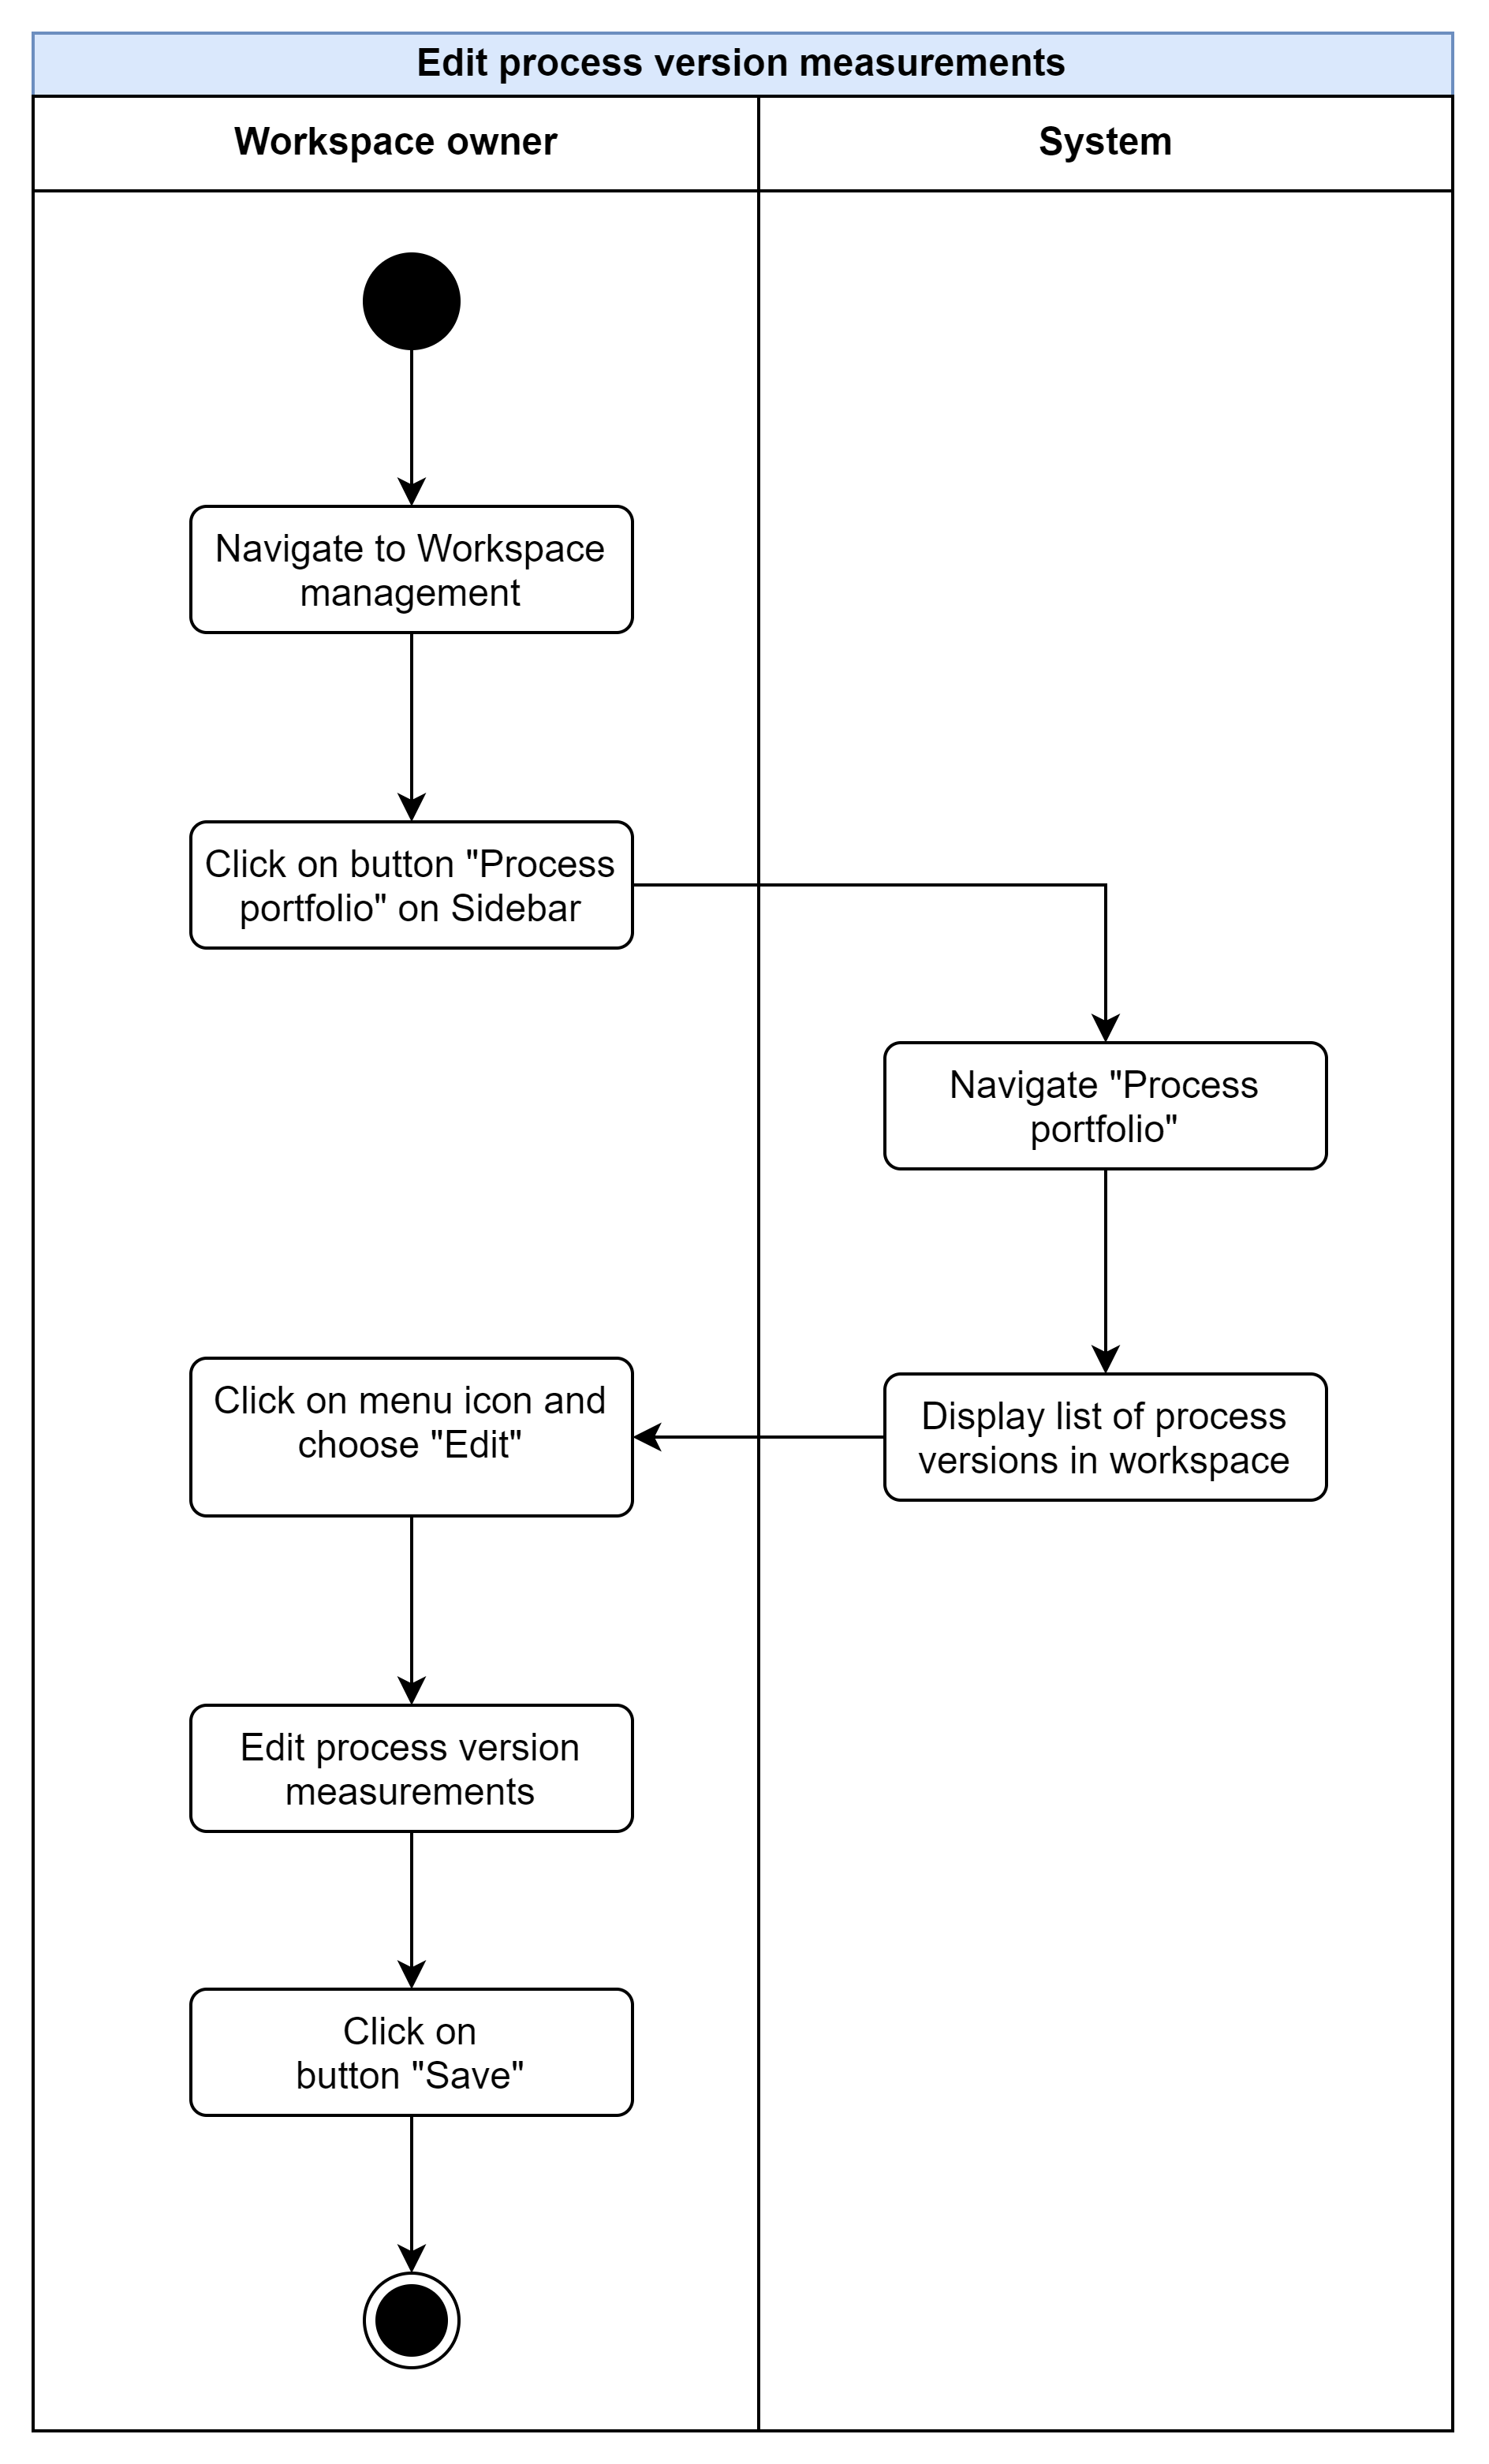
\includegraphics[width=0.8\linewidth]{Content/Phân tích và thiết kế hệ thống/documents/Sơ đồ hoạt động/images/editProcessVersionMeasurements.png}
    \vspace{0.5cm}
    \caption{Chỉnh sửa giá trị của process version}
    \label{fig:Chỉnh sửa giá trị của process version}
\end{figure}

\newpage
\subsection{Chỉnh sửa thông tin đo lường của workspace}
\begin{figure}[H]
    \centering
    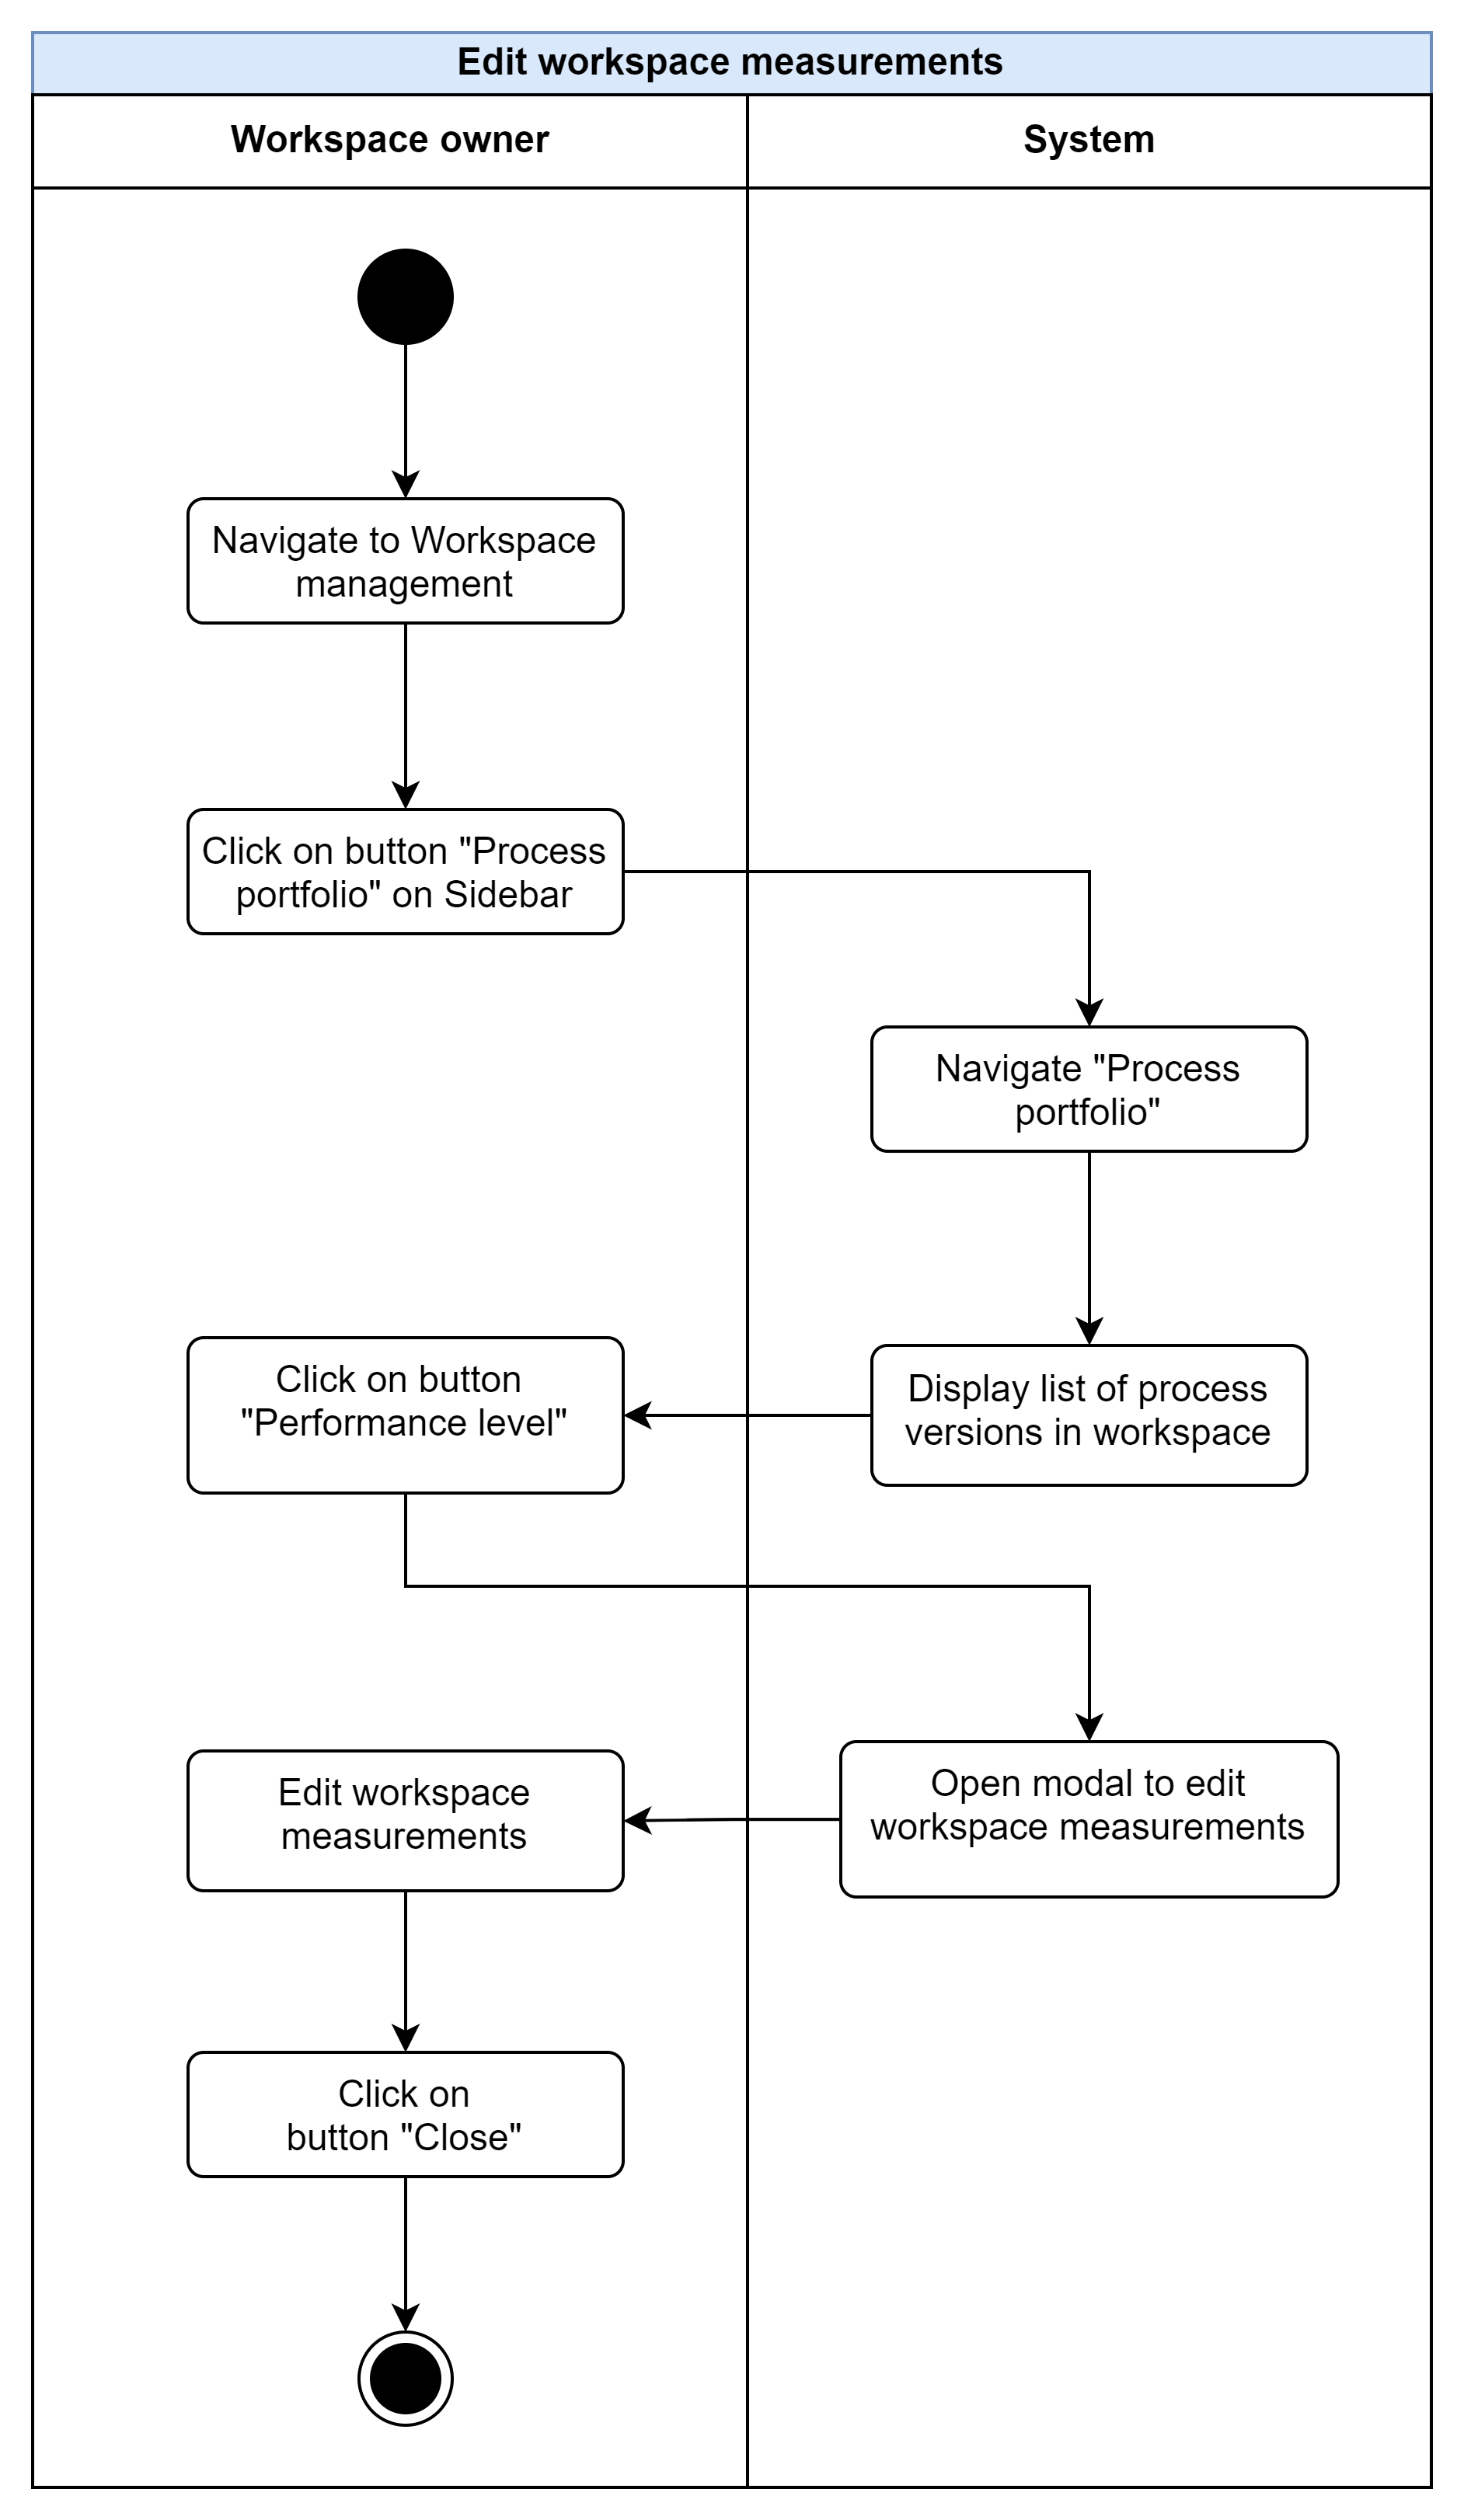
\includegraphics[width=0.8\linewidth]{Content/Phân tích và thiết kế hệ thống/documents/Sơ đồ hoạt động/images/editWorkspaceMeasurements.png}
    \vspace{0.5cm}
    \caption{Chỉnh sửa thông tin đo lường của workspace}
    \label{fig:Chỉnh sửa thông tin đo lường của workspace}
\end{figure}

\newpage
\subsection{Khởi tạo process portfolio}
\begin{figure}[H]
    \centering
    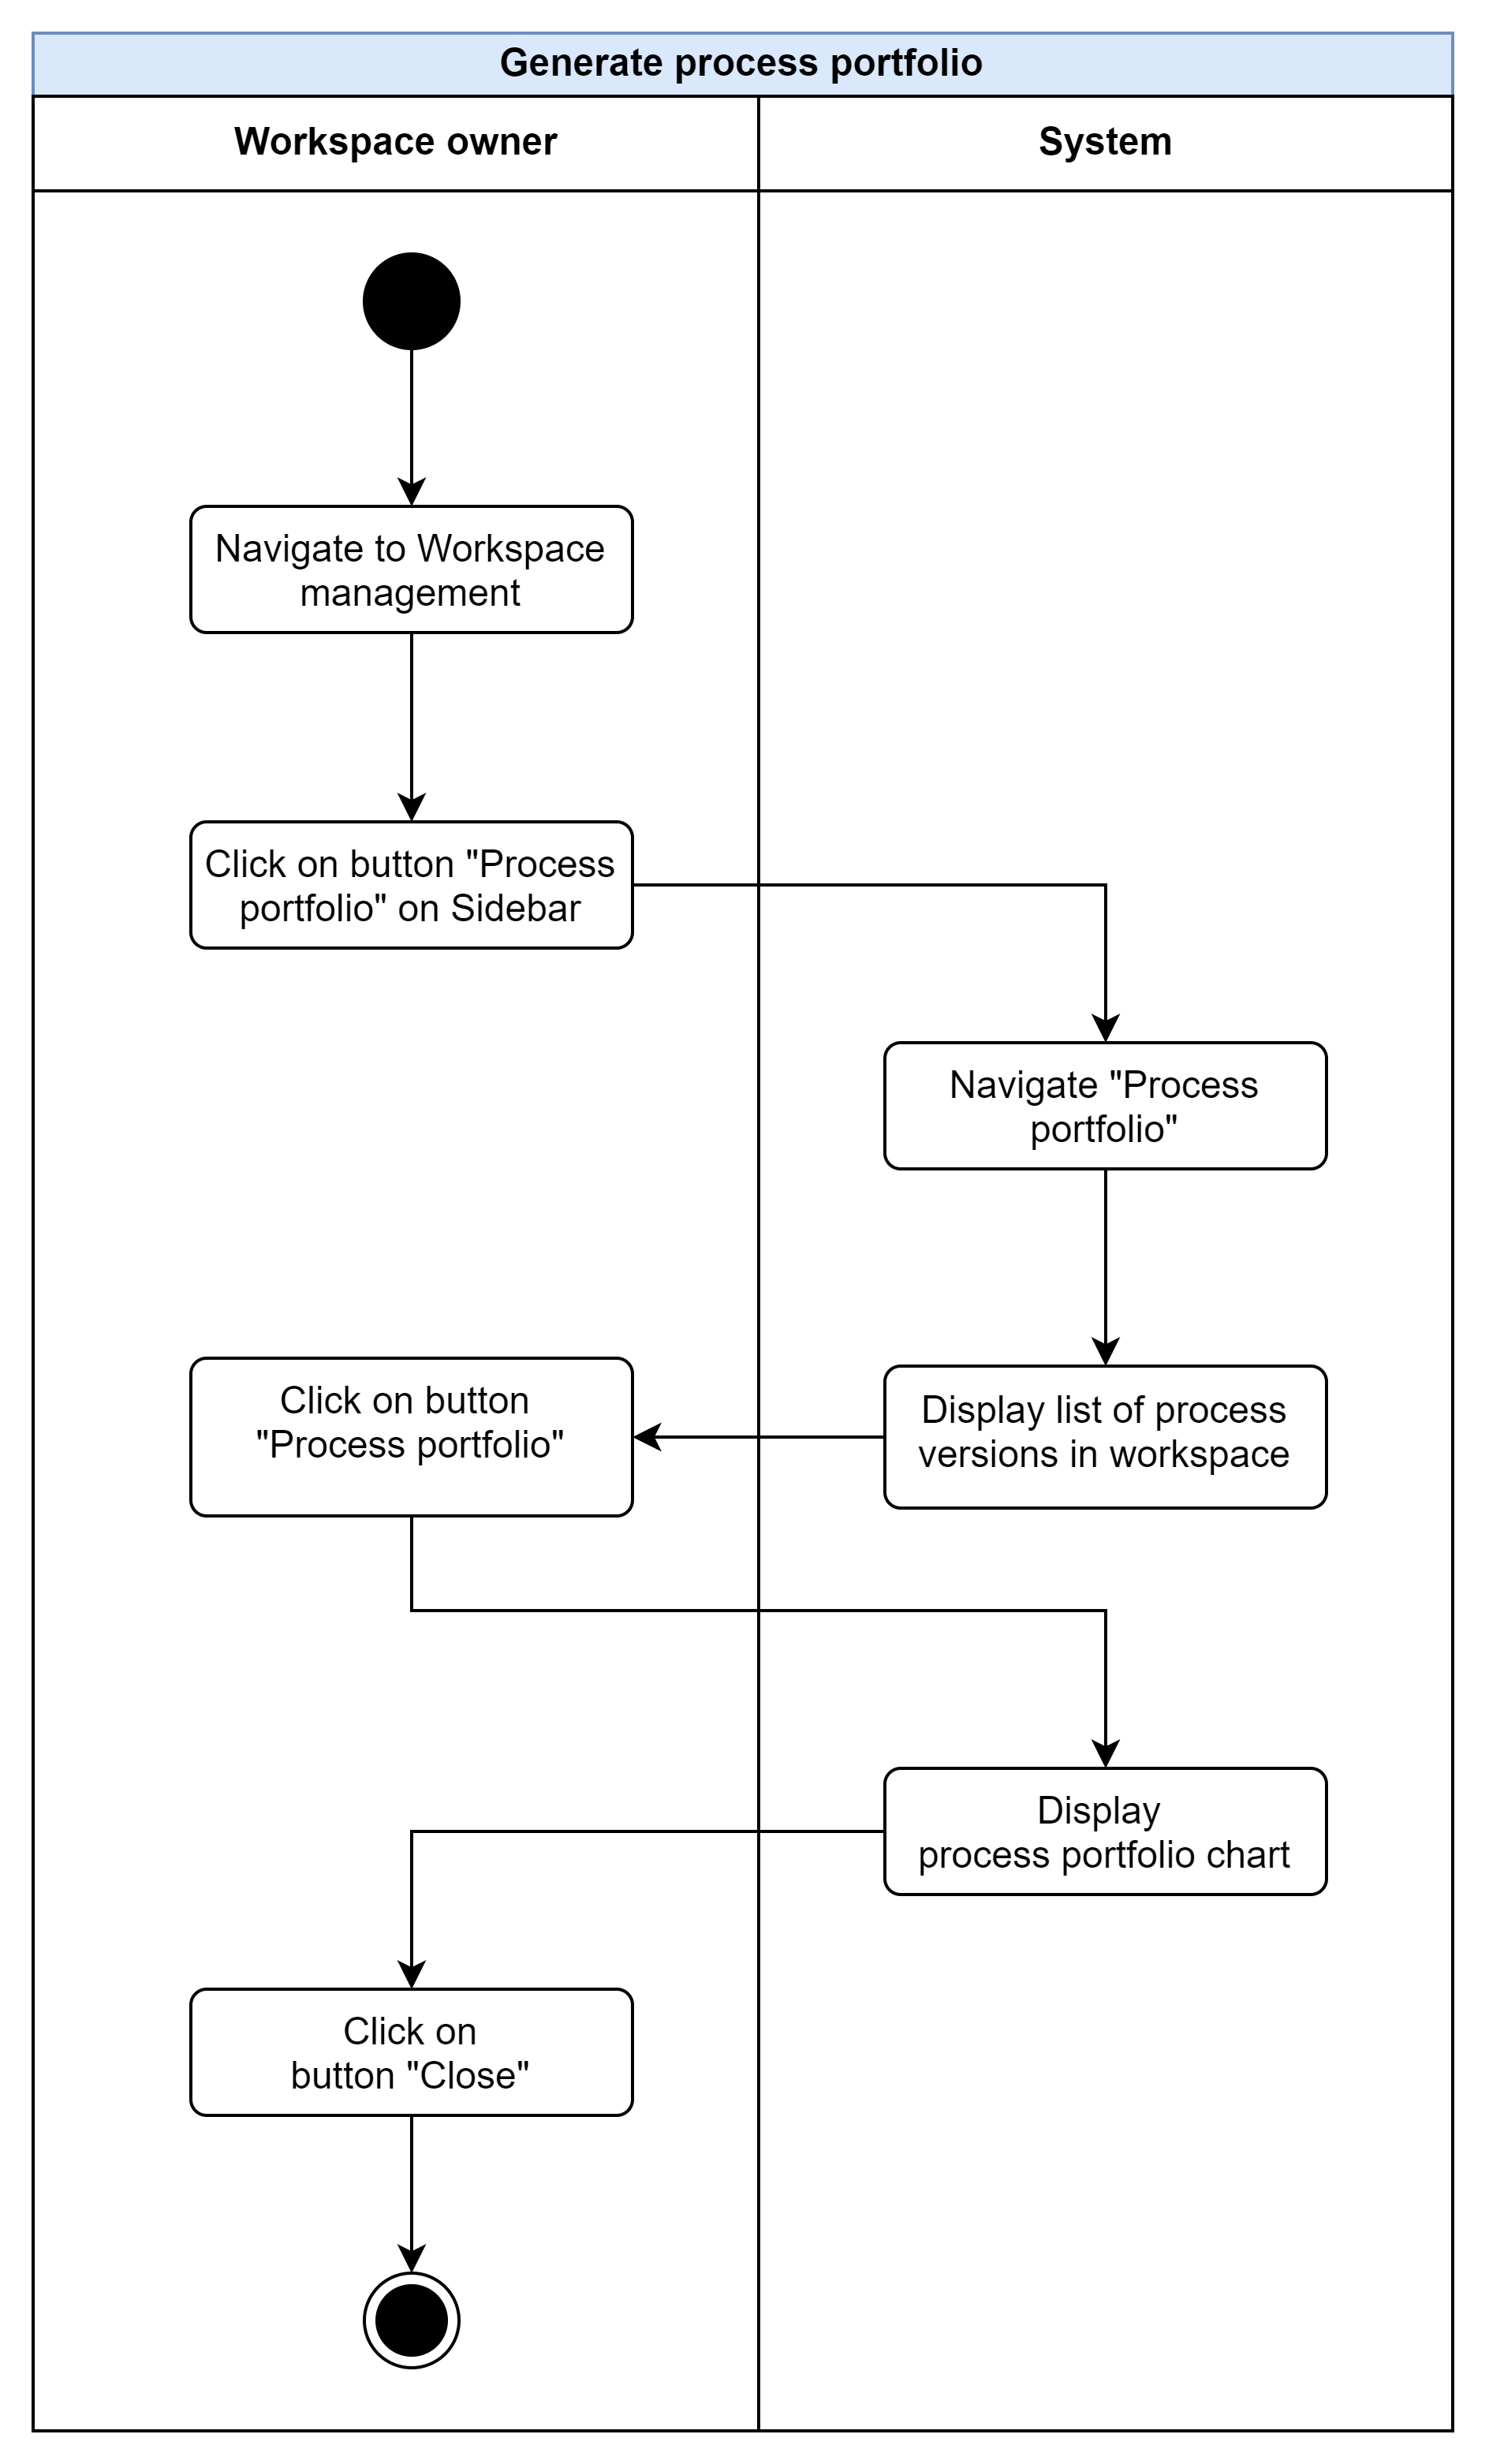
\includegraphics[width=0.8\linewidth]{Content/Phân tích và thiết kế hệ thống/documents/Sơ đồ hoạt động/images/generateProcessPortfolio.png}
    \vspace{0.5cm}
    \caption{Khởi tạo process portfolio}
    \label{fig:Khởi tạo process portfolio}
\end{figure}

\newpage
\subsection{Tạo câu hỏi trong bảng khảo sát}
\begin{figure}[H]
    \centering
    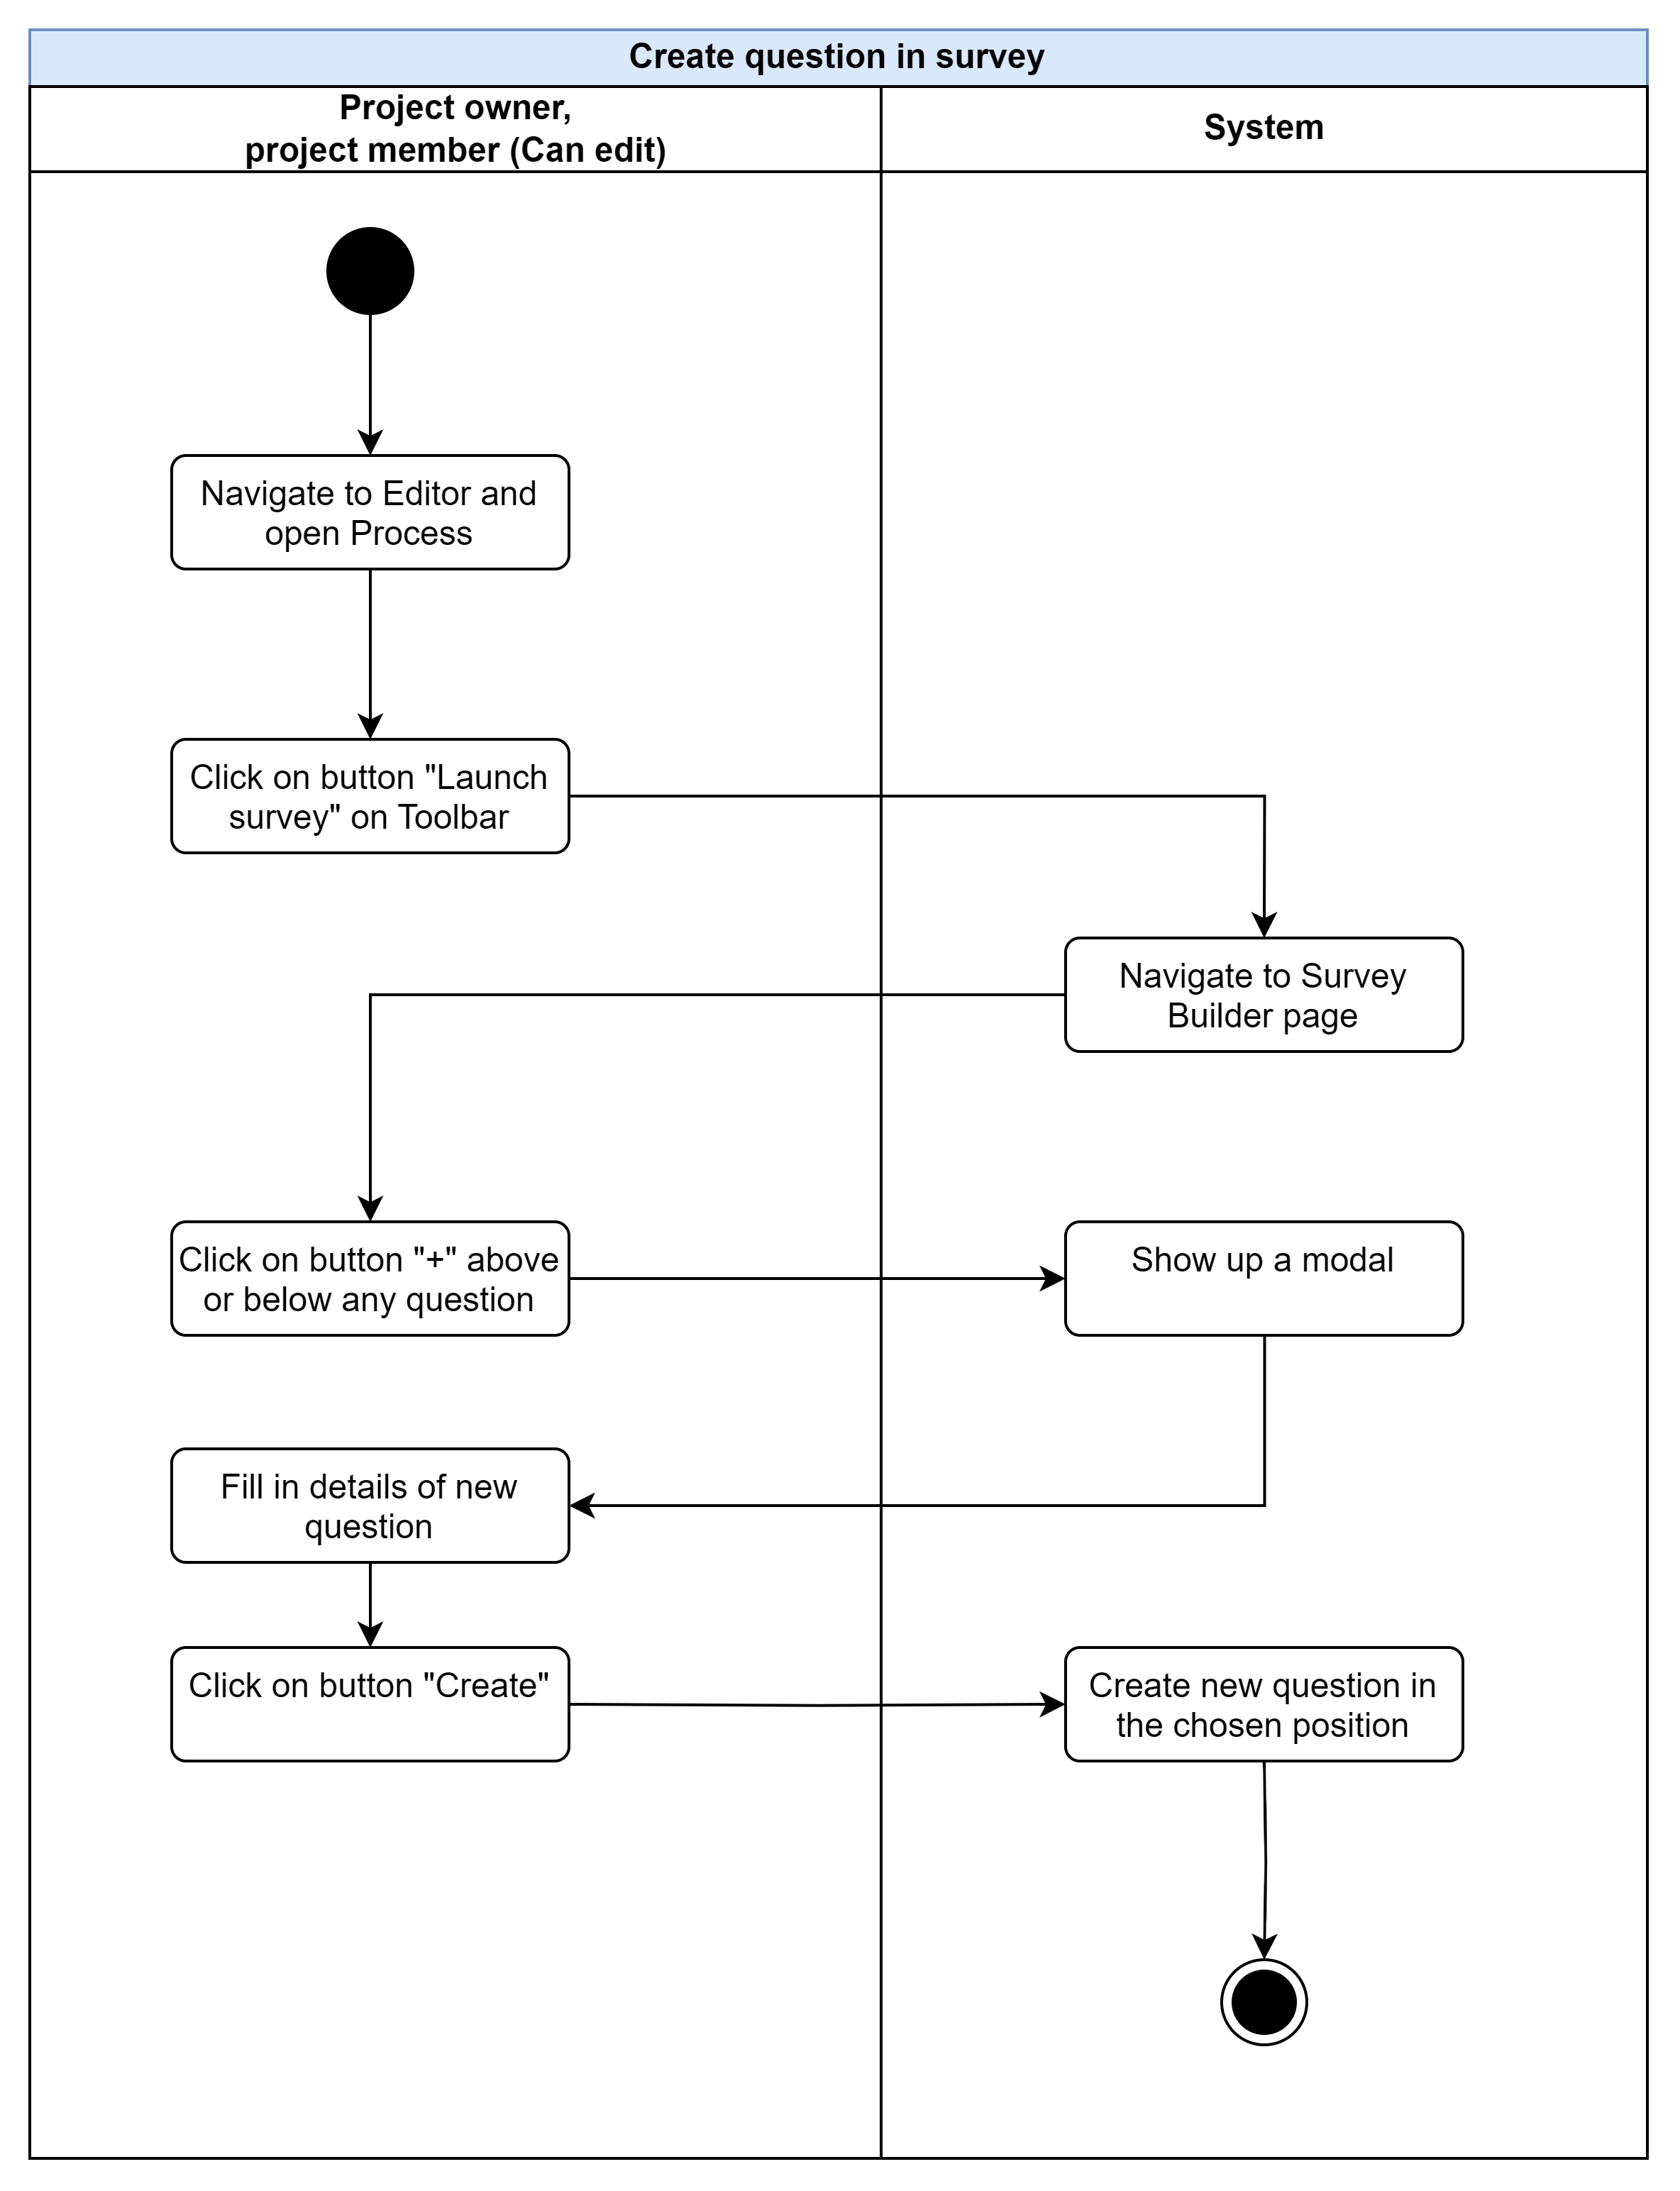
\includegraphics[width=0.8\linewidth]{Content/Phân tích và thiết kế hệ thống/documents/Sơ đồ hoạt động/images/createQuestionInSurvey.png}
    \vspace{0.5cm}
    \caption{Tạo câu hỏi trong bảng khảo sát}
    \label{fig:Tạo câu hỏi trong bảng khảo sát}
\end{figure}

\newpage
\subsection{Xoá câu hỏi trong bảng khảo sát}
\begin{figure}[H]
    \centering
    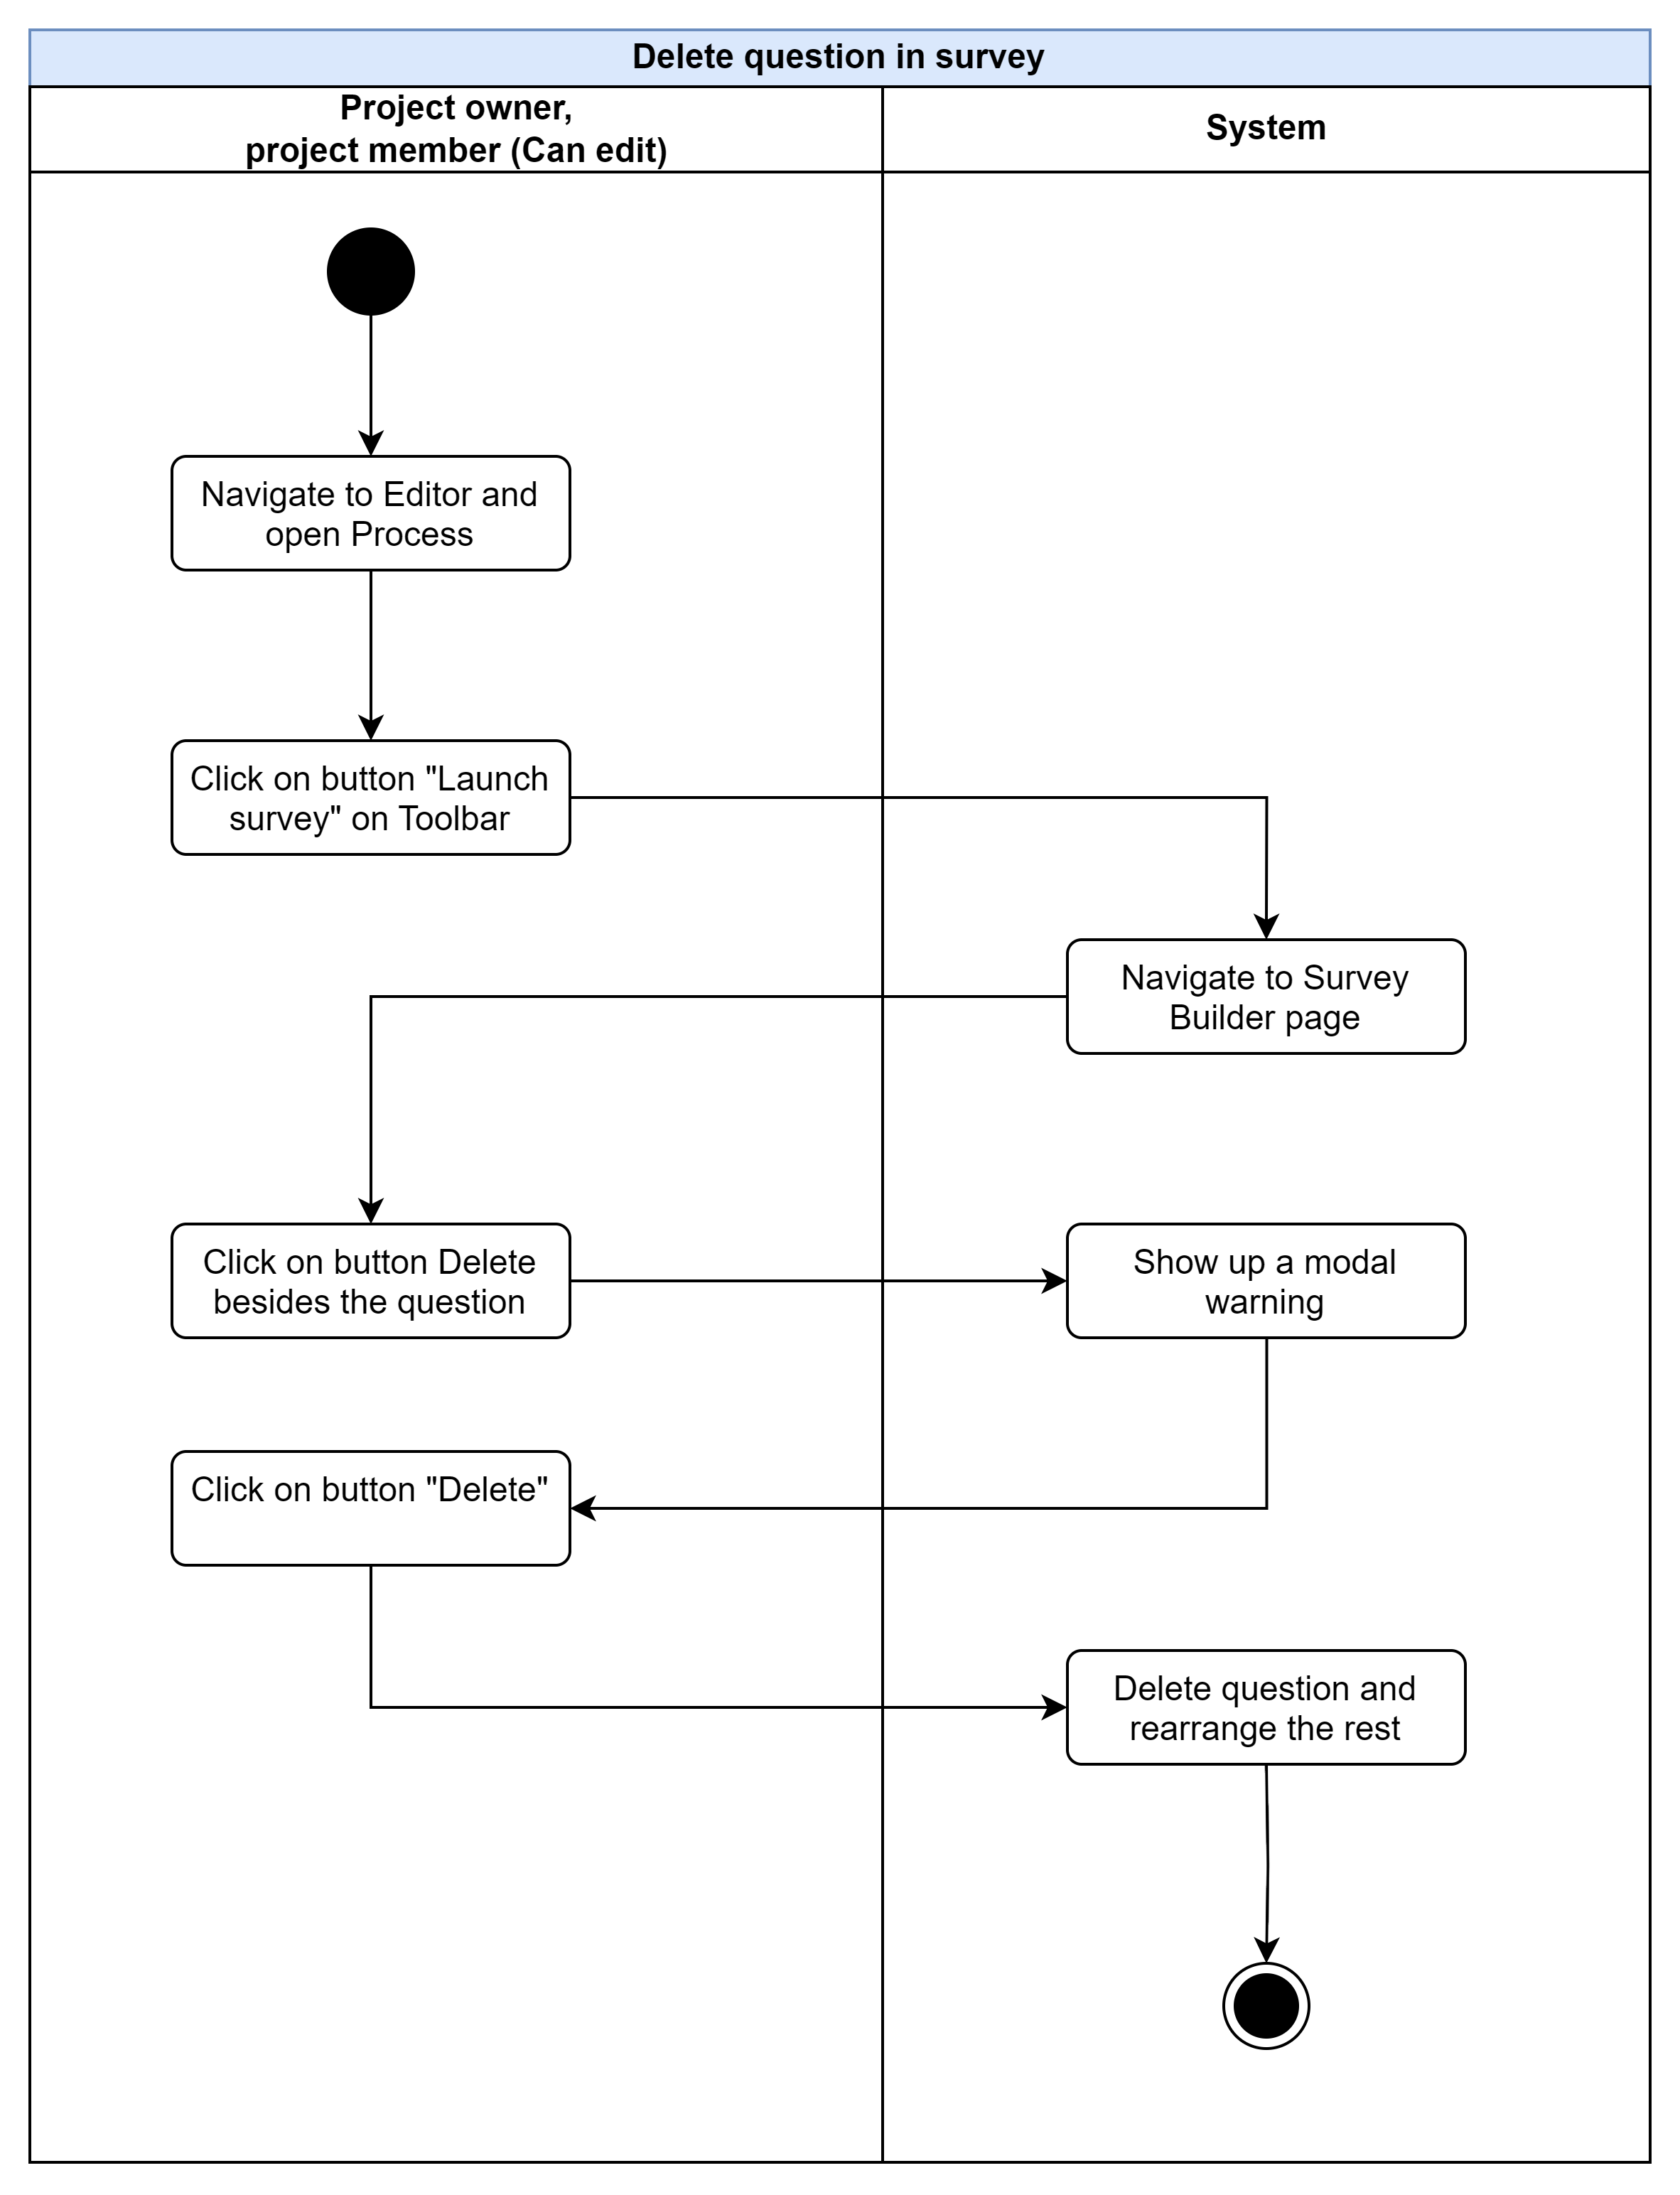
\includegraphics[width=0.8\linewidth]{Content/Phân tích và thiết kế hệ thống/documents/Sơ đồ hoạt động/images/deleteQuestionInSurvey.png}
    \vspace{0.5cm}
    \caption{Xoá câu hỏi trong bảng khảo sát}
    \label{fig:Xoá câu hỏi trong bảng khảo sát}
\end{figure}

\newpage
\subsection{Kéo thả câu hỏi đến vị trí mới trong bảng khảo sát}
\begin{figure}[H]
    \centering
    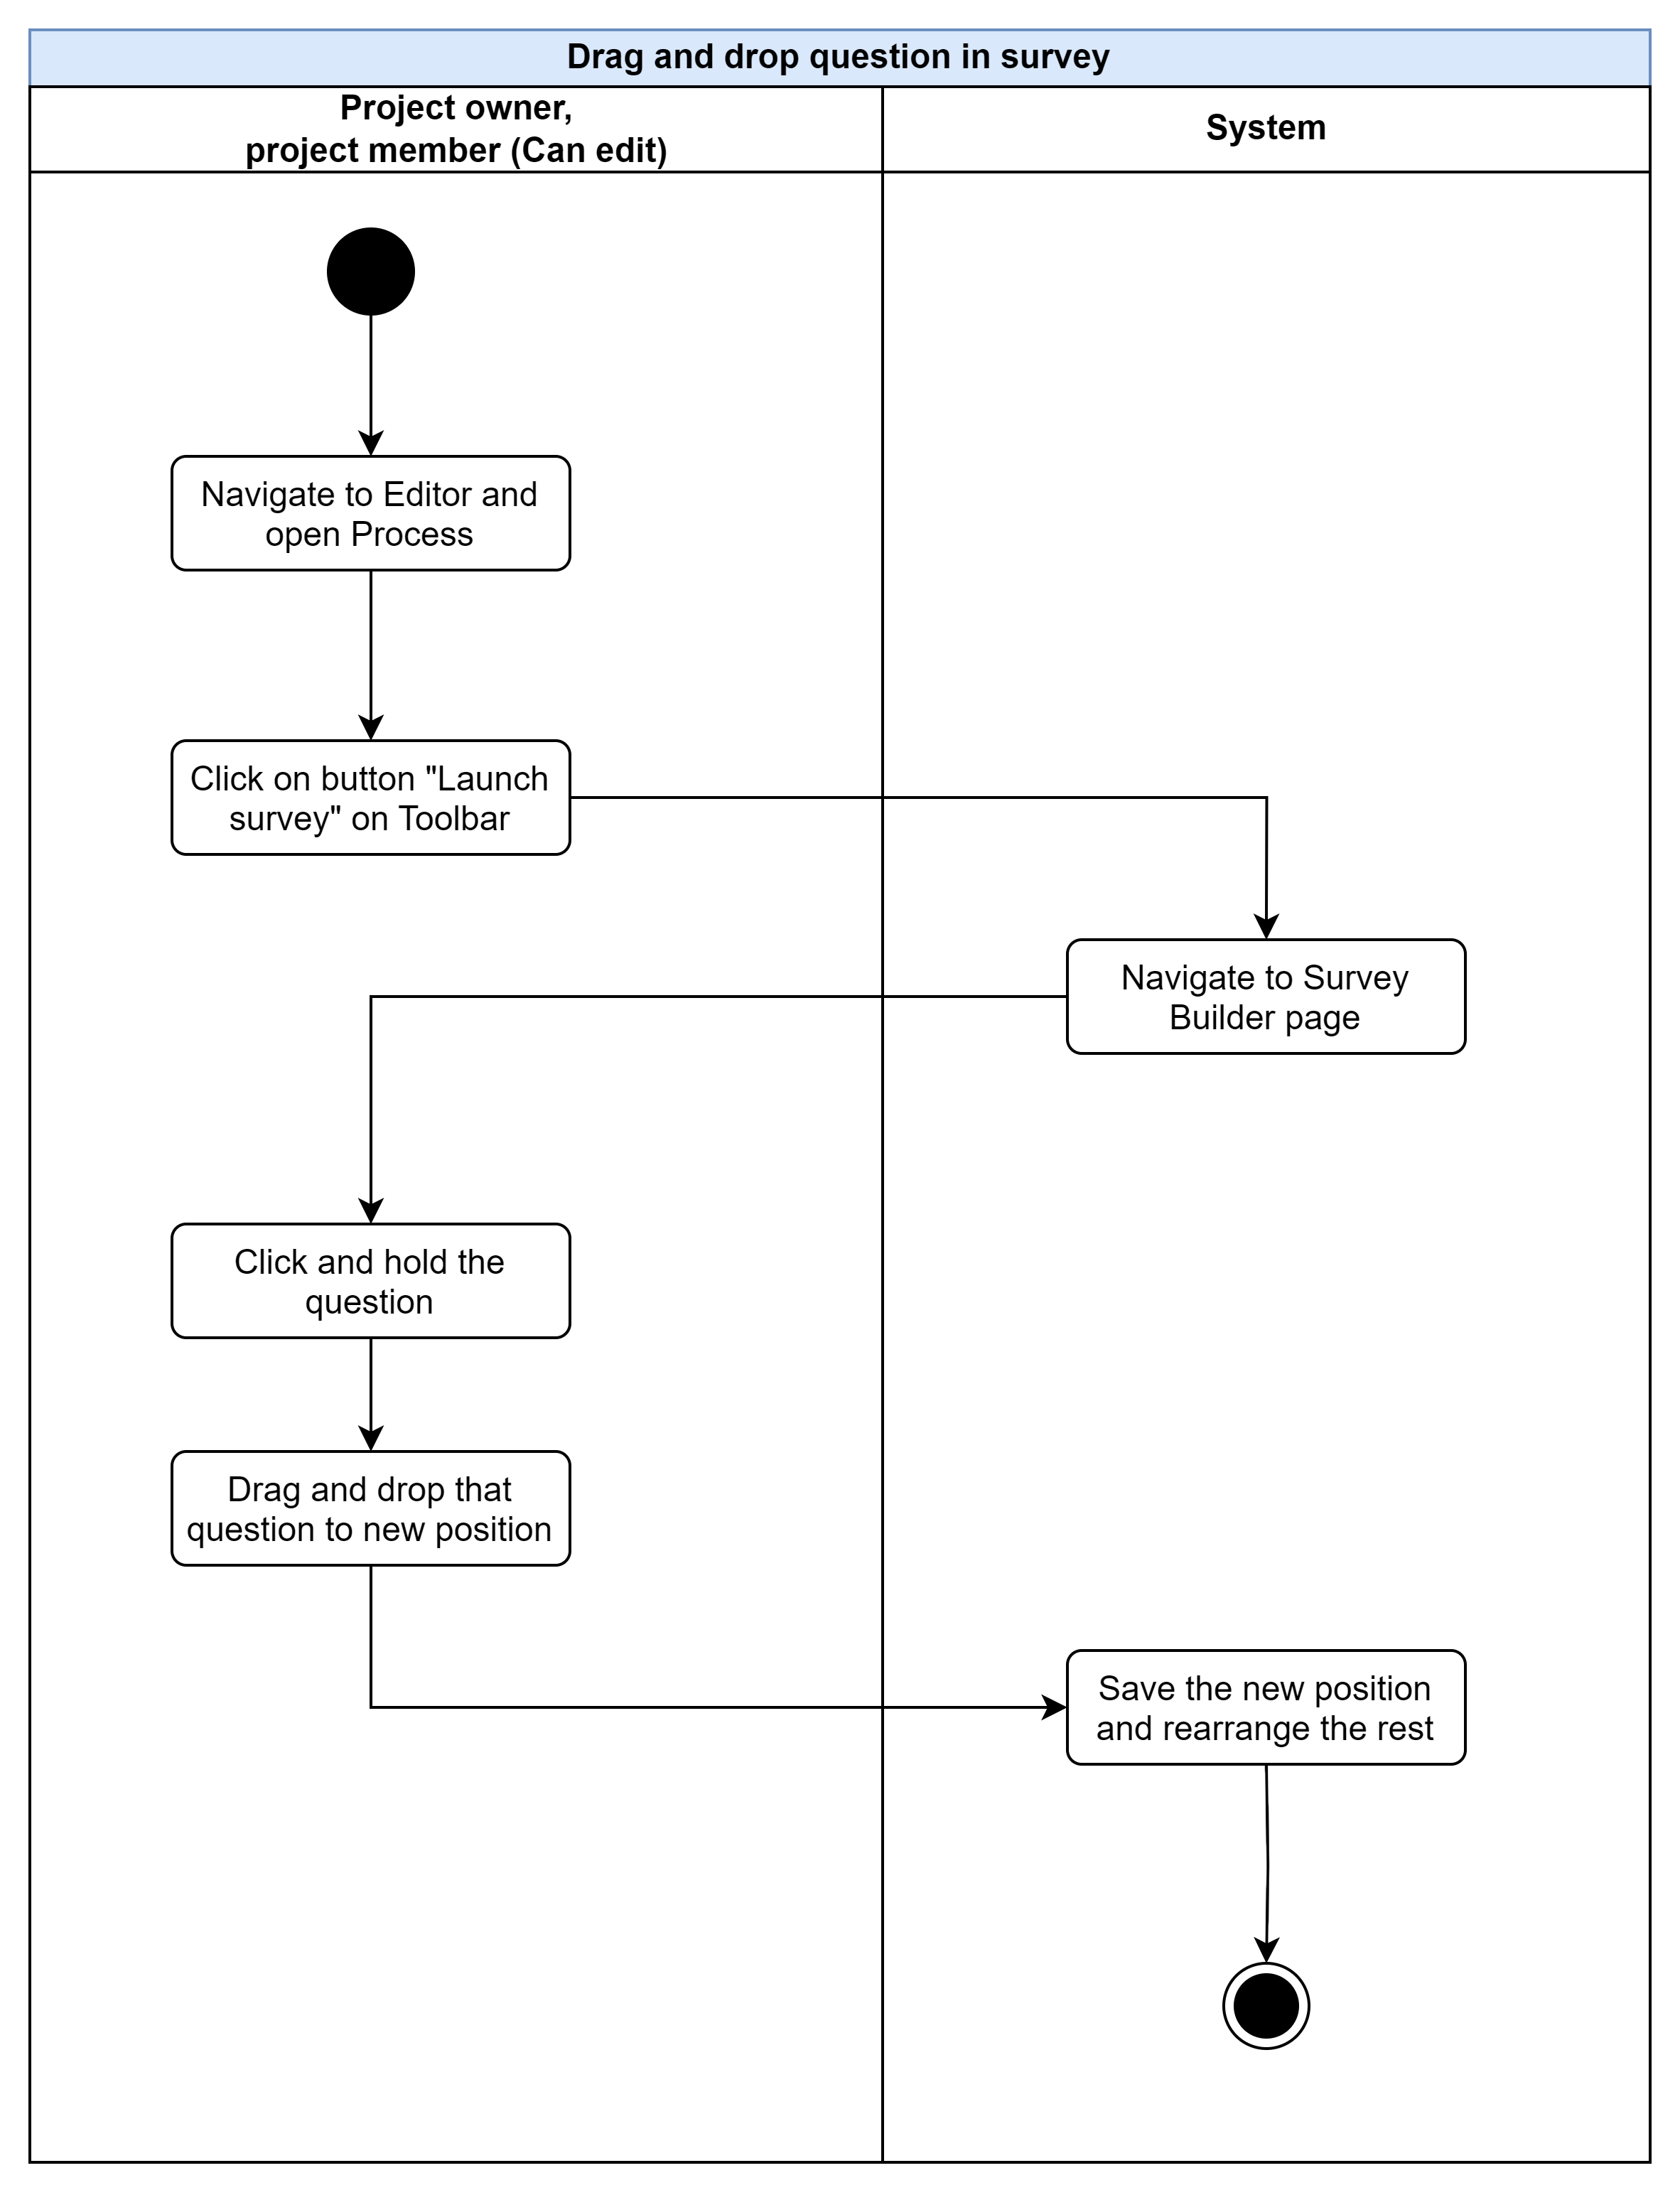
\includegraphics[width=0.8\linewidth]{Content/Phân tích và thiết kế hệ thống/documents/Sơ đồ hoạt động/images/dragAnDropQuestionInSurvey.png}
    \vspace{0.5cm}
    \caption{Kéo thả câu hỏi đến vị trí mới trong bảng khảo sát}
    \label{fig:Kéo thả câu hỏi đến vị trí mới trong bảng khảo sát}
\end{figure}

\newpage
\subsection{Công bố bảng khảo sát}
\begin{figure}[H]
    \centering
    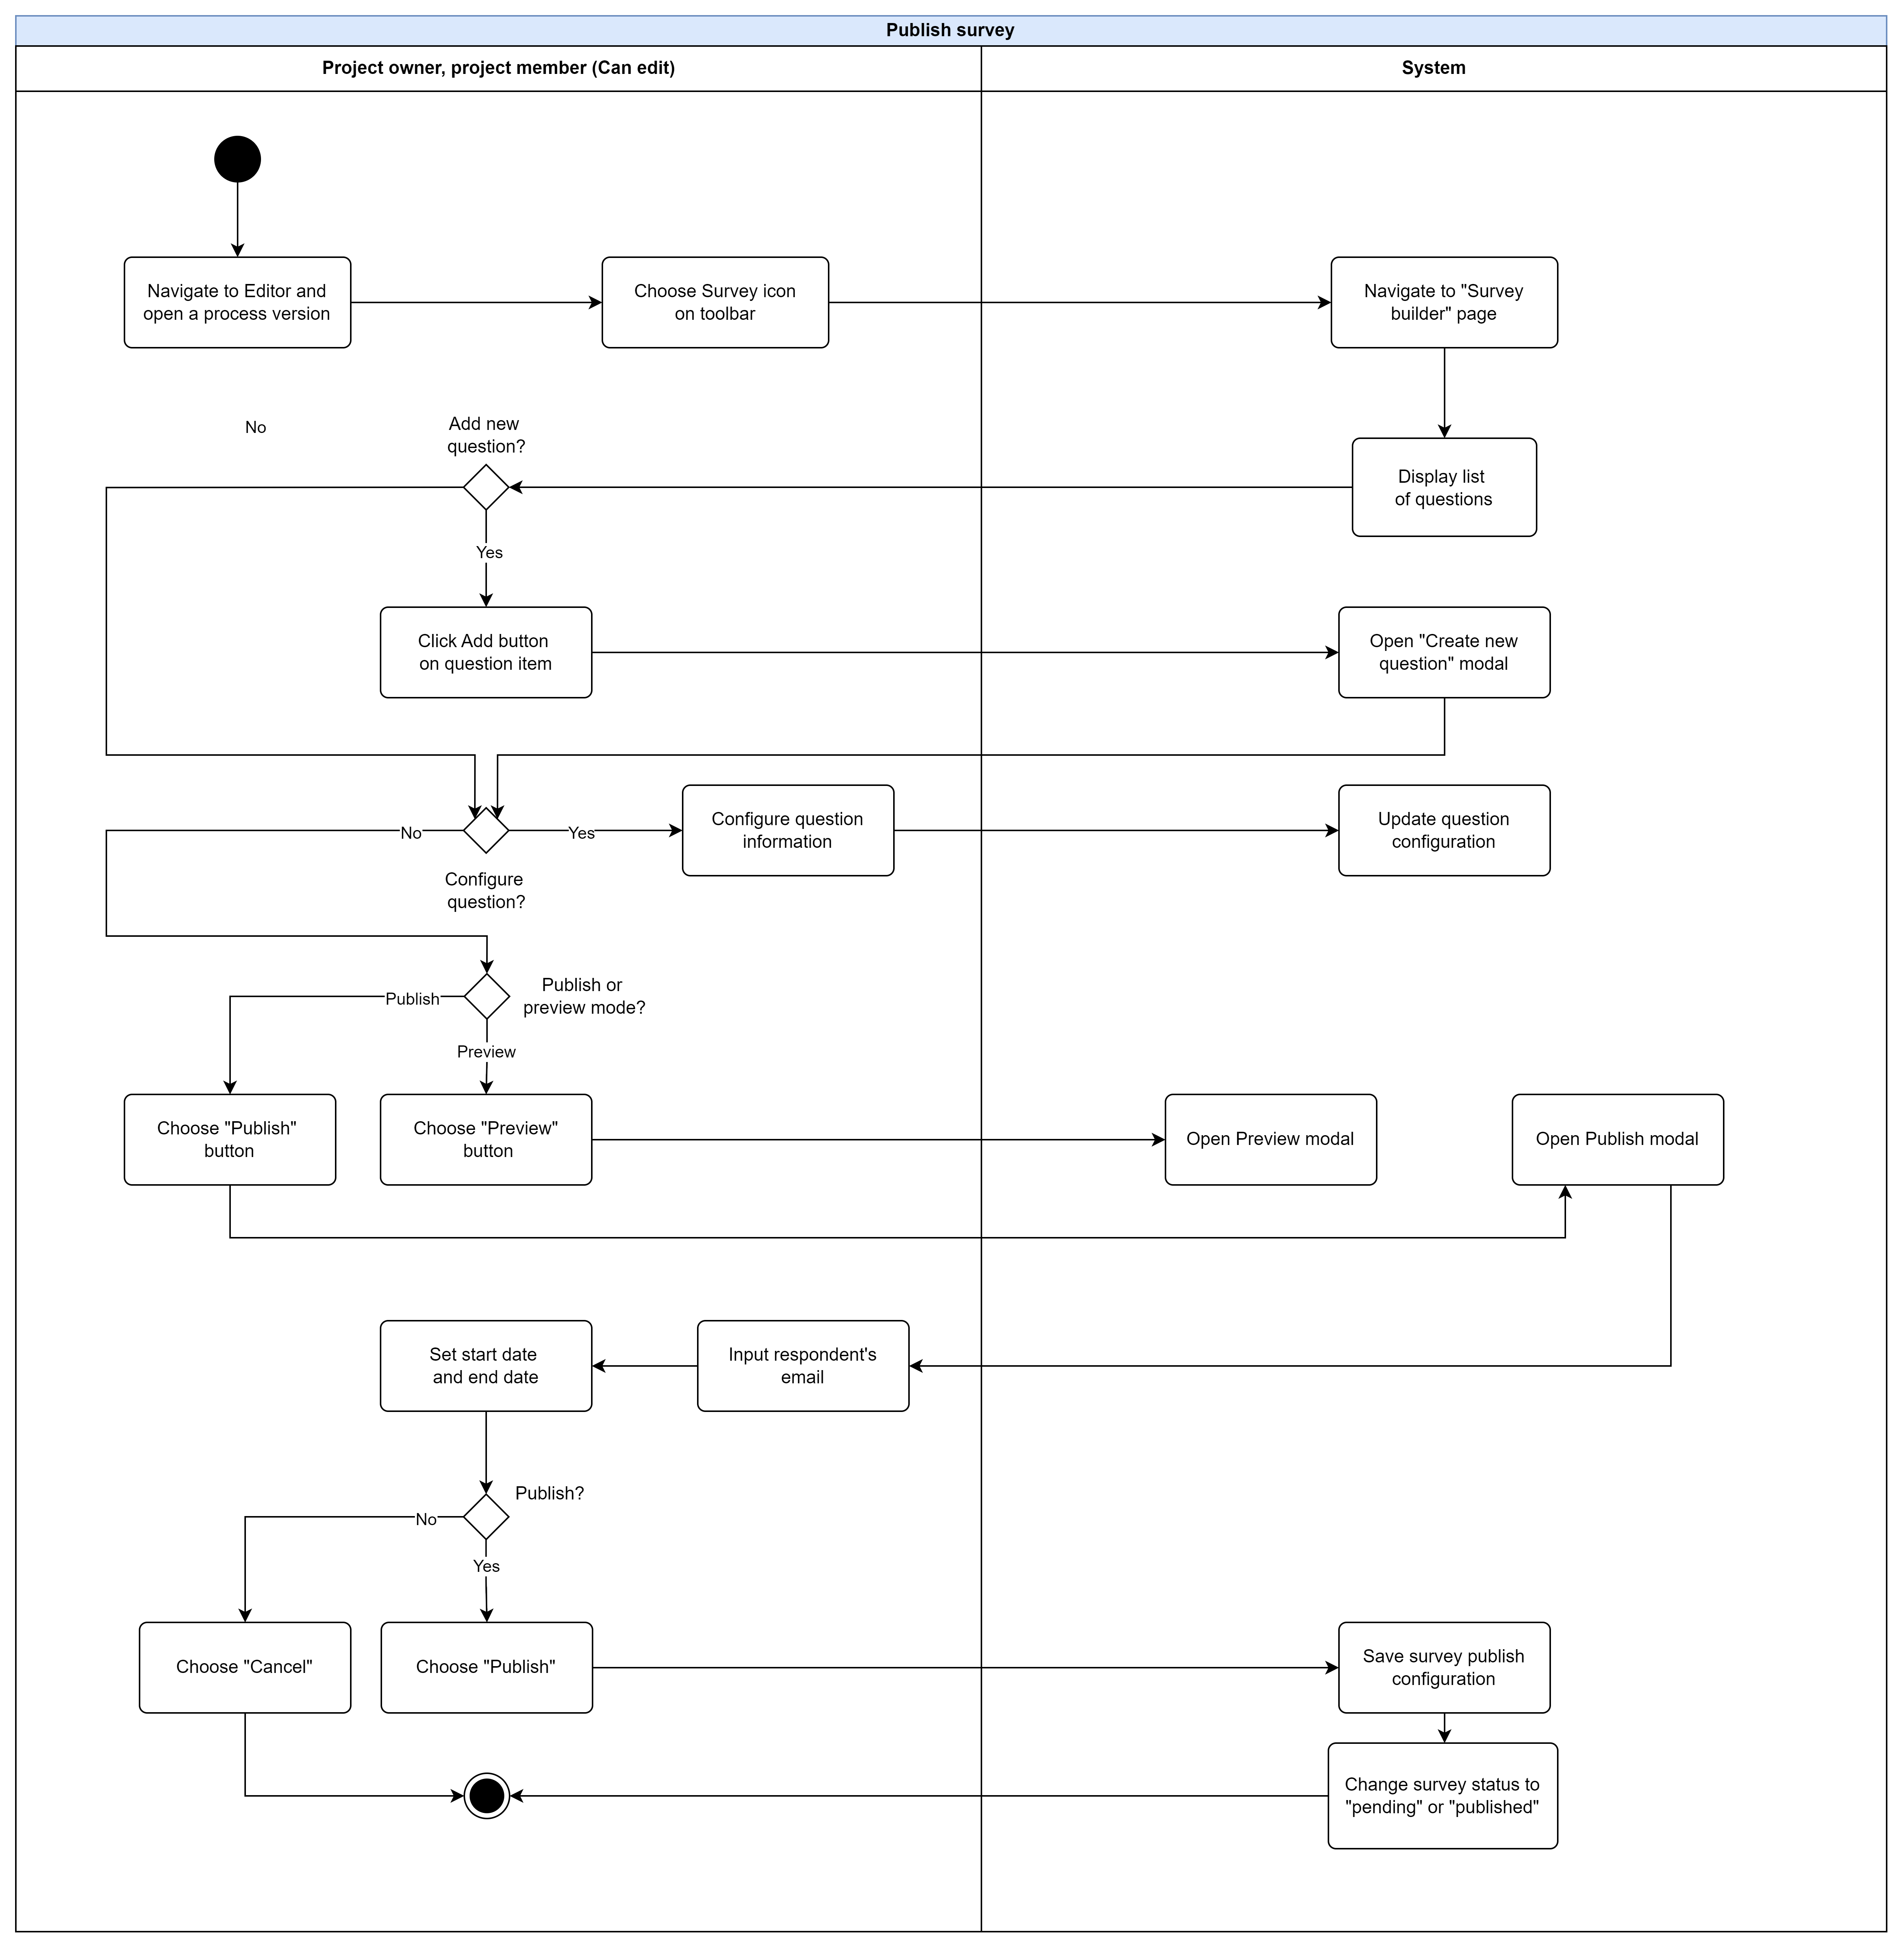
\includegraphics[width=0.8\linewidth]{Content/Phân tích và thiết kế hệ thống/documents/Sơ đồ hoạt động/images/publishSurvey.png}
    \vspace{0.5cm}
    \caption{Công bố bảng khảo sát}
    \label{fig:Công bố bảng khảo sát}
\end{figure}
\section{Sơ đồ lớp}

% \subsubsection{Tổng quan}
\begin{figure}[H]
    \centering
    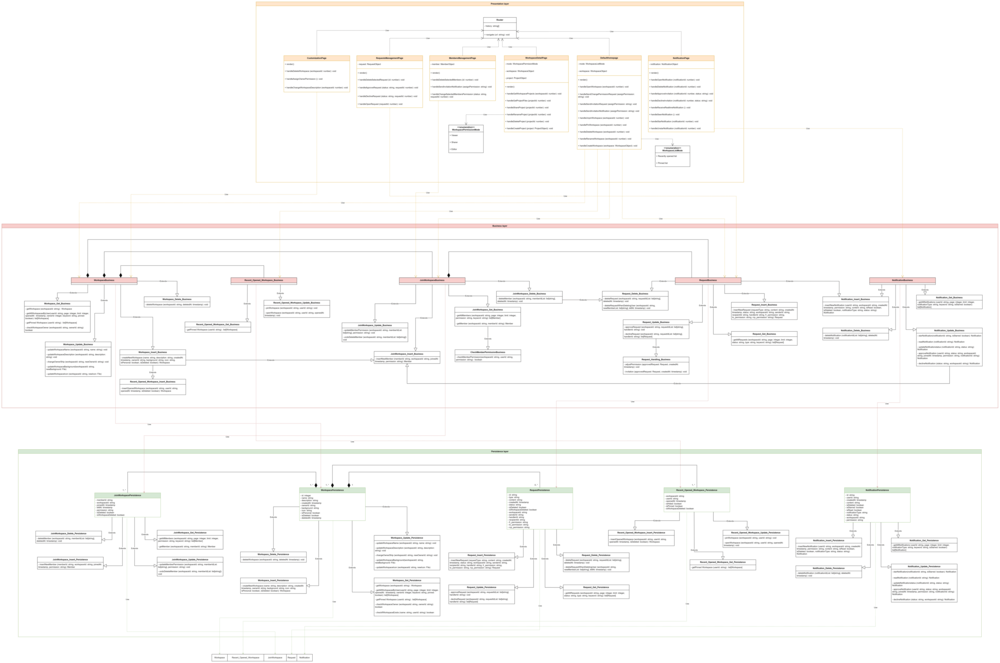
\includegraphics[width=\linewidth]{Content/Phân tích và thiết kế hệ thống/documents/Sơ đồ lớp/images/LayerArchitect.png}
    \vspace{0.5cm}
    \caption{Sơ đồ lớp cho toàn bộ hệ thống}
    \label{fig:Sơ đồ lớp cho toàn bộ hệ thống}
\end{figure}

\par
Do một số hạn chế về không gian, chúng tôi không thể trình bày toàn bộ sơ đồ lớp,
vì vậy chúng tôi xin cung cấp đường link dẫn đến sơ đồ lớp chi tiết như sau:
\url{https://drive.google.com/file/d/1Wh5EIWwnRwMF--LBoFeL5nTtOkbEX_9S/view?usp=sharing}

\subsection{Presentation Layer}
\begin{figure}[H]
    \centering
    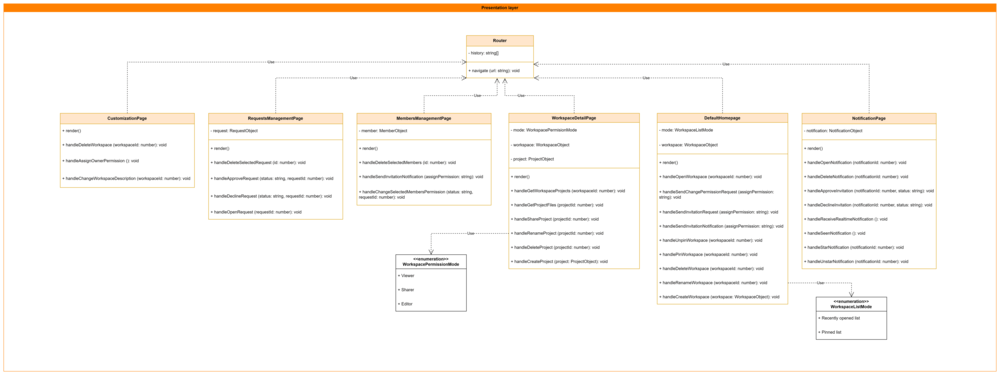
\includegraphics[ width = \linewidth]{Content/Phân tích và thiết kế hệ thống/documents/Sơ đồ lớp/images/Presentation layer/presentationLayer.png}
    \vspace{0.5cm}
    \caption{Tổng quan Presentation Layer}
    \label{fig:Tổng quan Presentation layer}
\end{figure}
Tầng presentation biểu diễn những giao diện được hiện thực, nó sẽ bao gồm cả những trạng thái (mode) của giao diện cũng như những hàm hiện thực chức năng logic của giao diện tương ứng.
Chi tiết cụ thể hơn sẽ được trình bày trong phần dưới theo từng class được hiện thực.

\begin{figure}[H]
    \centering
    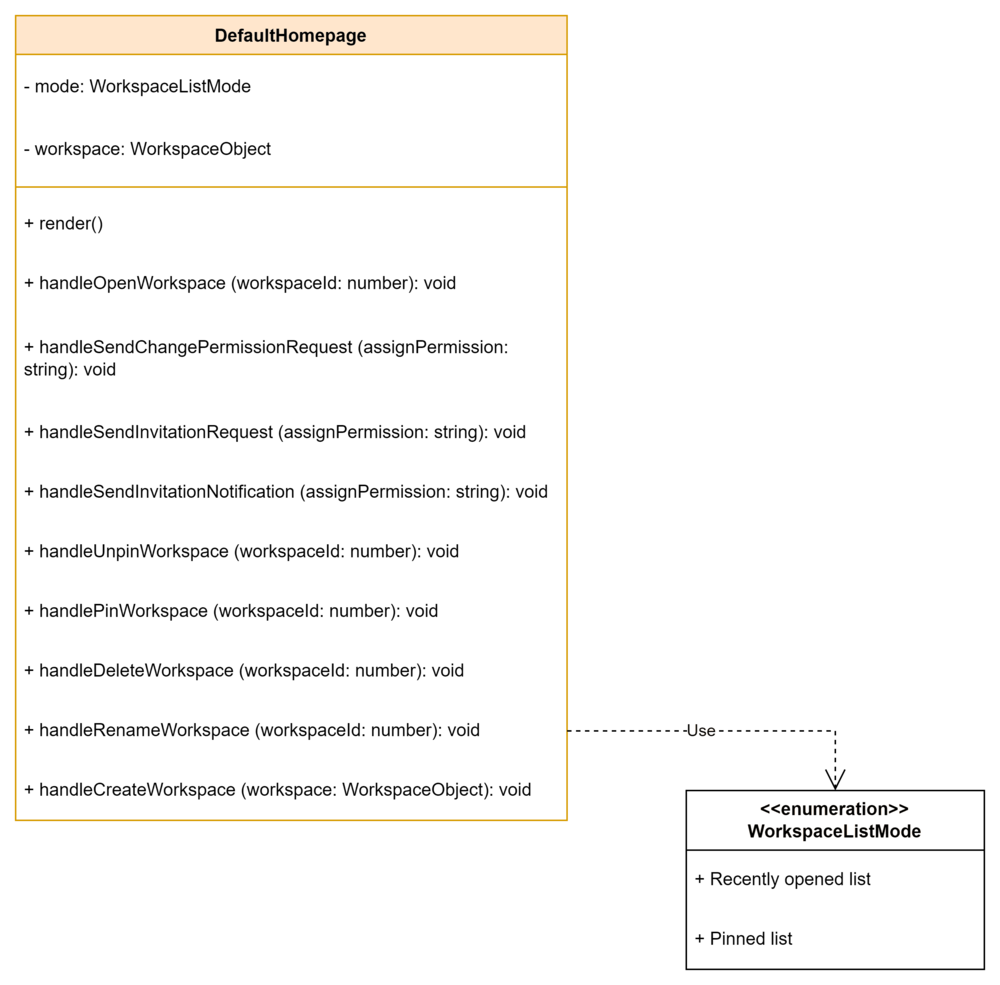
\includegraphics[ width = 0.7\linewidth]{Content/Phân tích và thiết kế hệ thống/documents/Sơ đồ lớp/images/Presentation layer/defaultWorkspacePage.png}
    \vspace{0.5cm}
    \caption{Class DefaultHomepage trong Presentation layer}
    \label{fig:Class Default homepage trong Presentation layer}
\end{figure}
Ở giao diện mặc định khi người dùng được chuyển hướng tới sau khi hoàn tất thủ tục xác thực với hệ thống, chúng ta sẽ tập trung vào những chức năng liên quan tới việc hiển thị và tương tác với workspace mà người dùng tham gia (create, open, pin, delete, rename). Những chức năng đáng chú ý là nhóm chức năng gửi lời mời vào workspace/gửi yêu cầu mời người dùng khác vào workspace, nhóm chức năng này được xử lý real-time (thời gian thực) để nhận và hiển thị dữ liệu ở những giao diện khác. Giao diện sẽ có hai hình thức hiển thị danh sách workspace là theo thời gian mở workspace gần nhất - "Recently opened workspace" và những workspace được người dùng ghim thủ công - "Pinned workspace".

\begin{figure}[H]
    \centering
    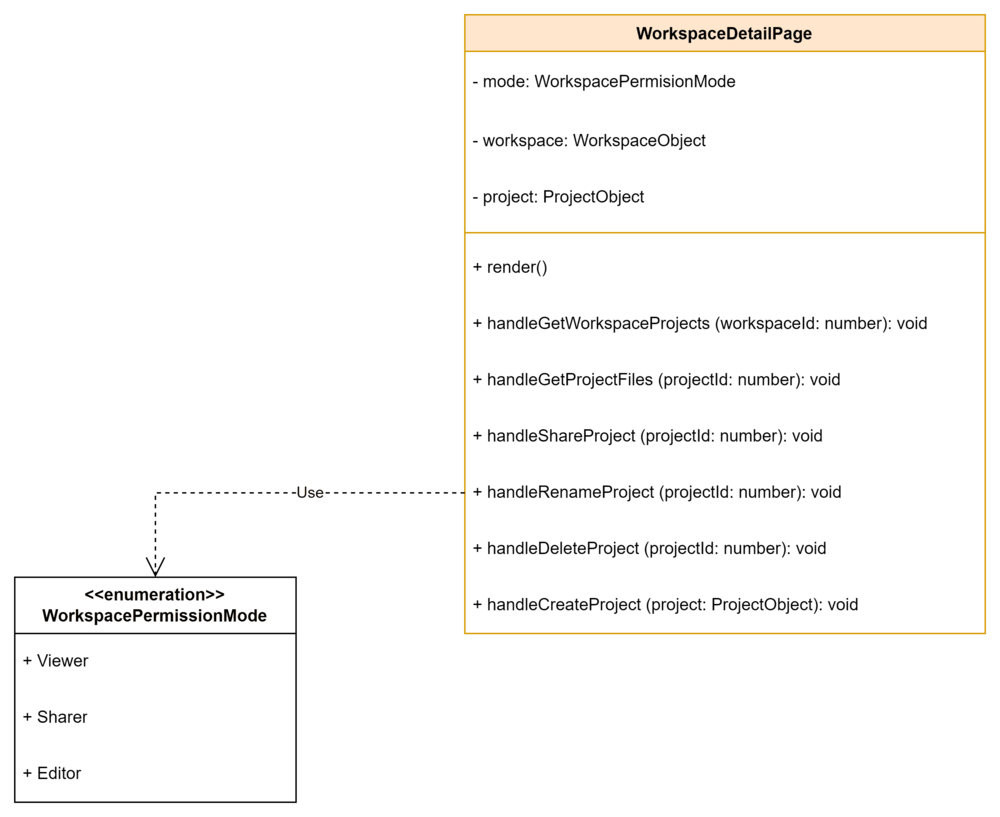
\includegraphics[ width = 0.7\linewidth]{Content/Phân tích và thiết kế hệ thống/documents/Sơ đồ lớp/images/Presentation layer/workspaceDetailPage.png}
    \vspace{0.5cm}
    \caption{Class WorkspaceDetailPage trong Presentation layer}
    \label{fig:Class WorkspaceDetailPage trong Presentation layer}
\end{figure}
Người dùng sẽ được chuyển hướng tới giao diện hiển thị nội dung bên trong workspace khi sử dụng chức năng "Open workspace" hoặc chọn item workspace tương ứng, nội dung bên trong workspace sẽ được hiển thị dưới dạng danh sách những project có bên trong workspace. Mỗi project sẽ là bao gồm nhiều process/version của process và document bên trong. Người dùng sẽ được phân quyền hạn khi tham gia vào workspace: viewer, sharer và editor.

\begin{figure}[H]
    \centering
    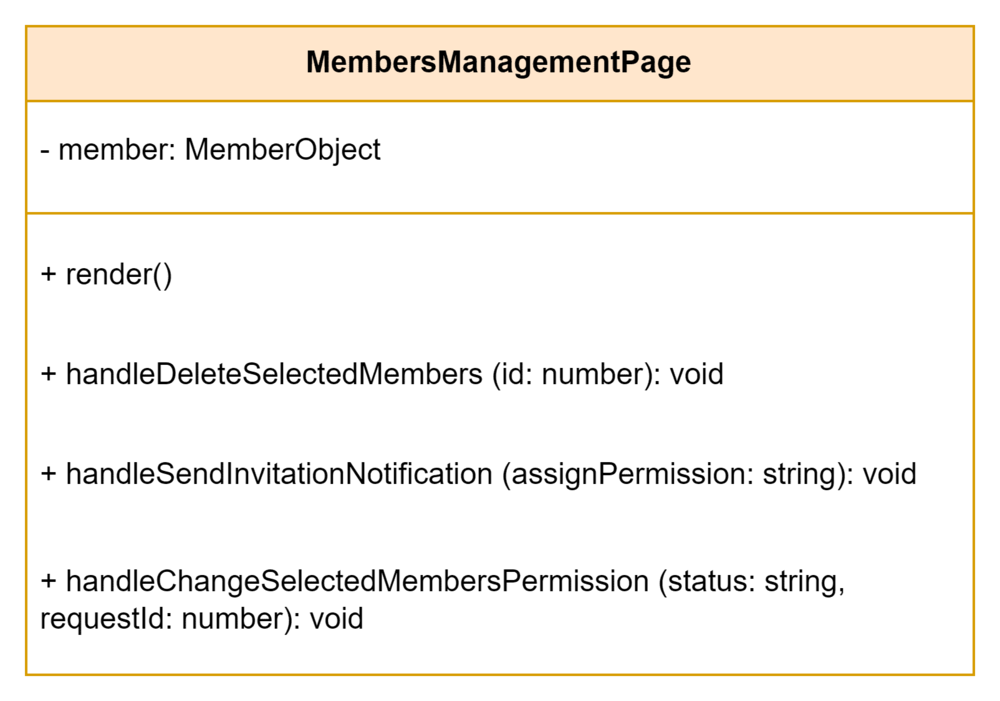
\includegraphics[ width = 0.5\linewidth]{Content/Phân tích và thiết kế hệ thống/documents/Sơ đồ lớp/images/Presentation layer/membersManagementPage.png}
    \vspace{0.5cm}
    \caption{Class MemberManagementPage trong Presentation layer}
    \label{fig:Class MemberManagementPage trong Presentation layer}
\end{figure}
Giao diện quản lý thành viên trong workspace là mục mặc định được điều hướng khi người sở hữu workspace chuyển hướng tới giao diện quản lý. Class này sẽ tập trung hiện thực những chức năng liên quan tới thêm/xóa thành viên trong workspace và điều chỉnh quyền hạn của thành viên tương ứng trong workspace. Ngoài ra còn có chức năng gửi lời mời vào workspace cho người dùng khác, chức năng này cũng sẽ được xử lý real-time để hiển thị dữ liệu ở giao diện thông báo cá nhân khi người dùng khác nhận được lời mời.

\begin{figure}[H]
    \centering
    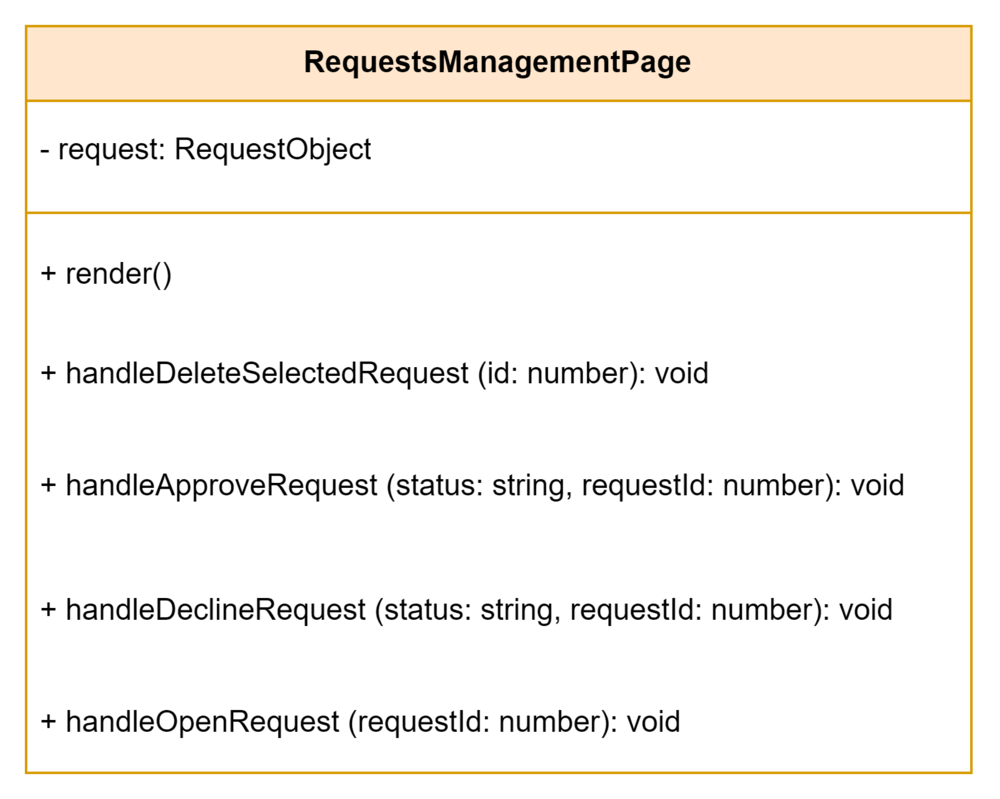
\includegraphics[ width = 0.5\linewidth]{Content/Phân tích và thiết kế hệ thống/documents/Sơ đồ lớp/images/Presentation layer/requestManagementPage.png}
    \vspace{0.5cm}
    \caption{Class RequestManagementPage trong Presentation layer}
    \label{fig:Class RequestManagementPage trong Presentation layer}
\end{figure}
Giao diện quản lý yêu cầu sẽ hiển thị những yêu cầu nhận được từ thành viên bên trong workspace. Những yêu cầu này sẽ được hiển thị dưới dạng danh sách và được phân loại theo loại yêu cầu và trạng thái xử lý của chúng (pending - chờ xử lý, approved - đồng ý hay declined - từ chối).

\begin{figure}[H]
    \centering
    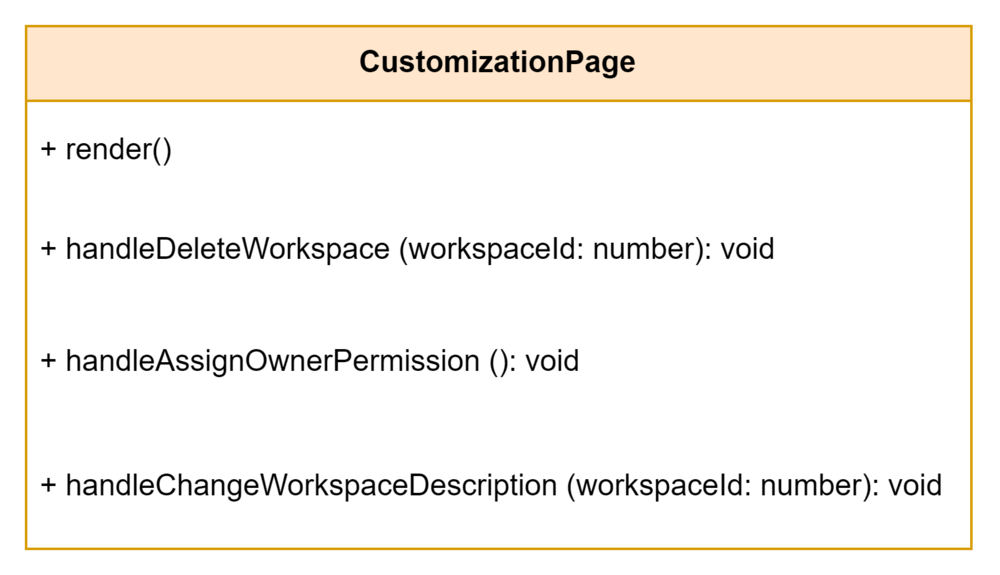
\includegraphics[ width = 0.5\linewidth]{Content/Phân tích và thiết kế hệ thống/documents/Sơ đồ lớp/images/Presentation layer/customizationPage.png}
    \vspace{0.5cm}
    \caption{Class CustomizationPage trong Presentation layer}
    \label{fig:Class CustomizationPage trong Presentation layer}
\end{figure}
Giao diện này sẽ hiện thực những chức năng dành cho người sở hữu workspace như xóa workspace, chuyển quyền sở hữu workspace cho thành viên khác hoặc thay đổi mô tả chi tiết của workspace.

\begin{figure}[H]
    \centering
    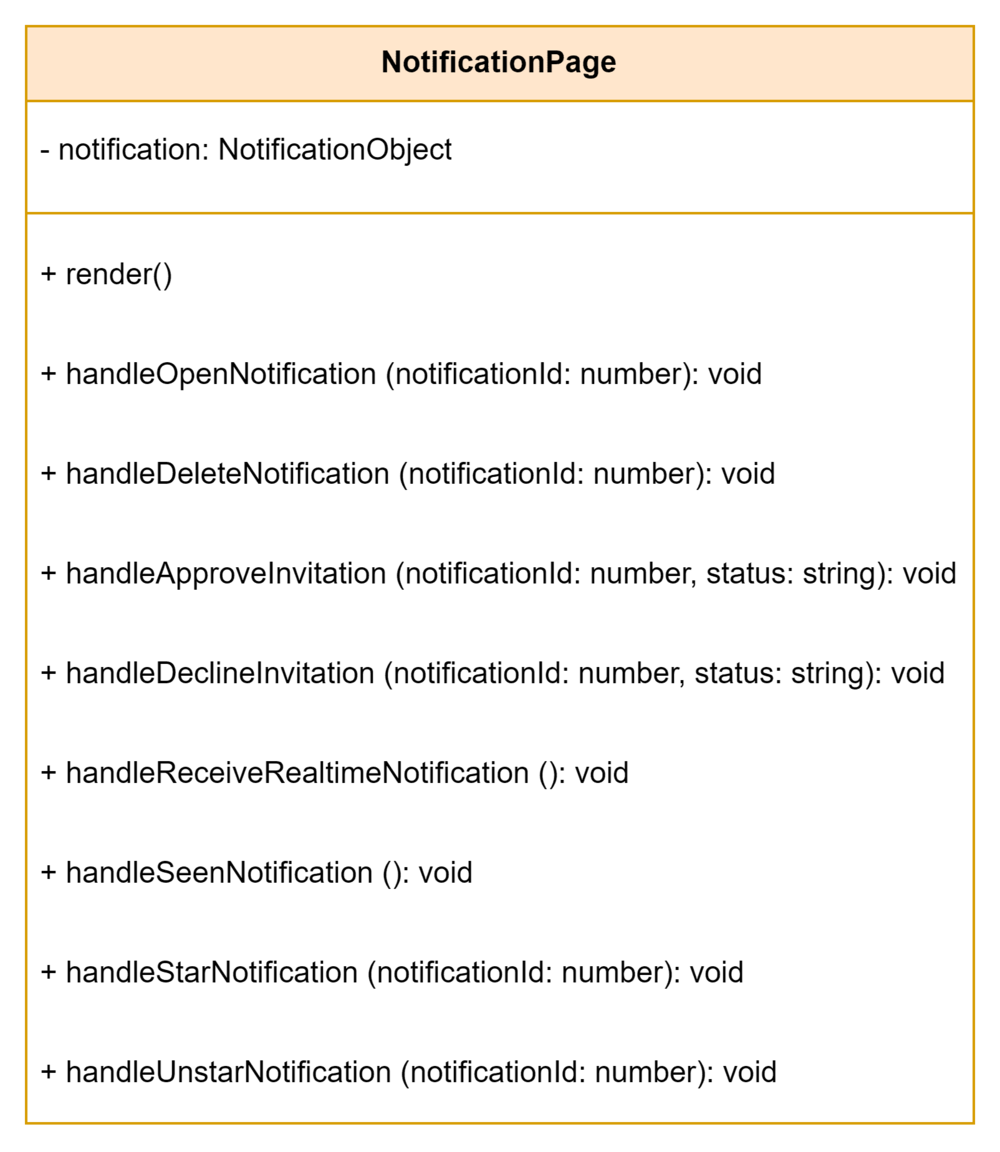
\includegraphics[ width = 0.5\linewidth]{Content/Phân tích và thiết kế hệ thống/documents/Sơ đồ lớp/images/Presentation layer/notificationPage.png}
    \vspace{0.5cm}
    \caption{Class NotificationPage trong Presentation layer}
    \label{fig:Class NotificationPage trong Presentation layer}
\end{figure}
Giao diện thông báo cá nhân là giao diện phụ trách việc hiển thị và giúp người dùng phản hồi những thông báo gửi đến họ. Sẽ có nhiều loại thông báo nhưng trong đó sẽ có thông báo yêu cầu xác nhận từ người dùng (lời mời vào workspace của thành viên trong workspace), hệ thống còn ghi nhận những thông báo đã được đọc và trạng thái của chúng để giúp người dùng có trải nghiệm tốt hơn khi truy xuất những thông báo cần xử lý.

\subsubsection{Business Layer}

\begin{figure}[H]
    \centering
    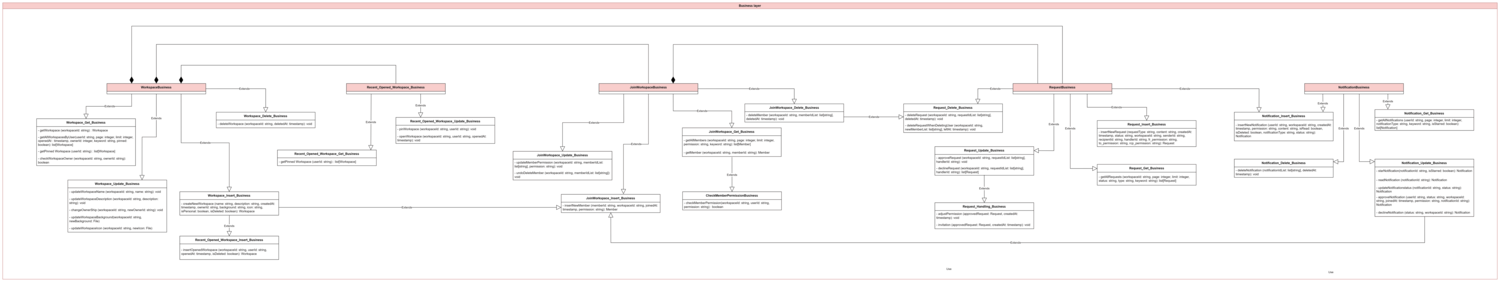
\includegraphics[ width = \linewidth]{Content/Phân tích và thiết kế hệ thống/documents/Sơ đồ lớp/images/Business layer/businessLayer.png}
    \vspace{0.5cm}
    \caption{Business Layer}
    \label{fig:Business Layer}
\end{figure}

Nhiệm vụ của tầng Business là phân tích những yêu cầu, xử lý logic nghiệp vụ và
gọi tới các đối tượng ở tầng Persistence để tương tác với cơ sở dữ liệu.

\begin{figure}[H]
    \centering
    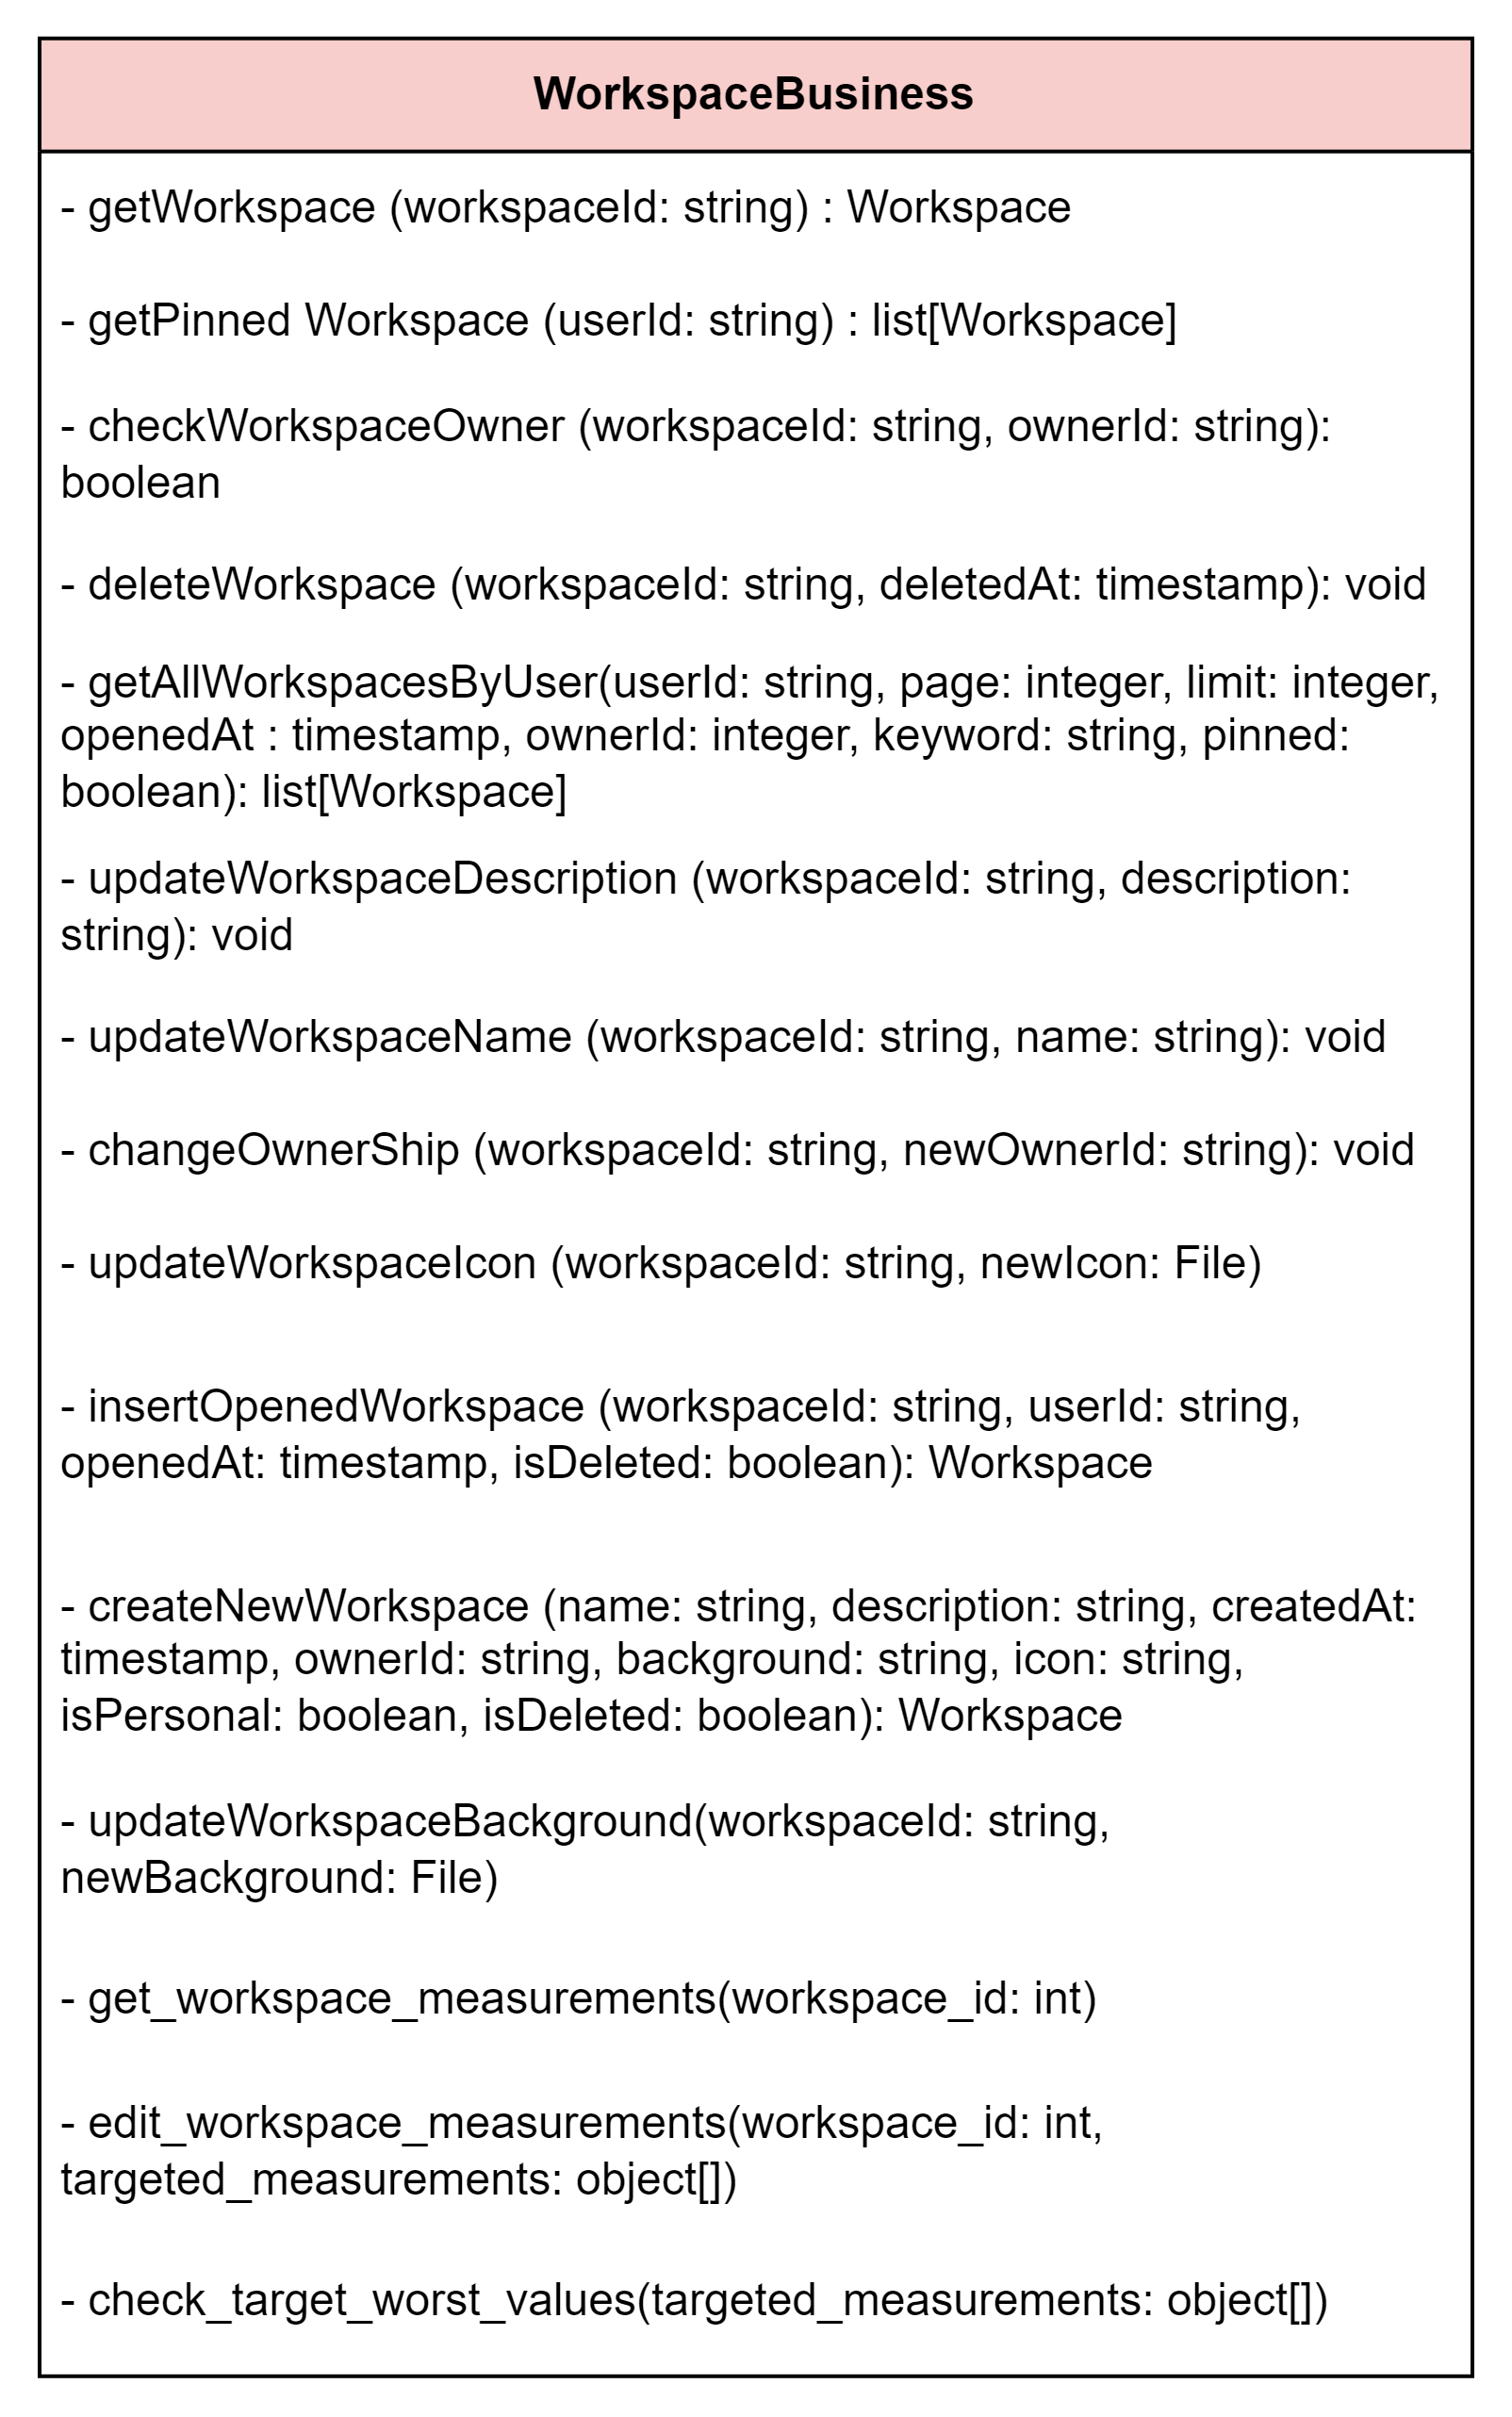
\includegraphics[ width = \linewidth]{Content/Phân tích và thiết kế hệ thống/documents/Sơ đồ lớp/images/Business layer/workspaceBusiness.png}
    \vspace{0.5cm}
    \caption{Workspace Business}
    \label{fig:Workspace Business}
\end{figure}

\begin{figure}[H]
    \centering
    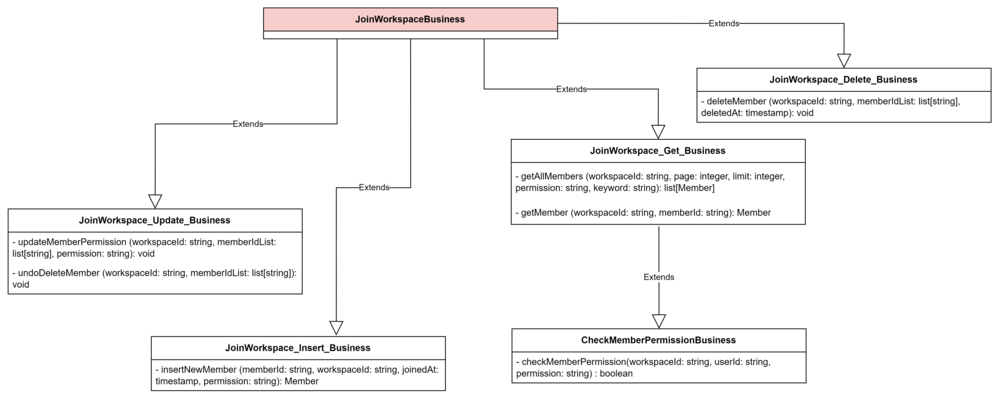
\includegraphics[ width = \linewidth]{Content/Phân tích và thiết kế hệ thống/documents/Sơ đồ lớp/images/Business layer/joinWorkspaceBusiness.png}
    \vspace{0.5cm}
    \caption{Join Workspace Business}
    \label{fig:Join Workspace Business}
\end{figure}

\begin{figure}[H]
    \centering
    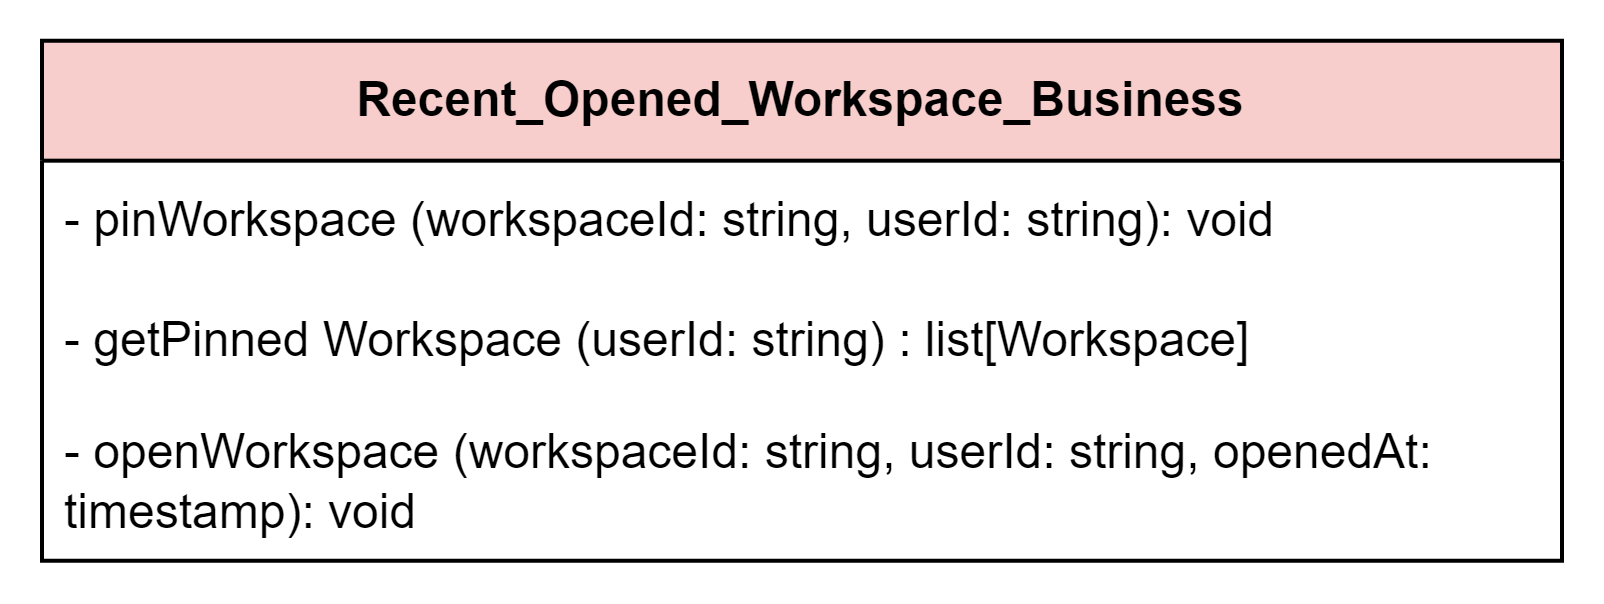
\includegraphics[ width = \linewidth]{Content/Phân tích và thiết kế hệ thống/documents/Sơ đồ lớp/images/Business layer/recentOpenedWorkspaceBusiness.png}
    \vspace{0.5cm}
    \caption{Recent Opened Workspace Business}
    \label{fig:Recent Opened Workspace Business}
\end{figure}

\begin{figure}[H]
    \centering
    \includegraphics[ width = \linewidth]{Content/Phân tích và thiết kế hệ thống/documents/Sơ đồ lớp/images/Business layer/requestBusiness.png}
    \vspace{0.5cm}
    \caption{Request Business}
    \label{fig:Request Business}
\end{figure}

\begin{figure}[H]
    \centering
    \includegraphics[ width = \linewidth]{Content/Phân tích và thiết kế hệ thống/documents/Sơ đồ lớp/images/Business layer/notificationBusiness.png}
    \vspace{0.5cm}
    \caption{Notification Business}
    \label{fig:Notification Business}
\end{figure}



\subsection{Persistence Layer}

\begin{figure}[H]
    \centering
    \includegraphics[ width = \linewidth]{Content/Phân tích và thiết kế hệ thống/documents/Sơ đồ lớp/images/Persistence layer/persistenceLayer2.png}
    \vspace{0.5cm}
    \caption{Tổng quan Persistence Layer}
    \label{fig:Tổng quan Persistence Layer}
\end{figure}
Tầng Persistence sẽ nhận dữ liệu, yêu cầu từ tầng Business để thực hiện các thao tác tương tác với cơ sở dữ liệu, sau đó trả về kết quả cho tầng Business.
Các class ở tầng Business sẽ có các class ở tầng Persistence tương ứng để thực hiện xử lý dữ liệu.

% \begin{figure}[H]
%     \centering
%     \includegraphics[ width = \linewidth]{Content/Phân tích và thiết kế hệ thống/documents/Sơ đồ lớp/images/Persistence layer/workspacePersistence.png}
%     \vspace{0.5cm}
%     \caption{Class WorkspacePersistence trong Persistence layer}
%     \label{fig:Class WorkspacePersistence trong Persistence layer}
% \end{figure}
% \par
% Class WorkspacePersistence sẽ chịu trách nhiệm thao tác với cơ sở dữ liệu 
% liên quan đến bảng Workspace. Class này sẽ thừa kế các class khác như:
% Workspace\_Get\_Persistence, Workspace\_Delete\_Persistence, Workspace\_Update\_Persistence.
% Những class này sẽ thực hiện các chức năng tương ứng với tên của chúng.
% \begin{figure}[H]
%     \centering
%     \includegraphics[ width = \linewidth]{Content/Phân tích và thiết kế hệ thống/documents/Sơ đồ lớp/images/Persistence layer/joinWorkspacePersistence.png}
%     \vspace{0.5cm}
%     \caption{Class JoinWorkspacePersistence trong Persistence layer}
%     \label{fig:Class JoinWorkspacePersistence trong Persistence layer}
% \end{figure}
% \par
% Class Join\_Workspace\_Persistence sẽ chịu trách nhiệm thao tác với cơ sở dữ liệu
% liên quan đến bảng Join\_Workspace. Class này sẽ thừa kế các class khác như:
% Join\_Workspace\_Get\_Persistence, Join\_Workspace\_Delete\_Persistence, Join\_Workspace\_Update\_Persistence.
% \begin{figure}[H]
%     \centering
%     \includegraphics[ width = \linewidth]{Content/Phân tích và thiết kế hệ thống/documents/Sơ đồ lớp/images/Persistence layer/recentOpenedWorkspacePersistence.png}
%     \vspace{0.5cm}
%     \caption{Class RecentOpenedWorkspacePersistence trong Persistence layer}
%     \label{fig:Class RecentOpenedWorkspacePersistence trong Persistence layer}
% \end{figure}
% \par
% Class Recent\_Opened\_Workspace\_Persistence sẽ chịu trách nhiệm thao tác với cơ sở dữ liệu
% liên quan đến bảng Recent\_Opened\_Workspace. Class này sẽ thừa kế các class khác như:
% Recent\_Opened\_Workspace\_Get\_Persistence, Recent\_Opened\_Workspace\_Update\_Persistence.
% \begin{figure}[H]
%     \centering
%     \includegraphics[ width = \linewidth]{Content/Phân tích và thiết kế hệ thống/documents/Sơ đồ lớp/images/Persistence layer/requestPersistence.png}
%     \vspace{0.5cm}
%     \caption{Class RequestPersistence trong Persistence layer}
%     \label{fig:Class RequestPersistence trong Persistence layer}
% \end{figure}
% \par
% Class Request\_Persistence sẽ chịu trách nhiệm thao tác với cơ sở dữ liệu
% liên quan đến bảng Request. Class này sẽ thừa kế các class khác như:
% Request\_Get\_Persistence, Request\_Delete\_Persistence, Request\_Update\_Persistence, Request\_Insert\_Persistence.
% \begin{figure}[H]
%     \centering
%     \includegraphics[ width = \linewidth]{Content/Phân tích và thiết kế hệ thống/documents/Sơ đồ lớp/images/Persistence layer/notificationPersistence.png}
%     \vspace{0.5cm}
%     \caption{Class NotificationPersistence trong Persistence layer}
%     \label{fig:Class NotificationPersistence trong Persistence layer}
% \end{figure}
% \par
% Class Notification\_Persistence sẽ chịu trách nhiệm thao tác với cơ sở dữ liệu
% liên quan đến bảng Notification. Class này sẽ thừa kế các class khác như:
% Notification\_Get\_Persistence, Notification\_Delete\_Persistence, Notification\_Update\_Persistence, Notification\_Insert\_Persistence.
\subsection{Thiết kế cơ sở dữ liệu}
\subsubsection{Lược đồ ERD}
\begin{figure}[H]
        \centering
        \includegraphics[width=\linewidth]{Content/Phân tích và thiết kế hệ thống/images/erd.png}
        \caption{Lược đồ ERD}
        \label{fig:Lược đồ ERD}
\end{figure}
\subsubsection{Ánh xạ ERD và mô tả chi tiết thực thể}
\paragraph{User: Người dùng của hệ thống}
\begin{center}
\begin{tabular}{|p{3cm} |p{2cm} |p{9cm}|}
 \hline
    Thuộc tính & Kiểu & Mô tả \\ [0.5ex] 
 \hline
 \underline{ID} & integer & ID của người dùng. Khoá chính. \\ 
 \hline
 email & varchar & Email của người dùng \\
 \hline
 password & varchar & Mật khẩu của người dùng \\
 \hline
 phoneNumber & varchar & Số điện thoại của người dùng \\
 \hline
 name & text & tên người dùng \\ [1ex] 
 \hline
 avatar & text & Đường dẫn tới ảnh đại diện của người dùng \\
 \hline
 verified & boolean & True nếu tài khoản đã xác thực, False nếu tài khoản chưa xác thực \\
 \hline
\end{tabular}
\end{center}
\begin{figure}[h]
        \centering
        \includegraphics[width=\textwidth]{Content//Phân tích và thiết kế hệ thống//images//ERD_mapping/user_mapping.png}
        \label{fig:enter-label}
\end{figure}
\paragraph{Project: Dự án trong workspace}
\begin{center}
\begin{tabular}{ |p{4cm} |p{3cm} |p{7cm}|} 
 \hline
    Thuộc tính & Kiểu & Mô tả \\ [0.5ex] 
 \hline
 \underline{ID} & integer & ID của project. Khoá chính. \\ 
 \hline
 projectName & text & Tên của project \\
 \hline
 description & text & Mô tả của project \\
 \hline
 isDelete & boolean & Đánh dấu project này đã bị xoá hay chưa \\
 \hline
 createAt & timestamp & Thời gian project được tạo \\
 \hline
 ownerId & integer & ID của người sở hữu project.
 Khoá ngoại tham chiếu tới trường Id trong bảng User \\
 \hline
 workspaceId & integer & ID của workspace nơi mà project được tạo. Khoá ngoại tham chiếu tới trường Id trong bảng Workspace \\
 \hline
 deletedAt & timestamp & Thời gian project được xoá khỏi Workspace \\
 \hline
 isWorkspaceDeleted & boolean & Đánh dấu workspace đã bị xoá hay chưa \\
 \hline
\end{tabular}
\end{center}
\begin{figure}[h]
        \centering
        \includegraphics[width=\textwidth]{Content/Phân tích và thiết kế hệ thống/images/ERD_mapping/project_mapping.png}
        \label{fig:enter-label}
\end{figure}

\paragraph{Workspace: Không gian làm việc trong hệ thống}
\begin{center}
\begin{tabular}{ |p{2cm} |p{3cm} |p{9cm}|} 
 \hline
    Thuộc tính & Kiểu & Mô tả \\ [0.5ex] 
 \hline
 \underline{ID} & integer & ID của workspace. Khoá chính. \\ 
 \hline
 name & text & Tên của workspace \\
 \hline
 description & text & Mô tả của workspace \\
 \hline
 isDeleted & boolean & Đánh dấu workspace đã bị xoá hay chưa \\
 \hline
 createAt & timestamp & Thời gian workspace được tạo \\
 \hline
 ownerId & integer & ID của người sở hữu workspace.
 Khoá ngoại tham chiếu tới trường Id trong bảng User \\
 \hline
 background & text & Đường link dẫn tới background của workspace \\
 \hline
 icon & text & Đường link dẫn tới icon của workspace \\
 \hline
 deletedAt & timestamp & Thời gian Workspace được xoá khỏi hệ thống \\
 \hline
 isPersonal & boolean & True nếu đây là workspace cá nhân. False nếu là workspace khác \\
 \hline
\end{tabular}
\end{center}
\begin{figure}[h]
        \centering
        \includegraphics[width=\textwidth]{Content/Phân tích và thiết kế hệ thống/images/ERD_mapping/joinWorkspace_mapping.png}
        \label{fig:enter-label}
\end{figure}

\paragraph{Join Workspace: Quan hệ tham gia giữa người dùng và workspace}
\begin{center}
\begin{tabular}{ |p{3cm} |p{2cm} |p{9cm} |} 
 \hline
    Thuộc tính & Kiểu & Mô tả \\ [0.5ex] 
 \hline
 \underline{memberId} & integer & ID của member tham gia Workspace. Khoá ngoại tham chiếu tới trường Id trong User. \\ 
 \hline
 \underline{workspaceId} & integer & ID của Workspace. Khoá ngoại tham chiếu tới trường Id trong Workspace. \\
 \hline
 joinedAt & timestamp & Thời gian người dùng tham gia Workspace \\
 \hline
 isDeleted & boolean & Đánh dấu người dùng đã rời khỏi Workspace hay chưa \\
 \hline
 permission & text & Quyền hạn của người dùng khi tham gia Workspace \\
 \hline
 leftAt & timestamp & Thời gian người dùng rời khỏi Workspace \\
 \hline
 isWorkspaceDeleted & boolean & Đánh dấu workspace đã bị xoá hay chưa \\
 \hline
\end{tabular}
\end{center}
\begin{figure}[h]
        \centering
        \includegraphics[width=\textwidth]{Content/Phân tích và thiết kế hệ thống/images/ERD_mapping/joinWorkspace_mapping.png}
        \label{fig:enter-label}
\end{figure}

\paragraph{Recent Opened Workspace: Quan hệ chỉnh sửa giữa người dùng và workspace}
\begin{center}
\begin{tabular}{ |p{3cm} |p{2cm} |p{9cm}|} 
 \hline
    Thuộc tính & Kiểu & Mô tả \\ [0.5ex] 
 \hline
 \underline{userId} & integer & ID của member tham gia Workspace. Khoá ngoại tham chiếu tới trường Id trong User. \\ 
 \hline
 \underline{workspaceId} & integer & ID của Workspace. Khoá ngoại tham chiếu tới trường Id trong Workspace. \\
 \hline
 openedAt & timestamp & Thời gian người dùng mở Workspace lần cuối.\\
 \hline
 isHided & boolean & Đánh dấu người dùng đã ẩn Workspace khỏi danh sách của mình hay chưa \\
 \hline
 isPinned & boolean & Đánh dấu người dùng đã pin Workspace vào danh sách ưu tiên hay chưa \\
 \hline
 isWorkspaceDeleted & boolean & Đánh dấu workspace đã bị xoá hay chưa \\
 \hline
\end{tabular}
\end{center}
\begin{figure}[h]
        \centering
        \includegraphics[width=\textwidth]{Content/Phân tích và thiết kế hệ thống/images/ERD_mapping/recent_opened_workspace_mapping.png}
        \label{fig:enter-label}
\end{figure}

\paragraph{Request: Các yêu cầu trong hệ thống}
\begin{center}
\begin{tabular}{ |p{3cm} |p{3cm} |p{9cm}|} 
 \hline
    Thuộc tính & Kiểu & Mô tả \\ [0.5ex] 
 \hline
 \underline{ID} & integer & ID của request. Khoá chính \\ 
 \hline
 type & varchar & Kiểu request \\
 \hline
 createdAt & timestamp & Thời gian người dùng tạo request.\\
 \hline
 status & text & Trạng thái của request, đang được xử lý hay đã được chấp thuận, từ chối.\\
 \hline
 isDeleted & boolean & Đánh dấu request bị xoá hay chưa \\
 \hline
 isWorkspaceDeleted & boolean & Đánh dấu workspace đã bị xoá hay chưa \\
 \hline
 workspaceId & integer & ID của workspace chứa request đó. Khoá ngoại tham chiếu tới trường Id trong Workspace \\
 \hline
  senderId & integer & ID của người gửi request. Khoá ngoại tham chiếu tới trường Id trong User \\
 \hline
  recipientId & integer & ID của người nhận request đã xử lý. Khoá ngoại tham chiếu tới trường Id trong User \\
 \hline
  handlerId & integer & ID của người xử lý request. Khoá ngoại tham chiếu tới trường Id trong User \\
 \hline
  frPermission & text & permission hiện tại của người gửi. \\
 \hline
  toPermission & text & permission mong muốn của người gửi. \\
 \hline
  rcpPermission & text & permission của người sẽ nhận được lời mời tham gia workspace. \\
 \hline
  deletedAt & timestamp & Thời gian xoá request. \\
 \hline
\end{tabular}
\end{center}
\begin{figure}[h]
        \centering
        \includegraphics[width=\textwidth]{Content/Phân tích và thiết kế hệ thống/images/ERD_mapping/request_mapping.png}
        \label{fig:enter-label}
\end{figure}

\paragraph{Notification: Các thông báo của người dùng}
\begin{center}
\begin{tabular}{ |p{3cm} |p{3cm} |p{9cm}|} 
 \hline
    Thuộc tính & Kiểu & Mô tả \\ [0.5ex] 
 \hline
 \underline{ID} & integer & ID của thông báo. Khoá chính \\ 
 \hline
 notificationType & varchar & Kiểu thông báo \\
 \hline
 createdAt & timestamp & Thời gian người dùng nhận được thông báo.\\
 \hline
 status & text & Trạng thái của thông báo, đã được chấp thuận hay đồng ý hoặc từ chối lời mời.\\
 \hline
 isDeleted & boolean & Đánh dấu thông báo bị xoá hay chưa \\
 \hline
 isStarred & boolean & Đánh dấu thông báo đã được đánh dấu ưu tiên hay chưa \\
 \hline
 workspaceId & integer & ID của workspace gửi thông báo đó. Khoá ngoại tham chiếu tới trường Id trong Workspace \\
 \hline
  isRead & boolean & Đánh dấu thông báo đã được đọc hay chưa \\
 \hline
  permission & text & permission của người nhận. \\
 \hline
  deletedAt & timestamp & Thời gian xoá request. \\
 \hline
\end{tabular}
\end{center}
\begin{figure}[h]
        \centering
        \includegraphics[width=\textwidth]{Content/Phân tích và thiết kế hệ thống/images/ERD_mapping/notification_mapping.png}
        \label{fig:enter-label}
\end{figure}
\newpage
\chapter{Hiện thực hệ thống}
\subsection{Công nghệ sử dụng}
\subsubsection{ReactJS}
React là một thư viện Javascript mã nguồn mở, được phát triển và hỗ trợ bởi
Meta (trước đây là Facebook), ra mắt vào năm 2013 với mục đích xây dựng giao
diện người dùng. React được sử dụng rộng rãi để xây dựng các trang web \acrfull*{spa} và các ứng dụng trên nền tảng di động. React tổ chức
các thành phần của trang web thành các component, cho phép chúng ta nhóm các
logic xử lý của các phần nhỏ của giao diện lại với nhau, từ đó có thể tái sử
dụng nhiều lần và mở rộng thêm chức năng cho mỗi thành phần đó. Mỗi component
có thể tự quản lý trạng thái (state) của riêng mình, cũng như nhận vào các
thuộc tính (props) được truyền từ component cha. React tối ưu việc render trang
web bằng cách chỉ cho phép render khi phát hiện có sự thay đổi trong state và
props, từ đó giảm thiểu số lần phải re - render. React còn nổi tiếng với việc
sử dụng Virtual \acrshort*{dom} để cải thiện hiệu năng, khi so sánh DOM gốc của trang web
và Virtual DOM để tìm ra những sự khác nhau, và chỉ render lại những điểm khác
nhau đó, thay vì re - render cả cây DOM, điều mà sẽ làm hiệu năng của trang web
giảm đi đáng kể.
\par
Một số ưu điểm của React có thể kể đến như sau:
\begin{itemize}
    \item Cập nhật hiệu quả. Các thuật toán của ReactJS đảm bảo rằng các cập nhật, thay
          đổi UI được thực thi hiệu quả. Chỉ những components bị ảnh hưởng bởi một thay
          đổi nào đó mới được re - render, giúp tối ưu hoá tổng quan hiệu năng của ứng
          dụng.
    \item Luồng dữ liệu một chiều. ReactJS chỉ cung cấp luồng dữ liệu đi theo một chiều,
          giúp cho lập trình viên dễ dàng hiểu cách dữ liệu hoạt động, thay đổi như thế
          nào trong cây phân cấp component, cũng như dự đoán trước trạng thái của
          component.
    \item Cộng đồng lớn. ReactJS là thư viện front-end Javascript nổi tiếng, do đó sự hỗ
          trợ từ cộng đồng là rất tốt khi ta có vấn đề trong việc lập trình. Ngoài ra,
          các thư viện, components của bên thứ ba, các hooks được phát triển và duy trì
          bởi hàng triệu lập trình viên trên toàn thế giới, giúp ta có thể tìm thấy thư
          viện mong muốn, phục vụ cho các chức năng khác nhau của hệ thống.
\end{itemize}
\subsubsection{Python}
Kế thừa từ đề tài trước, ở đề tài này, nhóm tiếp tục sử dụng Python làm ngôn
ngữ lập trình chính cho phần server của hệ thống và áp dụng framework Flask.
\par
Ở Flask có một số ưu điểm nổi bật để chúng tôi quyết định lựa chọn nó:
\begin{itemize}
    \item Flask là một micro web framework được viết bằng Python, không yêu cầu tool hay
          thư viện cụ thể nào. “Micro” không có nghĩa là thiếu chức năng mà “micro” theo
          triết lý thiết kế là cung cấp một lõi chức năng “súc tích” nhất cho ứng dụng
          web nhưng người dùng có thể mở rộng bất cứ lúc nào. Flask luôn hỗ trợ các thành
          phần tiện ích mở rộng cho ứng dụng như tích hợp cơ sở dữ liệu, xác thực biểu
          mẫu, xử lý upload, các công nghệ xác thực, template, email, RESTful... Người
          dùng có thể tập trung xây dựng web application ngay từ đầu trong một khoảng
          thời gian rất ngắn và có thể mở rộng quy mô của ứng dụng tùy theo yêu cầu.
    \item Chính nguyên lý và áp dụng microframework đã giúp cho Flask Python có thể dễ
          dàng mở rộng nếu có nhu cầu từ ứng dụng web. Do phần core chạy độc lập và ít
          phụ thuộc, nên cho dù mở rộng ở mức quy mô thì ứng dụng web sử dụng Flask
          Python vẫn đáp ứng được.
    \item Sự linh hoạt là tính năng cốt lõi và cũng là ưu điểm của Flask Python. Chính vì
          giữ cho core và các thành phần khác đơn giản nên ít bị phụ thuộc vào nhau, sự
          đơn giản này giúp ta có thể chuyển hướng ứng dụng web theo business owner dễ
          dàng hơn. Ngoài ra do ít bị phụ thuộc lẫn nhau nên một thành phần nào đó bị sập
          cũng khó mà kéo theo cả hệ thống bị sập.
\end{itemize}
\subsubsection{Websocket và Socket.IO}
Websocket là một công nghệ theo thời gian thực, cung cấp một giao tiếp hai
chiều, song công toàn phần giữa máy khách và máy chủ trên một kết nối đơn
socket, bền vững. Trong chế độ truyền song công toàn phần, việc giao tiếp giữa
bên gửi và bên nhận có thể diễn ra đồng thời, bên gửi và bên nhận có thể truyền
và nhận tín hiệu cùng một lúc. Chế độ truyền song công toàn phần giống như con
đường hai chiều, trong đó các phương tiện có thể lưu chuyển theo cả hai hướng
cùng một lúc. Ví dụ, trong một cuộc trò chuyện qua điện thoại, hai người giao
tiếp và cả hai có thể tự do nói và nghe cùng một lúc. Một kết nối Websocket sẽ
bắt đầu với một HTTP request/response handshake. Nếu handshake khởi tạo thành
công, máy chủ và máy khách đồng ý sử dụng kết nối \acrshort*{tcp} có sẵn đã được thiết lập
cho một kết nối Websocket. Kết nối này sẽ tồn tại lâu nhất có thể (theo lý
thuyết có thể tồn tại mãi mãi), cho phép máy chủ và máy khách có thể độc lập
gửi dữ liệu cho nhau.
\par
Một số ưu điểm của Websocket:
\begin{itemize}
    \item Trước khi có Websocket, các kỹ thuật \acrshort*{http} như \acrshort*{ajax} long polling và Comet là
          những tiêu chuẩn để xây dựng các ứng dụng thời gian thực. Tuy nhiên, ở
          Websocket đã lược bỏ đi việc thiết lập kết nối mỗi khi có request, và giảm kích
          thước của mỗi message vì không còn HTTP headers. Điều này giúp tiết kiệm băng
          thông, cải thiện độ trễ.
    \item Độ linh hoạt đã ăn sâu vào thiết kế của công nghệ Websocket, cho phép việc hiện thực các giao thức ở tầng ứng dụng và các mở rộng cho những chức năng khác (ví dụ như pub/sub messaging).
    \item Là một công nghệ hướng sự kiện (event - driven), Websocket cho phép dữ liệu
          được truyền đi mà không cần máy khách phải gửi request. Cơ chế này sẽ cực kỳ
          hữu ích trong ngữ cảnh máy khách cần phản ứng nhanh chóng với một sự kiện nào
          đó (đặc biệt là những sự kiện không thể dự đoán trước).
\end{itemize}
\par
Dẫu vậy, Websocket vẫn có một số những nhược điểm như sau:
\begin{itemize}
    \item Không như HTTP, Websocket là có trạng thái (stateful). Trong một số trường hợp
          sẽ khá khó khăn khi phải xử lý điều này, đặc biệt là lúc mở rộng hệ thống, bởi
          vì nó yêu cầu phía server phải theo dõi mỗi kết nối Websocket đơn lẻ và duy trì
          các thông tin trạng thái.
    \item Websocket không tự động khôi phục khi các kết nối bị huỷ - và để tự động khôi
          phục ta cần phải tự hiện thực tính năng này. Đây cũng là lý do vì sao có nhiều
          thư viện hỗ trợ Websocket phía máy khách.
    \item Một số môi trường (ví dụ như môi trường trong doanh nghiệp với các proxy
          servers) sẽ chặn các kết nối Websocket.
\end{itemize}
\par
Chính vì vậy, chúng tôi sử dụng thêm một thư viện để hỗ trợ trong việc trao đổi
dữ liệu qua giao thức Websocket. Socket.IO là một thư viện theo thời gian thực,
giúp giảm thiểu độ trễ và giao tiếp hai chiều giữa máy khách và mát chủ.
Socket.IO được xây dựng trên nền tảng giao thức Websocket, và cung cấp thêm một
số tính năng khác như tự động kết nối lại, hỗ trợ broadcast,...
\par
Một số ưu điểm của Socket.IO:
\begin{itemize}
    \item Socket.IO hỗ trợ multiplexing thông qua namespaces. Việc tận dụng namespaces
          giúp ta có thể tối giản hoá số lượng kết nối TCP đã sử dụng, và lưu các cổng
          socket trên máy chủ.
    \item Socket.IO cho phép phía máy chủ có thể linh hoạt broadcast các sự kiện đến tất
          cả máy khách đã kết nối. Ta cũng có thể broadcast các sự kiện tới một tập nhỏ
          các máy khách thông qua tính năng room.
    \item Socket.IO hỗ trợ HTTP long polling như một phương án dự phòng, sẽ hữu ích trong
          các môi trường không hỗ trợ Websocket.
    \item Socket.IO cung cấp cơ chế Ping/Pong, cho phép phát hiện một kết nối có đang
          hoạt động hay không. Ngoài ra, nếu một máy khách bị ngắt kết nối, nó sẽ tự động
          kết nối lại.
\end{itemize}
Tuy nhiên, thư viện này cũng bộc lộ một số nhược điểm như sau:
\begin{itemize}
    \item Socket.IO có giới hạn trong các tính năng bảo mật. Chẳng hạn như, nó không cung
          cấp mã hoá đầu cuối, hay cơ chế nào để tạo ra và làm mới các tokens phục vụ cho
          việc xác thực người dùng.
    \item Không tương thích với những hiện thực Websocket khác. Ta không thể sử dụng một
          máy khách Websocket cơ bản với một máy chủ Socket.IO.
    \item Socket.IO được thiết kế để làm việc trong một vùng đơn, hơn là kiểu kiến trúc
          đa vùng. Điều này có thể làm gia tăng độ trễ nếu các người dùng ở các vùng khác
          nhau.
\end{itemize}
\par
Mặc dù Socket.IO có một số nhược điểm như trên, chúng tôi nhận thấy rằng những
nhược điểm đó không ảnh hưởng nhiều đến hệ thống, và những ưu điểm của
Socket.IO là đủ để chúng tôi quyết định sử dụng nó.

\subsubsection{PostgreSQL}
Để thiết kế database cho mục đích lưu trữ dữ liệu, nhóm quyết định chọn cơ sở
dữ liệu quan hệ (relational database) để hiện thực, và hệ quản trị cơ sở dữ liệu
được chọn là PostgreSQL. Những lợi ích của việc sử dụng hệ cơ sở dữ liệu có quan
hệ như sau:
\begin{itemize}
    \item Bảo đảm tính toàn vẹn dữ liệu. Cơ sở dữ liệu quan hệ bắt buộc cần phải bảo đảm
          tính toàn vẹn dữ liệu, bằng việc sử dụng các ràng buộc như khoá chính, khoá
          ngoại, các ràng buộc duy nhất. Những ràng buộc này giúp cho dữ liệu được chính
          xác, nhất quán và tuân theo các quy định đã được định nghĩa từ trước.
    \item Nhờ việc sử dụng kỹ thuật chuẩn hoá dữ liệu, mà cơ sở dữ liệu quan hệ có thể
          tái tổ chức lại dữ liệu, lược bỏ những dư thừa hay các vấn đề liên quan đến
          nhất quán dữ liệu khi tiến hành chỉnh sửa, thêm, xoá dữ liệu.
    \item Hỗ trợ các công cụ cũng như tính năng nâng cao giúp người dùng dễ dàng xử lý
          trên dữ liệu một cách hiệu quả như indexing, transaction, cơ chế query
          optimization.
    \item Hệ quản trị cơ sở dữ liệu quan hệ cho phép lưu trữ và phục hồi nhờ việc cung
          cấp các cơ chế có sẵn cho việc phục hồi. Điều này đảm bảo dữ liệu có thể được
          lưu trữ một cách an toàn, giải quyết các vấn đề liên quan tới mất mát dữ liệu.
\end{itemize}
So sánh với các loại cơ sở dữ liệu không quan hệ phổ biến hiện nay, ưu điểm lớn nhất của việc sử dụng cơ sở dữ liệu quan hệ so với cơ sở dữ liệu không quan hệ trong phạm vi đề tài đó là việc sử dụng cấu trúc có quan hệ giúp quản lý dữ liệu tốt hơn, tính nhất quán dữ liệu được đảm bảo hơn. Ngoài ra, do đề tài này được phát triển dựa trên đề tài gốc vốn sử dụng cơ sở dữ liệu quan hệ, để đảm bảo tính thống nhất về mặt chức năng của hệ thống, nhóm nhận thấy tiếp tục loại hình cơ sở dữ liệu này là một điều đúng đắn.
\section{Hiện thực giao diện người dùng}

\subsection{Giao diện Trang chủ BPSky}

\begin{figure}[H]
    \centering
    \includegraphics[ width = 0.7\linewidth]{Content/Hiện thực hệ thống/documents/Hiện thực giao diện người dùng/images/DefaultHomepage.png}
    \vspace{0.5cm}
    \caption{Giao diện trang default homepage}
    \label{fig: Giao diện trang default homepage}
\end{figure}

Người dùng sau khi đăng nhập hệ thống thành công sẽ được chuyển hướng tới giao diện Default homepage. Tại giao diện mặc định này, hệ thống sẽ hiển thị hai danh sách "Recently opened workspace" - hiển thị danh sách những workspace người dùng tham gia/sở hữu theo thứ tự thời gian mở và "Pinned workspace" - hiển thị danh sách những workspace người dùng pin (đánh dấu). Người dùng có thể chọn icon "ba chấm" ở bên phải cùng của mỗi item để mở menu thao tác với mỗi item workspace.

\subsection{Giao diện tạo mới workspace}

% \begin{figure}[H]
%     \centering
%     \includegraphics[ width = 0.3\linewidth]{Content/Hiện thực hệ thống/documents/Hiện thực giao diện người dùng/images/DropdownMenu.png}
%     \vspace{0.5cm}
%     \caption{Dropdown menu}
%     \label{fig: Giao diện dropdown menu của mỗi item workspace}
% \end{figure}

\begin{figure}[H]
    \centering
    \includegraphics[ width = 0.7\linewidth]{Content/Hiện thực hệ thống/documents/Hiện thực giao diện người dùng/images/CreateModal.png}
    \vspace{0.5cm}
    \caption{Giao diện create modal khi người dùng tạo mới workspace}
    \label{fig: Giao diện create modal khi người dùng tạo mới workspace}
\end{figure}

Người dùng có thể tạo mới workspace bằng cách chọn "Create new workspace" từ dropdown menu. Sau khi chọn, hệ thống sẽ hiển thị giao diện create modal như hình \ref{fig: Giao diện create modal khi người dùng tạo mới workspace}. Tại đây, người dùng có thể nhập tên và mô tả cho workspace. Sau khi hoàn tất, người dùng có thể chọn "Create" để tạo mới workspace hoặc "Cancel" để hủy thao tác.

\subsection{Giao diện đổi tên workspace}

\begin{figure}[H]
    \centering
    \includegraphics[ width = \linewidth]{Content/Hiện thực hệ thống/documents/Hiện thực giao diện người dùng/images/RenameModal.png}
    \vspace{0.5cm}
    \caption{Giao diện rename modal khi người dùng đổi tên workspace}
    \label{fig: Giao diện rename modal khi người dùng đổi tên workspace}
\end{figure}

Người dùng có thể đổi tên workspace bằng cách chọn "Rename" từ dropdown menu. Sau khi chọn, hệ thống sẽ hiển thị giao diện rename modal như hình \ref{fig: Giao diện rename modal khi người dùng đổi tên workspace}. Tại đây, người dùng có thể nhập tên mới cho workspace. Sau khi hoàn tất, người dùng có thể chọn "Save" để đổi tên workspace hoặc "Cancel" để hủy thao tác.

\subsection{Giao diện chia sẻ workspace}

\begin{figure}[H]
    \centering
    \includegraphics[ width = 0.7\linewidth]{Content/Hiện thực hệ thống/documents/Hiện thực giao diện người dùng/images/ShareModal.png}
    \vspace{0.5cm}
    \caption{Giao diện share modal khi người dùng muốn mời/gửi yêu cầu mời người dùng khác vào workspace}
    \label{fig: Giao diện share modal khi người dùng muốn mời/gửi yêu cầu mời người dùng khác vào workspace}
\end{figure}

Người dùng có thể mời người dùng khác vào workspace bằng cách chọn "Share" từ dropdown menu. Sau khi chọn, hệ thống sẽ hiển thị giao diện share modal như hình \ref{fig: Giao diện share modal khi người dùng muốn mời/gửi yêu cầu mời người dùng khác vào workspace}. Tại đây, người dùng có thể nhập tên người dùng mà mình muốn mời vào workspace, sau đó chọn quyền hạn của người được mời vào - quyền hạn của người này không được phép cao hơn người gửi lời mời (owner > editor > sharer > viewer). Sau khi hoàn tất, người dùng có thể chọn "Share" để mời người dùng vào workspace hoặc "Cancel" để hủy thao tác.

\subsection{Giao diện thông tin chi tiết workspace}

\begin{figure}[H]
    \centering
    \includegraphics[ width = \linewidth]{Content/Hiện thực hệ thống/documents/Hiện thực giao diện người dùng/images/WorkspaceDetailPage.png}
    \vspace{0.5cm}
    \caption{Giao diện trang Workspace detail}
    \label{fig: Giao diện trang Workspace detail}
\end{figure}

Người dùng có thể truy cập vào trang Workspace detail bằng cách chọn vào tên của workspace từ danh sách các workspace mà người dùng đang tham gia/sở hữu. Tại đây, người dùng có thể xem danh sách những project có trong workspace. Tương tự với danh sách workspace, mỗi item project cũng sẽ có icon "ba chấm" ở phải cùng, người dùng có thể mở dropdown menu để thao tác với project.

\subsection{Giao diện thông báo của người dùng}

\begin{figure}[H]
    \centering
    \includegraphics[ width = 0.8\linewidth]{Content/Hiện thực hệ thống/documents/Hiện thực giao diện người dùng/images/NotificationPage.png}
    \vspace{0.5cm}
    \caption{Giao diện trang thông báo của người dùng}
    \label{fig: Giao diện trang thông báo của người dùng}
\end{figure}

Người dùng có thể truy cập vào trang thông báo bằng cách chọn icon hình chuông ở phía trên thanh điều hướng. Tại đây, người dùng có thể xem danh sách những thông báo mà hệ thống gửi tới người dùng. Mỗi item thông báo sẽ tùy thuộc vào loại thông báo tương ứng mà hiển thị trạng thái khác nhau (bao gồm "Approved" - chấp nhận, "Declined" - từ chối, "Pending" - đang chờ phản hồi). Người dùng có thể đánh dấu thông báo quan trọng bằng cách nhấn vào icon ngôi sao ở mỗi item thông báo, thông báo quan trọng có thể được lọc thông qua công cụ filter.

\subsection{Giao diện chi tiết thông báo của người dùng}

\begin{figure}[H]
    \centering
    \includegraphics[ width = \linewidth]{Content/Hiện thực hệ thống/documents/Hiện thực giao diện người dùng/images/NotificationDetailModal.png}
    \vspace{0.5cm}
    \caption{Giao diện modal hiển thị thông tin chi tiết của thông báo}
    \label{fig: Giao diện modal hiển thị thông tin chi tiết của thông báo}
\end{figure}

Người dùng có thể xem thông tin chi tiết của mỗi thông báo bằng cách nhấn vào item thông báo tương ứng. Hệ thống sẽ hiển thị giao diện modal như hình \ref{fig: Giao diện modal hiển thị thông tin chi tiết của thông báo}. Tại đây, người dùng có thể xem thông tin chi tiết của thông báo, tùy thuộc vào loại thông báo mà người dùng sẽ có thể tương tác "Approve" - chấp nhận hoặc "Decline" từ chối lời mời được đính kèm trong thông báo. Nếu người dùng muốn đóng modal, người dùng có thể nhấn vào nút "Cancel".

\subsection{Giao diện quản lý thành viên trong workspace}

\begin{figure}[H]
    \centering
    \includegraphics[ width = 0.8\linewidth]{Content/Hiện thực hệ thống/documents/Hiện thực giao diện người dùng/images/MembersManagementPage.png}
    \vspace{0.5cm}
    \caption{Giao diện trang quản lý thành viên trong Workspace}
    \label{fig: Giao diện trang quản lý thành viên trong Workspace}
\end{figure}

Nếu người dùng là người sở hữu workspace (workspace owner) thì có thể chọn icon bánh răng bên cạnh tên của workspace tại trang Workspace Detail để điều hướng tới giao diện quản lý workpsace. Người dùng sẽ được điều hướng mặc định tới trang quản lý thành viên trong workspace. Hệ thống sẽ hiển thị danh sách những thành viên có trong workspace cùng với quyền hạn và thời gian tham gia workspace của họ, chúng ta có thể lọc người dùng theo vai trò trong hệ thống. Nếu người sở hữu workspace muốn mời thêm thành viên trong hệ thống vào workspace thì có thể chọn nút "Invite", hệ thống sẽ mở Share modal - Share modal này sẽ gửi lời mời trực tiếp đến người dùng thông qua hòm thông báo.

\subsection{Giao diện quản lý yêu cầu từ thành viên trong workspace}

\begin{figure}[H]
    \centering
    \includegraphics[ width = \linewidth]{Content/Hiện thực hệ thống/documents/Hiện thực giao diện người dùng/images/RequestsManagementPage.png}
    \vspace{0.5cm}
    \caption{Giao diện trang quản lý yêu cầu từ thành viên trong workspace}
    \label{fig: Giao diện trang quản lý yêu cầu từ thành viên trong workspace}
\end{figure}

\begin{figure}[H]
    \centering
    \includegraphics[ width = \linewidth]{Content/Hiện thực hệ thống/documents/Hiện thực giao diện người dùng/images/RequestDetailModal.png}
    \vspace{0.5cm}
    \caption{Giao diện modal hiển thị thông tin chi tiết của yêu cầu}
    \label{fig: Giao diện modal hiển thị thông tin chi tiết của yêu cầu}
\end{figure}

Khi người dùng chọn "Request management" ở thanh sidebar thì hệ thống sẽ chuyển hướng người dùng tới trang quản lý yêu cầu của workspace. Tại đây, hệ thống sẽ hiển thị danh sách những yêu cầu được gửi từ phía thành viên bên trong workspace. Các yêu cầu từ phía thành viên sẽ được phân thành 2 loại: Yêu cầu điều chỉnh vai trò trong workspace và Yêu cầu mời thành viên bên ngoài vào workspace. Người dùng có thể chọn "Approve" hoặc "Decline" để phản hồi yêu cầu tương ứng. Nếu người dùng muốn xem thông tin chi tiết của yêu cầu, người dùng có thể nhấn vào item yêu cầu tương ứng, hệ thống sẽ hiển thị modal như hình \ref{fig: Giao diện modal hiển thị thông tin chi tiết của yêu cầu}.

\subsection{Giao diện quản lý process portfolio của workspace}

\begin{figure}[H]
    \centering
    \includegraphics[ width = 0.8\linewidth]{Content/Hiện thực hệ thống/documents/Hiện thực giao diện người dùng/images/ProcessPortfolio.png}
    \vspace{0.5cm}
    \caption{Giao diện quản lý process portfolio của workspace}
    \label{fig: Giao diện quản lý process portfolio của workspace}
\end{figure}

Sau khi người dùng chọn Process portfolio trên thanh điều hướng, hệ thống sẽ chuyển hướng người dùng tới trang quản lý/khởi tạo process portfolio cho workspace. Người dùng có thể thấy được danh sách những process version/project có trong workspace. Người dùng có thể chọn nút Process portfolio để xem biểu đồ process portfolio của workspace hoặc nút Performance level để chỉnh sửa các thông tin liên quan tới thang đo được sử dụng chung cho toàn bộ workspace.

\begin{figure}[H]
    \centering
    \includegraphics[ width = 0.8\linewidth]{Content/Hiện thực hệ thống/documents/Hiện thực giao diện người dùng/images/WorkspaceMeasurement.png}
    \vspace{0.5cm}
    \caption{Giao diện chỉnh sửa giá trị thang đo cho process portfolio của workspace}
    \label{fig: Giao diện chỉnh sửa giá trị thang đo cho process portfolio của workspace}
\end{figure}

Người dùng sẽ được yêu cầu nhập thông tin liên quan tới thang đo cho process portfolio của workspace. Sau khi nhập thông tin, người dùng có thể chọn nút Save để lưu thông tin hoặc nút Cancel để hủy bỏ thao tác. Thông tin này sẽ được sử dụng để xác định thang đo (giá trị lớn nhất, giá trị nhỏ nhất) khi tính toán những thông số liên quan tới hiệu suất của process version (Heatlh).

\begin{figure}[H]
    \centering
    \includegraphics[ width = 0.8\linewidth]{Content/Hiện thực hệ thống/documents/Hiện thực giao diện người dùng/images/ProcessVersionEdit.png}
    \vspace{0.5cm}
    \caption{Giao diện menu của process version}
    \label{fig: Giao diện menu của process version}
\end{figure}

Người dùng có thể chọn nút Edit trong menu trên item tương ứng để chỉnh sửa thông tin liên quan tới thang đo của process version. Sau khi chỉnh sửa xong, người dùng có thể chọn nút Save để lưu thông tin hoặc nút Cancel để hủy bỏ thao tác. Hoặc chọn Activate để kích hoạt process version tương ứng, mỗi một process chỉ có một version được đặt trạng thái active. Version này sẽ được sử dụng để khởi tạo biểu đồ process portfolio.

\begin{figure}[H]
    \centering
    \includegraphics[ width = 0.8\linewidth]{Content/Hiện thực hệ thống/documents/Hiện thực giao diện người dùng/images/ProcessVersionMeasurement.png}
    \vspace{0.5cm}
    \caption{Giao diện chỉnh sửa giá trị của process version trong workspace}
    \label{fig: Giao diện chỉnh sửa giá trị của process version trong workspace}
\end{figure}

Nếu người dùng chọn Edit trong menu thì người dùng sẽ được yêu cầu nhập thông tin liên quan tới process version tương ứng. Hệ thống sẽ mở modal bao gồm thông tin về các giá trị Strategic importance (Mức độ quan trọng chiến lược), Feasibility (Tính khả thi) và Health (Hiệu suất) của version đó. Sau khi nhập thông tin, người dùng có thể chọn nút Save để lưu thông tin hoặc nút Cancel để hủy bỏ thao tác.

\begin{figure}[H]
    \centering
    \includegraphics[ width = 0.8\linewidth]{Content/Hiện thực hệ thống/documents/Hiện thực giao diện người dùng/images/ProcessPortfolioChart.png}
    \vspace{0.5cm}
    \caption{Giao diện biểu đồ process portfolio của workspace}
    \label{fig: Giao diện biểu đồ process portfolio của workspace}
\end{figure}

Người dùng sau khi chọn nút Process portfolio thì hệ thống sẽ mở biểu đồ process portfolio của workspace. Biểu đồ này sẽ hiển thị các process version/project có trong workspace. Mỗi node sẽ hiển thị thông tin liên quan tới process version tương ứng. Màu sắc của node sẽ thể hiện tính khả thi (Feasibility) của process version. Trục x và y sẽ lần lượt là giá trị của hiệu suất (Health) và mức độ quan trọng chiến lược (Strategic importance). Người dùng có thể di chuyển chuột qua node để xem thông tin chi tiết của process version tương ứng.

\begin{figure}[H]
    \centering
    \includegraphics[ width = 0.8\linewidth]{Content/Hiện thực hệ thống/documents/Hiện thực giao diện người dùng/images/NAProcessVersion.png}
    \vspace{0.5cm}
    \caption{Giao diện hiển thị danh sách process version không có/thiếu dữ liệu}
    \label{fig: Giao diện hiển thị danh sách process version không có/thiếu dữ liệu}
\end{figure}

Nếu có tồn tại process version nào trong workspace bị thiếu dữ liệu liên quan tới hiệu suất, tính khả thi hoặc độ quan trọng chiến lược thì hệ thống sẽ hiển thị danh sách những version đó. Người dùng cần bổ sung đầy đủ thông tin thì process portfolio mới được khởi tạo thành công.

\subsection{Giao diện khởi tạo khảo sát cho quy trình nghiệp vụ}

\begin{figure}[H]
    \centering
    \includegraphics[ width = \linewidth]{Content/Hiện thực hệ thống/documents/Hiện thực giao diện người dùng/images/Editor.png}
    \vspace{0.5cm}
    \caption{Giao diện chỉnh sửa mô hình quy trình nghiệp vụ}
    \label{fig: Giao diện chỉnh sửa mô hình quy trình nghiệp vụ}
\end{figure}

Khi người dùng muốn khởi tạo khảo sát cho quy trình đang làm việc hiện tại, người dùng cần mở quy trình tương ứng trong giao diện Editor, trên thanh công cụ (toolbar) người dùng chọn biểu tượng khảo sát (Launch Survey) để mở giao diện khởi tạo khảo sát.

\subsection{Giao diện chỉnh sửa nội dung khảo sát}

\begin{figure}[H]
    \centering
    \includegraphics[ width = \linewidth]{Content/Hiện thực hệ thống/documents/Hiện thực giao diện người dùng/images/SurveyBuilder.png}
    \vspace{0.5cm}
    \caption{Giao diện chỉnh sửa nội dung khảo sát}
    \label{fig: Giao diện chỉnh sửa nội dung khảo sát}
\end{figure}

Sau khi chọn biểu tượng khảo sát trên thanh công cụ thì người dùng sẽ được chuyển hướng tới trang giao diện chỉnh sửa nội dung bảng khảo sát. Giao diện chỉnh sửa nội dung khảo sát bao gồm các thành phần sau:

\begin{itemize}
    \item \textbf{Question configuration}: Người dùng có thể chỉnh sửa các thông tin của câu hỏi như tên câu hỏi, loại câu hỏi, câu trả lời (đối với loại câu hỏi multiple question), ...
    \item \textbf{Question item}: Hiển thị nội dung của câu hỏi và thứ tự của câu hỏi trong bảng khảo sát.
    \item \textbf{Question type}: Hiển thị phân loại của câu hỏi, trong phạm vi hệ thống có các loại câu hỏi như NPS, CES, CSAT, CES-IN và CES-IN (dùng thu thập ý kiến của người dùng), Multiple choice và Branching.
    \item \textbf{Delete question}: Dùng để xóa câu hỏi khỏi bảng khảo sát.
\end{itemize}

\subsection{Giao diện xem trước bảng khảo sát}

\begin{figure}[H]
    \centering
    \includegraphics[ width = 0.8\linewidth]{Content/Hiện thực hệ thống/documents/Hiện thực giao diện người dùng/images/SurveyPreview.png}
    \vspace{0.5cm}
    \caption{Giao diện xem trước bảng khảo sát}
    \label{fig: Giao diện xem trước bảng khảo sát}
\end{figure}

Người dùng có thể chọn nút Preview để mở phiên bản preview của bảng khảo sát.

\begin{figure}[H]
    \centering
    \includegraphics[ width = 0.8\linewidth]{Content/Hiện thực hệ thống/documents/Hiện thực giao diện người dùng/images/SurveyPreviewIntroduction.png}
    \vspace{0.5cm}
    \caption{Giao diện xem trước bảng khảo sát - trang mở đầu}
    \label{fig: Giao diện xem trước bảng khảo sát - trang mở đầu}
\end{figure}

Trang mở đầu của bảng khảo sát sẽ hiển thị thông tin chung của bảng khảo sát như tên, mô tả, những cảnh báo đối với người làm khảo sát. Để chuyển đến phần tiếp theo người dùng chọn nút Next, tương tự nếu muốn quay trở lại phần trước đó thì có thể chọn Back.

\begin{figure}[H]
    \centering
    \includegraphics[ width = 0.8\linewidth]{Content/Hiện thực hệ thống/documents/Hiện thực giao diện người dùng/images/SurveyPreviewConclusion.png}
    \vspace{0.5cm}
    \caption{Giao diện xem trước bảng khảo sát - trang kết thúc}
    \label{fig: Giao diện xem trước bảng khảo sát - trang kết thúc}
\end{figure}

Trang kết thúc của bảng khảo sát sẽ hiển thị lời cảm ơn và yêu cầu người dùng nhập thông tin như tên và email để nhận được kết quả của bảng khảo sát sau khi khảo sát đóng. Sau khi nhập đầy đủ thông tin thì người dùng chọn nút Submit để gửi đi phản hồi bảng khảo sát.

\subsection{Giao diện công bố khảo sát}

\begin{figure}[H]
    \centering
    \includegraphics[ width = 0.8\linewidth]{Content/Hiện thực hệ thống/documents/Hiện thực giao diện người dùng/images/SurveyPublish.png}
    \vspace{0.5cm}
    \caption{Giao diện công bố khảo sát}
    \label{fig: Giao diện công bố khảo sát}
\end{figure}

Sau khi người dùng hoàn thành việc cấu hình bảng khảo sát, người dùng có thể chọn mục Publish để công bố bảng khảo sát. Tại đây, người dùng có thể cấu hình các thông tin liên quan tới việc công bố bảng khảo sát như thời gian mở khảo sát, thời gian đóng khảo sát và email của người dùng được gửi thông báo khi khảo sát được mở. Ngoài ra người dùng có thể sử dụng url được tạo sẵn để mời người dùng khác tham gia khảo sát.

\subsection{Giao diện cấu hình khảo sát}

\begin{figure}[H]
    \centering
    \includegraphics[ width = 0.8\linewidth]{Content/Hiện thực hệ thống/documents/Hiện thực giao diện người dùng/images/SurveyGeneralConfiguration.png}
    \vspace{0.5cm}
    \caption{Giao diện cấu hình thông tin chung của bảng khảo sát}
    \label{fig: Giao diện cấu hình thông tin chung của bảng khảo sát}
\end{figure}

Người dùng sau khi chọn Configuration trên thanh điều hướng thì hệ thống sẽ chuyển hướng người dùng tới giao diện cấu hình thông tin chung của bảng khảo sát. Tại đây, người dùng có thể thay đổi các cấu hình liên quan tới bảng khảo sát như tên, mô tả và các trọng số của các loại câu hỏi trong bảng khảo sát. Các cấu hình này sẽ ảnh hưởng đến việc hiển thị và tính toán kết quả của bảng khảo sát.

\begin{figure}[H]
    \centering
    \includegraphics[ width = 0.8\linewidth]{Content/Hiện thực hệ thống/documents/Hiện thực giao diện người dùng/images/SurveyResponseConfiguration.png}
    \vspace{0.5cm}
    \caption{Giao diện cấu hình phản hồi của bảng khảo sát}
    \label{fig: Giao diện cấu hình phản hồi của bảng khảo sát}
\end{figure}

Ngoài ra, người dùng có thể chọn mục Survey response để chuyển hướng tới giao diện cấu hình phản hồi của bảng khảo sát. Tại đây, người dùng có thể cấu hình các thông tin liên quan tới phản hồi của bảng khảo sát như thông kết quả sau khi khảo sát hoàn thành qua hòm thư, cho phép người dùng thực hiện một/nhiều lần khảo sát và thời gian đóng/mở khảo sát.

\subsection{Giao diện kết quả bảng khảo sát}

\begin{figure}[H]
    \centering
    \includegraphics[ width = 0.8\linewidth]{Content/Hiện thực hệ thống/documents/Hiện thực giao diện người dùng/images/SurveyResult.png}
    \vspace{0.5cm}
    \caption{Giao diện kết quả bảng khảo sát}
    \label{fig: Giao diện kết quả bảng khảo sát}
\end{figure}

Sau khi người dùng chọn biểu tượng kết quả trên thanh công cụ thì hệ thống sẽ chuyển hướng người dùng tới trang giao diện kết quả bảng khảo sát. Giao diện này bao gồm kết quả thống kê chi tiết lựa chọn của từng câu hỏi trong bảng khảo sát và kết quả tổng hợp của bảng khảo sát. Tùy thuộc vào loại câu hỏi mà sẽ được thể hiện thông qua biểu đồ khác nhau:
\begin{itemize}
    \item Loại câu hỏi rẽ nhánh - Branching: Sử dụng biểu đồ tròn để thể hiện phần trăm số lượng câu trả lời cho từng lựa chọn Có/Không.
    \item Loại câu hỏi Multiple choice/CES/CSAT/NPS: Sử dụng biểu đồ cột để thể hiện phần trăm số lượng câu trả lời cho từng lựa chọn. Bao gồm có 7 lựa chọn (tương ứng từ 1 đến 7) đối với loại câu hỏi CES và CSAT, và 10 lựa chọn (tương ứng từ 0 đến 10) đối với loại câu hỏi NPS.
    \item Loại câu hỏi CES-IN/CSAT-IN: Sử dụng dạng danh sách câu trả lời ngắn để liệt kê những ý kiến của người làm khảo sát.
\end{itemize}
\section{Triển khai hệ thống}
Hiện nay có rất nhiều cách để triển khai của hệ thống phần mềm cho người dùng, sau đây là một số cách triển khai:
\begin{enumerate}
    \item Tự triển khai server: Đây là cách thủ công nhất để triển khai ứng dụng web, lập trình viên sẽ cài đặt các công cụ như web server (Apache, Nginx, IIS,...), database server (MySQL, PostgreSQL,...) và triển khai ứng dụng lên server của mình. Phương pháp này đòi hỏi kiến thức về quản trị hệ thống và bảo mật, tuy nhiên nó cung cấp cho lập trình viên sự linh hoạt cao để tùy chỉnh và điều khiển ứng dụng của mình.
    \item Platform-as-a-Service (PaaS): Đây là phương pháp triển khai ứng dụng web trên một nền tảng được quản lý bởi một nhà cung cấp dịch vụ. Lập trình viên chỉ cần đưa mã nguồn của ứng dụng lên nền tảng PaaS và các công cụ và hạ tầng sẽ được quản lý bởi nhà cung cấp dịch vụ. Các ví dụ về PaaS là Heroku, Google App Engine, Microsoft Azure và Amazon Web Services.
    \item Infrastructure-as-a-Service (IaaS): Đây là phương pháp triển khai ứng dụng web trên một hạ tầng đám mây được cung cấp bởi một nhà cung cấp dịch vụ. Lập trình viên có thể tự cấu hình môi trường của mình trên hạ tầng đám mây, bao gồm cả máy chủ ảo, lưu trữ, mạng và các công cụ khác. Các ví dụ về IaaS là Amazon Web Services, Google Cloud Platform và Microsoft Azure.
    \item Docker containers: Đây là phương pháp triển khai ứng dụng web trên các container Docker. Docker cho phép lập trình viên đóng gói ứng dụng và các phụ thuộc của nó trong một container, và triển khai các container này trên bất kỳ máy chủ nào. Phương pháp này đảm bảo tính di động và tương thích với mọi môi trường.
\end{enumerate}

Sau khi cân nhắc thì chúng tôi đã chọn cách tiếp cận là sử dụng PaaS để triển khai ứng dụng. Đây là một số ưu điểm cách tiếp cận này: 
\begin{enumerate}
    \item Tiết kiệm thời gian và chi phí: Không cần phải chi một khoản tiền lớn cho việc xây dựng, cài đặt phần cứng hay chi phí phát sinh trong khi hệ thống tạm ngừng hoạt động, và không phải tốn thời gian để thiết lập cũng như bảo trì phần lõi.
    \item Tăng tốc độ phát triển: Thiết lập và triển khai đơn giản, nhanh chóng đưa ứng dụng lên giai đoạn production.
    \item Mở rộng dễ dàng: Có thể mở rộng thêm về khả năng lưu trữ cũng như khả năng xử lý khi cần.
    \item Tính linh hoạt cao: cho phép các nhà phát triển có thể tham gia và làm việc trên các ứng dụng ở bất cứ nơi đâu.
\end{enumerate}
Tuy nhiên, PaaS cũng có một số hạn chế, như:
\begin{enumerate}
    \item Phụ thuộc vào nhà cung cấp dịch vụ: việc triển khai hệ thống trên các nền tảng này sẽ phụ thuộc khá nhiều vào khả năng của nhà cung cấp dịch vụ, chẳng hạn như băng thông, dung lượng,... Chỉ có thể chọn lựa những giải pháp có sẵn mà khó lòng tự điều chỉnh theo ý muốn và nhu cầu của nhà phát triển.
    \item Nguy cơ về bảo mật: Mặc dù các nhà cung cấp dịch vụ luôn cố gắng nâng cao và phát triển việc bảo mật nền tảng và cơ sở hạ tầng, vấn đề bảo mật của ứng dụng lại phụ thuộc khá nhiều vào mức độ bảo mật của nền tảng đó.
\end{enumerate}

\subsection{Triển khai phần Frontend của hệ thống}
\subsection{Triển khai phần Backend của hệ thống}
Việc triển khai ở phía backend của ứng dụng sử dụng nền tảng Render như sau:
\newline
Sau khi hoàn tất việc tạo tài khoản hoặc đăng nhập vào Render, chúng ta sẽ tạo một Web Service ở trên nền tảng này:
\begin{figure}[H]
    \centering
    \includegraphics[width=\linewidth]{Content/Hiện thực hệ thống/images/Webservice.png}
    \caption{Giao diện tạo Web service trên Render}
    \label{fig:Tạo Web service}
\end{figure}
Sau đó, ta thiết lập kết nối giữa service trên Render với nơi chứa source code. Ở đây, Render cung cấp 2 lựa chọn là kết nối với Repository trên Github hoặc một Image trên các nền tảng khác. Nhóm chúng tôi lựa chọn phương án đầu tiên.
\begin{figure}[H]
    \centering
    \includegraphics[width=\linewidth]{Content/Hiện thực hệ thống/images/gitrepo.png}
    \caption{Chọn kết nối với Repository}
    \label{fig:Chọn kết nối với Repository}
\end{figure}
Sau đó, chúng ta sẽ chọn kết nối đến một Repository cụ thể. Ở đây, chúng tôi chọn kết nối đến Repository BPE - be tương ứng với phần backend của hệ thống:
\begin{figure}[H]
    \centering
    \includegraphics[width=\linewidth]{Content/Hiện thực hệ thống/images/chooserepo.png}
    \caption{Kết nối với Repository của Backend}
    \label{fig:Kết nối với Repository của Backend}
\end{figure}
Sau đó, chúng ta cần điều chỉnh một số những thiết lập để service có thể tự triển khai trên source code của mình. Cụ thể, ta cần chọn nơi đặt server để chạy web service, hay nhánh (branch) trên repository được chọn để triển khai, thiết lập các biến môi trường cũng như câu lệnh để cài đặt các dependencies và khởi chạy server.
\begin{figure}[H]
    \centering
    \includegraphics[width=\linewidth]{Content/Hiện thực hệ thống/images/config.png}
    \caption{Thiết lập service}
    \label{fig:Thiết lập service}
\end{figure}
Render cũng cung cấp thêm một số những phiên bản trả phí. Với nhu cầu của chúng tôi đó là một máy chủ luôn trong trạng thái sẵn sàng cho các yêu cầu từ người dùng, và có khả năng lưu trữ file lâu dài, chúng tôi chọn sử dụng phiên bản trả phí Starter - đáp ứng được những nhu cầu trên.
\newline
Như vậy, chúng tôi đã triển khai phần backend của hệ thống lên một PaaS là Render với url \url{https://bpe.onrender.com}. Sau khi triển khai, chúng tôi có thể theo dõi những yêu cầu từ người dùng, cũng như những độ đo khác của hệ thống như băng thông, mức sử dụng CPU, RAM và một số những trạng thái khác.


\subsection{Triển khai phần Database của hệ thống}
Việc triển khai cơ sở dữ liệu của hệ thống được thực hiện trên nền tảng Neon.tech.
Sau khi hoàn tất việc tạo tài khoản hoặc đăng nhập vào Neon.tech, chúng ta sẽ tạo một Database ở trên nền tảng này:
\begin{figure}[H]
    \centering
    \includegraphics[width=0.5\linewidth]{Content/Hiện thực hệ thống/images/createProjectDB.png}
    \vspace{0.5cm}
    \caption{Giao diện tạo Database trên Neon.tech}
    \label{fig:Tạo Database}
\end{figure}
Sau đó, ta sẽ điều chỉnh một số thông tin về database, chẳng hạn như tên, server lưu trữ:
\begin{figure}[H]
    \centering
    \includegraphics[width=0.5\linewidth]{Content/Hiện thực hệ thống/images/projectDBinfo.png}
    \vspace{0.5cm}
    \caption{Điều chỉnh thông tin Database trên Neon.tech}
    \label{fig:Điều chỉnh thông tin Database}
\end{figure}
Cuối cùng, việc tạo database đã hoàn tất. Neon.tech sẽ tạo ra đường dẫn để ta có thể kết nối tới database này. Ngoài ra,
Neon.tech còn hỗ trợ viết câu lệnh truy vấn, giúp ta có thể thao tác với database một cách dễ dàng.
\begin{figure}[H]
    \centering
    \includegraphics[width=0.5\linewidth]{Content/Hiện thực hệ thống/images/finishDBcreate.png}
    \vspace{0.5cm}
    \caption{Khởi tạo Database thành công}
    \label{fig:Khởi tạo Database thành công}
\end{figure}

\newpage
\chapter{Kiểm thử và đánh giá hệ thống}
\section{Kiểm thử hệ thống}
\subsection{Workspace Management}
\subsubsection{Tạo mới Workspace}
\begin{table}[H]
\begin{tabular}{|p{2cm}|p{2.5cm}|p{0.5cm}|p{4cm}|p{4cm}|p{1cm}|}
\hline
\multicolumn{1}{|c|}{\textbf{Test case}} & \multicolumn{1}{c|}{\textbf{Flow}} & \textbf{STT} & \multicolumn{1}{c|}{\textbf{Mô tả}} & \multicolumn{1}{c|}{\textbf{Mong đợi}} & \textbf{Kết quả} \\ \hline
\multirow{8}{*}{\begin{tabular}[c]{@{}l@{}}Tạo mới \\ workspace\end{tabular}} & \multirow{4}{*}{Normal Flow} & 1 & Người dùng ở trang Default Homepage & Hiển thị danh sách các Workspace mà người dùng tham gia & Đạt \\ \cline{3-6} 
 &  & 2 & Người dùng chọn nút “New Workspace” & Hiển thị cửa sổ để người dùng nhập thông tin Workspace & Đạt \\ \cline{3-6} 
 &  & 3 & Người dùng nhập các thông tin của Workspace, bao gồm: Name và Description & Cho phép người dùng nhập dữ liệu trong 2 ô nhập dữ liệu & Đạt \\ \cline{3-6} 
 &  & 4 & Người dùng ấn nút “Create” & Hệ thống kiểm tra các điều kiện khi tạo mới và tạo mới thành công, Workspace mới được khởi tạo hiển thị trên đầu danh sách các Workspace của người dùng & Đạt \\ \cline{2-6} 
 & \multirow{4}{*}{\begin{tabular}[c]{@{}l@{}}Exception Flow: \\ Tạo mới \\ workspace đã \\ tồn tại\end{tabular}} & 1 & Người dùng ở trang Default Homepage & Hiển thị danh sách các Workspace mà người dùng tham gia & Đạt \\ \cline{3-6} 
 &  & 2 & Người dùng chọn nút “New Workspace” & Hiển thị cửa sổ để người dùng nhập thông tin Workspace & Đạt \\ \cline{3-6} 
 &  & 3 & Người dùng nhập các thông tin đã tồn tại của Workspace, bao gồm: Name và Description & Cho phép người dùng nhập dữ liệu trong 2 ô nhập dữ liệu & Đạt \\ \cline{3-6} 
 &  & 4 & Người dùng ấn nút “Create” & Hệ thống phát hiện Workspace đã tồn tại, báo lỗi cho người dùng & Đạt \\ \hline
\end{tabular}
\caption{Test case Tạo mới Workspace}
% \label{fig:Test case Tạo mới Workspace}
\end{table}
\subsubsection{Truy cập vào Workspace}
\begin{table}[H]
    \begin{tabular}{|p{2cm}|p{2.5cm}|p{0.5cm}|p{4cm}|p{4cm}|p{1cm}|}
    \hline
    \multicolumn{1}{|c|}{\textbf{Test case}} & \multicolumn{1}{c|}{\textbf{Flow}} & \textbf{STT} & \multicolumn{1}{c|}{\textbf{Mô tả}} & \multicolumn{1}{c|}{\textbf{Mong đợi}} & \textbf{Kết quả} \\ \hline
    \multirow{5}{*}{\begin{tabular}[c]{@{}l@{}}Truy cập vào\\ Workspace\end{tabular}} & \multirow{2}{*}{Normal Flow} & 1 & Người dùng ở trang Default Homepage & Hiển thị danh sách các Workspace mà người dùng tham gia & Đạt \\ \cline{3-6} 
     &  & 2 & Người dùng nháy đúp chuột vào 1 Workspace bất kỳ & Hiển thị danh sách các Projects có trong Workspace đó & Đạt \\ \cline{2-6} 
     & \multirow{3}{*}{\begin{tabular}[c]{@{}l@{}}Alternative\\ Flow\end{tabular}} & 1 & Người dùng ở trang Default Homepage & Hiển thị danh sách các Workspace mà người dùng tham gia & Đạt \\ \cline{3-6} 
     &  & 2 & Người dùng chọn biểu tượng 3 chấm ở bên cạnh Workspace bất kỳ & Hiển thị dropdown menu với các tuỳ chọn chi tiết & Đạt \\ \cline{3-6} 
     &  & 3 & Người dùng chọn Open & Hiển thị danh sách các Projects có trong Workspace đó & Đạt \\ \hline
    \end{tabular}
    \caption{Test case Truy cập vào Workspace}
    % \label{tab:my-table}
    \end{table}
\subsubsection{Ghim Workspace}
\begin{table}[H]
\begin{tabular}{|p{2cm}|p{2.5cm}|p{0.5cm}|p{4cm}|p{4cm}|p{1cm}|}
\hline
\multicolumn{1}{|c|}{\textbf{Test case}} & \multicolumn{1}{c|}{\textbf{Flow}} & \textbf{STT} & \multicolumn{1}{c|}{\textbf{Mô tả}} & \multicolumn{1}{c|}{\textbf{Mong đợi}} & \textbf{Kết quả} \\ \hline
\multirow{3}{*}{\begin{tabular}[c]{@{}l@{}}Ghim \\ Workspace\end{tabular}} & \multirow{3}{*}{Normal Flow} & 1 & Người dùng ở trang Default Homepage & Hiển thị danh sách các Workspace mà người dùng tham gia & Đạt \\ \cline{3-6} 
 &  & 2 & Người dùng chọn biểu tượng ngôi sao ở bên phải mỗi Workspace & Ghim Workspace được chọn & Đạt \\ \cline{3-6} 
 &  & 3 & Người dùng chọn tab Pinned để xem những Workspace được ghim & Hiển thị danh sách các Workspace được ghim & Đạt \\ \hline
\end{tabular}
\caption{Test case Ghim Workspace}
% \label{tab:my-table}
\end{table}
\subsubsection{Đổi tên Workspace}
\begin{table}[H]
\begin{tabular}{|p{2cm}|p{2.5cm}|p{0.5cm}|p{4cm}|p{4cm}|p{1cm}|}
\hline
\multicolumn{1}{|c|}{\textbf{Test case}} & \multicolumn{1}{c|}{\textbf{Flow}} & \textbf{STT} & \multicolumn{1}{c|}{\textbf{Mô tả}} & \multicolumn{1}{c|}{\textbf{Mong đợi}} & \textbf{Kết quả} \\ \hline
\multirow{5}{*}{\begin{tabular}[c]{@{}l@{}}Đổi tên \\ Workspace\end{tabular}} & \multirow{5}{*}{Normal Flow} & 1 & Người dùng ở trang Default Homepage & Hiển thị danh sách các Workspace mà người dùng tham gia & Đạt \\ \cline{3-6} 
 &  & 2 & Người dùng chọn biểu tượng 3 chấm ở bên cạnh Workspace bất kỳ & Hiển thị dropdown menu với các tuỳ chọn chi tiết & Đạt \\ \cline{3-6} 
 &  & 3 & Người dùng chọn Rename & Hiển thị hộp thoại để đổi tên & Đạt \\ \cline{3-6} 
 &  & 4 & Người dùng nhập tên mới vào trường nhập dữ liệu & Cho phép người dùng nhập dữ liệu & Đạt \\ \cline{3-6} 
 &  & 5 & Người dùng chọn Save & Hệ thống kiểm tra xem tên đã tồn tại chưa, nếu chưa thì cho phép đổi tên và hiển thị tên mới cho Workspace & Đạt \\ \hline
\end{tabular}
\caption{Test case Đổi tên Workspace}
% \label{tab:my-table}
\end{table}
\subsubsection{Xoá Workspace}
\begin{table}[H]
\begin{tabular}{|p{2cm}|p{2.5cm}|p{0.5cm}|p{4cm}|p{4cm}|p{1cm}|}
\hline
\multicolumn{1}{|c|}{\textbf{Test case}} & \multicolumn{1}{c|}{\textbf{Flow}} & \textbf{STT} & \multicolumn{1}{c|}{\textbf{Mô tả}} & \multicolumn{1}{c|}{\textbf{Mong đợi}} & \textbf{Kết quả} \\ \hline
\multirow{4}{*}{\begin{tabular}[c]{@{}l@{}}Xoá \\ Workspace\end{tabular}} & \multirow{4}{*}{Normal Flow} & 1 & Người dùng ở trang Default Homepage & Hiển thị danh sách các Workspace mà người dùng tham gia & Đạt \\ \cline{3-6} 
 &  & 2 & Người dùng chọn biểu tượng 3 chấm ở bên cạnh Workspace bất kỳ & Hiển thị dropdown menu với các tuỳ chọn chi tiết & Đạt \\ \cline{3-6} 
 &  & 3 & Người dùng chọn Delete & Hiển thị hộp thoại để xác nhận thao tác & Đạt \\ \cline{3-6} 
 &  & 4 & Người dùng chọn nút Delete & Hệ thống kiểm tra và xoá Workspace & Đạt \\ \hline
\end{tabular}
\caption{Test case Xoá Workspace}
% \label{tab:my-table}
\end{table}
\subsubsection{Chia sẻ Workspace cho người dùng khác (Sharer, Editor, Workspace Owner)}
\begin{table}[H]
\begin{tabular}{|p{2cm}|p{2.5cm}|p{0.5cm}|p{4cm}|p{4cm}|p{1cm}|}
\hline
\multicolumn{1}{|c|}{\textbf{Test case}} & \multicolumn{1}{c|}{\textbf{Flow}} & \textbf{STT} & \multicolumn{1}{c|}{\textbf{Mô tả}} & \multicolumn{1}{c|}{\textbf{Mong đợi}} & \textbf{Kết quả} \\ \hline
\multirow{8}{*}{\begin{tabular}[c]{@{}l@{}}Chia sẻ \\ Workspace \\ cho người \\ dùng khác\end{tabular}} & \multirow{8}{*}{Normal Flow} & 1 & Người dùng ở trang Default Homepage & Hiển thị danh sách các Workspace mà người dùng tham gia & Đạt \\ \cline{3-6} 
 &  & 2 & Người dùng chọn biểu tượng 3 chấm ở bên cạnh Workspace bất kỳ & Hiển thị dropdown menu với các tuỳ chọn chi tiết & Đạt \\ \cline{3-6} 
 &  & 3 & Người dùng chọn Share & Hiển thị cứa sổ invitation có danh sách các thành viên của Workspace & Đạt \\ \cline{3-6} 
 &  & 4 & Người dùng gõ tìm email người dùng khác trong ô tìm kiếm & Hiển thị kết quả tìm được theo dữ liệu được nhập vào & Đạt \\ \cline{3-6} 
 &  & 5 & Người dùng chọn nút Add bên cạnh tên người dùng khác & Hiển thị người dùng đó trong danh sách hiện tại & Đạt \\ \cline{3-6} 
 &  & 6 & Người dùng chọn nút Permission & Hiển thị các tuỳ chọn Permission & Đạt \\ \cline{3-6} 
 &  & 7 & Người dùng chọn permission bất kỳ & Hiển thị permission tương ứng & Đạt \\ \cline{3-6} 
 &  & 8 & Người dùng chọn nút Save & Gửi lời mời tham gia Workspace đến người được mời & Đạt \\ \hline
\end{tabular}
\caption{Test case Chia sẻ Workspace cho người dùng khác (Sharer, Editor, Workspace Owner)}
% \label{tab:my-table}
\end{table}
\subsubsection{Chia sẻ Workspace cho người dùng khác (Viewer)}
\begin{table}[H]
\begin{tabular}{|p{2cm}|p{2.5cm}|p{0.5cm}|p{4cm}|p{4cm}|p{1cm}|}
\hline
\multicolumn{1}{|c|}{\textbf{Test case}} & \multicolumn{1}{c|}{\textbf{Flow}} & \textbf{STT} & \multicolumn{1}{c|}{\textbf{Mô tả}} & \multicolumn{1}{c|}{\textbf{Mong đợi}} & \textbf{Kết quả} \\ \hline
\multirow{4}{*}{\begin{tabular}[c]{@{}l@{}}Chia sẻ \\ Workspace \\ cho người \\ dùng khác\end{tabular}} & \multirow{4}{*}{Normal Flow} & 1 & Người dùng ở trang Default Homepage & Hiển thị danh sách các Workspace mà người dùng tham gia & Đạt \\ \cline{3-6} 
 &  & 2 & Người dùng chọn biểu tượng 3 chấm ở bên cạnh Workspace bất kỳ & Hiển thị dropdown menu với các tuỳ chọn chi tiết & Đạt \\ \cline{3-6} 
 &  & 3 & Người dùng chọn Share & Hiển thị yêu cầu người dùng nâng quyền lên Sharer hoặc cao hơn để thực hiện tính năng & Đạt \\ \cline{3-6} 
 &  & 4 & Người dùng chọn nút Send & Gửi yêu cầu nâng cấp quyền đến cho Workspace owner dưới dạng request & Đạt \\ \hline
\end{tabular}
\caption{Test case Chia sẻ Workspace cho người dùng khác (Viewer)}
% \label{tab:my-table}
\end{table}
\subsubsection{Tìm kiếm Workspace}
\begin{table}[H]
\begin{tabular}{|p{2cm}|p{2.5cm}|p{0.5cm}|p{4cm}|p{4cm}|p{1cm}|}
\hline
\multicolumn{1}{|c|}{\textbf{Test case}} & \multicolumn{1}{c|}{\textbf{Flow}} & \textbf{STT} & \multicolumn{1}{c|}{\textbf{Mô tả}} & \multicolumn{1}{c|}{\textbf{Mong đợi}} & \textbf{Kết quả} \\ \hline
\multirow{3}{*}{\begin{tabular}[c]{@{}l@{}}Tìm kiếm \\ Workspace\end{tabular}} & \multirow{3}{*}{Normal Flow} & 1 & Người dùng ở trang Default Homepage & Hiển thị danh sách các Workspace mà người dùng tham gia & Đạt \\ \cline{3-6} 
 &  & 2 & Người dùng gõ từ khoá trên thanh tìm kiếm & Cho phép người dùng nhập liệu vào thanh tìm kiếm & Đạt \\ \cline{3-6} 
 &  & 3 & Người dùng nhấn “Enter” & Hiển thị danh sách kết quả tìm kiếm & Đạt \\ \hline
\end{tabular}
\caption{Test case Tìm kiếm Workspace}
% \label{tab:my-table}
\end{table}
\subsubsection{Filter Workspace}
\begin{table}[H]
\begin{tabular}{|p{2cm}|p{2.5cm}|p{0.5cm}|p{4cm}|p{4cm}|p{1cm}|}
\hline
\multicolumn{1}{|c|}{\textbf{Test case}} & \multicolumn{1}{c|}{\textbf{Flow}} & \textbf{STT} & \multicolumn{1}{c|}{\textbf{Mô tả}} & \multicolumn{1}{c|}{\textbf{Mong đợi}} & \textbf{Kết quả} \\ \hline
\multirow{3}{*}{\begin{tabular}[c]{@{}l@{}}Filter \\ Workspace\end{tabular}} & \multirow{3}{*}{Normal Flow} & 1 & Người dùng ở trang Default Homepage & Hiển thị danh sách các Workspace mà người dùng tham gia & Đạt \\ \cline{3-6} 
 &  & 2 & Người dùng di chuyển chuột vào biểu tượng Filter ở bên phải & Hiển thị các tuỳ chọn Filter & Đạt \\ \cline{3-6} 
 &  & 3 & Người dùng chọn tuỳ chọn bất kỳ để filter & Hiển thị danh sách các Workspace được filter & Đạt \\ \hline
\end{tabular}
\caption{Test case Filter Workspace}
% \label{tab:my-table}
\end{table}
\subsubsection{Truy cập trang Workspace Management}
\begin{table}[H]
\begin{tabular}{|p{2cm}|p{2.5cm}|p{0.5cm}|p{4cm}|p{4cm}|p{1cm}|}
\hline
\multicolumn{1}{|c|}{\textbf{Test case}} & \multicolumn{1}{c|}{\textbf{Flow}} & \textbf{STT} & \multicolumn{1}{c|}{\textbf{Mô tả}} & \multicolumn{1}{c|}{\textbf{Mong đợi}} & \textbf{Kết quả} \\ \hline
\multirow{2}{*}{\begin{tabular}[c]{@{}l@{}}Truy cập \\ trang \\ Workspace \\ Management\end{tabular}} & \multirow{2}{*}{Normal Flow} & 1 & Người dùng ở trang Workspace chi tiết & Hiển thị danh sách các projects trong workspace & Đạt \\ \cline{3-6} 
 &  & 2 & Người dùng chọn biểu tượng bánh răng bên cạnh tên Workspace & Điều hướng tới trang Workspace Management & Đạt \\ \hline
\end{tabular}
\caption{Test case Truy cập trang Workspace Management}
% \label{tab:my-table}
\end{table}

\subsubsection{Tìm kiếm projects trong Workspace}
\begin{table}[H]
\begin{tabular}{|p{2cm}|p{2.5cm}|p{0.5cm}|p{4cm}|p{4cm}|p{1cm}|}
\hline
\multicolumn{1}{|c|}{\textbf{Test case}} & \multicolumn{1}{c|}{\textbf{Flow}} & \textbf{STT} & \multicolumn{1}{c|}{\textbf{Mô tả}} & \multicolumn{1}{c|}{\textbf{Mong đợi}} & \textbf{Kết quả} \\ \hline
\multirow{3}{*}{\begin{tabular}[c]{@{}l@{}}Tìm kiếm \\ projects \\ trong \\ Workspace\end{tabular}} & \multirow{3}{*}{Normal Flow} & 1 & Người dùng ở trang Workspace chi tiết & Hiển thị danh sách các projects trong workspace & Đạt \\ \cline{3-6} 
 &  & 2 & Người dùng gõ từ khoá trên thanh tìm kiếm & Cho phép người dùng nhập liệu vào thanh tìm kiếm & Đạt \\ \cline{3-6} 
 &  & 3 & Người dùng nhấn “Enter” & Hiển thị danh sách kết quả tìm kiếm & Đạt \\ \hline
\end{tabular}
\caption{Test case Tìm kiếm projects trong Workspace}
% \label{tab:my-table}
\end{table}
\subsubsection{Filter projects trong Workspace}
\begin{table}[H]
\begin{tabular}{|p{2cm}|p{2.5cm}|p{0.5cm}|p{4cm}|p{4cm}|p{1cm}|}
\hline
\multicolumn{1}{|c|}{\textbf{Test case}} & \multicolumn{1}{c|}{\textbf{Flow}} & \textbf{STT} & \multicolumn{1}{c|}{\textbf{Mô tả}} & \multicolumn{1}{c|}{\textbf{Mong đợi}} & \textbf{Kết quả} \\ \hline
\multirow{3}{*}{\begin{tabular}[c]{@{}l@{}}Filter projects \\ trong \\ Workspace\end{tabular}} & \multirow{3}{*}{Normal Flow} & 1 & Người dùng ở trang Workspace chi tiết & Hiển thị danh sách các projects trong workspace & Đạt \\ \cline{3-6} 
 &  & 2 & Người dùng di chuyển chuột vào biểu tượng Filter ở bên phải & Hiển thị các tuỳ chọn Filter & Đạt \\ \cline{3-6} 
 &  & 3 & Người dùng chọn tuỳ chọn bất kỳ để filter & Hiển thị danh sách các projects được filter & Đạt \\ \hline
\end{tabular}
\caption{Test case Filter projects trong Workspace}
% \label{tab:my-table}
\end{table}

\subsubsection{Truy cập trang Member Management}
\begin{table}[H]
\begin{tabular}{|p{2cm}|p{2.5cm}|p{0.5cm}|p{4cm}|p{4cm}|p{1cm}|}
\hline
\multicolumn{1}{|c|}{\textbf{Test case}} & \multicolumn{1}{c|}{\textbf{Flow}} & \textbf{STT} & \multicolumn{1}{c|}{\textbf{Mô tả}} & \multicolumn{1}{c|}{\textbf{Mong đợi}} & \textbf{Kết quả} \\ \hline
\multirow{2}{*}{\begin{tabular}[c]{@{}l@{}}Truy cập \\ trang \\ Members \\ Management\end{tabular}} & \multirow{2}{*}{Normal Flow} & 1 & Người dùng ở trang Workspace chi tiết & Hiển thị danh sách các projects trong workspace & Đạt \\ \cline{3-6} 
 &  & 2 & Người dùng chọn biểu tượng bánh răng bên cạnh tên Workspace & Điều hướng tới trang Workspace Management, mặc định hiển thị trang Members management & Đạt \\ \hline
\end{tabular}
\caption{Test case Truy cập trang Members Management}
% \label{tab:my-table}
\end{table}
\subsubsection{Chỉnh sửa quyền member trong Workspace}
\begin{table}[H]
\begin{tabular}{|p{2cm}|p{2.5cm}|p{0.5cm}|p{4cm}|p{4cm}|p{1cm}|}
\hline
\multicolumn{1}{|c|}{\textbf{Test case}} & \multicolumn{1}{c|}{\textbf{Flow}} & \textbf{STT} & \multicolumn{1}{c|}{\textbf{Mô tả}} & \multicolumn{1}{c|}{\textbf{Mong đợi}} & \textbf{Kết quả} \\ \hline
\multirow{5}{*}{\begin{tabular}[c]{@{}l@{}}Chỉnh sửa \\ quyền \\ member trong \\ Workspace\end{tabular}} & \multirow{5}{*}{Normal Flow} & 1 & Người dùng ở trang Members Management & Hiển thị danh sách các members trong workspace & Đạt \\ \cline{3-6} 
 &  & 2 & Người dùng chọn checkbox bên cạnh tên member bất kỳ & Hiển thị nút chỉnh sửa quyền & Đạt \\ \cline{3-6} 
 &  & 3 & Người dùng chọn nút chỉnh sửa quyền & Hiển thị dropdown menu các quyền có thể thay đổi & Đạt \\ \cline{3-6} 
 &  & 4 & Người dùng chọn quyền bất kỳ & Hiển thị kết quả tương ứng & Đạt \\ \cline{3-6} 
 &  & 5 & Người dùng chọn nút Save & Lưu lại kết quả và điều chỉnh quyền thành viên tương ứng & Đạt \\ \hline
\end{tabular}
\caption{Test case Chỉnh sửa quyền member trong Workspace}
% \label{tab:my-table}
\end{table}
\subsubsection{Tìm kiếm member theo tên trong Workspace}
\begin{table}[H]
\begin{tabular}{|p{2cm}|p{2.5cm}|p{0.5cm}|p{4cm}|p{4cm}|p{1cm}|}
\hline
\multicolumn{1}{|c|}{\textbf{Test case}} & \multicolumn{1}{c|}{\textbf{Flow}} & \textbf{STT} & \multicolumn{1}{c|}{\textbf{Mô tả}} & \multicolumn{1}{c|}{\textbf{Mong đợi}} & \textbf{Kết quả} \\ \hline
\multirow{3}{*}{\begin{tabular}[c]{@{}l@{}}Tìm kiếm \\ members \\ theo tên \\ trong \\ Workspace\end{tabular}} & \multirow{3}{*}{Normal Flow} & 1 & Người dùng ở trang Members Management & Hiển thị danh sách các members trong workspace & Đạt \\ \cline{3-6} 
 &  & 2 & Người dùng gõ từ khoá trên thanh tìm kiếm & Cho phép người dùng nhập liệu vào thanh tìm kiếm & Đạt \\ \cline{3-6} 
 &  & 3 & Người dùng nhấn “Enter” & Hiển thị danh sách kết quả tìm kiếm & Đạt \\ \hline
\end{tabular}
\caption{Test case Tìm kiếm member theo tên trong Workspace}
% \label{tab:my-table}
\end{table}
\subsubsection{Filter member trong Workspace}
\begin{table}[H]
\begin{tabular}{|p{2cm}|p{2.5cm}|p{0.5cm}|p{4cm}|p{4cm}|p{1cm}|}
\hline
\multicolumn{1}{|c|}{\textbf{Test case}} & \multicolumn{1}{c|}{\textbf{Flow}} & \textbf{STT} & \multicolumn{1}{c|}{\textbf{Mô tả}} & \multicolumn{1}{c|}{\textbf{Mong đợi}} & \textbf{Kết quả} \\ \hline
\multirow{3}{*}{\begin{tabular}[c]{@{}l@{}}Filter \\ members \\ trong \\ Workspace\end{tabular}} & \multirow{3}{*}{Normal Flow} & 1 & Người dùng ở trang Members Management & Hiển thị danh sách các members trong workspace & Đạt \\ \cline{3-6} 
 &  & 2 & Người dùng di chuyển chuột vào biểu tượng Filter ở bên phải & Hiển thị các tuỳ chọn Filter & Đạt \\ \cline{3-6} 
 &  & 3 & Người dùng chọn tuỳ chọn bất kỳ để filter & Hiển thị danh sách các members được filter & Đạt \\ \hline
\end{tabular}
\caption{Test case Filter member trong Workspace}
% \label{tab:my-table}
\end{table}
\subsubsection{Mời người dùng vào Workspace (Workspace Owner)}
\begin{table}[H]
\begin{tabular}{|p{2cm}|p{2.5cm}|p{0.5cm}|p{4cm}|p{4cm}|p{1cm}|}
\hline
\multicolumn{1}{|c|}{\textbf{Test case}} & \multicolumn{1}{c|}{\textbf{Flow}} & \textbf{STT} & \multicolumn{1}{c|}{\textbf{Mô tả}} & \multicolumn{1}{c|}{\textbf{Mong đợi}} & \textbf{Kết quả} \\ \hline
\multirow{7}{*}{\begin{tabular}[c]{@{}l@{}}Mời người \\ dùng vào \\ Workspace\end{tabular}} & \multirow{7}{*}{Normal Flow} & 1 & Người dùng ở trang Members Management & Hiển thị danh sách các members trong workspace & Đạt \\ \cline{3-6} 
 &  & 2 & Người dùng chọn nút Invite & Hiển thị modal Invite, hiển thị danh sách người dùng hiện có trong Workspace & Đạt \\ \cline{3-6} 
 &  & 3 & Người dùng gõ tìm email người dùng khác trong ô tìm kiếm & Hiển thị kết quả tìm được theo dữ liệu được nhập vào & Đạt \\ \cline{3-6} 
 &  & 4 & Người dùng chọn nút Add bên cạnh tên người dùng khác & Hiển thị người dùng đó trong danh sách hiện tại & Đạt \\ \cline{3-6} 
 &  & 5 & Người dùng chọn nút Permission & Hiển thị các tuỳ chọn Permission & Đạt \\ \cline{3-6} 
 &  & 6 & Người dùng chọn permission bất kỳ & Hiển thị permission tương ứng & Đạt \\ \cline{3-6} 
 &  & 7 & Người dùng chọn nút Save & Gửi lời mời tham gia Workspace đến người được mời & Đạt \\ \hline
\end{tabular}
\caption{Test case Mời người dùng vào Workspace (Workspace Owner)}
% \label{tab:my-table}
\end{table}
\subsubsection{Xoá member khỏi Workspace}
\begin{table}[H]
\begin{tabular}{|p{2cm}|p{2.5cm}|p{0.5cm}|p{4cm}|p{4cm}|p{1cm}|}
\hline
\multicolumn{1}{|c|}{\textbf{Test case}} & \multicolumn{1}{c|}{\textbf{Flow}} & \textbf{STT} & \multicolumn{1}{c|}{\textbf{Mô tả}} & \multicolumn{1}{c|}{\textbf{Mong đợi}} & \textbf{Kết quả} \\ \hline
\multirow{4}{*}{\begin{tabular}[c]{@{}l@{}}Xoá member \\ khỏi \\ Workspace\end{tabular}} & \multirow{4}{*}{Normal Flow} & 1 & Người dùng ở trang Members Management & Hiển thị danh sách các members trong workspace & Đạt \\ \cline{3-6} 
 &  & 2 & Người dùng chọn checkbox bên cạnh tên member bất kỳ & Hiển thị nút xoá & Đạt \\ \cline{3-6} 
 &  & 3 & Người dùng chọn nút Delete & Hiển thị cảnh báo khi xoá & Đạt \\ \cline{3-6} 
 &  & 4 & Người dùng chọn Delete & Xoá người dùng được chọn khỏi Workspace, hiển thị kết quả sau khi xoá & Đạt \\ \hline
\end{tabular}
\caption{Test case Xoá member khỏi Workspace}
% \label{tab:my-table}
\end{table}

\subsubsection{Truy cập trang Requests management}
\begin{table}[H]
\begin{tabular}{|p{2cm}|p{2.5cm}|p{0.5cm}|p{4cm}|p{4cm}|p{1cm}|}
\hline
\multicolumn{1}{|c|}{\textbf{Test case}} & \multicolumn{1}{c|}{\textbf{Flow}} & \textbf{STT} & \multicolumn{1}{c|}{\textbf{Mô tả}} & \multicolumn{1}{c|}{\textbf{Mong đợi}} & \textbf{Kết quả} \\ \hline
\multirow{3}{*}{\begin{tabular}[c]{@{}l@{}}Truy cập \\ trang \\ Requests \\ Management\end{tabular}} & \multirow{3}{*}{Normal Flow} & 1 & Người dùng ở trang Workspace chi tiết & Hiển thị danh sách các projects trong workspace & Đạt \\ \cline{3-6} 
 &  & 2 & Người dùng chọn biểu tượng bánh răng bên cạnh tên Workspace & Điều hướng tới trang Workspace Management, mặc định hiển thị trang Members management & Đạt \\ \cline{3-6} 
 &  & 3 & người dùng chọn Requests & Hiển thị trang Requests management, hiển thị danh sách các requests trong workspace & Đạt \\ \hline
\end{tabular}
\caption{Test case Truy cập trang Requests management}
% \label{tab:my-table}
\end{table}
\subsubsection{Filter requests}
\begin{table}[H]
\begin{tabular}{|p{2cm}|p{2.5cm}|p{0.5cm}|p{4cm}|p{4cm}|p{1cm}|}
\hline
\multicolumn{1}{|c|}{\textbf{Test case}} & \multicolumn{1}{c|}{\textbf{Flow}} & \textbf{STT} & \multicolumn{1}{c|}{\textbf{Mô tả}} & \multicolumn{1}{c|}{\textbf{Mong đợi}} & \textbf{Kết quả} \\ \hline
\multirow{3}{*}{\begin{tabular}[c]{@{}l@{}}Filter requests \\ trong \\ Workspace\end{tabular}} & \multirow{3}{*}{Normal Flow} & 1 & Người dùng ở trang Requests Management & Hiển thị danh sách các requests trong workspace & Đạt \\ \cline{3-6} 
 &  & 2 & Người dùng di chuyển chuột vào biểu tượng Filter ở bên phải & Hiển thị các tuỳ chọn Filter & Đạt \\ \cline{3-6} 
 &  & 3 & Người dùng chọn tuỳ chọn bất kỳ để filter & Hiển thị danh sách các requests được filter & Đạt \\ \hline
\end{tabular}
\caption{Test case Filter requests}
% \label{tab:my-table}
\end{table}
\subsubsection{Approve requests}
\begin{table}[H]
\begin{tabular}{|p{2cm}|p{2.5cm}|p{0.5cm}|p{4cm}|p{4cm}|p{1cm}|}
\hline
\multicolumn{1}{|c|}{\textbf{Test case}} & \multicolumn{1}{c|}{\textbf{Flow}} & \textbf{STT} & \multicolumn{1}{c|}{\textbf{Mô tả}} & \multicolumn{1}{c|}{\textbf{Mong đợi}} & \textbf{Kết quả} \\ \hline
\multirow{2}{*}{\begin{tabular}[c]{@{}l@{}}Approve \\ requests\end{tabular}} & \multirow{2}{*}{Normal Flow} & 1 & Người dùng ở trang Requests Management & Hiển thị danh sách các requests trong workspace & Đạt \\ \cline{3-6} 
 &  & 2 & Người dùng chọn nút Approve ở request bất kỳ & Chấp nhận lời mời tham gia Workspace, người dùng được mời được thêm vào Workspace với vai trò tương ứng, đánh dấu trạng thái request đã được approved & Đạt \\ \hline
\end{tabular}
\caption{Test case Approve requests}
% \label{tab:my-table}
\end{table}
\subsubsection{Decline requests}
\begin{table}[H]
\begin{tabular}{|p{2cm}|p{2.5cm}|p{0.5cm}|p{4cm}|p{4cm}|p{1cm}|}
\hline
\multicolumn{1}{|c|}{\textbf{Test case}} & \multicolumn{1}{c|}{\textbf{Flow}} & \textbf{STT} & \multicolumn{1}{c|}{\textbf{Mô tả}} & \multicolumn{1}{c|}{\textbf{Mong đợi}} & \textbf{Kết quả} \\ \hline
\multirow{2}{*}{\begin{tabular}[c]{@{}l@{}}Decline \\ requests\end{tabular}} & \multirow{2}{*}{Normal Flow} & 1 & Người dùng ở trang Requests Management & Hiển thị danh sách các requests trong workspace & Đạt \\ \cline{3-6} 
 &  & 2 & Người dùng chọn nút Decline ở request bất kỳ & Lời mời tham gia workspace bị từ chối, đánh dấu request đã bị declined & Đạt \\ \hline
\end{tabular}
\caption{Test case Decline requests}
% \label{tab:my-table}
\end{table}
\subsubsection{Xoá requests}
\begin{table}[H]
\begin{tabular}{|p{2cm}|p{2.5cm}|p{0.5cm}|p{4cm}|p{4cm}|p{1cm}|}
\hline
\multicolumn{1}{|c|}{\textbf{Test case}} & \multicolumn{1}{c|}{\textbf{Flow}} & \textbf{STT} & \multicolumn{1}{c|}{\textbf{Mô tả}} & \multicolumn{1}{c|}{\textbf{Mong đợi}} & \textbf{Kết quả} \\ \hline
\multirow{4}{*}{\begin{tabular}[c]{@{}l@{}}Xoá requests \\ khỏi \\ Workspace\end{tabular}} & \multirow{4}{*}{Normal Flow} & 1 & Người dùng ở trang Requests Management & Hiển thị danh sách các requests trong workspace & Đạt \\ \cline{3-6} 
 &  & 2 & Người dùng chọn checkbox bên cạnh requests bất kỳ & Hiển thị nút xoá & Đạt \\ \cline{3-6} 
 &  & 3 & Người dùng chọn nút Delete & Hiển thị cảnh báo khi xoá & Đạt \\ \cline{3-6} 
 &  & 4 & Người dùng chọn Delete & Xoá request được chọn khỏi Workspace, hiển thị kết quả sau khi xoá & Đạt \\ \hline
\end{tabular}
\caption{Test case Xoá requests}
% \label{tab:my-table}
\end{table}
\subsubsection{Tìm kiếm requests}
\begin{table}[H]
\begin{tabular}{|p{2cm}|p{2.5cm}|p{0.5cm}|p{4cm}|p{4cm}|p{1cm}|}
\hline
\multicolumn{1}{|c|}{\textbf{Test case}} & \multicolumn{1}{c|}{\textbf{Flow}} & \textbf{STT} & \multicolumn{1}{c|}{\textbf{Mô tả}} & \multicolumn{1}{c|}{\textbf{Mong đợi}} & \textbf{Kết quả} \\ \hline
\multirow{3}{*}{\begin{tabular}[c]{@{}l@{}}Tìm kiếm \\ requests \\ theo nội \\ dung trong \\ Workspace\end{tabular}} & \multirow{3}{*}{Normal Flow} & 1 & Người dùng ở trang Requests Management & Hiển thị danh sách các requests trong workspace & Đạt \\ \cline{3-6} 
 &  & 2 & Người dùng gõ từ khoá trên thanh tìm kiếm & Cho phép người dùng nhập liệu vào thanh tìm kiếm & Đạt \\ \cline{3-6} 
 &  & 3 & Người dùng nhấn “Enter” & Hiển thị danh sách kết quả tìm kiếm & Đạt \\ \hline
\end{tabular}
\caption{Test case Tìm kiếm requests}
% \label{tab:my-table}
\end{table}
\subsubsection{Nhận requests}
\begin{table}[H]
\begin{tabular}{|p{2cm}|p{2.5cm}|p{0.5cm}|p{4cm}|p{4cm}|p{1cm}|}
\hline
\multicolumn{1}{|c|}{\textbf{Test case}} & \multicolumn{1}{c|}{\textbf{Flow}} & \textbf{STT} & \multicolumn{1}{c|}{\textbf{Mô tả}} & \multicolumn{1}{c|}{\textbf{Mong đợi}} & \textbf{Kết quả} \\ \hline
\multirow{2}{*}{Nhận requests} & \multirow{2}{*}{Normal Flow} & 1 & Người dùng gửi lời mời tham gia Workspace nhưng chưa có quyền chia sẻ, hoặc yêu cầu thay đổi quyền hạn của người dùng trong Workspace & Hệ thống gửi requests đến cho Workspace Owner theo thời gian thực & Đạt \\ \cline{3-6} 
 &  & 2 & Người dùng nhấn vào thông báo hoặc biểu tượng thông báo trên cùng bên phải & Hiển thị danh sách các thông báo của người dùng & Đạt \\ \hline
\end{tabular}
\caption{Test case Nhận requests}
% \label{tab:my-table}
\end{table}

\subsection{Notification}
\subsubsection{Nhận thông báo}
\begin{table}[H]
\begin{tabular}{|p{2cm}|p{2.5cm}|p{0.5cm}|p{4cm}|p{4cm}|p{1cm}|}
\hline
\multicolumn{1}{|c|}{\textbf{Test case}} & \multicolumn{1}{c|}{\textbf{Flow}} & \textbf{STT} & \multicolumn{1}{c|}{\textbf{Mô tả}} & \multicolumn{1}{c|}{\textbf{Mong đợi}} & \textbf{Kết quả} \\ \hline
\multirow{2}{*}{\begin{tabular}[c]{@{}l@{}}Nhận thông \\ báo\end{tabular}} & \multirow{2}{*}{Normal Flow} & 1 & Lời mời được gửi đi từ requests hoặc lời mời trực tiếp, hoặc yêu cầu thay đổi quyền được approved hoặc declined & Hệ thống thông báo theo thời gian thực cho người nhận & Đạt \\ \cline{3-6} 
 &  & 2 & Người dùng nhấn vào thông báo hoặc biểu tượng thông báo trên cùng bên phải & Hiển thị danh sách các thông báo của người dùng & Đạt \\ \hline
\end{tabular}
\caption{Test case Nhận thông báo}
% \label{tab:my-table}
\end{table}

\subsubsection{Chấp nhận lời mời tham gia Workspace}
\begin{table}[H]
\begin{tabular}{|p{2cm}|p{2.5cm}|p{0.5cm}|p{4cm}|p{4cm}|p{1cm}|}
\hline
\multicolumn{1}{|c|}{\textbf{Test case}} & \multicolumn{1}{c|}{\textbf{Flow}} & \textbf{STT} & \multicolumn{1}{c|}{\textbf{Mô tả}} & \multicolumn{1}{c|}{\textbf{Mong đợi}} & \textbf{Kết quả} \\ \hline
\multirow{3}{*}{\begin{tabular}[c]{@{}l@{}}Chấp nhận \\ lời mời \\ tham gia \\ Workspace\end{tabular}} & \multirow{3}{*}{Normal Flow} & 1 & Người dùng ở trang Notification & Hiển thị danh sách các thông báo của người dùng & Đạt \\ \cline{3-6} 
 &  & 2 & Người dùng chọn nút pending ở những thông báo dạng lời mời & Hiển thị chi tiết lời mời & Đạt \\ \cline{3-6} 
 &  & 3 & Người dùng chọn nút Accept & Chấp nhận lời mời và thêm người dùng vào Workspace, đánh dấu thông báo sang trạng thái accepted & Đạt \\ \hline
\end{tabular}
\caption{Test case Chấp nhận lời mời tham gia Workspace}
% \label{tab:my-table}
\end{table}
\subsubsection{Từ chối lời mời tham gia Workspace}
\begin{table}[H]
\begin{tabular}{|p{2cm}|p{2.5cm}|p{0.5cm}|p{4cm}|p{4cm}|p{1cm}|}
\hline
\multicolumn{1}{|c|}{\textbf{Test case}} & \multicolumn{1}{c|}{\textbf{Flow}} & \textbf{STT} & \multicolumn{1}{c|}{\textbf{Mô tả}} & \multicolumn{1}{c|}{\textbf{Mong đợi}} & \textbf{Kết quả} \\ \hline
\multirow{3}{*}{\begin{tabular}[c]{@{}l@{}}Từ chối \\ lời mời \\ tham gia \\ Workspace\end{tabular}} & \multirow{3}{*}{Normal Flow} & 1 & Người dùng ở trang Notification & Hiển thị danh sách các thông báo của người dùng & Đạt \\ \cline{3-6} 
 &  & 2 & Người dùng chọn nút pending ở những thông báo dạng lời mời & Hiển thị chi tiết lời mời & Đạt \\ \cline{3-6} 
 &  & 3 & Người dùng chọn nút Decline & Tắt chi tiết lời mời và từ chối tham gia Workspace, đánh dấu thông báo sang trạng thái declined & Đạt \\ \hline
\end{tabular}
\caption{Test case Từ chối lời mời tham gia Workspace}
% \label{tab:my-table}
\end{table}
\subsubsection{Xoá thông báo}
\begin{table}[H]
\begin{tabular}{|p{2cm}|p{2.5cm}|p{0.5cm}|p{4cm}|p{4cm}|p{1cm}|}
\hline
\multicolumn{1}{|c|}{\textbf{Test case}} & \multicolumn{1}{c|}{\textbf{Flow}} & \textbf{STT} & \multicolumn{1}{c|}{\textbf{Mô tả}} & \multicolumn{1}{c|}{\textbf{Mong đợi}} & \textbf{Kết quả} \\ \hline
\multirow{4}{*}{\begin{tabular}[c]{@{}l@{}}Xoá thông \\ báo\end{tabular}} & \multirow{4}{*}{Normal Flow} & 1 & Người dùng ở trang Notification & Hiển thị danh sách các thông báo của người dùng & Đạt \\ \cline{3-6} 
 &  & 2 & Người dùng chọn checkbox bên cạnh thông báo bất kỳ & Hiển thị nút xoá & Đạt \\ \cline{3-6} 
 &  & 3 & Người dùng chọn nút Delete & Hiển thị cảnh báo khi xoá & Đạt \\ \cline{3-6} 
 &  & 4 & Người dùng chọn Delete & Xoá thông báo thành công, hiển thị những thông báo còn lại & Đạt \\ \hline
\end{tabular}
\caption{Test case Xoá thông báo}
% \label{tab:my-table}
\end{table}

\subsubsection{Filter notification}
\begin{table}[H]
\begin{tabular}{|p{2cm}|p{2.5cm}|p{0.5cm}|p{4cm}|p{4cm}|p{1cm}|}
\hline
\multicolumn{1}{|c|}{\textbf{Test case}} & \multicolumn{1}{c|}{\textbf{Flow}} & \textbf{STT} & \multicolumn{1}{c|}{\textbf{Mô tả}} & \multicolumn{1}{c|}{\textbf{Mong đợi}} & \textbf{Kết quả} \\ \hline
\multirow{3}{*}{\begin{tabular}[c]{@{}l@{}}Filter \\ notifications\end{tabular}} & \multirow{3}{*}{Normal Flow} & 1 & Người dùng ở trang Notification & Hiển thị danh sách các thông báo của người dùng & Đạt \\ \cline{3-6} 
 &  & 2 & Người dùng di chuyển chuột vào biểu tượng Filter ở bên phải & Hiển thị các tuỳ chọn Filter & Đạt \\ \cline{3-6} 
 &  & 3 & Người dùng chọn tuỳ chọn bất kỳ để filter & Hiển thị danh sách các requests được filter & Đạt \\ \hline
\end{tabular}
\caption{Test case Filter notification}
% \label{tab:my-table}
\end{table}
\subsubsection{Tìm kiếm thông báo}
\begin{table}[H]
\begin{tabular}{|p{2cm}|p{2.5cm}|p{0.5cm}|p{4cm}|p{4cm}|p{1cm}|}
\hline
\multicolumn{1}{|c|}{\textbf{Test case}} & \multicolumn{1}{c|}{\textbf{Flow}} & \textbf{STT} & \multicolumn{1}{c|}{\textbf{Mô tả}} & \multicolumn{1}{c|}{\textbf{Mong đợi}} & \textbf{Kết quả} \\ \hline
\multirow{3}{*}{\begin{tabular}[c]{@{}l@{}}Tìm kiếm \\ thông báo\end{tabular}} & \multirow{3}{*}{Normal Flow} & 1 & Người dùng ở trang Notification & Hiển thị danh sách các thông báo của người dùng & Đạt \\ \cline{3-6} 
 &  & 2 & Người dùng gõ từ khoá trên thanh tìm kiếm & Cho phép người dùng nhập liệu vào thanh tìm kiếm & Đạt \\ \cline{3-6} 
 &  & 3 & Người dùng nhấn “Enter” & Hiển thị danh sách kết quả tìm kiếm & Đạt \\ \hline
\end{tabular}
\caption{Test case Tìm kiếm thông báo}
% \label{tab:my-table}
\end{table}
\subsubsection{Ghim thông báo}
\begin{table}[H]
\begin{tabular}{|p{2cm}|p{2.5cm}|p{0.5cm}|p{4cm}|p{4cm}|p{1cm}|}
\hline
\multicolumn{1}{|c|}{\textbf{Test case}} & \multicolumn{1}{c|}{\textbf{Flow}} & \textbf{STT} & \multicolumn{1}{c|}{\textbf{Mô tả}} & \multicolumn{1}{c|}{\textbf{Mong đợi}} & \textbf{Kết quả} \\ \hline
\multirow{2}{*}{\begin{tabular}[c]{@{}l@{}}Ghim thông \\ báo\end{tabular}} & \multirow{2}{*}{Normal Flow} & 1 & Người dùng ở trang Notification & Hiển thị danh sách các thông báo của người dùng & Đạt \\ \cline{3-6} 
 &  & 2 & Người dùng chọn biểu tượng ngôi sao ở bên phải mỗi Workspace & Ghim Workspace được chọn & Đạt \\ \hline
\end{tabular}
\caption{Test case Ghim thông báo}
% \label{tab:my-table}
\end{table}
\subsubsection{Xem chi tiết thông báo}
\begin{table}[H]
\begin{tabular}{|p{2cm}|p{2.5cm}|p{0.5cm}|p{4cm}|p{4cm}|p{1cm}|}
\hline
\multicolumn{1}{|c|}{\textbf{Test case}} & \multicolumn{1}{c|}{\textbf{Flow}} & \textbf{STT} & \multicolumn{1}{c|}{\textbf{Mô tả}} & \multicolumn{1}{c|}{\textbf{Mong đợi}} & \textbf{Kết quả} \\ \hline
\multirow{2}{*}{\begin{tabular}[c]{@{}l@{}}Xem chi \\ tiết thông\\ báo\end{tabular}} & \multirow{2}{*}{Normal Flow} & 1 & Người dùng ở trang Notification & Hiển thị danh sách các thông báo của người dùng & Đạt \\ \cline{3-6} 
 &  & 2 & Người dùng nhấp chuột chọn thông báo bất kỳ & Hiển thị modal chi tiết thông báo, đồng thời đánh dấu thông báo đã đọc & Đạt \\ \hline
\end{tabular}
\caption{Test case Xem chi tiết thông báo}
% \label{tab:my-table}
\end{table}
\subsubsection{Truy cập trang Notification}
\begin{table}[H]
\begin{tabular}{|p{2cm}|p{2.5cm}|p{0.5cm}|p{4cm}|p{4cm}|p{1cm}|}
\hline
\multicolumn{1}{|c|}{\textbf{Test case}} & \multicolumn{1}{c|}{\textbf{Flow}} & \textbf{STT} & \multicolumn{1}{c|}{\textbf{Mô tả}} & \multicolumn{1}{c|}{\textbf{Mong đợi}} & \textbf{Kết quả} \\ \hline
\begin{tabular}[c]{@{}l@{}}Truy cập \\ trang \\ Notification\end{tabular} & Normal Flow & 1 & Người dùng nhấn vào biểu tượng quả chuông ở góc phải của thanh header & Hiển thị danh sách các thông báo của người dùng & Đạt \\ \hline
\end{tabular}
\caption{Test case Truy cập trang Notification}
% \label{tab:my-table}
\end{table}

\subsection{Survey}
\subsubsection{Tạo survey}
\begin{table}[H]
\begin{tabular}{|p{2cm}|p{2.5cm}|p{0.5cm}|p{4cm}|p{4cm}|p{1cm}|}
\hline
\multicolumn{1}{|c|}{\textbf{Test case}} & \multicolumn{1}{c|}{\textbf{Flow}} & \textbf{STT} & \multicolumn{1}{c|}{\textbf{Mô tả}} & \multicolumn{1}{c|}{\textbf{Mong đợi}} & \textbf{Kết quả} \\ \hline
\multirow{2}{*}{Tạo survey} & \multirow{2}{*}{Normal Flow} & 1 & Người dùng truy cập vào editor process version & Hệ thống hiển thị trang editor & Đạt \\ \cline{3-6} 
 &  & 2 & Người dùng nhấn nút Launch Survey & Hệ thống chuyển tới trang Survey builder & Đạt \\ \hline
\end{tabular}
\caption{Test case Tạo survey}
% \label{tab:my-table}
\end{table}
\subsubsection{Thêm câu hỏi mới trong survey}
\begin{table}[H]
\begin{tabular}{|p{2cm}|p{2.5cm}|p{0.5cm}|p{4cm}|p{4cm}|p{1cm}|}
\hline
\multicolumn{1}{|c|}{\textbf{Test case}} & \multicolumn{1}{c|}{\textbf{Flow}} & \textbf{STT} & \multicolumn{1}{c|}{\textbf{Mô tả}} & \multicolumn{1}{c|}{\textbf{Mong đợi}} & \textbf{Kết quả} \\ \hline
\multirow{3}{*}{\begin{tabular}[c]{@{}l@{}}Thêm câu \\ hỏi mới \\ trong survey\end{tabular}} & \multirow{3}{*}{Normal Flow} & 1 & Người dùng nhấn nút Launch Survey & Hệ thống chuyển tới trang Survey builder & Đạt \\ \cline{3-6} 
 &  & 2 & Người dùng chọn biểu tượng + ở trên hoặc dưới một câu hỏi khi muốn thêm câu hỏi mới ở trước hoặc sau câu hỏi đó & Hiển thị cửa sổ để nhập chi tiết thông tin câu hỏi & Đạt \\ \cline{3-6} 
 &  & 3 & Người dùng điền và chọn Create & Hệ thống kiểm tra và tạo câu hỏi mới ở vị trí được người dùng chỉ định & Đạt \\ \hline
\end{tabular}
\caption{Test case Thêm câu hỏi mới trong survey}
% \label{tab:my-table}
\end{table}
\subsubsection{Chỉnh sửa chi tiết câu hỏi trong survey}
\begin{table}[H]
\begin{tabular}{|p{2cm}|p{2.5cm}|p{0.5cm}|p{4cm}|p{4cm}|p{1cm}|}
\hline
\multicolumn{1}{|c|}{\textbf{Test case}} & \multicolumn{1}{c|}{\textbf{Flow}} & \textbf{STT} & \multicolumn{1}{c|}{\textbf{Mô tả}} & \multicolumn{1}{c|}{\textbf{Mong đợi}} & \textbf{Kết quả} \\ \hline
\multirow{4}{*}{\begin{tabular}[c]{@{}l@{}}Chỉnh sửa \\ chi tiết \\ câu hỏi \\ trong survey\end{tabular}} & \multirow{4}{*}{Normal Flow} & 1 & Người dùng nhấn nút Launch Survey & Hệ thống chuyển tới trang Survey builder & Đạt \\ \cline{3-6} 
 &  & 2 & Người dùng chọn câu hỏi bất kỳ ở màn hình bên phải & Hiển thị chi tiết câu hỏi ở sidebar bên trái & Đạt \\ \cline{3-6} 
 &  & 3 & Người dùng điều chỉnh các thuộc tính của câu hỏi & Điều chỉnh và hiển thị các dữ liệu tương ứng & Đạt \\ \cline{3-6} 
 &  & 4 & Người dùng nhấn Apply & Lưu lại những thay đổi đối với câu hỏi đó & Đạt \\ \hline
\end{tabular}
\caption{Test case Chỉnh sửa chi tiết câu hỏi trong survey}
% \label{tab:my-table}
\end{table}
\subsubsection{Xoá câu hỏi trong survey}
\begin{table}[H]
\begin{tabular}{|p{2cm}|p{2.5cm}|p{0.5cm}|p{4cm}|p{4cm}|p{1cm}|}
\hline
\multicolumn{1}{|c|}{\textbf{Test case}} & \multicolumn{1}{c|}{\textbf{Flow}} & \textbf{STT} & \multicolumn{1}{c|}{\textbf{Mô tả}} & \multicolumn{1}{c|}{\textbf{Mong đợi}} & \textbf{Kết quả} \\ \hline
\multirow{3}{*}{\begin{tabular}[c]{@{}l@{}}Xoá câu hỏi \\ trong survey\end{tabular}} & \multirow{3}{*}{Normal Flow} & 1 & Người dùng nhấn nút Launch Survey & Hệ thống chuyển tới trang Survey builder & Đạt \\ \cline{3-6} 
 &  & 2 & Người dùng chọn biểu tượng Xoá ở bên phải mỗi câu hỏi & Hiển thị cửa sổ cảnh báo & Đạt \\ \cline{3-6} 
 &  & 3 & Người dùng chọn Delete & Xoá câu hỏi và hiển thị danh sách câu hỏi mới sau khi xoá & Đạt \\ \hline
\end{tabular}
\caption{Test case Xoá câu hỏi trong survey}
% \label{tab:my-table}
\end{table}
\subsubsection{Kéo thả vị trí câu hỏi trong survey}
\begin{table}[H]
\begin{tabular}{|p{2cm}|p{2.5cm}|p{0.5cm}|p{4cm}|p{4cm}|p{1cm}|}
\hline
\multicolumn{1}{|c|}{\textbf{Test case}} & \multicolumn{1}{c|}{\textbf{Flow}} & \textbf{STT} & \multicolumn{1}{c|}{\textbf{Mô tả}} & \multicolumn{1}{c|}{\textbf{Mong đợi}} & \textbf{Kết quả} \\ \hline
\multirow{3}{*}{\begin{tabular}[c]{@{}l@{}}Kéo thả \\ vị trí \\ câu hỏi \\ trong survey\end{tabular}} & \multirow{3}{*}{Normal Flow} & 1 & Người dùng nhấn nút Launch Survey & Hệ thống chuyển tới trang Survey builder & Đạt \\ \cline{3-6} 
 &  & 2 & Người dùng di chuyển chuột đến dấu 3 chấm ở bên trái mỗi câu hỏi & Hệ thống đổi hình dạng con trỏ chuột thành biểu tượng bàn tay & Đạt \\ \cline{3-6} 
 &  & 3 & Người dùng nhấn giữ và kéo thả câu hỏi đến vị trí khác trong section & Hệ thống tạo hiệu ứng khi di chuyển câu hỏi và lưu lại vị trí mới của câu hỏi & Đạt \\ \hline
\end{tabular}
\caption{Test case Kéo thả vị trí câu hỏi trong survey}
% \label{tab:my-table}
\end{table}
\subsubsection{Preview survey}
\begin{table}[H]
\begin{tabular}{|p{2cm}|p{2.5cm}|p{0.5cm}|p{4cm}|p{4cm}|p{1cm}|}
\hline
\multicolumn{1}{|c|}{\textbf{Test case}} & \multicolumn{1}{c|}{\textbf{Flow}} & \textbf{STT} & \multicolumn{1}{c|}{\textbf{Mô tả}} & \multicolumn{1}{c|}{\textbf{Mong đợi}} & \textbf{Kết quả} \\ \hline
\multirow{10}{*}{\begin{tabular}[c]{@{}l@{}}Preview \\ survey\end{tabular}} & \multirow{4}{*}{Normal Flow} & 1 & Người dùng nhấn nút Launch Survey & Hệ thống chuyển tới trang Survey builder & Đạt \\ \cline{3-6} 
 &  & 2 & Người dùng chọn nút Preview & Hiển thị màn hình Preview & Đạt \\ \cline{3-6} 
 &  & 3 & Người dùng chọn Next để chuyển  tới những phần tiếp theo trong survey & Chuyển người dùng tới phần tiếp theo, đồng thời thể hiện tiến độ trên thanh tiến trình & Đạt \\ \cline{3-6} 
 &  & 4 & Người dùng nhấn nút X để tắt cửa sổ Preview & Ẩn màn hình Preview và quay lại với Survey builder & Đạt \\ \cline{2-6} 
 & \multirow{6}{*}{\begin{tabular}[c]{@{}l@{}}Alternative \\ Flow\end{tabular}} & 1 & Người dùng nhấn nút Launch Survey & Hệ thống chuyển tới trang Survey builder & Đạt \\ \cline{3-6} 
 &  & 2 & Người dùng chọn nút Preview & Hiển thị màn hình Preview & Đạt \\ \cline{3-6} 
 &  & 3 & Người dùng chọn Back để quay về những phần trước & Hiển thị cảnh báo khi nhấn Back & Đạt \\ \cline{3-6} 
 &  & 4 & Người dùng chọn Confirm & Xoá dữ liệu đang điền ở trang hiện tại và quay về trang trước & Đạt \\ \cline{3-6} 
 &  & 5 & Người dùng chọn Next để chuyển  tới những phần tiếp theo trong survey & Chuyển người dùng tới phần tiếp theo, đồng thời thể hiện tiến độ trên thanh tiến trình & Đạt \\ \cline{3-6} 
 &  & 6 & Người dùng nhấn nút X để tắt cửa sổ Preview & Ẩn màn hình Preview và quay lại với Survey builder & Đạt \\ \hline
\end{tabular}
\caption{Test case Preview survey}
% \label{tab:my-table}
\end{table}
\subsubsection{Publish survey}
\begin{table}[H]
\begin{tabular}{|p{2cm}|p{2.5cm}|p{0.5cm}|p{4cm}|p{4cm}|p{1cm}|}
\hline
\multicolumn{1}{|c|}{\textbf{Test case}} & \multicolumn{1}{c|}{\textbf{Flow}} & \textbf{STT} & \multicolumn{1}{c|}{\textbf{Mô tả}} & \multicolumn{1}{c|}{\textbf{Mong đợi}} & \textbf{Kết quả} \\ \hline
\multirow{14}{*}{\begin{tabular}[c]{@{}l@{}}Publish \\ survey\end{tabular}} & \multirow{6}{*}{Normal Flow} & 1 & Người dùng nhấn nút Launch Survey & Hệ thống chuyển tới trang Survey builder & Đạt \\ \cline{3-6} 
 &  & 2 & Người dùng chọn nút Publish & Hiển thị màn hình Publish & Đạt \\ \cline{3-6} 
 &  & 3 & Người dùng nhập email người cần được gửi survey tới & Cho phép nhập dữ liệu & Đạt \\ \cline{3-6} 
 &  & 4 & Người dùng nhấn nút + để thêm email vào & Hiển thị danh sách email được thêm ở bên dưới phần nhập dữ liệu & Đạt \\ \cline{3-6} 
 &  & 5 & Người dùng chọn ngày bắt đầu và kết thúc survey & Hệ thống ghi nhận dữ liệu được chọn & Đạt \\ \cline{3-6} 
 &  & 6 & Người dùng chọn nút Publish & Survey chuyển trạng thái sang pending, khi đến thời gian publish được chọn sẽ chuyển trạng thái sang published, đồng thời gửi email đến những email được thêm vào trước đó & Đạt \\ \cline{2-6} 
 & \multirow{5}{*}{\begin{tabular}[c]{@{}l@{}}Alternative \\ Flow 1\end{tabular}} & 1 & Người dùng nhấn nút Launch Survey & Hệ thống chuyển tới trang Survey builder & Đạt \\ \cline{3-6} 
 &  & 2 & Người dùng chọn nút Publish & Hiển thị màn hình Publish & Đạt \\ \cline{3-6} 
 &  & 3 & Người dùng copy đường dẫn survey & Cho phép người dùng copy và lưu vào clipboard & Đạt \\ \cline{3-6} 
 &  & 4 & Người dùng chọn ngày bắt đầu và kết thúc survey & Hệ thống ghi nhận dữ liệu được chọn & Đạt \\ \cline{3-6} 
 &  & 5 & Người dùng chọn nút Publish & Survey chuyển trạng thái sang pending, khi đến thời gian publish được chọn sẽ chuyển trạng thái sang published & Đạt \\ \cline{2-6} 
 & \multirow{3}{*}{\begin{tabular}[c]{@{}l@{}}Alternative \\ Flow 2\end{tabular}} & 1 & Người dùng nhấn nút Launch Survey & Hệ thống chuyển tới trang Survey builder & Đạt \\ \cline{3-6} 
 &  & 2 & Người dùng chọn nút Publish & Hiển thị màn hình Publish & Đạt \\ \cline{3-6} 
 &  & 3 & Người dùng chọn nút Publish & Hệ thống lập tức publish survey mà không cần chuyển sang trạng thái pending & Đạt \\ \hline
\end{tabular}
\caption{Test case Publish survey}
% \label{tab:my-table}
\end{table}
\subsubsection{Đóng survey}
\begin{table}[H]
\begin{tabular}{|p{2cm}|p{2.5cm}|p{0.5cm}|p{4cm}|p{4cm}|p{1cm}|}
\hline
\multicolumn{1}{|c|}{\textbf{Test case}} & \multicolumn{1}{c|}{\textbf{Flow}} & \textbf{STT} & \multicolumn{1}{c|}{\textbf{Mô tả}} & \multicolumn{1}{c|}{\textbf{Mong đợi}} & \textbf{Kết quả} \\ \hline
\multirow{4}{*}{Đóng survey} & \multirow{4}{*}{Normal Flow} & 1 & Người dùng nhấn nút Launch Survey & Hệ thống chuyển tới trang Survey builder & Đạt \\ \cline{3-6} 
 &  & 2 & Người dùng chọn Configuration & Hệ thống hiển thị trang Configuration, mặc định hiển thị nội dung tab General & Đạt \\ \cline{3-6} 
 &  & 3 & Người dùng chọn tab Response & Hiển thị nội dung tab Response & Đạt \\ \cline{3-6} 
 &  & 4 & Người dùng nhấn Close survey & Đóng survey, không nhận thêm response & Đạt \\ \hline
\end{tabular}
\caption{Test case Đóng survey}
% \label{tab:my-table}
\end{table}
\subsubsection{Thực hiện survey}
\begin{table}[H]
\begin{tabular}{|p{2cm}|p{2.5cm}|p{0.5cm}|p{4cm}|p{4cm}|p{1cm}|}
\hline
\multicolumn{1}{|c|}{\textbf{Test case}} & \multicolumn{1}{c|}{\textbf{Flow}} & \textbf{STT} & \multicolumn{1}{c|}{\textbf{Mô tả}} & \multicolumn{1}{c|}{\textbf{Mong đợi}} & \textbf{Kết quả} \\ \hline
\multirow{6}{*}{\begin{tabular}[c]{@{}l@{}}Thực hiện \\ survey\end{tabular}} & \multirow{6}{*}{Normal Flow} & 1 & Người dùng truy cập đường dẫn của bài khảo sát & Hệ thống hiển thị trang Welcome to survey & Đạt \\ \cline{3-6} 
 &  & 2 & Người dùng nhấn nút “Next” & Hệ thống hiển thị các trang tiếp theo & Đạt \\ \cline{3-6} 
 &  & 3 & Người dùng trả lời các câu hỏi trong bài khảo sát & Hệ thống cho phép người dùng nhập dữ liệu & Đạt \\ \cline{3-6} 
 &  & 4 & Người dùng nhấn nút “Back” & Hệ thống hiển thị cảnh báo nếu nhấn nút “Back” thì sẽ xoá những câu trả lời ở trang hiện tại & Đạt \\ \cline{3-6} 
 &  & 5 & Người dùng nhấn nút “Ok” & Hệ thống xoá kết quả ở trang hiện tại và điều hướng về trang trước & Đạt \\ \cline{3-6} 
 &  & 6 & Người dùng nhấn “Submit” & Hệ thống kiểm tra các câu trả lời và lưu lại, điều hướng người dùng tới trang Thank you & Đạt \\ \hline
\end{tabular}
\caption{Test case Thực hiện survey}
% \label{tab:my-table}
\end{table}
\subsubsection{Xem kết quả survey}
\begin{table}[H]
\begin{tabular}{|p{2cm}|p{2.5cm}|p{0.5cm}|p{4cm}|p{4cm}|p{1cm}|}
\hline
\multicolumn{1}{|c|}{\textbf{Test case}} & \multicolumn{1}{c|}{\textbf{Flow}} & \textbf{STT} & \multicolumn{1}{c|}{\textbf{Mô tả}} & \multicolumn{1}{c|}{\textbf{Mong đợi}} & \textbf{Kết quả} \\ \hline
\multirow{3}{*}{\begin{tabular}[c]{@{}l@{}}Xem kết \\ quả \\ survey\end{tabular}} & \multirow{3}{*}{Normal Flow} & 1 & Người dùng nhấn nút Launch Survey & Hệ thống chuyển tới trang Survey builder & Đạt \\ \cline{3-6} 
 &  & 2 & Người dùng chọn Configuration & Hệ thống hiển thị trang Configuration, mặc định hiển thị nội dung tab General & Đạt \\ \cline{3-6} 
 &  & 3 & Người dùng chọn tab Result & Hiển thị nội dung tab Result & Đạt \\ \hline
\end{tabular}
\caption{Test case Xem kết quả survey}
% \label{tab:my-table}
\end{table}
\subsubsection{Configure survey}
\begin{table}[H]
\begin{tabular}{|p{2cm}|p{2.5cm}|p{0.5cm}|p{4cm}|p{4cm}|p{1cm}|}
    \hline
    \multicolumn{1}{|c|}{\textbf{Test case}} & \multicolumn{1}{c|}{\textbf{Flow}} & \textbf{STT} & \multicolumn{1}{c|}{\textbf{Mô tả}} & \multicolumn{1}{c|}{\textbf{Mong đợi}} & \textbf{Kết quả} \\ \hline
    \multirow{9}{*}{\begin{tabular}[c]{@{}l@{}}Config \\ survey\end{tabular}} & \multirow{4}{*}{Normal Flow} & 1 & Người dùng nhấn nút Launch Survey & Hệ thống chuyển tới trang Survey builder & Đạt \\ \cline{3-6} 
     &  & 2 & Người dùng chọn Configuration & Hệ thống hiển thị trang Configuration, mặc định hiển thị nội dung tab General & Đạt \\ \cline{3-6} 
     &  & 3 & Người dùng chỉnh sửa các thiết lập trong tab General & Cho phép người dùng chỉnh sửa & Đạt \\ \cline{3-6} 
     &  & 4 & Người dùng nhấn Save Changes & Thay đổi được lưu lại & Đạt \\ \cline{2-6} 
     & \multirow{5}{*}{\begin{tabular}[c]{@{}l@{}}Alternative \\ Flow\end{tabular}} & 1 & Người dùng nhấn nút Launch Survey & Hệ thống chuyển tới trang Survey builder & Đạt \\ \cline{3-6} 
     &  & 2 & Người dùng chọn Configuration & Hệ thống hiển thị trang Configuration, mặc định hiển thị nội dung tab General & Đạt \\ \cline{3-6} 
     &  & 3 & Người dùng chọn tab Response & Hiển thị nội dung tab Response & Đạt \\ \cline{3-6} 
     &  & 4 & Người dùng chỉnh sửa các thiết lập trong tab Response & Cho phép người dùng chỉnh sửa & Đạt \\ \cline{3-6} 
     &  & 5 & Người dùng nhấn Save Changes & Thay đổi được lưu lại & Đạt \\ \hline
    \end{tabular}
\caption{Test case Configure survey}
% \label{tab:my-table}
\end{table}
\subsubsection{Xoá survey}
\begin{table}[H]
\begin{tabular}{|p{2cm}|p{2.5cm}|p{0.5cm}|p{4cm}|p{4cm}|p{1cm}|}
\hline
\multicolumn{1}{|c|}{\textbf{Test case}} & \multicolumn{1}{c|}{\textbf{Flow}} & \textbf{STT} & \multicolumn{1}{c|}{\textbf{Mô tả}} & \multicolumn{1}{c|}{\textbf{Mong đợi}} & \textbf{Kết quả} \\ \hline
\multirow{5}{*}{\begin{tabular}[c]{@{}l@{}}Delete \\ survey\end{tabular}} & \multirow{5}{*}{Normal Flow} & 1 & Người dùng nhấn nút Launch Survey & Hệ thống chuyển tới trang Survey builder & Đạt \\ \cline{3-6} 
 &  & 2 & Người dùng chọn Configuration & Hệ thống hiển thị trang Configuration, mặc định hiển thị nội dung tab General & Đạt \\ \cline{3-6} 
 &  & 3 & Người dùng chọn tab Response & Hiển thị nội dung tab Response & Đạt \\ \cline{3-6} 
 &  & 4 & Người dùng nhấn Delete survey & Hiển thị popup cảnh bảo & Đạt \\ \cline{3-6} 
 &  & 5 & Người dùng nhấn Delete & Xoá survey, reset kết quả survey & Đạt \\ \hline
\end{tabular}
\caption{Test case Xoá survey}
\label{tab:my-table}
\end{table}
\section{Case study}
\section{Kiểm chứng}
\newpage
\section{Kết luận}
\subsection{Kết quả đạt được và điểm hạn chế}
Đối với đề tài này, ở giai đoạn đồ án chuyên ngành, chúng tôi đã đạt được một số kết quả nhất định.
Thứ nhất, chúng tôi đã hiện thực được không gian quản lý các dự án và các quy trình nghiệp vụ, cho phép người dùng chia sẻ không gian 
để mở rộng và cộng tác với nhiều thành viên khác trong hệ thống. Thứ hai, chúng tôi đã xây dựng được lý thuyết đánh giá chất lượng của quy
trình nghiệp vụ, cũng như lý thuyết về mức độ ưu tiên của quy trình nghiệp vụ trong một nhóm các quy trình trong Workspace. Đây là nền tảng
vững chắc để phát triển hệ thống trong giai đoạn luận văn.
\par
Tuy nhiên, đồ án chuyên ngành còn một số hạn chế. Thứ nhất, chúng tôi chưa khắc phục triệt để những lỗi về giao diện người dùng còn tồn
đọng từ đề tài trước, cũng như một số lỗi giao diện phát sinh ở đề tài này. Thứ hai, chúng tôi chưa hiện thực tính năng cá nhân hoá
Workspace. Thứ ba, hệ thống thông báo chỉ mới có hai loại thông báo cơ bản là thông báo về lời mời tham gia Workspace và thông báo trạng thái
của yêu cầu thay đổi quyền hạn của bản thân người dùng trong Workspace, và chúng tôi cho rằng cần phải mở rộng hệ thống thông báo để
người dùng có thể nhận được thông báo về những hoạt động quan trọng khác trong Workspace cũng như trong hệ thống.

\subsection{Hướng phát triển cho giai đoạn luận văn}
Ở giai đoạn luận văn, chúng tôi sẽ tiếp tục phát triển hệ thống với những hướng phát triển sau:
\begin{itemize}
    \item Hoàn thiện tính năng thiết kế bảng khảo sát, chia sẻ và thu nhận kết quả khảo sát.
    \item Hoàn thiện chức năng đánh giá chất lượng của quy trình nghiệp vụ.
    \item Hiện thực chức năng trực quan hoá mức độ ưu tiên của quy trình nghiệp vụ.
    \item Hiện thực tính năng đề xuất bản thiết kế quy trình, giúp người dùng chọn lựa quy trình nghiệp vụ mẫu có sẵn phù hợp với nhu cầu của mình.
    \item Mở rộng hệ thống, hướng đến cho phép người dùng đóng góp, chia sẻ thiết kế, đánh giá của quy trình nghiệp vụ cho những người dùng khác trong hệ thống.
\end{itemize}
\newpage
\begin{thebibliography}{9}
    \bibitem{ably23} Ably, \textit{Socket.IO vs. WebSocket\: Key differences and which to use}, [Online, URL\: \url{https://ably.com/topic/socketio-vs-websocket}, truy cập ngày 12\-01\-2023].
    \bibitem{akanbi15} Akanbi, O. A., Amiri, I. S., \& Fazeldehkordi, E. (2015), \textit{Feature Extraction. A Machine-Learning Approach to Phishing Detection and Defense}.
    \bibitem{cao16} Cao, X. H., Stojkovic, I., \& Obradovic, Z. (2016), \textit{A robust data scaling algorithm to improve classification accuracies in biomedical data}, BMC Bioinformatics.
    \bibitem{dumas18} Marlon Dumas, Marcello La Rosa, Jan Mendling, Hajo A. Reijers, (2018), \textit{Fundamentals of Business Process Management}, Springer.
    \bibitem{facebook23} Facebook Inc., Reactjs [Online, URL\: \url{https://react.dev/}, truy cập vào ngày 15\-12\-2023].
    \bibitem{jon10} Jon A. Krosnick and Stanley Presser (2010), \textit{Question and Questionnaire Design}, Handbook of Survey Research, Second Edition.
    \bibitem{kim19} Kim, S., Lee, J., \& Gweon, G. (2019), \textit{Comparing Data from Chatbot and Web Surveys}.
    \bibitem{krol14} Krol, M. W., de Boer, D., Delnoij, D. M., \& Rademakers, J. J. D. J. M. (2014), \textit{The Net Promoter Score \- an asset to patient experience surveys?}, Health Expectations.
    \bibitem{microsoft} Microsoft, \textit{N-tier architecture style}, [Online, URL\: \url{https://learn.microsoft.com/en-us/azure/architecture/guide/architecture-styles/n-tier}].
    \bibitem{mihelis01} Mihelis, G., Grigoroudis, E., Siskos, Y., Politis, Y., \& Malandrakis, Y. (2001), \textit{Customer satisfaction measurement in the private bank sector}, European Journal of Operational Research, 130(2).
    \bibitem{moira13} Moira Clark, Andrew Bryan (2013), \textit{Customer Effort: Help or hype?}, Henley Business School.
    \bibitem{prereport} Nguyễn Cảnh Hoàng, Nguyễn Ngọc Hiển, Nguyễn Việt Anh (2023), \textit{Ứng dụng hỗ trợ đánh giá quy trình nghiệp vụ}, Đại học Bách Khoa Đại học Quốc gia thành phố Hồ Chí Minh.
    \bibitem{postgresql} PostgreSQL, \textit{PostgreSQL 14.1 Documentation}, [Online, URL\: \url{https://www.postgresql.org/}].
    \bibitem{python} Python, \textit{Python 3.10.2 Documentation}, [Online, URL\: \url{https://www.python.org/}].
    \bibitem{qualtrics} Qualtrics, \textit{What is a Net Promoter Score?}, [Online, URL\: \url{https://www.qualtrics.com/au/experience-management/customer/measure-nps/}].
    \bibitem{raileanu22} Grigore Raileanu, \textit{NPS, CSAT and CES \- Customer Satisfaction Metrics to Track in 2024}, [Online, URL\: \url{https://www.retently.com/blog/customer-satisfaction-metrics/}, truy cập ngày 9\-2\-2022].
    \bibitem{raileanu23} Grigore Raileanu, \textit{CSAT\: Definition, Calculation \& 2023 Benchmarks}, [Online, URL\: \url{https://www.retently.com/blog/customer-satisfaction-score-csat/}, truy cập ngày 1\-6\-2023].
    \bibitem{rallis20} Rallis, I., Markoulidakis, I., Georgoulas, I., \& Kopsiaftis, G. (2020), \textit{A novel classification method for customer experience survey analysis}.
    \bibitem{rasmus} Rasmus, GD, Svensson, \textit{Contextualizing Customer Feedback: A Research-through-Design Approach}, Uppsala University, Department of Informatics and Media.
    \bibitem{regmi17} Regmi, P. R., Waithaka, E., Paudyal, A., Simkhada, P., \& Van Teijlingen, E. (2017), \textit{Guide to the design and application of online questionnaire surveys}, Nepal Journal of Epidemiology.
    \bibitem{rotella11} Rotella, P., \& Chulani, S. (2011), \textit{Implementing quality metrics and goals at the corporate level}.
\end{thebibliography}

\end{document}
